\documentclass[openany]{book}


% ==================================================================================================================================
% HEADER
% Documents packages, environements, page configuration

\usepackage[french]{babel}
\usepackage[T1]{fontenc}
\usepackage{ragged2e}
\usepackage{amsfonts}
\usepackage{systeme}
\usepackage{amsmath}
\usepackage{amssymb}
\usepackage{comment}
\usepackage{multicol}
\usepackage{lipsum} 
\usepackage{graphicx}
\usepackage{stmaryrd}
\usepackage{wrapfig}
\usepackage{colortbl}
\usepackage{cellspace}
\usepackage{ntheorem}
\usepackage{lmodern}
\usepackage{mathtools}
\usepackage{ragged2e}
\usepackage{tabularx}
\usepackage{titlepic}
\usepackage{fancyhdr}
\usepackage{caption}
\usepackage{xcolor}
\usepackage[T1]{fontenc}
\usepackage{lmodern}
\usepackage{listings}
\usepackage{tikz}
\usepackage{tkz-graph}
\usepackage{pgfplots}
\usepackage{mdframed}
\usepackage{xparse}
\usepackage{enumitem}
\usepackage{titlesec}
\usepackage{minitoc}  % Permet d'afficher une table des matières locale
\usepackage[top=3cm, bottom=3cm, left=3.5cm, right=3.5cm]{geometry}
\usepackage{etoolbox} % pour tester la présence d'un argument optionnel
\usepackage{nicematrix}
\usepackage{forest} % Pour les arbres de dérivation
\usepackage[linkbordercolor=white]{hyperref}

% \pagestyle{empty}

\usetikzlibrary{cd}
\usetikzlibrary{patterns}
\usetikzlibrary{angles,quotes}
\usetikzlibrary{intersections, 3d, calc}
\usetikzlibrary{automata, positioning} % Pour utiliser les motifs

\usepgfplotslibrary{fillbetween}


% - - - - - - - - - - - - - - - - - - - - - - - - - 
%                   PAGE SETTINGS
% - - - - - - - - - - - - - - - - - - - - - - - - - 

\setlength{\columnseprule}{1pt}               % ligne de séparation entre les colonnes
\def\columnseprulecolor{\color{black}}

\newcolumntype{C}{>{$\displaystyle}Sc<$}      % style d'affichage et taille 
\cellspacetoplimit=5pt                        % de la séparation entre colonnes
\cellspacebottomlimit=5pt

\renewcommand{\thechapter}{\arabic{chapter}}  % Set chapters numbers to 0

% Redéfinition de \part avec image optionnelle
\renewcommand{\part}[2][]{%
  \clearpage
  \refstepcounter{part} % incrémente le compteur de partie
  \addcontentsline{toc}{part}{\thepart\space #2} % ajoute au sommaire

  \begin{center}
    {\Huge\bfseries #2\par}
    \vspace{4em}  % Augmente l'écart à 2em
    \ifstrempty{#1}{}{%
      \includegraphics[width=0.4\textwidth]{#1}\par
    }
  \end{center}
  \vspace{2em}
}



% - - - - - - - - - - - - - - - - - - - - - - - - - 
%                 MATHS SHORTHANDS
% - - - - - - - - - - - - - - - - - - - - - - - - - 

\newcommand{\C}{\mathbb{C}}
\newcommand{\R}{\mathbb{R}}
\newcommand{\Q}{\mathbb{Q}}
\newcommand{\Z}{\mathbb{Z}}
\newcommand{\N}{\mathbb{N}}
\newcommand{\U}{\mathbb{U}}
\newcommand{\K}{\mathbb{K}}
\newcommand{\E}{\mathbb{E}}
\newcommand{\V}{\mathbb{V}}
\newcommand{\Lc}{\mathbb{L}}
\newcommand{\Fc}{\mathbb{F}}

\newcommand{\M}{\mathcal{M}}
\newcommand{\B}{\mathcal{B}}
\newcommand{\F}{\mathcal{F}}

%\renewcommand{\epsilon}{\varepsilon}
%\renewcommand{\phi}{\varphi}
%\renewcommand{\rho}{\varrho}

\renewcommand{\labelitemi}{\textbullet} % Utiliser des points noirs (•)

\newcommand{\myP}{\mathbb{P}}


% - - - - - - - - - - - - - - - - - - - - - - - - - 
%                 MODS NOTATION
% - - - - - - - - - - - - - - - - - - - - - - - - - 

\theorembodyfont{\upshape}

% Définir un environnement pour encadrer les définitions avec un titre
\NewDocumentEnvironment{definition}{O{}}
{
  \begin{mdframed}[linewidth=0pt,linecolor=gray,backgroundcolor=gray!10,roundcorner=5pt]
  \textbf{Définition}%
  \IfNoValueTF{#1}{}{~(\textbf{#1})} % Affiche le titre entre parenthèses et en gras s'il est fourni
  . % Point à la fin
}
{
  \end{mdframed}
}

% Définir un environnement pour encadrer les théorèmes avec un titre
\NewDocumentEnvironment{theorem}{O{}}
{
  \samepage
  \begin{mdframed}[linewidth=1pt,linecolor=darkgray,backgroundcolor=darkgray!10,roundcorner=5pt]
  \textbf{Théorème}%
  \IfNoValueTF{#1}{}{~(\textbf{#1})} % Affiche le titre entre parenthèses et en gras s'il est fourni
  . % Point à la fin
}
{
  \end{mdframed}
}

% Définir un environnement pour encadrer les corollaires
\NewDocumentEnvironment{corollary}{O{}}
{
  \begin{mdframed}[linewidth=1pt,linecolor=gray,backgroundcolor=gray!10,roundcorner=5pt]
  \textbf{Corollaire}%
  \IfNoValueTF{#1}{}{~(\textbf{#1})} % Affiche le titre entre parenthèses et en gras s'il est fourni
  . % Point à la fin
}
{
  \end{mdframed}
}


% Définir un environnement pour encadrer les critères
\NewDocumentEnvironment{criteria}{O{}}
  {
    \begin{mdframed}[linewidth=1pt,
                      linecolor=gray,
                      backgroundcolor=gray!10,
                      roundcorner=5pt
                      ]
    \textbf{Critère}%
    \IfNoValueTF{#1}{}{~(\textbf{#1})} % Affiche le titre entre parenthèses et en gras s'il est fourni
    . % Point à la fin
  }
  {
    \end{mdframed}
  }

% Définir un environnement pour encadrer les prorpiétés avec un titre
\NewDocumentEnvironment{prop}{O{}}
{
  \begin{mdframed}[linewidth=0pt,linecolor=gray,backgroundcolor=gray!10,roundcorner=5pt]
  \textbf{Propriété}%
  \IfNoValueTF{#1}{}{~(\textbf{#1})} % Affiche le titre entre parenthèses et en gras s'il est fourni
  . % Point à la fin
}
{
  \end{mdframed}
}
				

\theoremstyle{plain}
\newtheorem*{remark}{Remarque}
\newtheorem*{proposition}{Proposition}
\newtheorem*{lemma}{Lemme}
%\newtheorem*{prop}{Propriété}
\newtheorem*{proof}{Démonstration}
\newtheorem*{example}{Exemple}

% Créer un environnement qui empêche les coupures de page
\newenvironment{nobreakproposition}
{
  \par\begingroup\samepage % Empêcher les coupures de page
  \begin{proposition}
}
{
  \end{proposition}
  \par\endgroup
}


% - - - - - - - - - - - - - - - - - - - - - - - - - 
%             Itemize env settings
% - - - - - - - - - - - - - - - - - - - - - - - - - 

\setlist[itemize,1]{label=\textbullet}
\setlist[itemize,2]{label=\textbullet}
\setlist[itemize,3]{label=\textbullet}
\setlist[itemize,4]{label=\textbullet}


% - - - - - - - - - - - - - - - - - - - - - - - - - 
%             Tableofcontents settings
% - - - - - - - - - - - - - - - - - - - - - - - - - 


% Profondeur des mini-tables des matières
\setcounter{minitocdepth}{2}  % Jusqu’aux sous-sections
\setcounter{parttocdepth}{1}  % Jusqu’aux chapitres dans les parties

% Configurer l’apparence
\mtcsetrules{minitoc}{off}  % Désactiver les lignes pour les chapitres
\mtcsetrules{parttoc}{off}   % Désactiver les lignes pour les parties

% Si tu veux que la table principale n'affiche que les parties :
\setcounter{tocdepth}{1}  % N'afficher que les \part dans la table principale


% - - - - - - - - - - - - - - - - - - - - - - - - - 
%                       TITLE
% - - - - - - - - - - - - - - - - - - - - - - - - - 

% Document Title
\title{Algèbre Linéaire 3}
\author{Axel PIGEON}
\date{\today}


\begin{document}

% Activer les mini tables des matières
\dominitoc    % Active les tables des chapitres


% ==================================================================================================================================
% CONTENT


% Title Page
\begin{titlepage}
    \centering
    \vspace*{2cm}

    \Huge
    Fiches de Cours

    \huge 
    Licence en Mathématiques

    \vspace{3.0cm}


    \begin{center}
        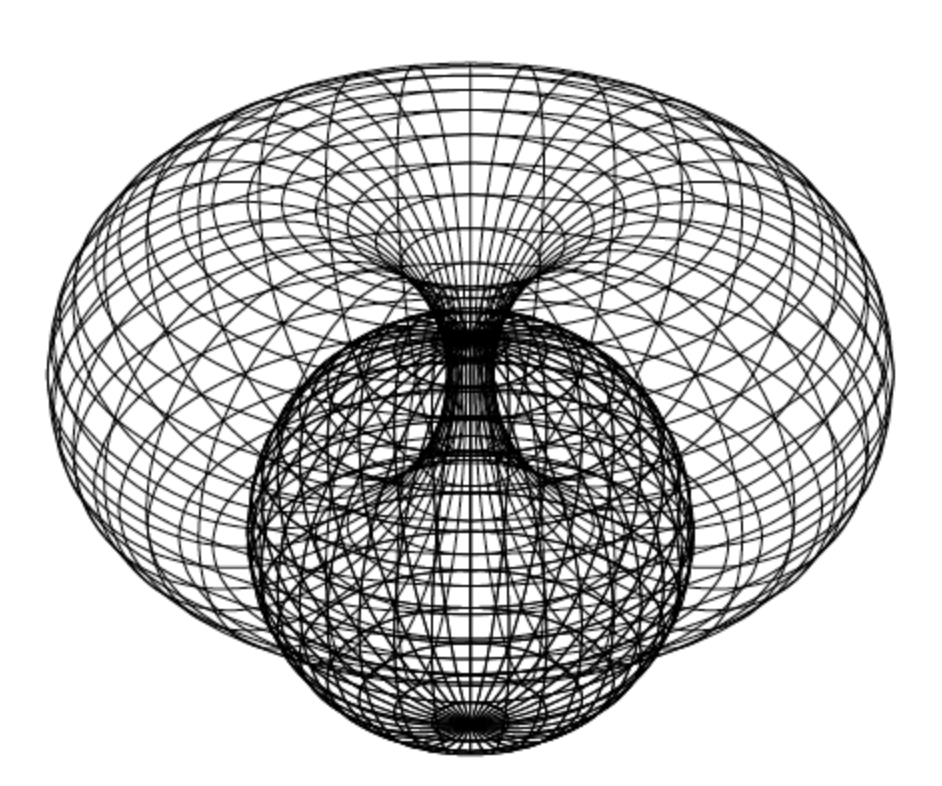
\includegraphics[scale=0.7]{./images/titlepage.png}
    \end{center}

    \vfill

    \LARGE
    Université Jean François Champollion, Albi

    \Large
    Années universitaires 2022-2025

    \vspace{0.8cm}

    \today
\end{titlepage}


\tableofcontents

\setlength{\parindent}{0pt}

% ==================================================================================================================================
% Introduction


% ==================================================================================================================================
% Inclusion Parts (Courses)


    
\part[./images/raisonnement.png]{Raisonnement et Ensembles}
\setcounter{chapter}{0}
% ==================================================================================================================================
% Raisonnement et Ensembles

% - - - - - - - - - - - - - - - - - - - - - - - - - 
%                       TITLE
% - - - - - - - - - - - - - - - - - - - - - - - - - 


% - - - - - - - - - - - - - - - - - - - - - - - - - 
%               Chapters Inclusion
% - - - - - - - - - - - - - - - - - - - - - - - - - 

\chapter{Raisonnements}
% ==================================================================================================================================
% Introduction

\minitoc

Dans ce chapitre, nous allons définir les principaux quantificateurs et connecteurs logiques utilisés en mathématiques. 
Nous aborderons différents raisonnements très utilisés pour démontrer des propriétés. 
Nous présenterons aussi la structure la plus primitive des mathématiques qui, à elle seule, peut être développée en 
toute une théorie. 

% ==================================================================================================================================
% Assertions 

\section{Assertions}

En mathématiques, syntaxiquement, on utilise ce que l'on appelle des assertions composées de quantificateurs, de noms 
et de connecteurs logiques permettant d'affirmer des choses. Une assertion (phrase) peut être vraie ou fausse. 
On note généralement une assertion $\mathcal{A}$. 

\begin{example}
    \emph{"26 est plus petit que 50"} est un assertions vraie 
\end{example}

\subsection{Quantificateurs}

Un quantificateur est un symbole mathématique permettant de donner une quantité d'un objet. 

\begin{definition}[Lettre Muette]
    Comme son num l'indique, une lettre muette est un lettre de l'alphabet (généralement $x$) muette. 
    Elle peut être remplacée par n'importe quel objet en fonction de la définition de $x$, des propriétés 
    que l'on décide qu'elle doit respecter. 
\end{definition}

\begin{example}
    Une lettre muette $a$ peut représenter la valeur $2$ ou $1$. 
\end{example}

On utilise les lettres muettes en mathématiques pour démontrer des résultats généraux. 
En manipulant des lettres muettes et en montrant des propriétés sur ces dernières, on n'a pas besoin de regarder chaque 
cas particulier. 

\begin{definition}[Quantificateur Universel]
    Le quantificateur universel $\forall$ nommé "pour tout" permet d'évoquer cette notion de généralité. 
    Dans l'assertion $\forall x \; \mathcal{A}$, on veut dire "pour toute substitution de $x$ par un objet donné, l'assertion 
    $\mathcal{A}$ est vraie". 
\end{definition}

\begin{example}
    \emph{"Pour toute voiture, celle-ci possède des roues".}
\end{example}

\begin{definition}[Quantificateur Existenciel]
    Le quantificateur existenciel $ \exists$ nommé "il existe" permet d'énoncer une propriété 
    valable pour \textbf{au moins} un éléments. 
    Ainsi, dans l'assertion $ \exists x \; \mathcal{A}$ on veut dire que "il existe au moins un élément $x$ qui vérifie la condition $ \mathcal{A}$". 
\end{definition}

\begin{example}
    \emph{L'assertion "il existe une voiture bleue est assurément vraie" tandis que l'assertion "toutes les voitures sont bleu 
    ou rouge" n'était valable qu'en URSS. }
\end{example}









\chapter{Ensembles}
% ==================================================================================================================================
% Introduction

\minitoc

Dans ce chapitre, nous allons présenter plus en détail le concept d'ensemble. 
Les ensembles sont les structures les plus primitives des mathématiques, elles permettent par exemple d'effectuer des opérations 
à l'intérieur pour ensuite définir de nouveaux objets plus complexes. 

% ==================================================================================================================================
% Définition et Égalité

\section{Généralités}

\subsection{Définition}

\begin{definition}[Ensemble]
    Un ensemble est une collection non ordonnée d'objets appelés éléments. 
\end{definition}

\textbf{L'ensemble vide}, noté $ \emptyset $, est l’unique ensemble ne contenant aucun élément. 
Un ensemble peut être vu comme un sac contenant divers éléments. 

\begin{example}
    Les entiers positifs constituent un ensemble, de même que les entiers négatifs. 
    On peut aussi parler au sens plus large de l'ensemble des jours de la semaine, ou de l'ensemble 
    des voitures bleues. 
\end{example}

\subsection{Appartenance, Inclusion, Égalité}

La théorie des ensembles est régie par une simple relation : l'appartenance. 

\begin{definition}[Appartenance]
    Soit $E$ un ensemble et $x$ un élément quelconque. 
    On dit que \emph{$x$ appartient à $E$} si $x$ est un élément de $E$. 
    On peut aussi dire que \emph{$E$ contient $x$}. On note alors 
    $x \in E$. 

    Dans le cas contraire, si "$x$ n'est pas dans $E$", on dit que 
    \emph{$x$ n'appartient pas à $E$}. 
    On note alors $x \notin E$. 
\end{definition}

Par extension, on peut définir les notions d'inclusion et d'égalité entre ensembles. 

\begin{definition}[Inclusion]
    Soient $E, F$ deux ensembles. On dit que $F$ est inclus dans $E$ ou que $E$ contient $F$ 
    si tous les éléments de $F$ appartiennent aussi à $E$. On note alors $F \subset E$. 
    Plus formellement, 
        \[ F \subset E \iff \forall x \in F, \; x \in E. \] 
\end{definition}

\begin{definition}[Égalité]
    Soient $E$ et $F$ deux ensembles. On dira qu'ils sont égaux s’ils possèdent 
    exactement les mêmes éléments. On notera alors $E = F$.
    Plus formellement, 
        \[ E = F \iff (\forall x \in E, \; x \in F) \; \text{et} \; (\forall x \in F, \; x \in E). \] 
\end{definition}

\begin{proposition}
    On peut aussi caractériser l'égalité d'ensembles en termes d'inclusions. 
    Ainsi, deux ensembles égaux peuvent aussi être vus comme deux ensembles inclus l'un dans l'autre. 
    D'où : 
        \[ E = F \iff E \subset F \text{ et } F \subset E. \]     
\end{proposition}

Pour montrer une égalité d'ensembles, on utilisera donc préférentiellement le principe de la 
double inclusion. 

% ==================================================================================================================================
% Opérations

\section{Opérations}

Définissons maintenant quelques opérations sur les ensembles. 

\begin{definition}[Opérations]
    Soit $E$ un ensemble et $A$ et $B$ deux parties de $E$. On définit les opérations suivantes : 
    \begin{itemize}
        \item On appelle \textbf{complémentaire} de $A$ dans $E$, noté $\overline{A}$, le sous-ensemble de $E$ 
        qui contient tous les éléments de $E$ qui ne sont pas dans $A$. 
            \[ \overline{A} := \{ x \in E \; | \; x \notin A \}. \] 
        \item On appelle la \textbf{différence} de $A$ par $B$ dans $E$, notée $A \setminus B$, le sous-ensemble de $E$ 
            contenant tous les éléments de $A$ qui ne sont pas dans $B$. 
            \[ A \setminus B := \{ x \in A \; | \; x \notin B \}. \] 
        \item On appelle \textbf{intersection} de $A$ et $B$, notée $A \cap B$, le sous-ensemble de $E$ 
            contenant tous les éléments à la fois dans $A$ \textbf{et} dans $B$. 
                \[ A \cap B := \{ x \in E \; | \; x \in A \text{ et } x \in B \}. \] 
        \item On appelle \textbf{union} de $A$ et $B$, notée $A \cup B$, le sous-ensemble de $E$ 
            contenant tous les éléments appartenant à $A$ \textbf{ou} à $B$. 
                \[ A \cup B := \{ x \in E \; | \; x \in A \text{ ou } x \in B \}. \] 
    \end{itemize}
\end{definition}

\begin{proposition}
    \begin{itemize}
        \item On parlera d'union disjointe de deux ensembles $A$ et $B$ lorsque leur intersection est vide. 
        \item On aura évidemment tout le temps $A \cap B \subset A$ et $A \cap B \subset B$. 
    \end{itemize}
\end{proposition}

\begin{prop}[Opérations]
    Soient $E$ un ensemble et $A, B$ et $C$ des parties de $E$. 
    On a les propriétés suivantes : 
    \begin{enumerate}
        \item Commutativité de $\cap$ et $\cup$ : 
            \[ A \cap B = B \cap A \quad \text{et} \quad A \cup B = B \cup A. \] 
        \item Associativité de $\cap$ et $\cup$ :
            \[ A \cap (B \cap C) = (A \cap B) \cap C \quad \text{et} \quad A \cup (B \cup C) = (A \cup B) \cup C. \] 
        \item Éléments neutres : 
            \[ A \cup \emptyset = A, \quad A \cap E = A, \quad A \cap \emptyset = \emptyset, \quad A \cup E = E. \] 
        \item Distributivité : 
            \[ A \cup (B \cap C) = (A \cup B) \cap (A \cup C) \quad \text{et} \quad A \cap (B \cup C) = (A \cap B) \cup (A \cap C). \] 
        \item Complémentaire involutif : $ \overline{\overline{A}} = A$. 
        \item Lois de De Morgan : 
            \[ \overline{A \cap B} = \overline{A} \cup \overline{B} \quad \text{et} \quad \overline{A \cup B} = \overline{A} \cap \overline{B}. \] 
    \end{enumerate}
\end{prop}



\begin{figure}[h!]
    \centering
    \begin{minipage}{0.45\linewidth}
        \centering
        \begin{tikzpicture}[scale=0.6]
            \begin{scope}
                \clip (-1,0) circle (1.5);
                \clip (1,0) circle (1.5);
                \fill[gray!40, opacity=0.6] (-3,-2) rectangle (3,2);
            \end{scope}
            \draw (-1,0) circle (1.5);
            \draw (1,0) circle (1.5);
            \node at (-1,-1.8) {$A$};
            \node at (1,-1.8) {$B$};
        \end{tikzpicture}
        \caption{Union $A \cup B$}
    \end{minipage}
    \hfill
    \begin{minipage}{0.45\linewidth}
        \centering
        \begin{tikzpicture}[scale=0.6]
            \begin{scope}
                \clip (-1,0) circle (1.5);
                \fill[gray!40, opacity=0.6] (1,0) circle (1.5);
            \end{scope}
            \draw (-1,0) circle (1.5);
            \draw (1,0) circle (1.5);
            \node at (-1,-1.8) {$A$};
            \node at (1,-1.8) {$B$};
        \end{tikzpicture}
        \caption{Intersection $A \cap B$}
    \end{minipage}
\end{figure}

\begin{figure}[h!]
    \centering
    \begin{minipage}{0.45\linewidth}
        \centering
        \begin{tikzpicture}[scale=0.6]
            \begin{scope}
                \clip (-1,0) circle (1.5);
                \fill[gray!40, opacity=0.6] (-3,-2) rectangle (3,2);
            \end{scope}
            \begin{scope}
                \clip (-1,0) circle (1.5);
                \fill[white] (1,0) circle (1.5);
            \end{scope}
            \draw (-1,0) circle (1.5);
            \draw (1,0) circle (1.5);
            \node at (-1,-1.8) {$A$};
            \node at (1,-1.8) {$B$};
        \end{tikzpicture}
        \caption{Différence $A \setminus B$}
    \end{minipage}\hfill
    \begin{minipage}{0.45\linewidth}
        \centering
        \begin{tikzpicture}[scale=0.6]
            % Univers E
            \fill[gray!40, opacity=0.6] (-3,-2) rectangle (3,2);
            % Ensemble A en blanc
            \fill[white] (-1,0) circle (1.5);
            \draw (-3,-2) rectangle (3,2);
            \draw (-1,0) circle (1.5);
            \node at (-1,-1.8) {$A$};
        \end{tikzpicture}
        \caption{Complémentaire $\overline{A}$}
        \end{minipage}
\end{figure}

\begin{definition}[Produit Cartésien]
    Soient $A$ et $B$ deux ensembles. On définit le produit cartésien de $A$ et $B$, noté $A \times B$, 
    comme l'ensemble composé de tous les couples possibles d'éléments de $A$ et de $B$. 
        \[ A \times B = \{(a,b) \; | \; a \in A, b \in B\} \] 
    Par définition, on dira que $(a,b) \in A \times B$ et $(c,d) \in A \times B$ sont égaux ssi 
    $a = c$ et $b = d$. 
\end{definition}

Par extension, on peut définir le produit cartésien de plusieurs ensembles $A_1, \dots A_n, n \in \N$ 
comme l'ensemble des $n$-uplets de la forme $(a_1, \dots, a_n)$ où tous les $a_i \in A_i, \forall i \in \llbracket 1, n \rrbracket$. 

% ==================================================================================================================================
% Ensemble de nombres

\section{Ensembles de nombres}

En mathématiques, nous travaillons avec différents ensembles de nombres possédant chacun différentes 
propriétés. Il est essentiel de bien les connaître ainsi que leurs relations d'inclusion. 

\subsection{Entiers Naturels}

\begin{definition}[Entiers Naturels]
    L'ensemble des entiers naturels, noté $\N$ est définit par : 
        \[ 0 \in \N \text{ et } \forall n \in \N, n + 1 \in \N \] 
    Autrement dit, $\N$ est le plus petit ensemble contenant $0$ et fermé par l'opération successeur $ : n \mapsto n+1$. 
\end{definition}

On peut aussi définir $\N$ comme l'ensemble $\N := \{1, 2, 3, \dots\}$. Nous choisissons ici d'y inclure $0$. 

\subsection{Entiers Relatifs}

\begin{definition}[Entiers Relatifs]
    On définit l'ensemble des entiers relatifs, noté $\Z$, comme : 
        \[ \Z := \{\dots, -2, -1, 0, 1, 2, \dots\} \]
    Plus formellement, $\Z$ peut être définit comme tous les nombres pouvant être formé de la soustraction 
    de deux entiers naturels. 
        \[ \Z = \{n - m \; | \; n,m \in \N\} \] 
\end{definition}

\begin{proposition}
    Cette définition permet d'en déduire les propriétés suivantes : 
    \begin{itemize}
        \item $\Z$ contient $\N$ 
        \item $\Z$ est fermé par addition et soustraction. 
    \end{itemize}
\end{proposition}

\subsection{Les Rationnels}

\begin{definition}[L'ensemble des Rationnels]
    L'ensemble des rationnels est définit comme l'ensemble des fractions d'entiers relatifs à dénominateur non nul. 
    On le note $\Q$. 
        \[ \Q := \left\{ \frac{a}{b} \; | \; a \in \Z, b \in \Z^* \right\} \] 
\end{definition}

\begin{proposition}
    $\Q$ est fermé par addition, soustraction, multiplication et division (sauf par zéro). 
\end{proposition}

\subsection{Ensemble des nombres réels}

\begin{definition}[Ensemble des nombres réels]
    L'ensemble des nombres réels, noté $\R$, est l'ensemble des limites de suites de rationnels convergentes. 
    On peut aussi le définir comme l'ensemble des nombres pouvant être représentés par une infinité décimale :
    \[
        \R := \text{complétion de } \Q \text{ pour la norme } | \cdot |.
    \]
\end{definition}

\begin{remark}
    \begin{itemize}
        \item $\R$ contient tous les rationnels (\(\Q \subset \R\)) ainsi que tous les nombres irrationnels (comme $\sqrt{2}$, $\pi$).
        \item L'ensemble $\R$ est fermé par addition, soustraction, multiplication et division (sauf par zéro).
        \item Il est ordonné et complet : toute suite croissante et bornée converge dans $\R$.
    \end{itemize}
\end{remark}

\begin{prop}[Inclusions]
    On a toujours les inclusions : 
    \[
        \N \subset \Z \subset \Q \subset \R
    \]
\end{prop}

% ==================================================================================================================================
% Cardinalité d'un ensemble

\section{Cardinalité d'un ensemble}

\begin{definition}[Ensemble fini et Cardinalité]
    Un ensemble $E$ est dit \emph{fini} s'il est vide ou s'il existe un entier naturel $n \in \N$ 
    tel qu'il existe une suite finie d'éléments de $E$, $(x_1, \dots, x_n)$, où chacun de ses éléments 
    apparaît une et une seule fois. 

    Dans ce cas, on dira que $n$ est le \emph{cardinal} de $E$. On le note $|E| = n$.
\end{definition}

\begin{proposition}
    Le cardinal $n \in \N$ d'un ensemble est unique. 
    Le cardinal de l'ensemble vide est 0. 
\end{proposition}

\begin{example}
    \[
        | \{1,2,3\} | = 3, \quad | \emptyset | = 0
    \]
\end{example}

\begin{remark}
    Pour les ensembles infinis (comme $\N$ ou $\R$), on parle de cardinal infini. 
    Deux ensembles $E$ et $F$ ont le même cardinal si une bijection (voir chap. fonctions) existe entre eux.
\end{remark}

\begin{prop}[Cardinal et Opérations]
    Soit $E$ un ensemble fini de cardinal $n \in \N$.
    \begin{itemize}
        \item Tout sous-ensemble de $E$ a un cardinal inférieur ou égal à $n$. 
        \item Si $A$ est un sous-ensemble de $E$ alors $|E/A| = |E|-|A|$. 
        \item Soient $A$ et $B$ deux sous-ensembles de $E$. On a alors : 
            \[ \boxed{| A \cup B = |A| + |B| - | A \cap B |} \] 
    \end{itemize}

\end{prop}


\chapter{Fonctions et Applications}
% ==================================================================================================================================
% Introduction

\minitoc

Les fonctions sont des objets essentiels en mathématiques. Outre leur utilité dans des domaines appliqués, elles constituent des objets mathématiques passionnants. Leur étude permet non seulement de comprendre la transformation d’éléments d’un ensemble à un autre, mais aussi de manipuler des ensembles et des relations abstraites. Dans ce cours, nous utiliserons les termes \emph{fonctions} et \emph{applications} de manière interchangeable.

% ==================================================================================================================================
% Définition et notations 

\section{Définition et notations}

Une fonction peut être vue de deux façons différentes. La première la considère comme une sorte d’entité qui permet de « transformer » une valeur ou un élément en un autre. La seconde, que nous adopterons ici, la représente comme une correspondance entre deux ensembles.

\begin{definition}[Application]
    Soient $E$ et $F$ deux ensembles. Une fonction $f$ de $E$ vers $F$ est une correspondance qui à tout élément $x$ de $E$ associe un \textbf{unique} élément de $F$, noté $f(x)$. On écrit alors : 
    \[
        f : 
        \begin{cases}
            E \longrightarrow F \\ 
            x \longmapsto f(x)
        \end{cases}
    \]
\end{definition}

\begin{figure}[h!]
    \centering
    \begin{tikzpicture}[scale=1.2, >=stealth]
        % Ensembles
        \draw (0,0) ellipse (1 and 2) node[above=2.5cm] {$E$};
        \draw (5,0) ellipse (1 and 2) node[above=2.5cm] {$F$};

        % Points dans E
        \node (e1) at (0,1.2) {$e_1$};
        \node (e2) at (0,0.4) {$e_2$};
        \node (e3) at (0,-0.4) {$e_3$};
        \node (e4) at (0,-1.2) {$e_4$};

        % Points dans F
        \node (f1) at (5,1.2) {$f_1$};
        \node (f2) at (5,0.4) {$f_2$};
        \node (f3) at (5,-0.4) {$f_3$};
        \node (f4) at (5,-1.2) {$f_4$};

        % Flèches de la fonction
        \draw[->] (e1) -- (f2);
        \draw[->] (e2) -- (f1);
        \draw[->] (e3) -- (f2);
        \draw[->] (e4) -- (f4);
    \end{tikzpicture}
    \caption{Représentation sagittale d'une fonction $f : E \to F$}
\end{figure}

\begin{remark}
    Soit $f : E \longrightarrow F$ une fonction et $a \in E$, $b \in F$. 
    \begin{itemize}
        \item L'ensemble $E$ est appelé \emph{ensemble de départ} ou \emph{domaine} de $f$.
        \item L'ensemble $F$ est appelé \emph{ensemble d'arrivée} ou \emph{codomaine} de $f$.
        \item Si $f(a) = b$, on dira que \emph{$a$ est un antécédent de $b$ par $f$} et que \emph{$b$ est l'image de $a$ par $f$}.
    \end{itemize}
\end{remark}

\textbf{Attention :} pour une fonction $f : E \longrightarrow F$ et $x \in E$, il ne faut pas confondre $f$, l’application en tant que correspondance, et $f(x)$ qui est un élément de $F$.

% ------------------------------------------------------------------
% Exemple fonction carré

\begin{example}[Fonction carré]
    Soit la fonction 
    \[
        f : \R \longrightarrow \R, \quad x \longmapsto x^2.
    \]

    \begin{minipage}{0.45\textwidth}
        \centering
        \begin{tikzpicture}
            \begin{axis}[
                axis lines = middle,
                xlabel = $x$,
                ylabel = {$f(x)=x^2$},
                xmin=-3, xmax=3,
                ymin=-0.5, ymax=9,
                samples=200,
                domain=-3:3,
                width=7cm, height=5cm,
                enlargelimits
            ]
                \addplot[blue, thick] {x^2};
            \end{axis}
        \end{tikzpicture}
        \captionof{figure}{Graphe de la fonction carré}
    \end{minipage}
    \hfill
    \begin{minipage}{0.45\textwidth}
        C'est une application : à chaque réel $x$ correspond un unique réel $f(x) = x^2$. \\
        Domaine : $\R$, Codomaine : $\R$. \\
        Image : l'ensemble des réels positifs ou nuls :
        \[
            f(\R) = \{ y \in \R \mid y \geq 0 \}.
        \]
        Quelques valeurs :
        \[
        \begin{array}{c|c|c|c|c|c}
        x & -2 & -1 & 0 & 1 & 2 \\ \hline
        f(x) & 4 & 1 & 0 & 1 & 4
        \end{array}
        \]
        On voit que $4$ est l'image de $2$ et de $-2$, et que $\sqrt{2}$ est un antécédent de $2$.
    \end{minipage}
\end{example}

% ------------------------------------------------------------------
% Image et préimage

\begin{definition}[Image et préimage]
    Soit $f : A \longrightarrow B$ une fonction.
    \begin{itemize}
        \item \textbf{L'image directe} d'un sous-ensemble $X \subset A$ par $f$ est :
        \[
            f(X) := \{ f(x) \mid x \in X \}.
        \]
        \item \textbf{La préimage} d'un sous-ensemble $Y \subset B$ par $f$ est :
        \[
            f^{-1}(Y) := \{ x \in A \mid f(x) \in Y \}.
        \]
    \end{itemize}
\end{definition}

\begin{example}
    Soit $E = \{1,2,3\}$, $F = \{a,b\}$ et $f$ définie par $f(1)=a$, $f(2)=a$, $f(3)=b$.
    \[
        f(E) = \{a,b\}, \quad f^{-1}(\{a\}) = \{1,2\}, \quad f^{-1}(\{b\}) = \{3\}.
    \]
\end{example}

% ------------------------------------------------------------------
% Composition

\begin{definition}[Composition de fonctions]
    Soient $f : E \longrightarrow F$ et $g : F \longrightarrow H$. La \emph{composition} $g \circ f : E \longrightarrow H$ est définie par :
    \[
        \forall x \in E, \quad g \circ f (x) := g(f(x)).
    \]
\end{definition}

\begin{example}
    Soient $f(x) = x^2$ et $g(x) = x+1$. Alors :
    \[
        g \circ f (x) = g(f(x)) = x^2 + 1.
    \]
\end{example}

% ------------------------------------------------------------------
% Préparation à l'injection et la surjection

\begin{remark}
    Avant d’introduire l’injectivité et la surjectivité, on peut observer que :
    \begin{itemize}
        \item Certains éléments du codomaine peuvent avoir plusieurs antécédents (ex. $4$ pour $f(x)=x^2$).
        \item Certains éléments du codomaine peuvent ne pas être atteints par la fonction (ex. $-2$ pour $f(x)=x^2$).
    \end{itemize}
    Ces observations motivent la définition des fonctions injectives et surjectives.
\end{remark}


% ==================================================================================================================================
% Injection et Surjection

\section{Injection et Surjection}

Comme nous l'avons observé avec la fonction carré, certains éléments du codomaine peuvent avoir plusieurs antécédents et certains éléments peuvent ne pas être atteints. Cela conduit naturellement aux notions d'\emph{injection}, \emph{surjection} et \emph{bijection}.

% ------------------------------------------------------------------
% Fonction injective

\subsection{Fonction Injective}

\begin{definition}[Fonction injective]
    Une fonction $f : E \longrightarrow F$ est dite \emph{injective} si des images égales impliquent des antécédents égaux. Formulée autrement :
    \[
        \forall x,y \in E, \quad f(x) = f(y) \implies x = y.
    \]
\end{definition}

\begin{remark}
    L'injectivité garantit que chaque élément de l'image provient d'un seul élément du domaine. Intuitivement, la fonction ne "fusionne" pas d'éléments distincts du domaine sur le même élément du codomaine.
\end{remark}

\begin{example}[Fonction injective]
    La fonction $f : \R_+ \longrightarrow \R$ définie par $f(x) = x^2$ est injective :
    \[
        f(2) = 4, \quad f(3) = 9, \quad f(4) = 16
    \]
    et chaque valeur de l'image correspond à un unique antécédent.
\end{example}

% ------------------------------------------------------------------
% Fonction surjective

\subsection{Fonction Surjective}

\begin{definition}[Fonction surjective]
    Une fonction $f : E \longrightarrow F$ est dite \emph{surjective} si chaque élément du codomaine est atteint par au moins un antécédent :
    \[
        \forall y \in F, \exists x \in E \text{ tel que } f(x) = y.
    \]
\end{definition}

\begin{remark}
    La surjectivité garantit que l'image couvre tout le codomaine. Intuitivement, aucun élément du codomaine n'est "laissé de côté".
\end{remark}

\begin{example}[Fonction surjective]
    La fonction $f : \R \longrightarrow \R_+$ définie par $f(x) = x^2$ est surjective, car tout réel positif possède au moins un antécédent.
\end{example}

% ------------------------------------------------------------------
% Fonction bijective

\subsection{Fonction Bijective}

\begin{definition}[Fonction bijective]
    Une fonction $f : E \longrightarrow F$ est dite \emph{bijective} si elle associe 
    à chaque élément de $F$ un unique antécédant de $E$. 
    On peut alors construire sa \emph{fonction inverse}, notée $f^{-1}$ telle que : 
        \[ f^{-1} : 
            \begin{cases}
                F \longrightarrow E \\ 
                f(x) \longmapsto x 
            \end{cases} \] 
\end{definition}

\begin{proposition}
    Pour toute fonction bijective $f : E \longrightarrow F$, on a donc : 
        \[ \forall x \in E, f^{-1}(f(x)) = x, \quad \forall y \in F, f(f^{-1}(y)) = y \] 
\end{proposition}

\begin{example}[Fonction bijective]
    La fonction $f : \R \longrightarrow \R$ définie par $f(x) = x + 1$ est bijective d'inverse. 
    \[
        f^{-1}(y) = y-1, \quad \forall y \in \R.
    \]
\end{example}

\begin{prop}[Caractérisation]
    Une fonction $f : E \longrightarrow F$ est bijective si et seulement si elle est \emph{injective} et \emph{surjective}.
\end{prop}

\begin{proposition}
    Les bijections nous permettent de faire le lien avec la théorie des ensembles. 
    En effet, deux ensembles fini $A$ et $B$ sont de même cardinal s'ils peuvent être mis en bijection. 
\end{proposition}

On peut maintenant définir la notion d'ensemble dénombrable. 

\begin{definition}[Ensemble dénombrable]
    Un ensemble $E$ est dit \emph{dénombrable} s'il peut être mis en bijection avec l'ensemble des
    entiers naturels $\N$. 
\end{definition}








\part[./images/algebre_struct.png]{Algèbre des Structures}
\setcounter{chapter}{0}
% ==================================================================================================================================
% Algèbre des Structures 

% - - - - - - - - - - - - - - - - - - - - - - - - - 
%                       TITLE
% - - - - - - - - - - - - - - - - - - - - - - - - - 


% - - - - - - - - - - - - - - - - - - - - - - - - - 
%               Chapters Inclusion
% - - - - - - - - - - - - - - - - - - - - - - - - - 

\chapter{Groupes, Sous-Groupes}
% ==================================================================================================================================
% Introduction

\minitoc  % Affiche la table des matières pour ce chapitre

Grâce au cours de raisonnement et ensemble, nous connaissons bien la notion d'ensemble et les propriétés qu'ils ont. 
Cependant cette structure reste primitive et on commence à en faire le tour. 
Essayons maintenant de doter notre ensemble de quelques propriétés supplémentaires et d'une loi entre ses éléments. 

% ==================================================================================================================================
% Groupes

\section{Groupes}

\begin{definition}[Groupe]
    Un groupe est un couple $(G,*)$ où $G$ est un ensemble et $*$ une application telle que $* : G \times G \rightarrow G$, que l'on appelle loi de composition interne.
    Une groupe satisfait les conditions suivantes :
    \begin{enumerate}
        \item \textbf{$*$ est associative} : $ \forall x, y, z \in G, \; x * (y * z) = (x * y) * z $
        \item \textbf{G est muni du neutre pour $*$} : $ \exists e \in G, \forall x \in G, \; x * e = e * x = x $ 
        \item \textbf{G est inversible} : $ \forall x \in G, \exists y \in G, \; x * y = y * x = e $
    \end{enumerate}
\end{definition}

\begin{remark}
    \begin{itemize}
        \item Le groupe $(G,*)$ est dit \textbf{abélien} ou commutatif ssi $ \forall g,h \in G, g*h = h*g $.
        \item \textbf{L'ordre} de $G$, noté $|G|$, est le cardinal de l'ensmeble si celui-ci est fini. Sinon on dit que $G$ est d'ordre infini.
    \end{itemize}
\end{remark}

\begin{definition}[Groupe Produit]
    Soient $(G_1, *)$ et $(G_2, *)$ deux groupes. On appelle groupe produit le groupe $(G_1 \times G_2, *)$ de $G_1$ et $G_2$ en posant : \[ (x_1, x_2) * (y_1, y_2) = (x_1 * y_1, x_2 * y_2) \]
\end{definition}

% ==================================================================================================================================
% Sous-groupes

\newpage
\section{Sous-groupes}

Lorsque l'on a un groupe, on peut définir d'autre groupes à l'intérieur de celui-ci appelé sous-groupe. 
En général, pour montrer qu'une structure sur un ensemble connu est un groupe on essaye d'abord de montrer que c'est un 
sous-groupe d'un groupe connu. 

\begin{definition}[Sous-groupes]
    Un sous-groupe d'un groupe $G$ est un sous-ensemble $H$ de $G$ sur lequel la multiplication de $G$ induit une structure groupe.
    Il vérifie les propriétés suivantes :
    \begin{itemize}
        \item $ e_G \in H $
        \item $ \forall x, y \in H, \; x * y \in H $
        \item $ \forall x \in H, \; x^{-1} \in H $
    \end{itemize}
\end{definition}

\begin{theorem}[Neutre et inverse dans une sous-groupe]
    Si $H$ est un sous groupe de $G$, le neutre de $H$ est le même que le neutre de $G$ et l'opposé dans $H$ est le même que l'opposé dans $G$.
\end{theorem}

\begin{proposition}[CNS Sous-groupe]
    Soit $(G,*)$ un groupe. Une partie $H$ de $G$ est un sous-groupe de $G$ ssi :
    \begin{itemize}
        \item $H \not = \emptyset $
        \item $ \forall h_1, h_2 \in H, h_1 * h_2^{-1} \in H $
    \end{itemize}
\end{proposition}


\begin{definition}[Sous-groupe distingué]
    Un sous-groupe $H$ de $(G,*)$ est dit \textbf{distingué} ssi 
        \[ \forall g \in G, \forall h \in H, \quad ghg^{-1} \in H \] 
    On le notera $ H \triangleleft G $
\end{definition}

\begin{remark}(Cas particulier des sous-groupes distingués)
    \begin{itemize}
        \item Pour tout groupe G, $\{ e \} \triangleleft G$ et $G  \triangleleft G$
        \item Une sous-groupe d'un groupe abélien est toujours distingué. 
    \end{itemize}
\end{remark}

\begin{definition}[Groupe Simple]
    Un groupe $G \not = \{ e \}$ est appelé groupe simple si les seuls groupes distingués de $G$ sont les sous-groupes triviaux $\{ e \}$ et $G$.
\end{definition}

\begin{proposition}
    L'intersection de sous-groupes distingués (ou non) de $G$ est une sous-groupe distingué (ou non) de $G$.
\end{proposition}

\newpage

% ==================================================================================================================================
% Sous-groupe engendré

\section{Sous-groupe engendré}

Dans certains espaces, on peut définir un groupe à partir d'un unique élément (ou de plusieurs) ce qui donne des 
groupes très intéressant à étudier. 

\begin{definition}[Sous-groupe engendré]
    Soit $(G,*)$ un groupe et $X$ une partie de $G$. Il existe un plus petit sous-groupe de $G$ contenant $X$ appelé sous-groupe engendré par $X$ et noté $\langle X\rangle $.

    Un groupe fini est appelé \textbf{groupe cyclique} s'il existe $g \in G$ tel que $\langle g\rangle =G$.

    Nous appelons l'ordre d'un élément $g \in G$ l'ordre du sous-groupe $\langle g\rangle $, engendré par $g$.
\end{definition}

\begin{corollary}
    Soient $(G,*)$ un groupe et $g \in G$ un élément d'ordre fini $n \in \N$. Alors $n$ ets le plus petit entier strictement positif ayant la propriété $g^n = e$ et de plus : 
        \[ \langle g\rangle  = \{ g, g^2, g^3, \dots, g^n=e \} \] 
\end{corollary}

\begin{proposition}[Sous-groupe des entiers]
    Soit $H$ un sous-groupe de $(\Z,+)$, alors il existe un unique $n \in \Z$ tel que $ H = n\Z$.
\end{proposition}


\chapter{Groupe Symétrique}
\input{subjects/Algebre-Structures/chapitres/chapitre2_Groupe_Symétrique.tex}

\chapter{Morphismes de Groupes}
% ==================================================================================================================================
% Introduction

\minitoc  % Affiche la table des matières pour ce chapitre

En mathématiques, dès que l'on découvre une nouvelle structure particulière, on essaye de définir des applications dessus 
pour essayer de voir si certaines structures se ressemblent ou pas. C'est ce que l'on va faire avec les groupes. 

% ==================================================================================================================================
% Morphisme, Image et Noyaux 

\section{Morphismes, Image et Noyaux}

\subsection{Définitions Générales et premières propriétés}

\begin{definition}[Morphisme de groupes]
    Soient $(G,\ast )$ et $(K,\bullet )$ deux groupes. 
    Un morphisme de groupes $\phi$ entre $G$ et $K$ est une application 
        \[ \phi : 
        \begin{cases}
            G \longrightarrow K \\ 
            g \longmapsto \phi(g)
        \end{cases} \] 
        telle que : 
        \[ \forall (g_1,g_2) \in G \times G, \quad \phi (g_1 \ast g_2) = \phi(g_1) \bullet \phi(g_2) \]
    \emph{"Un morphisme de groupes est une application qui respecte la structure des groupes."}
\end{definition}

\newpage 

\begin{definition}[Noyau et Image]
    Soit $\phi$ un morphime entre deux groupes $(G,*)$ et $(K,\bullet)$. 
    \begin{itemize}
        \item Le \textbf{noyau} de $\phi$ est l'ensemble des éléments de $G$ envoyés par $\phi$ sur $e_{K}$ 
            \[ \text{i.e } \ker (\phi) = \{ g \in G, \quad  \phi(g) = e_{K} \} \] 
        \item \textbf{L'image} de $\phi$ est l'ensemble des $\phi(g), g \in G$ dans $K$. 
            \[ \text{i.e }  \phi(G) = \{ h \in K, \quad \exists g \in G \text{ tq } \phi(g) = h \} \] 
    \end{itemize}
\end{definition}

\begin{definition}[Morphismes et bijection]
    \begin{itemize}
        \item Un \textbf{isomorphime} de $G$ dans $K$ est un morphisme de groupes \textbf{bijectif}. 
        \item Un \textbf{endomorphisme} de $G$ est un morphisme de $G$ dans lui-même. 
        \item Un \textbf{automorphisme} de $G$ est un morphisme bijectif de $G$ dans lui-même. 
    \end{itemize}
\end{definition}

\begin{prop}[Morphismes]
    Soit $\phi : (G,*) \longrightarrow (K,+)$ un morphisme de groupes. 
    \begin{itemize}
        \item $\phi (e_g) = e_{K} $
        \item $\phi(g^{-1}) = \phi(g)^{-1}$
        \item $\phi(g^n) = \phi(g)^n$
    \end{itemize}
\end{prop}

\subsection{Image et Noyaux}

\begin{lemma}[Image et Image réciproque d'un morphisme]
    Soit $\phi : (G,*) \longrightarrow (K,\bullet)$ un morphisme de groupes. 
    \begin{itemize}
        \item L'image d'un sous-groupe $H$ de $G$ est un sous-groupe de $G$. 
        \item Si $H \vartriangleleft G$ alors $\phi(H) \vartriangleleft \phi(G)$ \\ 
        En particulier, si $\phi$ est surjectif, alors $\phi(H) \vartriangleleft K$ 
        \item L'image réciproque d'un sous-groupe de $K$ est un sous-groupe de $G$.
        \item Si $H' \vartriangleleft G'$ alors $\phi^{-1}(H') \vartriangleleft G$ 
    \end{itemize}
    De plus, l'image de $\phi$ est un sous-groupe de $K$ et $\ker(\phi)$ est un sous-groupe distingué de G.
\end{lemma}

\begin{corollary}[Morphisme et sous-groupe engendré]
    Soit $\phi : (G,*) \longrightarrow (K,+)$ un morphisme de groupes et $X \subset G$, alors 
        \[ \boxed{ \phi(\langle  X \rangle ) =  \langle \phi(X) \rangle } \] 
    \emph{"L'image d'un générateur est le générateur de l'image."}
\end{corollary}

\begin{prop}[Stabilité]
    Les morphismes de groupes sont stables par composition et réciproque (dans le cas d'un isomorphisme).
\end{prop}

\begin{lemma}
    Un morphisme de groupes $\phi : G \longrightarrow K$ est injectif si et seulement si $\ker(\phi) = \{e_{G}\}$.
\end{lemma}

\subsection{Le cas des entiers}

\begin{proposition}
    Il existe un unique groupe cyclique d'ordre $n \in \N$  (à isomorphisme près). 
\end{proposition}

\begin{theorem}[Ordre Fini]
    Soit $G$ un groupe et $g \in G$. 
    \begin{enumerate}
        \item $g$ est d'ordre \textbf{infini} ssi $\langle g \rangle \sim (\Z,+)$, dans ce cas :
            \[ \langle g \rangle = \{\dots, g^{-3}, g^{-2}, g^{-1}, e, g, g^2, g^3, \dots \} \] 
        \item $g$ est d'ordre \textbf{fini} $n \in \N$ si et seulement si l'ensemble $\langle g \rangle = \{e, g, g^2, \dots, g^{n-1}\}$ 
        est bien défini et si $g^n = e$.
    \end{enumerate}
\end{theorem}

% ==================================================================================================================================
% Automorphisme 

\section{Automorphismes}

Pour rappel, un automorphisme d'un groupe G est un morphisme de groupe bijectif de G dans lui-même.

\begin{definition}[Centre d'une groupe]
    Le centre d'un groupe $G$ est l'ensemble $Z(G)$ des éléments de $G$ qui commutent avec tous les éléments de $G$.
\end{definition}

\begin{theorem}[Automorphismes]
    L'ensemble $(Aut(G),\circ)$ des automorphismes d'un groupe $G$ muni de la composition, est un groupe.
    \begin{itemize}
        \item C'est un sous-groupe de l'ensemble des permutations de $G$. 
        \item Si $G$ est d'ordre fini $n$, alors $Aut(G)$ est un groupe d'ordre au plus $(n-1)!$.
    \end{itemize}
\end{theorem}

\begin{definition}[Automorphisme intérieur]
    Soit $(G,\ast)$ un groupe noté multiplicativement, on définit l'automorphisme intérieur associé à $g \in G$ le morphime
    de groupes tel que :
    \[  Int_g
        \begin{cases}
            G \longrightarrow G \\
            x \longmapsto gxg^{-1}
        \end{cases}
    \]
    On définit $Int(G)$ comme l'ensemble des automorphismes intérieurs de $G$.
\end{definition}

\begin{remark}
    \begin{itemize}
        \item Tout automorphisme intérieur est un automorphisme de groupes. 
        \item Deux éléments d'un groupes dont l'un est image de l'autre par automorphisme intérieur sont dits conjugués. 
        \item On remarquera qu'un sous-groupe H de G est distingué dans G ssi H est stable par tous les automorphismes intérieurs de G. 
    \end{itemize}
\end{remark}


\chapter{Théorème de Lagrange}
% ==================================================================================================================================
% Introduction

\minitoc  % Affiche la table des matières pour ce chapitre

Joseph Louis de Lagrange était un mathématicien, astronome et mécanicien italien de la fin du XVIII° siècle. 
Né en 1736 à Turin en Sardaigne, il mourut en 1813 à Paris. Initiateur du Calcul des Variations, il étudia la mécanique de l'artillerie, 
l'astronomie, au travers des variations de l'orbite lunaire, l'analyse et se trouva très fort en arithmétique. 
On lui doit le Théorème des Quatre Carrés et le Théorème de Lagrange sur les groupes d'ordre fini. 

La théorie des groupes n'existant pas à son époque, puisqu'elle émergeat qu'au XIX°s sous l'impulsion de Cauchy, Gauss et Galois,
Lagrange n'énonça pas son théorème tel que nous allons le voir, mais il lui est quand même dû.

% ==================================================================================================================================
% Relation d'équivalence 

\section{Relation d'équivalence}

De légers rappels sur les relations et les classes d'équivalences ne sont jamais de trop... 

\begin{definition}[Relation d'équivalence]
    Une relation d'équivalence $\sim$ entre deux éléments $x$ et $y$ d'un ensemble $X$ est une relation (RST):
    \begin{itemize}
        \item \textbf{Réflexive : } $x \sim x$ 
        \item \textbf{Symétrique :} $x \sim y \Longleftrightarrow y \sim x$ 
        \item \textbf{Transitive : } $ \forall z \in X, x \sim y $ et $y \sim z \Longrightarrow x \sim z $
    \end{itemize}
\end{definition}

\begin{remark}
    Etre isomorphe est une relation d'équivalence sur les groupes. 
\end{remark}

\begin{definition}[Classes d'équivalence]
    Soit $\sim$ une relation d'équivalence sur un ensemble $X$. Une classe d'équivalence de $x \in X$, 
    souvent noté $\overline{x}$ est l'ensemble :
    \[ \overline{x} = \{y \in X, x \sim y\}\]
\end{definition}

\begin{remark}
    On remarquera que les classes d'équivalences sur un ensemble forment une partition de cet ensemble. 
\end{remark}

\begin{definition}[Projection Canonique]
    Soit $\sim$ une relation d'équivalence sur un ensemble $X$. On appelle \textbf{ensemble quotient de $X$ par $\sim$} l'ensemble :
        \[ X / \sim = \{\overline{x}, x \in X \} \]
    On définit alors la \textbf{projection canonique} comme l'application :
        \[ \pi :
            \begin{cases}
                X \longrightarrow X / \sim \\ 
                x \longmapsto \overline{x} 
            \end{cases}
        \]
    \emph{"C'est l'application, qui, à x lui associe sa classe d'équivalence pour la relation $\sim$."}
\end{definition}

\begin{remark}
    La projection canonique est surjective puisqu'une classe d'équivalence n'est jamais vide. 
\end{remark}

% ==================================================================================================================================
% Classes à gauche 

\section{Classes à gauche}

\begin{definition}[Classe à gauche]
    Soit G un groupe noté multiplicativement et H un sous-groupe de G. La relation $\sim_H$ est une relation d'équivalence sur G telle que :
        \[ \forall g_1,g_2 \in G, \quad g_1 \sim_H g_2 \Longleftrightarrow \exists h \in H, g_1 = h.g_2 \] 
    Ses classes d'équivalences sont les ensembles $gH$ notés $gH = \{ gh, h \in H \}$ de G. On les appelles \textbf{classes de $g$ à gauche} de
    G modulo H.
\end{definition}

\begin{remark}
    On peut définir de façon similaire les classes à droite de G modulo H, mais dans la pratique, nous n'utiliserons que les classes à gauche. 
\end{remark}

\begin{prop}[Classes à gauche et cardinal]
    Soit G un groupe et H un sous-groupe de G. Toutes les classes à gauche de G modulo H ont le même cardinal que H.
\end{prop}

\begin{quote}
	\footnotesize
	\begin{proof}
        Montrons que toutes les classes à gauche de G modulo H sont isomorphes à H.
		Soit $g \in G$. Considérons $\phi_g$ l'application telle que  :
            \[ \phi_g :
                \begin{cases}
                    H \longrightarrow gH \\
                    h \longmapsto gh 
                \end{cases}
            \] 
        \begin{enumerate}
            \item \textbf{Injectivité :} Soient $h_1,h_2 \in H$ tels que :
                \begin{align*}
                    & \phi(h_1) = \phi(h_2) \\
                    \Longleftrightarrow \; & g h_1 = g h_2 \\ 
                    \Longleftrightarrow \; & h_1 = h_2
                \end{align*}
            \item \textbf{Surjectivité :} Soit $x \in gH$, $ \exists h \in H$ tel que $\phi(h) = gh = x$
        \end{enumerate}
        Donc $\phi$ est bijective. D'où le résultat. 
    \end{proof}
	\normalsize
\end{quote}

\newpage 
\subsection{Ensemble Quotient et Indice}

\begin{definition}[Ensemble Quotient]
    Soit $(G,.)$ un groupe noté multiplicativement et $H \leq G$. L'ensemble quotient de $G$ par la relation d'équivalence 
    $\sim_H$, noté $G/H$ est l'ensemble $\{gH, \; g \in G\}$ des classes à gauche de G modulo H. 

    \vspace{0.5cm}

    \textbf{L'indice} de H dans G, noté $(G:H)$ est le cardinal de l'ensemble quotient $G/H$.
    Il correspond au nobre de classes d'équivalences différentes pour la relation $\sim_H$ dans G. 
\end{definition}

\begin{theorem}[Cardinal du groupe et ensemble quotient]
    Soit $(G,.)$ un groupe et $H \leq G$ alors : 
        \[ |G| = |H| \times (G:H) \]
\end{theorem}

\subsection{Théorème de Lagrange appliqué aux groupes finis}

\begin{theorem}[Théorème de Lagrange]
    Soit G un groupe fini et $H \leq G$, alors {l'ordre de H divise l'ordre de G}.
\end{theorem}

\begin{corollary}[Ordre d'un élément]
    Soit G un groupe d'ordre fini et $g \in G$ alors $ \text{ord}(g) \mid  \text{Card}(G)$. 
\end{corollary}

\begin{proposition}[Sous-groupe d'indice 2]
    Soit G un groupe et $H \leq G$, si H est d'indice 2 alors il est distingué dans G. 
\end{proposition}

\begin{quote}
	\footnotesize
	\begin{proof}
        Soit $g \in G$. Distinguons deux cas :
        \begin{itemize}
            \item si $g \in H$ alors comme H est un sous-groupe $ \forall h \in H, ghg^{-1} \in H$ 
            \item si $g \in G \backslash H$. H est d'indice 2 donc G n'a que deux classes modulo H, 
            $H = eH = He$ et puisque les classes forment une partition de G, $G \backslash H$ forme la deuxième classe 
            à gauche et à droite. 

            Donc $G \backslash H = gH = Hg$ et $ \forall h \in H, \; \exists h' \in H$ tel que $gh = h'g$. 

            C'est à dire que $ghg^{-1} = h' \in H$. 
        \end{itemize}
        Donc $H \triangleleft G$. 
    \end{proof}
	\normalsize
\end{quote}

\chapter{Actions de Groupes}
% ==================================================================================================================================
% Introduction

\minitoc  % Affiche la table des matières pour ce chapitre

Depuis le début de l'étude des groupes nous voyons ces objets simplement comme des ensembles auxquels ont 
a donné une structure via une application et quelques autres propriétés. Ces objets, en apparence très simples, 
sont pourtant très riches et peuvent être très variés. 

Une autre approche de l'étude de la théorie des groupes est de les faire agir sur un ensemble. L'un des exemples 
le plus intuitif pour comprendre cette notion est le groupe symétrique. En effet, il est définit comme l'ensemble des 
bijections sur un ensemble quelconque. Mais lorsqu'on choisit comme ensemble les entiers de 1 à $n \in \N$, on s'apperçoit
que notre groupe permute tout simplement des suites d'entier. 

% Dans ce chapitre, nous allons essayer de généraliser cette notion, en définissant tout d'abord les actions de groupes, 
% puis en démontrant quelques unes de leurs propriétés, et enfin, nous verrons comment relier ces nouvelles applications
% aux classes d'équivalences vues précédement. 

% ==================================================================================================================================
% Actions de groupes

\section{Actions de groupes, premières définitions}

\begin{definition}[Actions de groupe]
	Soit G un groupe et X un ensemble quelconque. On définit l'action à gauche de G sur X, souvent noté $ G \curvearrowright X$,
	l'application : 
		\[ \bullet : 
			\begin{cases}
				G \times X \longrightarrow X \\
				(g,x) \longmapsto g.x 
			\end{cases} \] 
	qui vérifie :
	\begin{enumerate}
		\item[i)] \textbf{Associativité Mixte :} $ \forall g,h \in G, \; \forall x \in X, \; (gh).x = g.(h.x)$ 
		\item[ii)] \textbf{Invariance par le neutre :} $ \forall x \in X, \; e_G . x = x $ 
	\end{enumerate}
	On appelle ainsi X un G-ensemble. 
\end{definition}

\begin{definition}[Point fixe et partie stable]
	Soient G un groupe et X un G-ensemble :
	\begin{itemize}
		\item $x \in X$ est un point fixe de G si, $ \forall g \in G, \; g.x = x$ 
		\item $Y \subset X$ est une partie stable de X si, $ \forall y \in Y, \forall g \in G, g(Y) \subset Y$.
	\end{itemize}
\end{definition}


% ==================================================================================================================================
% Morphisme Structurel

\section{Morphisme Structurel}

\begin{theorem}[Morphisme structurel]
	Soient G un groupe et X un G-ensemble. Il existe une bijection entre les opérations au gauche de G sur X 
	et l'ensemble des bijections de X sur lui-même ($S(X)$). 
	\[ \text{i.e} \quad 
		\begin{cases}
			G \times X \rightarrow X \\
			(g,x) \mapsto g.x
		\end{cases}
		\; \overset{\sim}{\longmapsto} \; \phi :
		\begin{cases}
			G \rightarrow S(X) \\ 
			g \mapsto \sigma_g 
		\end{cases}
	\]
	où $ \forall g \in G, \forall x \in X, \; \sigma_g(x) = g.x $
\end{theorem}


\begin{proposition}
	Soient G un groupe et $\phi$ l'action de G sur le G-ensemble X. 
	\begin{itemize}
		\item Soit $\psi$ un morphisme de groupes tq $ \psi : K \rightarrow G$, alors X est aussi un $\psi \circ \phi$-ensemble 
		(i.e on peut composer une action de groupe par la droite par un morphisme de groupe dont l'image est le groupe opérant).
		\item Soit $Y \subset X$, alors Y est aussi un G-ensemble. 
		\item Soit $H \leq G$, alors X est aussi un H-ensemble. 
	\end{itemize}
\end{proposition}

\begin{remark}
	Notons qu'une action droite d'un groupe G sur un ensemble X correspond à un anti-morphisme de groupe 
	(i.e du point de vue du morphisme structurel $ \forall g,h \in G, \phi(gh) = \phi(h)\phi(g)$).
\end{remark}

% ==================================================================================================================================
% Orbites et stabilisateurs 

\section{Orbites et Stabilisateurs}
\subsection{Définitions}

\begin{definition}[Orbite et Stabilisateur]
	Soit G un groupe et X un ensemble tels que $G \curvearrowright X$, et soit $x \in X$, on peut alors définir les deux ensembles suivants :
	\begin{itemize}
		\item \textbf{L'orbite} de x est le \underline{sous-ensemble} Orb$(x) \subseteq X$ tel que :
			\[ \boxed{ \text{Orb}_G(x) = \{g.x \; | \; g \in G\} } \] 
		\item \textbf{Le stabilisateur} de x est le \underline{sous-groupe} de G tel que :
			\[ \boxed{ \text{Stab}(x) = \{ g \in G \; | \; g.x = x \} }\] 
	\end{itemize}
	\emph{L'orbite d'un élément x de X correspond à tous les éléments de X que l'on peut atteindre sous l'action de G sur x.}
	\emph{Le stabilisateur de x de X correspond à tous les éléments de G qui laissent x invariant.}
\end{definition}

% \begin{prop}
%	Soit G un groupe et X un G-ensemble, alors le stabilisateur de $x \in X$ par G est un \textbf{sous-groupe} de G. 
% \end{prop}

\newpage 

\begin{definition}[Propriétés d'une action]
	Soit G un groupe et X un ensemble tels que $G \curvearrowright X$ on dit alors que G est :
	\begin{itemize}
		\item \textbf{Transitive} sur X s'il existe exactement une seule orbite dans X. 
		\item \textbf{Libre} sur X si tous les statbilisateurs sont triviaux (i.e réduits à l'élément neutre de G). 
	\end{itemize}
\end{definition}

\begin{prop}[Stabilité des orbites]
	Les orbites de X sont stables par G et toute union d'orbites de X est aussi stable par G. 
\end{prop}

\subsection{Orbites, stabilisateurs et relation d'équivalence}

\begin{proposition}
	Soit G un groupe et X un G-ensemble, alors :
	\begin{itemize}
		\item La relation $\sim$ définie sur X par 
			\[ x \sim y \; \text{si} \; x \in \text{Orb}(y) \] 
		est une relation d'équivalence sur X. 
		\item Les classes d'équivalences pour cette relation sont exactement les orbites de X pour l'action de G.
	\end{itemize}
\end{proposition}

\begin{prop}
	Les orbites de X par l'action de G forment une partition de X.
\end{prop}

\begin{prop}[Noyaux]
	Soient G un groupe et $\phi$ une action de groupe de G sur un ensemble X. 
	Le noyaux de $\phi$, ker$(\phi)$, est l'intersection de tous les stabilisateurs de X. 
	\[ \boxed{ \text{i.e} \quad \text{ker}(\phi) = \bigcap_{x \in X} \text{Stab}_G(x) }\] 
\end{prop}

\begin{definition}[Action fidèle]
	Soient G un groupe et X un G-ensemble pour une action $\phi$, on dit que $\phi$ est fidèle si ker$(\phi) = \{ e_G\}$. 

	\vspace{0.5cm}

	\emph{La fidélité d'une action de groupe peut être assimilé à l'injectivité.}
	
\end{definition}

% ==================================================================================================================================
% Actions Particulières

\section{Actions Particulières}
\subsection{Opération par translation}

Ici, nous allons étudier les propriétés des actions par translations. 
Jusqu'à maintenant, nous avons étudié des actions de certains groupes sur des ensembles. 
Or on peut aussi considérer un groupe comme un ensemble et donc faire agir un groupe \textbf{sur lui-même}\dots

\newpage 

\begin{definition}[Action par translation]
	Soit $(G,.)$ un groupe noté multiplicativement. On définit l'action à gauche de G sur lui-même :
		\begin{align*}
			G \times G &\longrightarrow G \\ 
			(g,h) &\longmapsto g.h = gh 
		\end{align*}
\end{definition}

\subsubsection{Théorème de Cayley}

\begin{theorem}[Cayley, 1878]
	Tout groupe fini d'ordre $n \in \N$ est isomorphe à un sous-groupe de $\mathcal{S}_n$. 
\end{theorem}

Ce théorème, bien que puissant n'est en réalité pas très utile. 
En effet pour un groupe d'ordre 6, on peut ainsi montrer qu'il est isomorhe à $\mathcal{S}_6$.
On connaît bien le groupe symétrique mais $\mathcal{S}_6$ est d'ordre $6! = 720$, au final, on ne récolte pas spécialement plus d'informations. 

\subsection{Opération par conjugaison}

Lorsque l'on a étudié le groupe symétrique, on a définit la conjugaison entre deux permuations. 
Ici, nous allons définir une action de groupe permettant de dire que deux permutations conjuguées
sont dans la même orbite..intéressant non ?

\begin{definition}[Action par conjugaison]
	Soit $(G,.)$ un groupe noté multiplicativement. On définit l'action par conjugaison de G sur lui-même :
		\begin{align*}
			G \times G &\longrightarrow G \\
			(g,h) &\longmapsto g.h = g h g^{-1}
		\end{align*}	
	On peut remarquer qu'elle est bien définie puisque $g^{-1}$ appartient bien à G. 
	Et $g h g^{-1}$ est bien dans G par stabilité. 
\end{definition}

\begin{remark}
	Permettons nous de faire quelques remarques...
	\begin{itemize}
		\item Si $G$ est abélien, alors l'action par conjugaison de G sur lui-même en triviale. 
		\item Ici, \textbf{l'orbite} d'un élément $h \in G$ est appelé \textbf{classe de conjugaison} de $h$. 
	\end{itemize}
\end{remark}

On peut ainsi définir de nouveaux objects... 

\begin{definition}[Centralisateur]
	Soit $(G,.)$ un groupe noté multiplicativement. On définit le centralisateur de $h \in G$ comme l'ensemble :
		\[ Z_G(h) = \{g \in G \; | \; ghg^{-1} = h\} \] 
	Le centralisateur d'un élément $h \in G$ peut se voir comme l'ensemble des éléments $g \in G$ qui \textbf{commutent} avec $h$.
	
	\vspace{0.3cm}

	Autrement dit, le centralisateur d'un élément est le stabilisateur du même élément pour l'action par conjugaison. 
\end{definition}

\chapter{Formule des Classes}
% ==================================================================================================================================
% Introduction

\minitoc  % Affiche la table des matières pour ce chapitre

Maintenant que nous avons vu en détail les actions de groupes, nous allons d'abord essayer de trouver des relations entre les différents ensembles qu'elles 
nous permettent de définir. 
Dans un second temps nous définirons proprement les groupes quotient du point de vue des actions de groupes, puis 
nous finirons par présenter les théorèmes d'isomorphismes. 

% ==================================================================================================================================
% Formule des classes 

\section{Formule des classes}
\subsection{Relation Orbite/Stabilisateur}

Quand on manipule des actions de groupes, on s'apperçoit vite que l'orbite d'un élément 
est étroitement lié à son stabilisateur... 

\begin{proposition}
	Soient $(G,.)$ un groupe, $X$ un ensemble et $G_x$ le stabilisateur de $x \in X$ pour l'action de G sur X. 
	Alors l'application 
		\begin{align*}
			G/G_x &\longrightarrow \text{Orb}_G(x) \\
			g G_x &\longmapsto g.x 
		\end{align*}
	Est une bijection entre l'ensemble des classes à gauche du stabilisateur de $x$ et l'orbite de x sous G. 
\end{proposition}

A partir de cette application et à l'aide du formidable outil qu'est le théorème de Lagrange, on peut en déduire le corollaire suivant... 

\newpage

\begin{corollary}[Relation Orbite/Stabilisateur]
	Soit X un  G-ensemble, $x \in X$. On utilise les mêmes notations que précédement. On a alors :
	\begin{itemize}
		\item $ | \text{Orb}_G(x) | = (G : G_x) $
		\item $ |G| = |G_x| \times \text{Orb}_G(x) $ 
	\end{itemize}
\end{corollary}

\subsection{Formules des classes}

\begin{corollary}[Formule des classes]
	Soient X G un groupe et X un G-ensemble. Alors on peut \textbf{partitionner X en orbites disjointes} sous l'action de G, d'où :
	\[ X = \bigsqcup_{i=1}^r \text{Orb}_G(x_i) \quad \text{et} \quad |X| = \sum_{i=1}^{r} |\text{Orb}_G(x_i)| = \sum_{i=1}^{r} (G : G_x) = \sum_{i=1}^{r} \frac{ |G| }{ |G_{x_i}| } \]
	où $r$ est le nombre d'orbites distinctes de X sous l'action de G. 
\end{corollary}


% ==================================================================================================================================
% Groupes Quotient 

\section{Groupe Quotient}

Nous savons déjà que le noyau d'un morphisme de groupes est un sous-groupe distingué. 
Nous cherchons ici, à partir d'un sous-groupe distingué, à construire un morphisme dont il serait le noyau. 
Pour cela, nous devons définir les groupes quotients. 

\subsection{"Quotientons !"}

Soit G un groupe et H un sous-groupe de G. On définit l'ensemble $G/H = \{gH \; | \; g \in G\}$ comme l'ensemble quotient de G par la relation d'équivalence "appartenir à la même orbite"
pour l'action par translation de H sur G. 

\begin{definition}[Projection Canonique]
	Soient G un groupe et H un sous-groupe distingué de G. La projection canonique : 
	\[\pi : 
		\begin{cases}
			G \longrightarrow G/H \\ 
			g \longmapsto gH 
		\end{cases}
	\]
	est  \textbf{morphisme de groupes} qui envoie chaque élément de G sur sa classe d'équivalence modulo la relation "appartenir à la même orbite" évoquée précédement. 
\end{definition}

\begin{theorem}[Sous-groupe distingué et projection canonique]
	Soit G un groupe. Sous H un sous-groupe de G. 
	\begin{itemize}
		\item[] H \textbf{est distingué} dans G ssi la formule $g_1H \ast g_2H = (g_1g_2)H, \; \forall g_1,g_2 \in G$ 
		définit une loi de composition interne pour l'ensemble $G/H$ telle que la projection canonique sur G est un morphisme de groupes. 
		\item[]$\iff$  $G/H$ est un groupe pour la loi $\ast$  
	\end{itemize}
\end{theorem}

\newpage 

\begin{corollary}[Ordre du quotient]
	Si H est distingué dans G, alors l'ordre du quotient de G par H est égal au quotient de l'ordre de G par l'ordre de H. 

	D'où la formule suivante :
		\[ |G/H| = \frac{|G|}{|H|} \]
\end{corollary}

\begin{corollary}[Condition nécessaire et suffisante]
	Soit G un groupe et H un sous-groupe de G. H est distigué dans G ssi H est le noyau d'un morphisme de source G. 
\end{corollary}

\begin{remark}
	Pour montrer qu'un sous-groupe est distigué, on peut donc simplement vérifier que c'est le noyau de la projection canonique $\pi$ sur G. 
\end{remark}

\subsection{Propriétés du quotient}

\begin{theorem}
	Soient G et K deux groupes et $H \triangleleft G$. Soient $\phi : G \longrightarrow K$ un morphisme de groupes 
	et $\pi$ la projection canonique sur G. Alors :
	\begin{itemize}
		\item[] $H \subset \ker(\phi)$ 
		\item[]$\iff$  $\phi (H) = \{e_K\}$ 
	\end{itemize}
	Autrement dit, on peut factoriser le morphisme $\phi$ "en passant" par $G/H$. 
	Il existe donc un morphisme de groupes $\overline{\phi} : G/H \longrightarrow K$ tel que $\phi = \overline{\phi} \circ \pi$. 
	Ainsi, $\overline{\phi}$ est unique et définit par : 
		\[\overline{\phi} : 
			\begin{cases}
				G/H \longrightarrow K \\ 
				gH \longmapsto \overline{\phi}(gH) = \phi(g)
			\end{cases}
		\]
	L'image de $\overline{\phi}$ est celle de $\phi$ et son noyau est ker($\phi$)/H.
\end{theorem}

On peut représenter cette "factorisation" par le diagramme commutatif suivant :

\begin{multicols}{2}
	\[
		\begin{tikzcd}
			G \arrow[rr, "\phi"] \arrow[dr, "\pi" swap, bend right=20] & & K \\
			& G/H \arrow[ur, "\overline{\phi}" swap, bend right=20] &
		\end{tikzcd}
	\]

	Où $H = \ker(\pi)$. 

	\vspace{0.3cm}

	Dire que le diagramme est commutatif revient à dire que $\phi = \overline{\phi} \circ \pi$

\end{multicols}

% ==================================================================================================================================
% Théorèmes d'isomorphismes 

\section{Théorèmes d'isomorphismes}

Admettons que l'on ait un morphisme $\phi : G \longrightarrow K$ entre deux groupes G et K. 
Mais $\phi$ n'est pas injectif, notons alors son noyau $H = \ker(\phi)$. Comme vu précédement, 
H est un sous-groupe de G. On va alors pouvoir construire un isomorphisme de groupe de $G/H$ dans Im$(\phi)$. 

\vspace{0.5cm}

Cela revient à assimiler tous les éléments de G comme des classes d'équivalences et ainsi, ne plus avoir le problème 
du noyau qui "envoie" plusieurs éléments sur $e_K$. 
Pour obtenir un isomorphisme il nous faut donc aussi restreindre le domaine d'arrivée aux éléments atteignables par $\phi$. 

\begin{theorem}[Premier théorème d'isomorphisme]
	Soit $\phi : G \longrightarrow K$ un morphisme de groupes. Alors il existe un isomorphisme $\overline{\psi}$ tel que :
	\[ \psi : 
		\begin{cases}
			G/\ker(\phi) \longrightarrow \text{Im}(\phi) \\ 
			g\ker(\phi) \longmapsto \phi(g)
		\end{cases}
	\]
	De plus, \textbf{si $\phi$ est surjectif}, $\psi$ est un isomorphisme entre les groupes $G/\ker(\phi)$ et $K$.
	(si $\phi$ est surjectif, on peut étendre l'image de $\psi$ à l'image de $\phi$, donc à K tout entier)
\end{theorem}

\begin{remark}
	Soit G un groupe monogène engendré par $g \in G$. 
	D'après la propriété universelle de $\Z$, il existe un morphisme $\phi : \Z \to \Longrightarrow \langle g \rangle= G$ tel que $\ker(\phi) = n\Z$. 
	
	D'après le théorème 2.2, on peut quotienter l'espace de départ par le noyau du morphisme et ainsi obtenir le morphisme suivant :
		\[ \overline{\phi} :
			\begin{cases}
				\Z/n\Z \longrightarrow \langle g \rangle \\ 
				\overline{k} \longmapsto g^k \in G 
			\end{cases}
		\] 
	Enfin, d'après le premier théorème d'isomorphisme, puisque $\phi$ est surjectif, $\overline{\phi}$ est isomorphisme. 
	D'où : $$ \langle g \rangle \simeq \Z/n\Z $$  
\end{remark}

\begin{theorem}[Troisième théorème d'isomorphisme]
	Soient $K \subset H \subset G$ trois groupes. Tels que $H \triangleleft G$ et $ K \triangleleft G$. On a alors :
		\[ (G/K)/(H/K) \simeq G/H \] 
	\emph{Autrement dit, le quotient de deux groupes quotientés par le même sous-groupe normal est isomorphe au quotient des autres groupes.}
\end{theorem}

Ce théorème mérite quelques petites explications. Notons $\sigma, \pi, \mu$ les projections canoniques associés aux groupes quotient $G/H, G/K$ et $(G/K)/(H/K)$. 

On a donc $K \subseteq H \Longrightarrow \sigma(H) = H/K$, un sous groupe de $G/K$. 
Or, d'après le théorème 2.2, il existe un unique morphisme $\overline{\sigma} : G/H \longrightarrow (G/K)/(H/K)$ tel que $\overline{\sigma} \circ \pi = \mu \circ \sigma$. 

\vspace{0.3cm}

On a donc le diagramme commutatif suivant : 

	\[
	\begin{tikzcd}[scale=1.5, row sep=3em, column sep=4em]
		G \arrow[r, "\sigma"] \arrow[d, "\pi" swap] & G/K \arrow[d, "\mu"] \\
		G/H \arrow[r, "\exists ! \overline{\sigma}" swap, dashed] & (G/K)/(H/K)
	\end{tikzcd}
	\]

$\mu$ et $\sigma$ sont surjectifs donc $\mu \circ \sigma$ est surjectif donc $\overline{\sigma}$ est surjectif. 
De plus, $\ker(\mu \circ \sigma) = H$ donc $\overline{\sigma}$ est injectif. On en conclut que $\overline{\sigma}$ est 

\begin{example}
	Quelques exemples pour mieux apprécier le théorème précédent :
	\begin{itemize}
		\item A-t-on $(\Z/10\Z)/(2\Z/10\Z) \simeq \Z/2\Z$ ? 
		\item A-t-on $(\mathcal{S}_4/\mathcal{A}_4) \simeq (\mathcal{S}_4/\mathcal{V}_4)(\mathcal{A}_4/\mathcal{V}_4)$ ?
	\end{itemize}
\end{example}

\chapter{Anneaux}
% ==================================================================================================================================
% Introduction

\minitoc  % Affiche la table des matières pour ce chapitre

Résumons, on a pris un ensemble que l'on a muni d'une opération. On a trouvé pleins de propriétés à cette nouvelle structure.
Serait-il intéressant de munir notre groupe d'une autre opération? 

% ==================================================================================================================================
% Anneaux, Définitions et Exemples

\section{Anneaux, Définitions et Exemples}

\begin{definition}[Anneaux]
    Un anneau est un ensemble $A$ muni de deux lois de composition interne généralement notées $+$ et $\times$
    tels que:
    \begin{itemize}
        \item $(A,+)$ est un groupe abélien de neutre $0_A$. 
        \item $\times$ est associative. 
        \item $\times$ est distributive à gauche et à droite par rapport à $+$. 
    \end{itemize}    
    On notera alors notre anneau $(A,+,\times)$. 
\end{definition}

\begin{definition}[Anneau Unitaire]
    Soit $(A,+,\times)$ un anneau. On dit que $A$ est unitaire si il possède un neutre $1_A$ pour la $\times$. 
    Autrement dit, si $ \exists 1_A \in A$ tel que:
        \[ \forall a \in A, \quad 1_A \times a = a \times 1_A = a \] 
\end{definition}

\begin{definition}[Anneau Commutatif]
    Soit $(A,+,\times)$ un anneau. On dit que A est commutatif si la loi $\times$ est commutative. 
    Autrement dit si: 
        \[ \forall a,b \in A, \quad a \times b = b \times a \] 
\end{definition}

\begin{example}
    Voyons quelques exemples d'anneaux :
    \begin{enumerate}
        \item $(GL_n(\R),+,\times)$ est un anneau unitaire non commutatif. 
        \item $(\Q,+,\times)$ est un anneau unitaire commutatif. 
        \item $(2\Z,+,\times)$ est un anneau commutatif non unitaire. 
    \end{enumerate}
\end{example}

\subsection{Sous-anneau}

De même que pour les groupes, on peut définir la notion de sous-anneau. Très pratique pour montrer qu'un ensemble est un 
anneau. 

\begin{definition}[Sous-anneau]
    Soient $(A,+,\times)$ un anneau et $B \subseteq A$. On dit que $B$ est un sous-anneau de $A$ si 
    \begin{itemize}
        \item $(B,+)$ est un sous-groupe de $(A,+)$ 
        \item $(B,+)$ est stable pour la loi $\times$ de $A$. 
    \end{itemize}
\end{definition}

Tout comme pour les groupes, on peut restreindre ces conditions : 

\begin{proposition}
    Soient $(A,+,\times)$ un anneau et $B \subseteq A$. B est un sous-anneau de A ssi 
    \begin{itemize}
        \item $0_A \in B$ 
        \item $ \forall x,y \in B, x+y \in B, \; -x \in B \text{ et } x \times y \in B$ 
    \end{itemize}
\end{proposition}

\begin{remark}
    Un sous-anneau d'un anneau commutatif est commutatif mais un sous-anneau d'un anneau unitaire n'est as forcément unitaire. 
\end{remark}

\begin{example}
    $(2\Z,+,\times)$ est un sous-anneau de $(Z,+,\times)$. Puisque $\Z$ est commutatif, $2\Z$ l'est aussi, 
    en revanche, puisque $1 \in \Z$ n'est pas pair, $2\Z$ n'est pas unitaire. 
\end{example}

% ==================================================================================================================================
% Calculs dans un anneau

\section{Calculs dans un Anneau}

Maintenant que nous avons muni notre groupe d'une nouvelle loi, il va falloir énoncer quelques règles de calculs. 
Puisque dans un anneau, il n'y a pas forcément d'inverse pour la loi $\times$, on ne pourra pas faire toutes les simplifications 
que l'on souhaite. 

\begin{prop}[Règles de Calculs dans un Anneau]
    Soient $a,b \in (A,+,\times)$ et $n,m \in \N$. On a les règles suivantes :
    \begin{enumerate}[label=\roman*)]
        \item $0_A \times a  = a \times 0_A = 0_A $
        \item $(na)b = a(nb) = n(ab) = nab $
        \item $(na)(mb) = (nm)(ab)$
    \end{enumerate}
    Supposons maintenant A unitaire : 
    \begin{enumerate}[label=\roman*)]
        \item $na = (n1_A)a = a(n1_A)$ 
        \item $(-1_A)^{2n} = 1_A $ et $(-1_A)^{2n+1} = -1_A $
    \end{enumerate}
\end{prop}

\begin{footnotesize}
    \begin{proof} 
        Soient $(A,+,\times)$ un anneau, $a,b \in A$ et $n,m \in \N$. 
        \begin{enumerate}[label=\roman*)]
            \item ${0_A \times a = a \times 0_A = 0_A}$ 
                \[
                    \begin{cases}
                        (b + (-b)) \times a = ba + (-ba) = 0_A \\ 
                        a \times (b + (-b)) = ab + (-ab) = 0_A
                    \end{cases}
                \]
            \item ${(na)b = a(nb) = n(ab) = nab}$
                    \begin{align*}
                        (na)b &= (a + \dots + a) b \\ 
                                &= ab +\dots + ab \\ 
                                &= n(ab)
                    \end{align*}
                    De plus, $ab + \dots + ab = n(ab)$. Par associativité on a : $(na)b = nab$  
            \item ${(na)(mb) = (nm)(ab)}$
                    \begin{align*}
                        (na)(nb) &= \underset{n\text{ fois}}{(a + \dots + a)} \underset{m\text{ fois}}{(b + \dots + b)} \\ 
                                    &= \underset{m\text{ fois}}{(ab + \dots + ab)} + \dots + \underset{m\text{ fois}}{(ab + \dots + ab)} \\ 
                                    &= n \underset{m \text{ fois}}{(ab + \dots + ab)} \\ 
                                    &= (nm)(ab)
                    \end{align*}
            \item $na = (n1_A)a = a(n1_A)$ : Supposons que $1_A \in A$. 
                    \[
                        \begin{cases}
                            (n1_A)a = \underset{n\text{ fois}}{(1_A + \dots + 1_A)} a = a + \dots + a = na \\ 
                            a(n1_A) = a \underset{n\text{ fois}}{(1_A + \dots + 1_A)} = a + \dots + a = na
                        \end{cases}
                    \]
        \end{enumerate}
    \end{proof}
\end{footnotesize}

\begin{remark}
    Soit $(A,+,\times)$ un anneau. Si A est unitaire et que $1_A = 0_A$ alors $A = \{0_A\}$. 
\end{remark}

\begin{quote}
    \begin{footnotesize}
        \begin{proof}
            Soit A un anneau unitaire tel que $0_A = 1_A$. Soit $x \in A$. Alors : 
                \[ 1_A x = 0_A x = x = 0_A \] 
            Donc $x = 0_A$ d'où $A = \{0_A\}$. 
        \end{proof}
    \end{footnotesize}
\end{quote}

\begin{proposition}[Binôme de Newton]
    Soient $(A,+,\times)$ un anneau et $a,b \in A$ tels que $a \times b = b \times a$ on a alors :
        \[ \forall n \in \N^*, \quad (a+b)^n  = \sum_{k=0}^{n} \binom{k}{n} a^k b^{n-k} = \sum_{k=0}^{n} \binom{k}{n} b^{n-k} a^k \] 
\end{proposition}

% ==================================================================================================================================
% Inverses dans un anneau

\section{Inverses dans un Anneau}

Comme nous l'avons déjà vu, un anneau ne contient pas forcément d'inverses pour la loi $\times$. 
Cela peut être le cas dans certaines situations. 
Soit $(A,+,\times)$ un anneau unitaire non nul. 

\begin{definition}[Elements Inversibles]
    Un élément $x \in A$ est dit inversible dans $A$ s'il existe $y \in A$ tel que $xy = yx = 1_A$. 
    Dans ce cas, son inverse est unique et noté $x^{-1}$. 
    On notera $\mathcal{U}(A)$ l'ensemble des éléments inversibles de $A$. Plus formellement : 
        \[ \boxed{ \mathcal{U}(A) = \{x \in A \; | \; \exists y \in A, xy = yx = 1_A \} } \] 
\end{definition}

\begin{remark}
    $\mathcal{U}(A)$ est non vide puiqu'il contient $1_A$ d'inverse lui-même. 
\end{remark}

\begin{theorem}[Structure des inverssibles]
    Soit $(A,+,\times)$ une anneau unitaire non vide, l'ensemble $\mathcal{U}(A)$ est un groupe pour la loi $\times$ 
    de A de neutre $1_A$. 
\end{theorem}

\begin{example}
    Dans l'anneau $A = (\mathcal{M}_n(\R),+,\times)$ on a $\mathcal{U}(A) = GL_n(\R)$. 
\end{example}

% ==================================================================================================================================
% Diviseurs de zéro

\section{Anneau Intègre et Diviseurs de zéro}

\begin{definition}[Diviseur de zéro]
    Soit $(A,+,\times)$ un anneau. On dit qu $x \in A$ est un diviseur de $0_A$ si :
    \begin{itemize}
        \item $x \not = 0_A$ 
        \item $ \exists y \in A/\{0_A\},$ tel que $xy = 0_A$ ou $yx = 0_A$
    \end{itemize}
    On appelle \textbf{anneau intègre} tout anneau unitaire commutatif qui n'admet pas de diviseurs de zéro. 
    Plus formellement, un anneau $(A,+,\times)$ est intègre si : 
        \[ \forall x,y \in A, \quad xy = 0_A \Longrightarrow x = 0 \text{ ou } y = 0 \] 
\end{definition}

\begin{example}
    $(\Z,+,\times)$ est intègre. En revanche $(\mathcal{M}_2(\R),+,\times)$ n'est pas intègre (utiliser les matrices nilpotentes). 
\end{example}

\begin{proposition}
    Tout sous-anneau unitaire et non nul d'un anneau intègre est intègre. 
\end{proposition}

\begin{proposition}
    Soit $(A,+,\times)$ un anneau unitaire. Si $x \in \mathcal{U}(A)$ alors $x$ n'est pas un diviseur de zéro. 
\end{proposition}

\begin{quote}
    \begin{footnotesize}
        \begin{proof}
            Soit A un anneau unitaire non trivial. Raisonnons par l'absurde. 
            Soit $x \in \mathcal{U}(A)$ un diviseur de zéro. Alors $ \exists y \in A$ non nul tel que :
                \[ xy = 0_A \Longrightarrow x^{-1}xz = z = 0 \] 
            Par hypothèse $z \not = 0_A$ donc $x$ n'est pas un diviseur de zéro. 
        \end{proof}
    \end{footnotesize}
\end{quote}

L'intégrité d'un anneau nous permet de démontrer une nouvelle règle de simplification :

\begin{prop}[Simplification dans un anneau intègre]
    Soit $A$ un anneau intègre alors $ \forall a \in A/\{0_A\}, \forall c,d \in A$, on a :
        \[ ab = ac \Longrightarrow b = c \]  
\end{prop}

\begin{quote}
    \begin{footnotesize}
        \begin{proof}
            Soient $A$ un anneau intègre, $a \in A^*$ et $b,c \in A$. Tels que $ab = ac$. Alors :
                \[ ab = ac \iff ab -ac = 0_A \iff a (b-c) = 0_A \iff a = 0 \text{ ou } b-c = 0_A \] 
                {Par hypothèse } $ a \not = 0_A$ { donc } $b-c = 0_A$ 

                {D'où : }$ b = c $
        \end{proof}
    \end{footnotesize}
\end{quote}

% ==================================================================================================================================
% Idéaux

\section{Idéaux}

Faisons la blague tout de suite, c'est pas idéal comme cours. 

\vspace{0.3cm}

Soit $(A,+,\times)$ un anneau unitaire. 

\subsection{Définitions et premiers théorèmes}

\newpage

\begin{definition}[Idéal]
    Une partie $I \subseteq A$ est un idéal à gauche de A si 
    \begin{enumerate}[label=\roman*)]
        \item $(I,+)$ est un groupe abélien 
        \item $I$ est absorbant à gauche dans $A$ 
            \[ \text{i.e} \quad \forall a \in A, \forall x \in I, \quad a.x \in I \] 
    \end{enumerate}
    Si un idéal est absorbant à gauche et à droite, on parle d'idéal bilatère. 
    Dans un anneau commutatif, tous les idéaux sont bilatères. 
\end{definition}

\begin{remark}
    Les ensembles $ \{ 0_A \}$ et $A$ sont des idéaux triviaux de $A$.  
\end{remark}

\begin{proposition}
    Une partie $I \subseteq A$ est un idéal de $A$ ssi 
    \begin{enumerate}[label=\roman*)]
        \item $0_A \in I$ 
        \item $ \forall x,y \in I, \quad x + y \in I$ 
        \item $\forall a \in A, \forall x \in I, \quad a.x \in I $ 
    \end{enumerate}
\end{proposition}

\begin{theorem}[Idéaux de $\Z$]
    Les idéaux de $\Z$ sont exactement les $n\Z$ avec $ n \in \N$. 
\end{theorem}

\begin{quote}
\begin{footnotesize}
    \begin{proof}
        Soit $n \in \N$. On a déjà montré que les $(n\Z,+)$ sont des sous-groupes de $\Z$. 
        Il suffit de montrer que ce $n\Z$ est bien un idéal de $\Z$. 

        Soit $k \in \Z$ alors $ \forall i \in n\Z$ on a : 
            \[ k \times i \times n\Z \in n\Z \]
        Donc c'est bien un idéal. 
    \end{proof}
\end{footnotesize}
\end{quote}

\begin{theorem}[C.N.S d'égalité anneau/idéal]
    Soit $I \subseteq A$ un idéal de $A$. On a alors :
        \[ I = A \iff I \cap \mathcal{U}(A) \not = \emptyset \] 
\end{theorem}

\begin{quote}
\begin{footnotesize}
    \begin{proof}
        Soit $(A,+,\times)$ un anneau unitaire et $I$ un idéal de $A$. 
        \begin{itemize}
            \item[$\boxed{\Rightarrow}$] $1_A \in A = I$ or $1_A \times 1_A = 1_A$ donc $(1_A)^{-1} = 1_A$. Donc $ I \cap \mathcal{U}(A) \not = \emptyset $
            \item[$\boxed{\Rightarrow}$] Soit $a \in I \cap \mathcal{U}(A)$ alors $ \exists a^{-1} \in A$ tel que $a^{-1}a = 1_A$. 
            Par absorption, $a^{-1}a = 1_A \in I$. Or $ \forall a \in A, a \times 1_A = a \in A$. Donc $I = A$. 
        \end{itemize}
    \end{proof}
\end{footnotesize}
\end{quote}

\subsection{Caractéristiques des Idéaux}

\begin{proposition}
    L'intersection finie d'idéaux est d'un anneau $A$ est un idéal de $A$. 
\end{proposition}

A partir de cette proposition, pour toute partie $X \subseteq A$ on sait que l'intersection de tous les idéaux de $A$ contenant 
$X$ est un idéal de $A$. 

\begin{definition}[Idéal engendré par une partie]
    Soit $(A,+,\times)$ un anneau. L'idéal engendré par X est l'intersection de tous les idéaux contenant $X$. On le note $(X)$. 
    On pourra noter $(X)_A$ pour bien identifier de quel anneaux $(X)$ est un idéal. 
\end{definition}

\begin{remark}
    Soit $X \subseteq A$ alors $(X)$ est le plus petit idéal de $A$ contenant $X$. Plus formellement, pout tout idéal $J$ de $A$ contenant $X$ 
    alors $(X) \subseteq J$. 

    \vspace{0.3cm}

    Soit $X = \{ x_1, \dots, x_p \} \subseteq A$ avec $p \in \N$. L'idéal $(X)$ est noté $x_1, \dots, x_p$. 
    On dit que $ \forall i \in \llbracket 1, p \rrbracket$, les $x_i$ sont des générateurs de $X$. 
\end{remark}

\subsection{Idéal Principal}

\begin{definition}[Idéal Principal]
    Soit $A$ un anneau et $I \subseteq A$ un idéal de $A$. On dit que $I$ est principal s'il est engendré par un set élément. 
    Autrement dit s'il existe $x \in A$ tel que $X = (x)$. 

    On dit que $A$ est principal s'il est intègre et que tous ses idéaux sont principaux. 
\end{definition}

\begin{proposition}
    Soit $A$ un anneau commutatif, unitaire et $x \in A$ alors l'idéal de $A$ engendré par $(x)$ est de la forme : 
        \[ (x) := \{ ax \; | \; a \in A \}  \] 
\end{proposition}

\begin{quote}
\begin{footnotesize}
    \begin{proof}
        Montrons que $ (x) := \{ ax \; | \; a \in A \} $ par double inclusion. 
        \begin{itemize}
            \item[$\boxed{\subseteq}$] L'ensemble $\{ ax \; | \; a \in A \} $ est un idéal de $A$ et contient $(x)$ on a donc 
            $(x) \subseteq \{ ax \; | \; a \in A \}$ par minimalité. 
            \item[$\boxed{\supseteq}$] Soit $ax \in \{ ax \; | \; a \in A \} $ alors $ax \in (x)$ par absorption et 
            car $(x)$ est un idéal qui contient $x$. 
        \end{itemize}
    \end{proof}
\end{footnotesize}
\end{quote}

\begin{theorem}[Anneau Principal et $\Z$]
    $\Z$ est un anneau principal. 
\end{theorem}

La preuve s'appuit sur le fait que $n\Z = (n)$. 

\begin{definition}[Somme d'idéaux]
    La somme d'idéaux est un idéal. Autrement dit, pour tout $I,J \subseteq A$ des idéaux de $A$, alors l'ensemble 
        \[ I + J = \{ x + y \; | \; x \in I, y \in J \} \subseteq A \]
    Est un idéal de $A$.  
\end{definition}

% ==================================================================================================================================
% Morphismes d'Anneaux

\section{Morphismes d'Anneaux} 

\begin{definition}[Morphisme d'Anneaux]
		Soient $A$ et $B$ deux anneaux unitaires. Une application $f : A \longrightarrow B$ 
		est un morphisme d'anneaux si 
		\begin{itemize} 
				\item $f$ est un morphisme du groupe $(A, +)$ dans $(B, +)$. 
				\item $\forall x, y \in A, \quad f(x \times y) = f(x) \times f(y)$ 
				\item $f(1_A) = 1_B$ 
		\end{itemize} 
		Si $f$ est, de plus bijective, on dira que c'est un \textbf{isomorphisme d'anneaux}. 
\end{definition} 

\begin{proposition} 
		Une fois que l'on a un mosphisme d'anneaux $f : (A, +, \times) \longrightarrow (B, +, \times)$,
		alors $f$ induit un morphisme de groupes entre $ (\mathcal{U}(A), \times)$ et $ (\mathcal{U}(B), \times) $. 
		Remarquons bien que nous ne parlons pas du morphisme de groupe de la définition de morphisme d'anneaux. 
\end{proposition} 

\begin{definition}[Image et Noyau]
		Soit $f : (A, +, \times) \longrightarrow (B, +, \times)$ un mosphisme d'anneaux. 
		On appelle image et noyau, l'image et le noyau du morphisme de groupes $f :  (\mathcal{U}(A), \times) \longrightarrow (\mathcal{U}(B), \times)$. 
\end{definition} 

\begin{remark} 
		On peut donc conclure de cette dernière définition que $f$ est injective ssi $ \ker f = \{0_A\}$.
\end{remark} 

\begin{prop}[Structure de l'image et du noyau]
		Soit $f : (A,+,\times) \longrightarrow (B,+,\times)$ un morphisme d'anneaux. Alors $ \ker f$ est un idéal de $A$ et 
		$Im (f)$ est un sous-anneau de $B$. 
\end{prop} 

\begin{quote} 
	\begin{footnotesize} 
		\begin{proof}

			
		\end{proof}
	\end{footnotesize} 
\end{quote} 

\begin{proposition}
		La composée de deux morphismes d'anneaux est un morphisme d'anneaux. La réciproque d'un morphisme d'anneaux bijectif 
		est aussi un morphisme d'anneaux. 
\end{proposition} 

% ==================================================================================================================================
% Anneau Quotient 

\section{Anneau Quotient}

\begin{theorem}[Quotient d'un anneau par un idéal]
    Soit $A$ un anneau unitaire non trivial et $I$ un idéal bilatère de $A$ distinct de $A$. 
    Soit $A/I$ l'ensemble des classes à gauche du groupe $(A,+)$ modulo le sous-groupe $I$. 
    On a les propriétés suivantes: 
    \begin{enumerate}[label=\roman*)]
        \item Il existe une loi de compisition interne sur $A/I$, notée $\times$ telle que :
            \[ \forall a,b \in A, \; \overline{a \times b} = \overline{a} \times \overline{b} \] 
        \item Si $+$ désigne l'addition quotient du groupe quotient $A/I$ alors $(A/I, +, \times)$ 
        est un anneau unitaire non trivial. On l'appelle anneau-quotient de $A$ par $I$. 
    \end{enumerate}
\end{theorem}

\begin{proposition}
    L'anneau quotient d'un anneau commutatif est commutatif (pour la loi $\times$). 
\end{proposition}

\begin{proposition}[Projection Canonique]
    Soit $(A/I, +, \times)$ un anneau quotient, alors l'application: 
        \[ \pi : 
            \begin{cases}
                A \longrightarrow A/I \\ 
                a \longmapsto \overline{a}
            \end{cases} \] 
    est un morphisme d'anneaux surjectif de noyau $I$. 
\end{proposition}

\begin{theorem}[Isomorphisme]
    Soit $\phi : A \longrightarrow B$ un morphisme d'anneaux. On a alors: 
        \[ \boxed{A/\ker \phi \simeq Im(\phi)} \] 
\end{theorem}

% ==================================================================================================================================
% Anneau Z/nZ 

\section{L'anneau $\Z/n\Z$}

\begin{definition}[Anneau $\Z/n\Z$]
    Soit $n \in \N, n \geqslant 2$. L'anneau des entiers modulo $n$ est l'anneau quotient de $\Z$ par on idéal $n\Z$, noté $\Z/n\Z$. 
\end{definition}

\begin{theorem}[Inversibles dans $\Z/n\Z$]
    Soit l'anneau quotient $(\Z/n\Z, +,\times)$. Les élements inversibles de cet anneau sont exactement les classes 
    dont les représentant sont premiers avec $n$. Autrement dit: 
        \[ \mathcal{U}(\Z/n\Z) = \{\overline{x} \; | \; x \in \llbracket 1, n \rrbracket \; \text{et} \; pgcd(1,n) = 1\} \] 
\end{theorem}

\begin{theorem}[Fondamental]
    Soit $n \geqslant 2$. On a: 
        \[ \boxed{n \text{ premier } \; \iff \Z/n\Z \; \text{ est un corps } \; \iff \Z/n\Z \; \text{ est intègre }} \] 
\end{theorem}

Ainsi, lorsque $n \geqslant 2$ est premier, on note $\Z/n\Z$, $\F_p$. 

\begin{proposition}
    Les diviseurs de zéro dans l'anneau $\Z/n\Z$ sont exactement les classes dont les représentants divisent $n$ 
    et qui sont strictement compris entre $1$ et $n$. 
    Autrement dit, 
        \[ \overline{d} \in \Z/n\Z \text{ est un diviseur de zéro } \iff 1 < d < n \text{ et } d|n \] 
\end{proposition}

\begin{theorem}[Chinois]
    Soient $n,m \in \N$ supérieurs à $2$. Alors: 
        \[ pgcd(n,m) = 1 \; \iff \; \Z/nm\Z \simeq (\Z/n\Z) \times (\Z/m\Z) \] 
\end{theorem}

\begin{theorem}[Petit théorème de Fermat]
    Soit $p \in \N$ premier. Pour tout $x \in \Z$, on a $x^p \equiv x \mod p$. 
\end{theorem}



\chapter{Corps}
% ==================================================================================================================================
% Introduction

\minitoc  % Affiche la table des matières pour ce chapitre

Résumons, nous avons un groupe avec une loi supplémentaire qui peut être commutative et posséder un neutre. 
Grâce à cela, nous avons pu définir les idéeaux, un nouveau type de morphisme, etc... 

Seulement, on souhaiterai pouvoir définir des structures plus complexes comme avec les groupes tels que les anneaux 
quotient, avoir une notion de divisibilité, bref, de l'arithmétique. 

Pour cela, nous avons besoin d'étendre la notion d'anneaux aux corps...

% ==================================================================================================================================
% Corps 

\section{Corps, définition et propriétés}

\begin{definition}[Corps]
    On appelle $(K, +, \times)$ un corps si $(K,+,\times)$ est un anneau et $(K^*, \times)$ un groupe. 
    Si la loi $\times$ est commutative, on parlera alors de corps commutatif. 
\end{definition}

On peut bien évidement trouver une condition nécessaire et suffisante pour qu'un anneau soit un corps...

\begin{proposition}
    Soit $(K, +, \times)$ un anneau unitaire. $K$ est un corps si tout élément non nul est inversible pour $\times$. 
    Plus formellement ssi : 
        \[ \forall x \in K^*, \; \exists y \in K, \; xy = yx = 1_K \quad \text{ssi} \; \mathcal{U}(K) = K^*\] 
\end{proposition}

\begin{proposition}
    Un corps commutatif est aussi un anneau intègre. 
\end{proposition}

Tout comme pour les groupes et les anneaux, on peut définir un sous-corps d'un corps. 

\newpage 

\begin{definition}[Sous-corps]
    Soit $K$ un corps. Un partie $L \subseteq K$ est un sous-corps de $K$ si :
    \begin{enumerate}[label=\roman*)]
        \item $L$ est un sous-anneau de $K$
        \item $1_K \in L$ 
        \item $ \forall x \in L, x^{-1} \in L$
    \end{enumerate}
\end{definition}

En pratique pour montrer qu'un anneau est un corps, on préfèrera montrer que c'est un sous-corps quand c'est possible. 

\begin{example}
    $(\C,+,\times)$ est un corps. $(\Q,+,\times)$ et $(\R,+,\times)$ en sont des sous-corps. 
\end{example}

% ==================================================================================================================================
% Anneau Quotient

\section{Anneau Quotient}

Dans cette section, on considère un anneau A unitaire, non trivial. 
On va quotienter A par un de ses idéaux I bilatère différent de A. 
On a donc le théorème suivant : 

\begin{theorem}[Structure de l'anneau quotient]
    Soit A un anneau unitaire, non trivial et I un idéal bilatère de A différent de A. 
    L'ensemble $A/I$ est définit comme l'ensemble des classes du groupe $(A,+)$ modulo le 
    sous-groupe $I$ de $A$. On définit des opérations dessus : 
    \begin{itemize}
        \item \textbf{Loi multiplicative : } $ \forall a, b \in A, \overline{a} \times \overline{b} = \overline{a \times b}$. 
        \item \textbf{Loi additive : } $ \forall a,b \in A, \overline{a} + \overline{b} \in A/I$. 
    \end{itemize}
    Alors le groupe $(A,+)$ peut être étendu en un anneau $(A,+,\times)$ unitaire et non nul appelé 
    \textbf{anneau quotient de A par I}. 
\end{theorem}

\begin{proposition}
    Si A est commutatif, alors $A/I$ est aussi commutatif. 
\end{proposition}

Comme pour les groupes, on peut définir la projection canonique, porte d'entrée pour les théorèmes d'isomorphismes... 

\begin{definition}[Projection Canonique]
    Soit A un anneau et $A/I$ son anneau quotient par $I$. 
    On définit la projection canonique par : 
        \[ \pi : 
            \begin{cases}
                A \longrightarrow A/I \\ 
                a \longrightarrow \overline{a} 
            \end{cases} \]
    qui à chaque élément de $A$ lui associe sa classe dans $A/I$. Elle "projette" les éléments de $A$ sur leur classe. 
    Cette application est : 
    \begin{itemize}
        \item un morphisme d'anneaux 
        \item surjective 
        \item de noyau $I$ 
    \end{itemize}
\end{definition}

\newpage 

\begin{theorem}[Isomorphisme]
    Soient $A,B$ deux anneaux et $\phi : A \longrightarrow B$ une morphisme d'anneaux. 
    On peut alors construire un isomorphisme d'anneaux $\overline{\phi}$ tel que : 
        \[ A / \ker \phi \simeq Im \phi \] 
    \[
        \begin{tikzcd}
            A \arrow[r, "\phi"] \arrow[d, two heads, "\pi"] & B \\
            A/\ker \phi \arrow[ur, "\tilde{\phi}", dashed] & 
        \end{tikzcd}
    \]
\end{theorem}


% ==================================================================================================================================
% Anneau Z/nZ

\section{L'anneau $\Z / n\Z$}

Définissons maintenant proprement l'anneau $\Z /n \Z$ en nous servant du fait que $\Z$ est un anneau 
et $ n \Z, \forall n \in \N$ est un de ses idéaux. 

\begin{definition}[Anneau $\Z / n \Z$]
    Soit $n \in \N, n \geqslant 2$. On appelle anneau des entiers modulo $n$ l'anneua quotient de $\Z$ 
    par son idéal $n\Z$ noté $\Z /n \Z$. 
\end{definition}

\begin{theorem}[Inversibles dans $\Z / n \Z$]
    Le groupe des inversibles de $\Z / n \Z$ est : 
        \[ \boxed{ \mathcal{U}(\Z / n \Z) = \{ \overline{x} \; | \; x \in \llbracket 1, n \rrbracket \text{ tq } pgcd(x,n) = 1\} } \] 
    $(\mathcal{U}(\Z / n \Z), \times)$ est un groupe abélien d'ordre $\phi(n)$ où $\phi$ est l'indicatrice d'Euler. 
\end{theorem}

\begin{theorem}[Fondamental]
    On a les équivalences suivantes : 
        \[ n \text{ premier } \iff \Z / n \Z \text{ est un corps } \iff \Z / n \Z \text{ est intègre} \] 
\end{theorem}

Ce théorème nous permet de rapidement pouvoir affirmer qu'un $\Z/n\Z$ est un corps. 
En effet, l'utilisation d'un corps permet d'obtenir des inverses pour la loi $\times$. 

\begin{remark}[Notation]
    Lors que $n$ est premier, le corps $\Z / n \Z$ est noté $\F_p$. 
\end{remark}

Enonçons maintenant quelques théorèmes en vrac très utiles dans l'étude de la théorie des corps. 

\begin{theorem}[Restes Chinois]
    Soient $n,m \in \Z$. Si $ pgcd(n,m) = 1$ alors l'application : 
        \[ \varphi : 
            \begin{cases}
                \Z /nm \Z \longrightarrow \Z /n \Z \times \Z / m \Z \\ 
                \overline{x} \longmapsto (x \mod n, x \mod m)
            \end{cases} \] 
    est un isomorphisme d'anneaux. En particulier : 
        \[ \boxed{ pgcd(n,m) = 1 \iff \Z /nm \Z \simeq \Z /n \Z \times \Z / m \Z  } \]
\end{theorem}

Comme vu dans le cadre de la théorie des groupes, nous pouvons aussi généraliser le petit théorème de Fermat. 

\begin{theorem}[Petit théorème de Fermat]
    Soit $ p \in \N$. Si $p$ est premier alors 
        \[ \forall x \in \Z, \quad x^p \equiv x \mod p \] 
\end{theorem}

% ==================================================================================================================================
% Caractéristique d'un anneau 

\section{Caractéristique d'un Anneau}

Introduisons maintenant la caractéristique d'un anneau, concept fondamental en théorie des anneaux et en algèbre 
commutative. 

\begin{definition}[Caractéristique d'un anneau]
    Soit $A$ un anneau unitaire non trivial. 
    La \textbf{caractérisitique} de $A$ est le plus petit entier naturel $ n \in \N$ tel que $ n \times 1_A = 0_A$. 
    On la note $car(A)$. 
    Si cet entier n'existe pas, alors $car(A) = 0_\N$. 
\end{definition}

\begin{remark}
    La caractéristique d'un anneau permet de distinguer les anneaux divisibles comme $\Q,\R$ ou $\C$ des anneaux 
    cycliques tels que les $\Z / n \Z$. 
    Intuitivement elle "mesure" combien de fois on doit additionner $1$ pour obtenir $0$. 
\end{remark}

\begin{proposition}
    On peut définir la caractéristique d'un anneau plus formellement. 
    Soit $A$ un anneau initaire non trivial. Soit $f$ le morphisme d'anneau suivant : 
        \[ f : 
            \begin{cases}
                \Z \longrightarrow A \\ 
                k \longmapsto k \times 1_A 
            \end{cases} \]
    La caractéristique de $A$ est donc l'unique entier naturel $n \in \N$ tel que : 
        \[ \ker f = n \Z \] 
    On a alors $ \forall x \in A$ que $ n x = 0_A$. 
\end{proposition}

\begin{theorem}[Caractéristique des anneaux usuels]
    \begin{itemize}
        \item $car (\Z) = 0 $ 
        \item $car (\Z / n \Z) = n $
        \item Un anneau de caractéristique nulle est infini. 
    \end{itemize}
\end{theorem}

\begin{theorem}[Caractérisation des anneaux intègres]
    Soit $A$ un anneau intègre. Alors $car(A) = 0$ ou $car(A) = p$ avec $p$ premier. 
\end{theorem}

% ==================================================================================================================================
% Corps des fractions 

\section{Corps des fractions}

Soit $A$ un anneau commutatif, on cherche à construire une extension de $A$ pour laquelle tout élément de $A$ 
contient un inverse pour la loi $\times$ usuelle de $A$. 
Pour cela, nous allons être amenée à construire le corps des fractions de $A$. 

\vspace{0.3cm}

En guise d'exemple introductif, on peut considérer l'anneau $(\Z,+,\times)$. 
Dans cet anneau, $2$ ne possède pas d'inverse pour la loi $\times$. 
Pour cela, on peut "construire" un nouvel anneau (ici $\Q$), dans lequel $ \frac{1}{2} \in \Q$ sera l'inverse de 2 
pour la loi $\times$. 

\begin{proposition}
    Soit A un anneau commutatif. On cherche à construire une structure pour dans laquelle tout élément de $A$ possède 
    inverse pour la loi $\times$. 
    On définit ainsi le \textbf{corps des fractions} de $A$ comme l'ensemble : 
        \[ \boxed{ Fr(A) = \left\{ \frac{a}{b} \; | \; a,b \in A \text{ et } b \not = 0_A \right\} } \]
    Dans cette structure, ces objets sont définis comme des classes d'équivalences sous la forme : 
        \[ \frac{a}{b} = \frac{c}{d} \iff ad = bc \] 
    Cette forme d'égalité garantit la compatibilité des opérations/propriétés arithmétiques déjà utilisées. 
    Ainsi tout élément $b \in A$ qui ne possédait pas d'inverse dans $A$ en possède maintenant un dans $Fr(A)$ tel que :
        \[ \forall b \in A, \exists \frac{1}{b} \in Fr(A), \quad b \times \frac{1}{b} = \frac{1}{b} \times b = 1_A \] 
    Chaque élément non nul de $A$ possède maintenant un inverse pour $\times$ ce qui fait de $Fr(A)$ un corps. 
\end{proposition}

\begin{prop}[Calculs]
    Abordons quelques propriétés de calculs dans $Fr(A)$. Soient $a,c \in A$ et $k,b,d,u,v \in A$ non nuls. 
    On a les propriétés suivantes dans $Fr(A)$ : 
    \begin{itemize}
        \item $ \frac{ka}{kb} = \frac{a}{b} $ 
        \item $ \frac{a}{b} \times \frac{c}{d} = \frac{ac}{bd} $ 
        \item $ \frac{a}{b} + \frac{c}{d} = \frac{ad + cb}{bd} $ 
        \item $ \left\{ \frac{u}{v} \right\} ^{-1} = \frac{v}{u} $
    \end{itemize}
\end{prop}

\begin{proposition}
    Depuis le début, nous supposons que $Fr(A)$ est bien définit que tout se passe bien. Or, pour que $Fr(A)$ 
    soit bien définit, il faut que l'on puisse "plonger" $A$ dans son corps des fractions. 
    On définit ainsi le morphisme : 
        \[ \varphi : 
            \begin{cases}
                A \longrightarrow Fr(A) \\ 
                a \longmapsto \frac{a}{1_A}
            \end{cases} \] 
    C'est un morphisme d'anneaux par propriétés sur les fractions. 
    
    Pour "plonger" $A$ dans $Fr(A)$, il faut que $\varphi$ soit injectif. 
            \[ \text{i.e } \forall a,b \in Fr(A), \quad \varphi(a) = \varphi(b) \Longrightarrow a = b \] 
    Autrement dit dans la cas des fractions, si $\frac{a}{1} = \frac{b}{1}$ alors $a = b$. 
    Or si $A$ n'est pas \textbf{intègre}, il peut contenir des diviseurs de zéro $a$ et $b$ tels que : 
            \[ a \not  = 0 \; \text{et} \; b \not  = 0 \; \text{ mais } \; ab = 0_A \] 
    En terme de fractions, cela se traduit par : 
        \[ \exists a,b \in A, \text{ tq } \; \frac{a}{b} = \frac{0}{b} = 0 \] 
    Il se pourrait donc que $\varphi$ ne soit pas injectif. Ainsi $Fr(A)$ ne serait pas définit. 
\end{proposition}

\begin{prop}[Intégrité et corps des fractions]
    Soit $A$ un anneau unitaire non nul et $Fr(A)$ son corps des fractions. 
    Si il existe une morphisme d'anneau injectif $ \varphi : A \longrightarrow Fr(A)$ injectif, 
    alors nécessairement, $A$ est intègre. 
\end{prop}

\begin{theorem}[Existence corps des fractions]
    Tout anneau commutatif intègre $A$ admet un corps de fractions : 
        \[ Fr(A) = \left\{ \frac{a}{b} \; | \; a,b \in A, b \not  = 0_A \right\} \] 
\end{theorem}



\chapter{Arithmétique dans les Anneaux}
% ==================================================================================================================================
% Introduction

\minitoc  % Affiche la table des matières pour ce chapitre

Une fois les corps définis (voir chap précédent), on peut parler d'arithmétique dans les anneaux. 

On va essayer dans ce chapitre de généraliser aux anneaux toutes les propriétés que l'on connaît sur les 
nombres relatifs usuels. L'objectif sera donc ensuite de pouvoir appliquer cette théorie à n'importe quel anneau. 

L’étude des anneaux remonte aux travaux de Richard Dedekind (1831-1916) 
et David Hilbert (1862-1943), qui ont exploré les idéaux pour résoudre des problèmes en théorie des nombres. 
Ces concepts ont été développés pour comprendre la factorisation dans des extensions des entiers, 
notamment dans le cadre du dernier théorème de Fermat. L’approche moderne a été formalisée par Emmy Noether 
au début du XX° siècle.

\vspace{0.3cm}

Dans tout ce chapitre, on se place dans une anneau $A$ unitaire, intègre et commutatif. 

% ==================================================================================================================================
% Divisibilité

\section{Divisibilité}

Revenons aux fondamentaux...

\begin{definition}[Divisibilité]
    Soient $a,b \in A$ on dit que $a$ divise $b$ (noté $a | b$) si il existe $c \in A$ tel que $ac = b$. 

    On note $ \mathcal{D}(a)$ l'ensemble des diviseurs de $a \in A$ dans $A$ : 
        \[ \mathcal{D}(a) = \{d \in A \; \text{ tq } d | a\}  \] 
\end{definition}

\begin{proposition}[Unicité]
    Soient $a,b \in A$. Si $b | a$ et $ b \not  = 0_A$ alors il existe un unique $q \in A$ appelé \textbf{quotient}
    tel que $a = bq$. 
\end{proposition}

\begin{prop}[Divisibilité et Idéaux]
    Soient $a,b \in A$. On a alors l'implication suivante : 
        \[ a | b \Longrightarrow (b) \subseteq (a) \] 
\end{prop}

\begin{definition}[Éléménts associés]
    Soient $a,b \in A$ on dit que $a$ et $b$ sont \textbf{associés} si : 
        \[ a | b \quad \text{et} \quad b | a \] 
    L'association pour la divisibilité est une relation d'équivalence noté $a \mathcal{R} b$. 
\end{definition}

\begin{proposition}
    Soient $a,b \in A$, on a alors : 
        \[ a \mathcal{R} b \iff \exists u \in \mathcal{U}(A), a = ub \iff (a) = (b) \] 
\end{proposition}


% ==================================================================================================================================
% PGCD, PPCM et éléments irréductibles 

\section{PGCD, PPCM et éléments irréductibles}

\begin{definition}[PGCD]
    Soit $(a_i)_{i \in I} \in A$ une famille dénombrable d'éléments de $A$. 
    On définit le PGCD de $(a_i)$ dans $A$ comme le plus grand diviseur commun de tous les $a_i, i \in I$. 
    Plus formellement, s'il existe : 
        \[ \boxed{ d = pgcd((a_i)_{i \in I}) \iff 
        \begin{cases}
            \forall i \in I, d | a_i \\ 
            \forall \delta \in A, \forall i \in I, \delta | a_i \Longrightarrow d | \delta 
        \end{cases} } \] 
    \textbf{Attention :} dans notre cadre le PGCD d'un famille d'éléments de $A$ n'existe pas forcément. 
\end{definition}

\begin{proposition}
    Soit $(a_i)_{i \in I} \in A$ une famille dénombrable d'éléments de $A$. 
    Le PGCD de la famille $(a_i)_{i \in I}$ est unique à un inversible près. 
    Autrement dit,
        \[ \forall d,d' \in A, 
        \begin{cases}
            d = pgcd((a_i)_{i \in I}) \\ 
            d' = pgcd((a_i)_{i \in I}) \\ 
        \end{cases}
        \Longrightarrow d \mathcal{R} d' \] 
\end{proposition}

\begin{proposition}
    Soient $a,b,d \in A$. On a l'implication suivante : 
        \[ (a) + (b) = (d) \Longrightarrow d = pgcd(a,b) \] 
    Ainsi, si on trouve un générateur de la somme de deux idéaux, alors on trouve un PGCD à un inversible près. 
\end{proposition}

\begin{definition}[Éléments premiers entre eux]
    Soit $(a_i)_{i \in I} \in A$ une famille dénombrable d'éléments de $A$. 
    On dit que tous les $a_i$ sont premiers entre eux si 
        \[ \forall i \in I, \forall j \in I, i \not  = j, \quad pgcd(a_i, a_j) \text{ existe et } pgcd(a_i, a_j) \in \mathcal{U}(A) \] 
\end{definition}

\begin{definition}[PPCM]
    Soit $(a_i)_{i \in I} \in A$ une famille dénombrable d'éléments de $A$. 
    On dit que $(a_i)_{i \in I}$ admet un plus petit commun multiple dans $A$ s'il existe un élément dans $A$ 
    multiple de tous les $a_i$ et étant le plus petit multiple. 
    Plus formellement : 
        \[ \boxed{ m = ppcm((a_i)_{i \in I}) \in A \iff 
        \begin{cases}
            \forall i \in I, a_i | m \\ 
            \forall \mu \in A, \forall i \in I, a_i | \mu  \Longrightarrow m | \mu 
        \end{cases} } \] 
    Tout comme le PGCD, le PPCM est définit à un inversible près. 
\end{definition}

\begin{proposition}[Caractérisation des PPCM]
    On peut caractériser le PPCM de deux éléments à partir des idéaux de ces éléments. 
    Ainsi, soient $a,b, m \in A$. On a alors : 
        \[ \boxed{ m = ppcm(a,b) \iff (m) = (a) \cap (b) } \] 
\end{proposition}

\newpage

\begin{definition}[Élémént irréductible]
    Soit $a \in A$. On dit que $p$ est irréductible dans $A$ si il n'existe aucune décomposition de $p$ dans 
    $A$ en éléments non inversibles. Plus formellement : 
        \[ p \in A \text{ est irréductible } \iff 
        \begin{cases}
            p \not = 0_A \text{ et } p \not \in \mathcal{U}(A) \\ 
            \forall d_1, d_2 \in A,  p = d_1 \times d_2 \Longrightarrow d_1 \in \mathcal{U}(A) \text{ \textbf{ou }} d_2 \in \mathcal{U}(A) 
        \end{cases} \] 
\end{definition}


\begin{example}
    Les irréductibles de $(\Z, +, \times)$ sont exactement les nombres premiers de $\Z$. 
\end{example}


% ==================================================================================================================================
% Divisibilité dans les anneaux principaux 

\section{Divisibilité dans les anneaux principaux}

Depuis le début de ce chapitre nous nous plaçons dans un cadre relativement général. 
Ce cadre, quoique très intéressant, ne nous permet pas d'avoir de "bonnes" propriétés pour la divisibilité. 
Ainsi, nous allons ici nous placer dans des anneaux principaux. 

\begin{remark}[Rappel]
    Un anneau $A$ est dit principal si tout idéal peut être engendré par un seul élément de $A$. 
\end{remark}

\begin{theorem}[Existence PGCD et PPCM]
    Soit $A$ un anneau \textbf{principal}. Soit $(a_i)_{i \in I}$ une famille d'éléments de $A$. 
    Alors le PGCD et le PPCM de $(a_i)_{i \in I}$ existe et de plus : 
        \begin{itemize}
            \item $ pgcd((a_i)_{i \in I}) = d \text{ tel que } d \in A \text{ et } (d) = (\{a_i \; | \; i \in I \}) $ 
            \item $ ppcm((a_i)_{i \in I}) = m \text{ tel que } m \in A \text{ et } (m) = \bigcap_{i \in I} (a_i) $
        \end{itemize}
\end{theorem}

\begin{theorem}[Bézout]
    Soit $A$ un anneau principal et $a,b \in A$. On a alors : 
        \[ \boxed{ pgcd(a,b) = d \in A \iff \exists u, v \in A, \; au + bv = d } \] 
    En particulier : 
        \[ pgcd(a,b) = 1 \iff \exists u, v \in A, \; au + bv = 1 \] 
\end{theorem}

\begin{corollary}[Bézout]
    Soit $A$ un anneau principal et $a,b, \alpha, \beta \in A$. Alors : 
        \[ a = d \alpha \text{ et } b = d \beta \text{ et } pgcd(\alpha, \beta) = 1 \Longrightarrow pgcd(a,b) = d \] 
\end{corollary}

\begin{theorem}[Gauss]
    Soit $A$ un anneau principal et $a,b,c \in A$. On a :
    \begin{itemize}
        \item $ pgcd(a,b) = 1 \text{ et } a | bc \Longrightarrow a | c $ 
        \item $p$ irréductible dans $A$ et $ p | ab \Longrightarrow p | b $ 
    \end{itemize}
\end{theorem}

\begin{definition}[Anneau Euclidien]
    On dit que $A$ est un anneau euclidien s'il est possible d'y définir une division euclidienne. 
\end{definition}

\begin{theorem}[Anneau euclidien, conséquences]
    Tout anneau euclidien est principal. 
\end{theorem}


% ==================================================================================================================================
% Anneaux Factoriels

\section{Anneaux Factoriels}

\begin{definition}[Anneau Factoriel]
    Un anneau $A$ est dit factoriel s'il est intègre et si tout élément se factorise en éléments inversibles. 
\end{definition}

\begin{theorem}[Factorialité des anneaux principaux]
    Tout anneau principal est factoriel. 
\end{theorem}



\chapter{Introduction à la théorie des corps}
% ==================================================================================================================================
% Introduction

\minitoc  % Affiche la table des matières pour ce chapitre

Dans ce chapitre, nous allons plonger plus profondément dans la théorie des corps en abordant les extensions de corps. 

Dans tout ce chapitre, sauf mention contraire, nous considérons $\K$ comme un corps commutatif. 

% ==================================================================================================================================
%  Extension de corps 

\section{Extension de corps}

\begin{definition}[Extension de corps]
    Soit $\K$ un corps. On dit que $\K$ est une extension du corps $\Fc$ si $\K$ est un sous corps de $\Fc$. 
    On la note $\K/\Fc$. 
\end{definition}

\begin{example}
    $\C$ est donc une extension de corps de $\R$ de même que $\R$ est une extension de corps de $\Q$. 
\end{example}

% ==================================================================================================================================
%  Éléments algébriques et transcendants

\section{Éléments algébriques et transcendants}

\begin{definition}[Éléments algébrique]
    Soit $\K/\Fc$ deux corps. Soit $ \alpha \in \K$, on dit que $\alpha$ est algébrique dans $\Fc$ s'il 
    est racine d'un polynôme $P$ à coefficients dans $\Fc$ (i.e $P(\alpha) = 0$). 
\end{definition}

\begin{example}
    Ainsi, $i$ est algébrique dans $\C$ puisqu'il est racine de $X+1 \in \R[X]$ où $\C/\R$. 
\end{example}

On peut remarquer que tout éléments d'un corps $\K$ est algébrique sur $\K$ car il est racine du polynôme $X - \alpha$. 

\newpage 

\begin{definition}[Élément Transcendant]
    Soit $\K/\Fc$ deux corps. Soit $\alpha \in \K$, on dit que $\alpha$ est transcendant sur $\Fc$ s'il n'est pas algébrique sur $\Fc$. 
    Autrement dit, $\alpha$ est transcendant sur $\Fc$ ssi 
        \[ \forall P \in \Fc[X], P(\alpha) \not = 0 \] 
\end{definition}

Il est important de toujours spécifier dans quel corps on se trouve. En effet, un corps peut avoir une infinité de sous-corps, 
dont chacun a des propriétés différentes. Ainsi un élément transcendant/algébrique dans l'un peut ne pas l'être dans l'autre. 

% ==================================================================================================================================
%  Polynômes et isomorphismes 

\section{Polynômes et isomorphismes}

\subsection{Polynôme Minimal}

Soient deux corps $\K/\Fc$. Soit $ \alpha \in \K$. Soit le morphisme de substitution suivant :
    \[ \phi_\alpha : 
        \begin{cases}
            \Fc[X] \longrightarrow \K \\ 
            P \longmapsto P( \alpha)
        \end{cases} \]

Distinguons deux cas :
\begin{itemize}
    \item Supposons que $ \alpha$ est transcendant sur $\Fc$ , alors $ \ker \phi_\alpha = \{O_{\Fc[X]}\}$ et $\phi_\alpha$ est injective. 
    \item Supposons que $ \alpha $ est algébrique sur $\Fc$. 
    $\Fc[X]$ est principal et $\ker \phi_\alpha$ est un de ses idéaux donc il existe $P \in \Fc[X]$ tel que $ P(\alpha) = 0 $. 
\end{itemize} 

\begin{definition}[Polynôme Minimal]
    Soit $\K$ une extension d'un corps $\Fc$. Soit $ \alpha \in \K$. Les conditions suivantes sont équivalentes. 
    $P_\alpha \in \Fc$ est appelé \textbf{polynôme minimal} de $ \alpha$ sur $\Lc$ si : 
        \begin{itemize}
            \item[] $P_\alpha$ est l'unique polynôme unitaire de $\Fc[X]$ admettant $ \alpha$ comme racine. 
            \item[$ \iff$] $P_\alpha$ est irréductible dans $\Fc[X]$ et $ \alpha$ est une racine de $P_\alpha$.
            \item[$ \iff$] L'idéal de $\Fc[X]$ engendré par $P_\alpha$ est maximal. 
            \item[$ \iff$] Si $Q \in \Lc[X]$ admet $ \alpha$ comme racine, alors $P_\alpha | Q$. 
        \end{itemize}
    Le degré de $P_\alpha$ est appelé \textbf{degré de $\alpha$}. 
\end{definition}

\begin{proposition}[Polynôme Minimal et noyau]
    Soit $\K$ une extension d'un corps $\Fc$. Soit $ \alpha \in \K$.
    Soit $P_\alpha \in \Fc[X]$ le polynôme minimal de $ \alpha$. 
    On peut montrer que : 
        \[ \ker \phi_\alpha = (P_\alpha) \] 
\end{proposition}

\begin{quote}
    \begin{footnotesize}
        \begin{proof}
            Soit $\K$ une extension d'un corps $\Fc$. Soit $ \alpha \in \K$. Soit le morphisme d'évaluation suivant : 
                \[ \phi_\alpha : 
                    \begin{cases}
                        \Fc[X] \longrightarrow \K \\ 
                        P \longmapsto P(\alpha) 
                    \end{cases} \] 
            Supposons que $ \alpha$ est algébrique. Soit $P$ le polynôme minimal de $\alpha$.
            Montrons que $ \ker \phi_\alpha = (P)$. 
            \begin{itemize}
                \item[$\boxed{\subseteq}$] Soit $ (P) = \{QP \; | \; Q \in \Fc[X]\}$. Soit $R \in (P)$, on a donc : 
                    \[ 
                        R(\alpha) = Q(\alpha) \times P(\alpha) = 0 
                    \] 
                    donc $R \in \ker \phi_\alpha$. On a donc $(P) \subseteq \ker \phi_\alpha$. 
                \item[$\boxed{\supseteq}$] Soit $Q \in \ker \phi_\alpha$, alors $Q(\alpha) = 0$. 
                    \begin{itemize}
                        \item[\textbf{si}] $Q = 0_{\Fc[X]}$ alors $Q \in (P)$ 
                        \item[ \textbf{sinon}] on a : 
                                \[ (Q) := \{RQ \; | \; R \in \Fc[X]\} \] 
                            or $ \forall G \in (Q), G(\alpha) = 0$ donc $(Q) \subseteq (P) \Longrightarrow P | Q$. 
                            
                            d'où $ \ker \phi_\alpha \subseteq (P)$. 
                    \end{itemize}
            \end{itemize}
            Par double inclusion, on a donc $\ker \phi_\alpha = (P)$. 
        \end{proof}
    \end{footnotesize}
\end{quote}

\subsection{Sous-corps engendré}

\begin{definition}[Sous-corps engendré]
    Soient $\K/\Fc$ une extension de corps et $ \alpha \in \K$. On définit le sous-corps engendré par $\Fc$ et $ \alpha$, 
    noté $\Fc( \alpha)$, comme le plus petit sous-corps de $\K$ contenant $ \alpha$ et $\Fc$. 
\end{definition}

On peut définir les sous-corps engendré de manière plus globale de la même façon en prenant une famille 
$( \alpha_1, \dots, \alpha_k) \in \K$. De plus, comme pour les anneaux, $\Fc(\alpha)$ est exactement 
l'intersection de tous les sous-corps de $\K$ contenant $\alpha $ et $\Fc$. 

\begin{proposition}
    Reprenons le morphisme d'évalusation précédant : 
        \[ \phi_\alpha : 
        \begin{cases}
            \Fc[X] \longrightarrow \K \\ 
            P \longmapsto P( \alpha)
        \end{cases} \]
    Supposons que $\alpha \in \K$ est algébrique. On a alors $ \ker \phi_\alpha = (P_\alpha)$.  
    Or, d'après le théorème d'isomorphisme, on a : 
    \begin{multicols}{2}
        \[
            \begin{tikzcd}
                \Fc[X] \arrow[r, "\phi_\alpha"] \arrow[d, two heads, "\pi"'] & \phi_\alpha(\Fc[X]) \\
                \Fc[X] / \ker f \arrow[ur, dashed, "\overline{\phi_\alpha}"']
            \end{tikzcd}
        \]
        Donc :  
            \[ \Fc[X] / (P_\alpha) \simeq \phi_\alpha(\Fc[X]) = \Fc[\alpha] \]  
        Or $P_\alpha$ est irréductible sur $\Fc[X]$ donc $ \Fc[X] / (P_\alpha)$ est un corps. Par isomorphisme, $\Fc[\alpha]$ 
        est aussi un corps. 
    \end{multicols}

    Or $\Fc(\alpha)$ est le plus petit sous-corps de $\K$ contenant $\alpha$ et $\Fc$ et $\Fc[\alpha]$ est 
    un sous-corps de $\K$ contenant $\alpha$ et $\Fc$. Donc c'est le plus petit, d'où $ \Fc[\alpha] =  \Fc(\alpha) $.  

    D'autre part, si $\alpha$ est transcendant, le quotient $\Fc[X] / (P_\alpha)$ n'est pas un corps. 
    Donc $\Fc[\alpha]$ n'en est pas un. D'où $ \Fc[\alpha] \not \subseteq \Fc(\alpha)$. 
\end{proposition}

\begin{theorem}[Cas transcendant]
    Soit $\alpha \in \K$ et $\Fc \subset \K$ un sous-corps de $\K$. On a :
    \begin{itemize}
        \item[] $\alpha$ est transcendant sur $\Fc$
        \item[$\iff$] $\Fc[X] \simeq \Fc[\alpha]$ 
        \item[$\iff$] $ \Fc(\alpha) \not = \Fc[\alpha]$   
    \end{itemize}
\end{theorem}

\begin{theorem}[Cas algébrique]
    Soit $\alpha \in \K$ et $\Fc \subset \K$ un sous-corps de $\K$. On a :
    \[ \boxed{ \alpha \text{ est algébrique sur } \Fc \iff \Fc[X] \simeq \Fc[\alpha] } \] 
\end{theorem}


% ==================================================================================================================================
% Degré d'une extension

\section{Degré d'une extension}

\begin{definition}[Degré]
    Soit $ \K / \Fc$ une extension de corps. On considère $\Fc$ comme un $\K$ espace vectoriel et on définit 
    le degré de l'extension noté $ [\K : \Fc]$ tel que : 
        \[ [\K : \Fc] = \dim_\K (\Fc) \] 
    On dira qu'une extension de corps est \textbf{finie} si son degré est fini. 
\end{definition}

Le degré de l'extension de corps sera donc la dimension de $\Lc$ en tant que $\K$ espace vectoriel. 

\begin{example}
    Si on prend $\Fc = \Q(\sqrt{2})$ et $ \K = \R$ on a donc $ [\Q(\sqrt{2}) : \R] = \dim_\R (\Q(\sqrt{2})) = 2 $ 
    car une base de $\Q(\sqrt{2})$ sur $\R$ est $(1, \sqrt{2})$. 
\end{example}

\begin{lemma}
    Soit $\K / \Fc$ une extension de corps. On a les propriétés suivantes : 
    \begin{itemize}
        \item $ [\K : \Fc] = 1 $ si et seulement si $ \K = \Fc$ 
        \item $ \alpha \in \K$ est de degré 1 sur $\Fc$ ssi $ \alpha \in \Fc$ 
    \end{itemize}
\end{lemma}

\begin{prop}[Degré et éléments algébriques]
    Soit $ \K / \Fc$ une extension de corps. Alors : 
    \begin{itemize}
        \item $ \alpha \in \K$ est algébrique sur $\Fc$ ssi $[\Fc(\alpha) : \Fc]$ est le degré 
        de $\alpha$ sur $\Fc$. 
        \item $\alpha \in \K$ est algébrique est algébrique sur $\Fc$ ssi $[\Fc(\alpha) : \Fc] < \infty$. 
    \end{itemize}
\end{prop}

\begin{theorem}[Multiplicativité du degré]
    Soient $\Fc \subset \K \subset \Lc$ des corps, alors : 
        \[ \boxed{ [\Lc : \Fc] = [\Lc : \K] \times [\K : \Fc] } \] 
    En particulier : $[\Lc : \K] | [\Lc : \Fc]$ et $ [\K : \Fc] | [\Lc : \Fc]$. 
\end{theorem}








\chapter{Nombres Complexes}
% ==================================================================================================================================
% Introduction

L'idée sous-jascente des nombres complexes et d'étendre $\R$ en un corps $\C$ pour être capable de factoriser les polynômes 
irréductibles dans $\R$. On va donc introduire des "nombres" dont le carré sera négatif. 
Pour cela, nous supposerons l'existence d'un $i \in \C$ tel que $i^2 = -1$. 

\minitoc  % Affiche la table des matières pour ce chapitre

% ==================================================================================================================================
% Définition 

\section{Définition et propriétés}

En utilisant le chapitre sur la théorie des corps précédent, on peut définir $\C$ comme une extension de corps de $\R$. 

\begin{definition}[Corps des complexes]
    On définit l'ensemble des nombres complexes, noté $\C$, comme l'extention de corps du corps $\R$ par $i \in \C$ 
    tel que $i$ est racine de $X^2+1 \in \R[X]$. $i$ est donc algébrique sur $\R$ et $i^2 = -1$. 
    On a donc : 
        \[ \C = \R(i) = \R[i] \quad \text{et} \quad [\C : \R] = 2\]
\end{definition}

\subsection{Construction et Opérations}

Commençons tout d'abord par définir formellement l'ensemble des nombres complexes. 

\begin{definition}[Nombres complexes (en tant que quotient)]
    Soit $\R[X]$ l'anneau des polynômes à coefficients réel. On définit l'anneau $\C$ comme le quotient de $\R[X]$ par 
    l'idéal engendré par le polynôme $ X^2+1 \in \R[X]$. On a ainsi : 
        \[ \C := \R[X] / (X^2+1) \] 
    \begin{itemize}
        \item $(X^1 + 1)$ est irréductible dans $\R[X]$ donc $\C$ est un corps. 
        On parlera du \textbf{corps} des complexes. 
        \item Tout élément $z \in \C$ s'écrit de la forme : 
            \[ z = a + Xb, \quad a,b \in \R \] 
        et on identifie $X$ à un élément $ i \in \C$ tel que : 
            \[ i^2 = -1 \] 
    \end{itemize}
    On définit les opérations sur $\C$ de la façon suivante $ \forall a +ib, c+id \in \C$, 
    \begin{itemize}
        \item \textbf{Addition} : 
            \[ (a + ib) + (c + id) = (a+c) + i(b+d) \] 
        \item \textbf{Multiplication} : 
            \[ (a + ib) \times (c + id) = ac + iad + ibc - bd = (ac - bd) + i(ad + bc) \] 
    \end{itemize} 
    On peut donc écrire $\C$ de façon ensembliste comme une extension de $\R$ : 
        \[ \C := \{a + ib \; | \; a,b \in \R\} \] 
\end{definition}

\subsection{Structure de Corps}

\begin{proposition}
    Les propriétés de $\R$ et la construction de $\C$ nous permettent de lui donner une structure de corps. 
    On a donc les propriétés suivantes : 
    \begin{itemize}
        \item L'addition et la multiplication sont associatives et commutatives dans $\C$. 
        \item La multiplication est distributive sur l'addition. 
        \item Il existe des éléments neutres : 
            \[ 1_\C = 1_\R \quad \text{et} \quad 0_\C = 0 + i \times 0 \] 
    \end{itemize}
\end{proposition}

\begin{remark}
    Comme dit en introduction, $\C$ est construit comme extension de $\R$. 
    Ainsi, l'application : 
        \[ \phi : 
            \begin{cases}
                \C \longrightarrow \R \\ 
                a + 0 \times i \longmapsto a 
            \end{cases} \]
    est évidement injective. On peut donc en conlcure que $\R \subset \C$. 
\end{remark}

\begin{proposition}
    $\C$ est un corps de caractéristique nulle. Autrement dit il n'existe pas d'entier $ n \in \N^*$ tel que :
        \[ 1 + \dots + 1 = n \times 1 = 0 \]
\end{proposition}


\begin{theorem}[Théorème Fondamental de l'Algèbre]
    Tout polynômes à coefficients complexes admet au moins une racine dans $\C$. 
    Donc $\C$ est un corps alégriquement clos.
\end{theorem}


% ==================================================================================================================================
% Formes algébrique

\section{Forme algébrique}

Le corps des complexes est assez facile à manipuler étant donné que chacun de ses éléments admets plusieurs formes 
d'écritures (algébrique, exponentielle, trigonométrique) qui permettent d'appréhender des manipulations de différentes 
façons. 

\subsection{Partie Réelle et Imaginaire}

La forme algébrique d'un nombre complexe est sûrement la "plus simple" à comprendre, elle découle directement de 
la définition des nombres complexes comme extension de $\R$. 

\newpage

\begin{definition}[Forme Algébrique d'un nombre complexe]
    Soit $z \in \C$. Alors il existe un unique couple $(a,b) \in \R^2$ tel que : 
        \[ z = a + ib \] 
    On appelle cette forme la \textbf{forme algébrique} de $z$. 
    Ainsi, on définit les parties réelles ($ \Re (z)$) et imaginaires ($ \Im (z)$) de $z$ comme les applications : 
        \[ \Re : 
            \begin{cases}
                \C \longrightarrow \R \\ 
                a + ib \longmapsto a 
            \end{cases}
        \quad \Im : 
            \begin{cases}
                \C \longrightarrow \R \\ 
                a + ib \longmapsto c 
            \end{cases} \] 
    Ce sont deux applications linéaires. 
\end{definition}

\begin{proposition}
    Les parties imaginaires et réelles des nombres complexes nous permettent de les caractériser plus facilement. 
    Ainsi, un nombre complexe est réell ssi sa partie imaginaire est nulle. 
        \[ \text{i.e} \quad z \in \R \iff \Im (z) = 0_\R \] 
\end{proposition}

\begin{remark}
    Grâce à l'unicité des parties réelles et imaginaires, on a les règles d'identification usuelles suivantes : 
        \[ a+ ib = c + id \iff a = c \text{ et } b = d \] 
        \[ a+ ib = 0_\C \iff a = b = 0_\R \] 
\end{remark}

\subsection{Conjugaison}

Dans $\C$ il existe une opération appelée "conjugaison" qui, algébriquement n'a pas trop de signification, mais 
prend tout son sens sous forme trigonométrique. 

\begin{definition}[Conjugaison]
    On définit l'application conjugaison dans les complexes comme : 
    \[ \overline{\bullet} : 
        \begin{cases}
            \C \longrightarrow \C \\ 
            a + i b \longmapsto \overline{a+ib} = a- i b
        \end{cases} \] 
    On appelera $\overline{z}$ le conjugué de $z$ dans $\C$. 
\end{definition}

\begin{prop}[Conjugaison]
    \begin{itemize}
        \item La conjugaison est \textbf{involutive}. 
            \[ \text{i.e} \quad \forall z \in \C, \overline{\overline{z}} = z \] 
        \item La conjugaison est \textbf{linéaire}. 
        \item La conjugaison respecte la multiplication. 
            \[ \text{i.e} \quad \forall z,z' \in \C, \overline{z . z'} = \overline{z} \times \overline{z'} \]
        \item Pour tout $z \in \C$ on a les propriétés suivantes : 
            \[ \Re(z) = \frac{z + \overline{z}}{2} \quad \text{et} \quad \Im(z) = \frac{z - \overline{z}}{2i} \] 
    \end{itemize}
\end{prop}

\subsection{Module d'un nombre complexe}

Tout comme la conjugaison, le module d'un nombre complexe n'a pas beaucoup de signification sous forme algébrique 
mais il peut s'interpréter comme une norme dans $\C$. 

\begin{definition}[Module d'un nombre complexe]
    On appelle module dans $\C$ l'application : 
        \[ | \cdot | : 
            \begin{cases}
                \C \longrightarrow \R_+ \\ 
                z = a + ib \longmapsto \sqrt{z \overline{z}} = \sqrt{a^2 + b^2}
            \end{cases} \] 
    On appelera ainsi module de $z$ dans $\C$ le réel positif $\sqrt{z \overline{z}}$. 
\end{definition}

Tout comme la conjugaison, le module possède quelque propriétés bien utiles. 

\begin{prop}[Module]
    \begin{itemize}
        \item Le module est défini. 
            \[ \text{i.e} \quad \forall z \in \C, \quad | z | = 0_\R \iff z = 0_\C \] 
        \item Le module est positif ($ \forall z \in \C, |z| \geqslant 0$). 
        \item Le module respecte la multiplication. 
            \[ \text{i.e} \quad \forall z, z' \in \C, \quad | z \times z'| = |z| \times |z'| \] 
        \item Le module vérifie l'inégalité triangulaire :
            \[ \forall z, z' \in \C, \quad | z + z' | \leqslant | z | + |z '| \] 
    \end{itemize}
\end{prop}

\begin{remark}
    On peut remarque que le module vérifie toutes les conditions pour être une norme. 
    En effet, \textbf{le module est une norme sur $\C$}. 
    De plus, il est bien compatible avec la norme réelle (valeur absolue) puisque : 
        \[ \forall a \in \R, \quad \sqrt{a \times \overline{a}} = \sqrt{a^2} = |a| \] 
\end{remark}

% ==================================================================================================================================
% Forme Trigonométrioque d'un nombre complexe 

\section{Forme Trigonométrique d'un nombre complexe}

La forme trigonométrique d'un nombre complexe est moins facilement manipulable algébriquement mais reste très utile. 
En effet, elle permet de représenter facilement n'importe quel nombre complexe dans le plan. 

\begin{definition}[Forme Trigonométrique]
    Soit $z = a + ib \in \C$. On définit la forme trigonométrique de $z$ comme : 
        \[ z = r (\cos \theta + i \sin \theta) \] 
    où : 

    \begin{minipage}{0.45\textwidth}
        \begin{itemize}
            \item $ r = | z | = \sqrt{a^2 + b^2} $ 
            \item $\theta$ est appelé \textbf{argument de }$z$. Il représente l'angle que fait $z$ 
            avec l'axe des réels dans le plan. 
        \end{itemize}
    \end{minipage}
    \hfill
    \begin{minipage}{0.45\textwidth}
        \begin{center}
            \begin{tikzpicture}[scale=0.5]
                % Dessin des axes
                \draw[->] (-1,0) -- (3,0) node[right] {$\Re$};  % axe réel
                \draw[->] (0,-1) -- (0,3) node[above] {$\Im$};  % axe imaginaire
            
                % Représentation du nombre complexe
                \draw[->,thick] (0,0) -- (2,2) node[above right] {$z = r(\cos \theta + i \sin \theta)$};
            
                % Dessin de l'angle
                \draw[->] (0.5,0) arc[start angle=0, end angle=45, radius=0.5] node[midway, right] {$\theta$};
            
                % Représentation du module r
                \draw[dashed] (2,2) -- (2,0) node[below] {$a$};
                \draw[dashed] (2,2) -- (0,2) node[left] {$b$};
                \draw[->] (0,0) -- (2,0) node[below right] {$r$};
                
                % Point d'origine
                \node at (0,-0.2) {O};
            \end{tikzpicture}
        \end{center}
    \end{minipage}
\end{definition}

\subsection{Nombres complexes de module 1}

On peur remarquer, parmi les nombres complexes que ceux de moldule $1$ sont assez caractéristiques. 
On note l'ensemble des nombres complexes de module 1 $\U$ défini par : 
    \[ \U := \{z \in \C,  \; | z | = 1 \} \] 
Les nombres complexes forment ainsi ce que l'on appelle le \textbf{cercle trigonométrique} dans le plan : 

\begin{center}
    \resizebox{0.7\textwidth}{!}{
    \begin{tikzpicture}[scale=5,cap=round,>=latex]
        % draw the coordinates
        \draw[->] (-1.5cm,0cm) -- (1.5cm,0cm) node[right,fill=white] {$x$};
        \draw[->] (0cm,-1.5cm) -- (0cm,1.5cm) node[above,fill=white] {$y$};

        % draw the unit circle
        \draw[thick] (0cm,0cm) circle(1cm);

        \foreach \x in {0,30,...,360} {
                % lines from center to point
                \draw[gray] (0cm,0cm) -- (\x:1cm);
                % dots at each point
                \filldraw[black] (\x:1cm) circle(0.4pt);
                % draw each angle in degrees
                \draw (\x:0.6cm) node[fill=white] {$\x^\circ$};
        }

        % draw each angle in radians
        \foreach \x/\xtext in {
            30/\frac{\pi}{6},
            45/\frac{\pi}{4},
            60/\frac{\pi}{3},
            90/\frac{\pi}{2},
            120/\frac{2\pi}{3},
            135/\frac{3\pi}{4},
            150/\frac{5\pi}{6},
            180/\pi,
            210/\frac{7\pi}{6},
            225/\frac{5\pi}{4},
            240/\frac{4\pi}{3},
            270/\frac{3\pi}{2},
            300/\frac{5\pi}{3},
            315/\frac{7\pi}{4},
            330/\frac{11\pi}{6},
            360/2\pi}
                \draw (\x:0.85cm) node[fill=white] {$\xtext$};

        \foreach \x/\xtext/\y in {
            % the coordinates for the first quadrant
            30/\frac{\sqrt{3}}{2}/\frac{1}{2},
            45/\frac{\sqrt{2}}{2}/\frac{\sqrt{2}}{2},
            60/\frac{1}{2}/\frac{\sqrt{3}}{2},
            % the coordinates for the second quadrant
            150/-\frac{\sqrt{3}}{2}/\frac{1}{2},
            135/-\frac{\sqrt{2}}{2}/\frac{\sqrt{2}}{2},
            120/-\frac{1}{2}/\frac{\sqrt{3}}{2},
            % the coordinates for the third quadrant
            210/-\frac{\sqrt{3}}{2}/-\frac{1}{2},
            225/-\frac{\sqrt{2}}{2}/-\frac{\sqrt{2}}{2},
            240/-\frac{1}{2}/-\frac{\sqrt{3}}{2},
            % the coordinates for the fourth quadrant
            330/\frac{\sqrt{3}}{2}/-\frac{1}{2},
            315/\frac{\sqrt{2}}{2}/-\frac{\sqrt{2}}{2},
            300/\frac{1}{2}/-\frac{\sqrt{3}}{2}}
                \draw (\x:1.25cm) node[fill=white] {$\left(\xtext,\y\right)$};

        % draw the horizontal and vertical coordinates
        % the placement is better this way
        \draw (-1.25cm,0cm) node[above=1pt] {$(-1,0)$}
              (1.25cm,0cm)  node[above=1pt] {$(1,0)$}
              (0cm,-1.25cm) node[fill=white] {$(0,-1)$}
              (0cm,1.25cm)  node[fill=white] {$(0,1)$};
    \end{tikzpicture}}
\end{center}

\begin{remark}
    On peut aussi remarquer que l'inverse d'un nombre complexe de module 1 est exactement son conjugué. 
\end{remark}


% ==================================================================================================================================
% Forme exponentielle

\section{Forme Exponentielle d'un nombre complexe}

Enfin, nous pouvons définir la forme exponentielle d'un nombre complexe. 

\begin{definition}[Forme Exponentielle]
    Soit $z = r (\cos \theta + i \sin \theta) \in \C^*$. On définit sa forme exponentielle ou polaire comme : 
        \[ z = r e^{i \theta} \] 
\end{definition}

\begin{remark}
    La forme exponentielle d'un nombre complexe est unique modulo $2 \pi$ pour $ \theta$. 
    \[ \text{i.e} \quad \forall r_1 e^{i\theta_1},  r_2 e^{i \theta_2} \in \C, \quad r_1 e^{i\theta_1} = r_2 e^{i \theta_2} \iff 
    \begin{cases}
        r_1 = r_2 \\ 
        \theta_1 \underset{2\pi}{\equiv } \theta_2 
    \end{cases} \] 
\end{remark}

\begin{prop}[Formule de Moivre]
    Soit $\theta \in \R$ et $ n \in \Z$ on a alors la formule suivante, dite de Moivre : 
        \[ \left(e^{i\theta} \right)^n = e^{ni\theta} \] 
    en notation troginométrique, on a donc : 
        \[ \left( \cos \theta + i \sin \theta \right)^n = \cos n\theta + i \sin n \theta \] 
\end{prop}

\begin{proposition}[Exponentielle complexe de module 1]
    Pour les exponentielles complexes de module 1, on a différentes propriétés notamment les formules d'Euler : 
        \[ \forall \theta \in \R, \quad \cos \theta = \frac{e^{i\theta} + e^{-i\theta}}{2} \; \text{et} \; \sin \theta = \frac{e^{i\theta} - e^{-i\theta}}{2i} \] 
    Mais aussi :
    \begin{itemize}
        \item $ \forall z \in \C, \quad |z| = 1 \iff \exists \theta \in \R, z = e^{i\theta} $ 
        \item $ \forall \theta \in \R, \quad \overline{e^{i\theta}} = e^{i-\theta} $ 
        \item $ \forall p,q \in \R, \quad e^{i (p+q)} = e^{ip} \times e^{iq} $ 
    \end{itemize} 
\end{proposition}


















\part[images/algebre.jpg]{Algèbre Linéaire}
\setcounter{chapter}{0}
% ==================================================================================================================================
% Algèbre Linéaire 

% - - - - - - - - - - - - - - - - - - - - - - - - - 
%                       TITLE
% - - - - - - - - - - - - - - - - - - - - - - - - - 


% - - - - - - - - - - - - - - - - - - - - - - - - - 
%               Chapters Inclusion
% - - - - - - - - - - - - - - - - - - - - - - - - - 

\chapter{Espaces Vectoriels}
% ==================================================================================================================================
% Introduction

\minitoc  % Affiche la table des matières pour ce chapitre

Dans ce chapitre nous allon définir les structures utulisées dans toute l'algèbre linéaire, les expaces vectoriels. 
Ce concept est fondamental pour tout le reste de l'algèbre linéaire puisque nous définissons les 
fondements même de la discipline. 

% ==================================================================================================================================
% Structure d'espace vectoriel

\section{Structure d'espace vectoriel}

Les espaces vectoriels sont définis de façon axiomatique de la façon suivante.

\begin{definition}[Axiomes d'un espace vectoriel]
    Soit \( F \) un corps et \( V \) un ensemble. On dit que \( V \) est un espace vectoriel sur \( F \) si les éléments de \( V \) et les opérations suivantes satisfont les propriétés suivantes :

    \begin{enumerate}
        \item \textbf{Commutativité de l'addition} : Pour tous \( u, v \in V \), on a
            \[ u + v = v + u\]
        \item \textbf{Associativité de l'addition} : Pour tous \( u, v, w \in V \), on a
            \[ (u + v) + w = u + (v + w) \]
        \item \textbf{Existence d'un élément neutre pour l'addition} : Il existe un élément \( 0 \in V \) tel que pour tout \( v \in V \),
            \[ v + 0 = v \]
        \item \textbf{Existence d'un opposé pour l'addition} : Pour chaque \( v \in V \), il existe un élément \( -v \in V \) tel que
            \[ v + (-v) = 0 \]
        \item \textbf{Compatibilité de la multiplication scalaire avec l'addition vectorielle} : Pour tous \( \lambda \in F \) et \( u, v \in V \), on a
            \[ \lambda \cdot (u + v) = \lambda \cdot u + \lambda \cdot v \]
        \item \textbf{Compatibilité de la multiplication scalaire avec l'addition scalaire} : Pour tous \( \lambda, \mu \in F \) et \( v \in V \), on a
            \[ (\lambda + \mu) \cdot v = \lambda \cdot v + \mu \cdot v\]
        \item \textbf{Distributivité de la multiplication scalaire} : Pour tous \( \lambda, \mu \in F \) et \( v \in V \), on a
            \[ \lambda \cdot (\mu \cdot v) = (\lambda \mu) \cdot v \]
        \item \textbf{Existence d'un élément neutre pour la multiplication scalaire} : Il existe un élément \( 1 \in F \) tel que pour tout \( v \in V \),
            \[ 1 \cdot v = v \]
    \end{enumerate}
\end{definition}

En pratique, on utilise les propriétés des espaces vues dans les chapitres précédents et les structures 
déjà connnues. 

\begin{definition}[Espace Vectoriel]
    En résumé, un espace vectoriel $E$ est un groupe abélien pour l'addition vectorielle muni d'une multiplication 
    scalaire qui interagit de manière compatible par distributivité avec cette addition via les opérations du corps 
    de base $\K$.  
\end{definition}

Dans toute la suite du cours, on notera $E$ un espace vectoriel sur un corps de base $\K$ (en général $\R$ ou $\C$). 

\begin{remark}
    On parlera de \textbf{vecteur} pour les éléménts de $E$ et de \textbf{scalaires} pour les éléments de $\K$. 
\end{remark}

\begin{prop}[Élémentaires]
    \begin{itemize}
        \item $ \forall \lambda \in \K, \forall u \in E, \quad \lambda u = 0_E \Longrightarrow \lambda = 0_\K \text{ ou } u = 0_E $ 
        \item $ \forall u \in E, \quad -u = -1 \times u $ 
        \item $ \forall \lambda, \mu \in \K, \forall u \in E, \quad (\lambda - \mu) u = \lambda u - \mu u $  
    \end{itemize}
\end{prop}

\begin{definition}[Combinaison Linéaire]
    Soient $(u_1, \dots, u_n)$ une famille de vecteur de $E$ et $ (\lambda_1, \dots, \lambda_n)$ une famille de scalaires de $\K$. 
    On définit une combinaison linéaire de ces vecteurs par ces scalaire comme le vecteur : 
        \[ u' = \lambda_1 u_1 + \dots + \lambda_n u_n \in E \] 
\end{definition}

La notion de combinaison linéaire est essentielle dans ce chapitre, notamment pour la compéhension des vect. 

\begin{example}[Espace Vectoriels Usuels]
    Voyons quelques exemples d'espaces vectoriels. 
    \begin{itemize}
        \item \textbf{Les complexes} : on peut voir l'ensemble des complexes $\C$ comme un $\R$-espace vectoriel. 
        Ainsi, on muni $\C$ de son addition usuelle et de la multiplication externe suivante : 
            \[ \forall \lambda \in \R, \forall z \in \C, \quad \lambda z \in \C \] 
        comme le produit complexe. Muni de ces deux lois, $\C$ est un espace vectoriel sur $\R$. 
        \item \textbf{Les fonctions de $X$ vers $E$} : Soient $E$ un espace vectoriel et $X$ un ensemble non vide. 
        L'ensemble $ \mathcal{F}(X,E)$ des applications de $X$ dans $E$ est un espace vectoriel. 
        On définit l'égalité dans $ \mathcal{F}(X,E)$ comme l'inégalité fonctionnelle usuelle. 
        On le muni de l'addition suivante : 
            \[ \forall f, g \in \mathcal{F}(X,E), \forall x \in X, \quad f(x) + g(x) = (f+g) (x) \] 
        et de la multiplication scalaire suivante : 
            \[ \forall \alpha \in \K, \forall f \in \mathcal{F}(X,E), \forall x \in X, \quad \alpha f(x) = f(\alpha x) \] 
        \item \textbf{Polynômes : } L'ensemble des polynômes à coefficients dans $\K$ noté $\K[X]$ est 
        un $\K$-espace vectoriel pour l'addition et la multiplication usuelles. 
    \end{itemize}
\end{example}

\begin{theorem}[Applications]
    Soient $E$ un espace vectoriel et $X$ un ensemble non vide.  
    Alors l'ensemble $( \mathcal{F}(X,E), +, .)$ est un espace vectoriel sur $\K$. 
\end{theorem}

Il peut être utile de définir les espaces vectoriels produits. 

\begin{definition}[Espaces Vectoriels Produits]
    Soient $E,F$ deux $\K$-espaces vetcoriels. On note $ G = E \times F$ l'espace vectoriel produit de $E$ et $F$ tel que :
        \[ \forall a,b \in E, \forall c,d \in F, \quad (a,b) + (c,d) = (a+c,b+d) \] 
        \[ \forall \alpha \in \K, \forall (a,b) \in G, \quad \alpha (a,b) = (\alpha a, \alpha b) \in G \] 

\end{definition}

% ==================================================================================================================================
% Sous-espaces vectoriels

\section{Sous-espaces vectoriels}

Tout comme les sous-groupes, les sous-anneaux, etc, avant eux, les espaces vectoriels possèdent des sous-structures, appelées 
sous-espaces vectoriel qui ont les mêmes propriétés. 

\begin{definition}[Sous-espace Vectoriel]
    Soient $E$ un $\K$-espace vectoriel et $F \subseteq E$. On dit que $F$ est un sous-espace vectoriel de $E$ si :
    \begin{enumerate}
        \item $0_E \in F$ 
        \item $ \forall x, y \in F, x+y \in F$ 
        \item $ \forall \lambda \in \K, \forall x \in F, \lambda.x \in F $
    \end{enumerate}
\end{definition}

\begin{proposition}
    Ainsi, un sous-espace vectoriel $F$ d'un $\K$-espace vectoriel $E$ est aussi un $\K$-espace vectoriel 
    pour les lois induites de $E$ mais restreintes à $F$. 
\end{proposition}

En pratique, on cherchera donc à montrer qu'un ensemble est un sous-espace vectoriel plutôt qu'à prouver tous les 
axiomes de la définition d'un espace vectoriel. 

\begin{example}
    Soit $E = \R^3$ un $\R$-espace vectoriel. 
    Par exemple, les droites de $E$ sont des sous-espaces vectoriels de $E$. 
    De même, pour $F = \C[X]$, l'ensemble $ \{P \in \C[X] \; | \; P(0) = 0 \}$ est un sous-espace vectoriel de $F$. 
\end{example}

% ==================================================================================================================================
% Sous-espaces vectoriels engendrés

\section{Sous-espaces vectoriels engendrés}

Les sous-espaces vectoriels engendrés sont très utiles en algèbre linéaire. 
En effet, ils permettent de décrire très simplement un sous-espace vectoriel (et donc un espace vectoriel) grâce 
à une famille finie d'éléments. 

\begin{definition}[Sous-espace vectoriel engendré]
    Soient $E$ un $\K$-espace vectoriel, $X$ une partie de $E$ et $n \in \N$. 
    On définit le \textbf{sous-espace vectoriel engendré par} $X$, noté $\text{vect}(X)$, 
    comme le plus petit sous-espace vectoriel de $E$ contenant $X$, c'est-à-dire l'ensemble des combinaisons 
    linéaires de tous les éléments de $X$. Plus formellement, on a donc : 
        \[ \boxed{ \text{vect}(X) := \{\alpha_1 u_1 + \dots + \alpha_n u_n \; | \; \forall i \in \llbracket 1, n \rrbracket, \alpha_i \in \K, u_i \in X \} } \] 
    C'est un sous-espace vectoriel de $E$.  
\end{definition}

\begin{proposition}
    Dans le cas où $X$ est un ensemble fini de la forme $X = \{u_1, \dots, u_p\} \subset E$. 
    Alors on a : 
        \[ \text{vect}(X) = \{\alpha_1 u_1 + \dots + \alpha_n u_n \; | \; \forall \alpha_1, \dots, \alpha_n \in \K\} \] 
    On dit alors que \textbf{$X$ engendre $\text{vect}(X)$} ou que $X$ \textbf{est un générateur de $\text{vect}(X)$}. 
\end{proposition}

\begin{lemma}[Lemme d'expansion]
    Soient $E$ un $\K$-espace vectoriel, $F$ un sous-espace vectoriel de $E$ 
        \[ \boxed{ X \subseteq F \Longrightarrow \text{vect}(X) \subseteq F } \] 
\end{lemma}

Le lemme d'expansion est très utiile pour montrer des égalités ou des inclusions de sous-espaces vectoriels. 
Intuitivement, si $X$ est une partie quelconque d'un espace vectoriel $F$, alors le plus petit sous-espace vectoriel qui 
contient $X$ est lui-aussi inclus dans $F$. Un sous-espace vectoriel est donc "stable" par le $\text{vect}$. 

\begin{example}
    Si $E = \R^3$ et $X = \{(1,0,1), (0,1,0)\}$ alors : 
        \begin{align*}
            \text{vect}(X) &= \{\alpha (1,0,1) + \beta (0,1,0) \; | \; \alpha, \beta \in \R\} \\ 
            &= \{(\alpha, \beta, \alpha) \; | \; \alpha, \beta \in \R\} 
        \end{align*}
    Dans $\R^3$ ce sous-espace vectoriel peut se représenter comme un plan. 
    De même, si $X = \{(1,1,0)\}$ alors : 
        \begin{align*}
            \text{vect}(X) &= \{(\alpha, \alpha, 0) \; | \; \alpha \in \R\} 
        \end{align*}
    Ici, $\text{vect}(X)$ sera donc une droite. 
\end{example}

\begin{prop}[Sous-espaces vectoriels et inclusion]
    Soient $X,Y \subset E$ deux parties quelconques, alors : 
        \[ X \subseteq \text{vect}(X) \quad \text{et} \quad X \subseteq Y \Longrightarrow \text{vect}(X) \subseteq \text{vect}(Y) \] 
\end{prop}

% ==================================================================================================================================
% Opérations sur les sous-espaces vectoriels

\newpage

\section{Opérations sur les sous-espaces vectoriels}

Définissons maintetant quelques opérations ensemblistes sur les sous-espaces vectoriels et les propriétés 
qui en découlent. 

\begin{definition}[Intersection]
    Soient $F$ et $G$ deux sous-espaces vectoriels. On définit l'intersection de $F$ et $G$ notée $ F \cap G$
    comme l'intersection ensembliste : 
        \[ F \cap G = \{x \in E \; | \; x \in F \text{ et } x \in G\} \] 
    et $F \cap G$ est aussi un sous-espace vectoriel de $E$. 
\end{definition}

\begin{definition}[Somme]
    Soient $F$ et $G$ deux sous-espaces vectoriels de $E$. On définit la somme de $F$ et $G$ comme : 
        \[ F + G := \{x + y \; | \; \forall x \in F, \forall y \in G\} \] 
    c'est aussi un sous-espace vectoriel de $E$. 
\end{definition}

\begin{remark}
    On peut remarquer que la somme de sous-espaces vectoriels nous permet de décomposer chaque vecteur $x$ de $F + G$ 
    en somme de deux vecteurs $x_F \in \F$ et $x_G \in G$. 
    Mais attention, cette décomposition n'est pas unique !
\end{remark}

\begin{definition}[Somme directe]
    Soit $F_1, \dots, F_k$ une famille de sous-espaces vectoriels de $E$. 
    On dit que les $F_i, \forall i \in \llbracket 1, \rrbracket n$ sont \textbf{supplémentaires} dans $E$ si 
    pour tout vecteur $u \in E$ , il admet une unique décomposition dans les $F_i$. 
    Plus formellement, $F_1, \dots, F_k$ sont supplémentaires dans $E$ ssi 
        \[ \forall u \in E, \exists ! (u_1, \dots, u_k) \in (F_1, \dots, F_k) \text{ tels que } u = u_1 + \dots + u_k \]  
    On note alors $E = F_1 \oplus \dots \oplus F_k $. 
\end{definition}

La somme directe permet donc de décomposer une "gros" sous-espace vectoriel en "plus petits" sous espaces vectoriels. 
Attardons nous sur le cas particulier d'une somme directe de deux sous-espaces vectoriels. 

\begin{remark}[Cas particulier de deux sev]
    Soient $F$ et $G$ deux sous-espaces vectoriels de $E$. On dit que $F$ et $G$ sont supplémentaires dans $E$ si 
    leur intersection est réduite à $0_E$ et leur somme est égale à $E$. 
    Plus formellement : 
        \[ F \oplus G \iff 
            \begin{cases}
                F \cap G = \{0_E\} \\ 
                F + G = E 
            \end{cases} \] 
\end{remark}

\begin{definition}[Supplémentaire]
    Soit $F$ un sous-espace vectoriel de $E$. On définit le supplémentaire de $F$ dans $E$ comme l'unique 
    sous-espace vectoriel $G$ de $E$ tel que $ F \oplus G = E$. 
\end{definition}

\begin{prop}[Existence]
    Sous $E$ un espace vectoriel quelconque. 
    Alors tout sous-espace vectoriel de $E$ possède un supplémentaire dans $E$. 
\end{prop}

% ==================================================================================================================================
% Familles Génératrices, Libres et Liées

\section{Familles Génératrices, Libres et Liées}

\begin{definition}[Famille]
    Soit $F$ un sous-espace vectoriel de $E$. 
    Une famille de vecteurs de $F$, notée $ \mathcal{F}$ est un ensemble de vecteurs de $F$ ordonnés ou non 
    $ \mathcal{F} = (u_1, \dots, u_p)$. 
    Dans le cas d'un famille ordonnée, on parle de suite de vecteurs.
\end{definition}

\begin{definition}[Famille Génératrice]
    Soit $F$ un sous-espace vectoriel et $ \mathcal{F}$ une famille de $F$. 
    On dit que $ \mathcal{F} $ est génératrice de $F$ ou engendre $F$ si $F = \text{vect}(\mathcal{F})$. 
\end{definition}

\begin{definition}[Famille Libre]
    Soit $F$ un sous-espace vectoriel et $ \mathcal{F} = (u_1, \dots, u_p)$ une famille de $F$. 
    On dit que la famille $ \mathcal{F}$ est libre si aucun de ses vecteurs n'est combinaison linéaire des autres. 
    
    \vspace{0.3cm}
    
    Plus formellement, $ \mathcal{F}$ est dite libre ssi pour toute combinaison linéaire nulle de ses vecteurs, alors 
    tous les coefficients sont nuls. 
        \[ \text{i.e} \quad \forall \alpha_1, \dots, \alpha_p \in \K, \alpha_1 u_1 + \dots + \alpha_p u_p = 0_F \Longrightarrow \alpha_1 = \dots = \alpha_p = 0_\K \]
    
    Dans le cas d'une famille qui n'est pas libre, on parle de \textbf{famille liée}. 
\end{definition}

\begin{remark}
    \begin{itemize}
        \item Par définition, deux vecteurs $x$ et $y$ sont dits colinéaires si la famille $(x,y)$ est liée. 
        \item Une famille qui contient $0_E$ est liée. 
        \item Si la famille $(u_1, \dots, u_p)$ est libre et que $x \not \in \text{vect}(u_1, \dots, u_p)$ 
            alors la famille $(u_1, \dots, u_p, x)$ est aussi libre. 
    \end{itemize}
\end{remark}

\begin{example}
    Si $E = \R^2$, alors la famille $((1,0), (0,2))$ est libre, tandis que la famille $((2,0), (3,0))$ est liée
    car le second vecteur est combinaison linéaire du premier. 
\end{example}

\begin{proposition}
    Soient $F = \text{vect}(u_1, \dots, u_p)$ et $G = \text{vect}(a_1, \dots, a_n)$ deux sous espaces vectoriels.
    On a alors : 
        \[ F + G = \text{vect}(u_1, \dots, u_p, a_1, \dots, a_n) \] 
\end{proposition}

\begin{definition}[Droite vectorielle]
    On appelle droite vectorielle un sous-espace vectoriel engendré par une famille d'un seul vecteur non nul. 
\end{definition}

\begin{definition}[Plan vectoriel]
    On appelle plan vectoriel un sous-espace vectoriel engendré par une famille de deux vecteurs non nuls. 
\end{definition}

\begin{remark}
    Soit $ F = \text{vect}(u_1, \dots, u_p, u)$. On peut remarquer que si $ u \in \text{vect}(u_1, \dots, u_p)$ alors 
        \[ F = \text{vect}(u_1, \dots, u_p, u) = \text{vect}(u_1, \dots, u_p) \] 
    Autrement dit, il peut exister des générateurs redondants. Ce sont des vecteurs "inutiles" car ils sont 
    combinaison linéaire des autres vecteurs $ u_1, \dots, u_p$ de la famile. La famille est liée. On peut les enlever 
    pour obtenir une famille libre. 
\end{remark}

% ==================================================================================================================================
% Bases et coordonnées 

\section{Bases et coordonées}

\subsection{Bases et vecteurs colonnes}

Dans cette section, nous allons aborder les notions de base et de coordonées. Ces notions permettent de donner 
une sorte de "repère" dans lequel nous nous trouvons. Les bases peuvent être vues comme des "façon de regarder" nos espaces. 

\begin{definition}[Base]
    Soit $F$ un sous-espace vectoriel de $E$. Une base de $F$ est une famille \textbf{libre et génératrice} 
    de $F$ dans $E$. 
\end{definition}

\begin{remark}
    Ainsi, pour montrer qu'une famille $ \mathcal{B} = (e_1, \dots, e_n)$ est une base de $F$, il faut procéder en deux temps : 
    \begin{enumerate}[label=\roman*)]
        \item Montrer que $ \mathcal{B}$ est génératrice (i.e que $F = \text{vect}( \mathcal{B})$). 
        \item Montrer que $ \mathcal{B} $ est libre. 
    \end{enumerate}
\end{remark}

\begin{definition}[Vecteur colonne]
    Un vecteur colonne d'un $\K$-sev $F$ est une application : 
        \[ X : \{1, \dots , n\} \longrightarrow 
        \begin{pmatrix}
            x_1 \\ 
            \vdots \\ 
            x_n 
        \end{pmatrix} \in \K^n \] 
    où $ x_1, \dots , x_n \in \K$. 
\end{definition}

\begin{remark}
    Quelques remarques concernant les vecteurs colonnes : 
    \begin{itemize}
        \item Un vecteur colonne est un \textbf{objet ordonné}, i.e si on change des éléménts de position, on n'a plus 
        le même objet. 
        \item L'écriture en colonne n'est qu'une écriture représentative de cette fonction. 
        \item Deux vecteurs colonnes sont égaux ssi leur composantes sont égales deux à deux. 
    \end{itemize}
\end{remark}

\begin{proposition}
    Définissons quelques opérations sur les vecteurs colonnes. 
    Soient $X,Y \in \K^n$ deux vecteurs colonnes et $ \alpha \in \K^n$, on a : 
        \[ X + Y = 
        \begin{pmatrix}
            x_1 \\ 
            \vdots \\ 
            x_n 
        \end{pmatrix}
        + 
        \begin{pmatrix}
            y_1 \\ 
            \vdots \\ 
            y_n 
        \end{pmatrix}
        = 
        \begin{pmatrix}
            x_1 + y_1 \\ 
            \vdots \\ 
            x_n + y_n 
        \end{pmatrix}
        \quad \text{et} \quad 
        \alpha X = \alpha . 
        \begin{pmatrix}
            x_1 \\ 
            \vdots \\ 
            x_n 
        \end{pmatrix}
        = 
        \begin{pmatrix}
            \alpha . x_1 \\ 
            \vdots \\ 
            \alpha . x_n 
        \end{pmatrix} \] 
    Nous verrons dans le chapitre suivant que ces vecteurs colonnes sont en fait des cas particulier d'objects appelés 
    matrices qui nous permettront de représenter analytiquement toute application linéaire. 
\end{proposition}

\subsection{Coordonnées et équations cartésiennes}

Ces vecteurs colonnes nous permettent donc de définir la notion de coordonnées d'un vecteur dans un sev de la façon suivante. 

\begin{definition}[Coordonnées]
    Soit $F$ un $\K$-sev et $ \mathcal{B} = (e_1, \dots , e_n)$ une base de $F$. 
    Pour tout $u \in F$, il existe un unique n-uplet $( \alpha_1, \dots , \alpha_n) \in \K^n$ tels que : 
        \[ u = \alpha_1 e_1 + \dots + \alpha_n e_n \] 
    On dit alors que le n-uplet $( \alpha_1, \dots , \alpha_n)$ sont les \textbf{coordonnées de $u$ dans la base $ \mathcal{B}$}. 

    \vspace{0.3cm}

    On peut alors définir le \textbf{vecteur coordonnées} de $u$ dans $ \mathcal{B}$ noté $[u]^{ \mathcal{B}}$ comme : 
    \[ [u]^{ \mathcal{B}} := 
        \begin{cases}
            \{1, \dots , n\} \longrightarrow \K^n \\ 
            i \longmapsto \alpha_i 
        \end{cases} \] 
\end{definition}

Il est important de noter la différence entre un vecteur et ses coordonnées. En effet, un vecteur d'un sev $F$ est 
un objet intrinsèque, qui ne dépend pas d'une base alors que ses coordonnées dépendent de la base 
dans laquelle on se place.  
Ainsi, lorsque l'on parlera des coordonnées d'un vecteur, il sera essentiel de toujours spécifier dans quelle 
base on se trouve. 

\begin{proposition}
    Soient deux vecteurs $x, y \in F$ et $ \mathcal{B}$ une base de $F$. On a : 
        \[ x = y \iff [x]^{ \mathcal{B}} = [y]^{ \mathcal{B}} \] 
    Ainsi deux vecteurs sont égaux ssi ils ont les mêmes coordonnées dans une même base. 
\end{proposition}

\begin{remark}[Base canonique]
    On appelle base canonique d'un espace vectoriel sa base de référénce. 
    Par exemple, la base canonique de $\R^3$ est $ \mathcal{C}^3 := ((1,0,0), (0,1,0), (0,0,1))$. 
    
    De même, la base canonique de $\R_3[X]$ en tant que $\R$-espace vectoriel est $ \mathcal{B} = (1, X, X^2, X^3)$. 
    Intuivivement, il faut comprendre qu'à partir de cette famille, on peut générer tout polynôme de $\R_3[X]$ 
    par une unique combinaison linéaire. 
\end{remark}

\begin{theorem}[Équation Cartésienne]
    Soit $ \mathcal{B} = (e_1, \dots , e_n)$ une base de $E$. 
    Soient $ \alpha_1, \dots , \alpha_n \in \K$ alors l'ensemble : 
        \[ H := \{x_1 e_1 + \dots + x_n e_n \in E \; | \; \alpha_1 x_1 + \dots \alpha_n x_n = 0 \} \] 
    est un sous-espace vectoriel de $E$. On dit que c'est un sous-espace vectoriel d'équation cartésienne 
    $\alpha_1 x_1 + \dots \alpha_n x_n = 0 $ dans la base $ \mathcal{B}$. 
\end{theorem}

Une équation cartésienne permet donc de caractériser un sous-espace vectoriel au même titre qu'une base. 
A partir d'une équation cartésienne, on peut facilement se ramener à une base du sev. 

\begin{theorem}[Bases et somme directe]
    Soient $F_1, \dots , F_n$ $n$ sev de $E$ de bases respectives $ \mathcal{B}_1, \dots , \mathcal{B}_n$. 
    Soit la famille $ \mathcal{B}$ composée de l'union des bases précedentes. On a alors : 
        \[ E = \bigoplus_{i \in \llbracket 1, n \rrbracket} F_i \iff \mathcal{B} \text{ est une base de } E \] 
\end{theorem}


\begin{theorem}[Base incomplète]
    Soit $E$ un espace vectoriel. 
    \begin{itemize}
        \item Toute famille libre de $E$ peut être complétée en une famille libre et génératrice (une base) de $E$. 
        \item De toute famille génératrice de $E$, on peut en extraire une famille libre et génératrice de $E$. 
    \end{itemize}
\end{theorem}

Fondamental, ce théorème permet de construire des bases d'espaces vectoriels mais aussi de simplifier des familles 
génératrices en bases.


% ==================================================================================================================================
% Dimension

\section{Dimension}

Dans cette section, nous nous placeront dans des espaces vectoriels admettant une base composé 
d'un nombre fini de vecteurs. On dit que ces espaces vectoriel sont de \emph{dimension finie}. 

\begin{definition}[Dimension]
    Soit $E$ un espace vectoriel de dimension finie. 
    On définit la dimension de $E$ en tant que $\K$-espace vectoriel, notée $ \dim_{\K} E = n$
    comme le nombre de vecteur dans une base de $E$. 
\end{definition}

\begin{remark}
    Toutes les bases d'un même espace vectoriel de dimension finie ont le même nombre de vecteurs. 
    D'où l'unicité de la dimension pour un espace vectoriel. 
\end{remark}

\begin{prop}[Dimension]
    Soit $E$ un espace vectoriel de dimension finie. On a les propriétés suivantes : 
    \begin{itemize}
        \item Toute famille libre de $E$ contient \textbf{au plus} $\dim E$ vecteurs. 
        \item Toute famille génératrice de $E$ contient \textbf{au moins} $\dim E$ vecteurs. 
        \item Une famille de $\dim E$ vecteurs est une base de $E$ si elle est \emph{libre} ou \emph{génératrice}. 
    \end{itemize}
\end{prop}

\begin{proposition}
    On peut donc établir une relation entre un espace vectoriel $E$ et n'importe lequel de ses sous-espaces vectoriels $F$ : 
        \[ \dim F \leqslant \dim E \] 
    Avec la relation : $\dim F = \dim E \iff F = E $
\end{proposition}

\begin{example}
    \[ \dim R^n = n, \quad \dim \K_{n}[X] = n + 1, \quad \dim \mathcal{M}_{n,p}(\K) = n \times p \] 
\end{example}

\begin{theorem}[Formule de Grassman]
    Soient $F$ et $G$ deux sous-espaces vectoriels d'un même espace vectoriel $E$. 
    On a alors : 
        \[ \boxed{\dim F + \dim G = \dim (F + G) + \dim (F \cap G)} \] 
\end{theorem}

Si $E$ est de dimension finie, alors $F$ et $G$ aussi, on a donc : 
    \[ \dim (F + G) = \dim F + \dim G - \dim (F \cap G) \] 

La supplémentarité des sev nous donne aussi une identité sur leur dimension : 

\begin{theorem}[Supplémentarité et dimension]
    Soit $E$ un espace vectoriel en dimension finie et $F,G$ deux sous-espaces vectoriels de $E$. 
    On a alors : 
        \[ F \oplus G = E \; \Longrightarrow \; \dim F + \dim G = \dim E \] 
\end{theorem}















\chapter{Applications Linéaires et Matrices}
% ==================================================================================================================================
% Introduction

\minitoc  % Affiche la table des matières pour ce chapitre

Dans le chapitre 1 nous avons détaillé la notion d'espace vectoriel ainsi que leur dimension. 
Attardons nous maintenant sur un notion fondamentale de l'algèbre linéaire : les applications. 
Elles permettent de lier ces espaces entre eux et possèdent beaucoup de propriétés intéressantes. 

Ce chapitre est à lire et à étudier en même temps que le suivant concernant les matrices. Nous verrons à la fin de celui-ci 
qu'elles jouent un rôle fondamental dans la compréhension et la manipulation des applications linéaires. 

\vspace{0.3cm}

Dans tout ce chapitre, sauf mention contraire, nous nous plaçons dans un $\K$-espace vectoriel $E$ quelconque. 

% ==================================================================================================================================
% Définition et Exemples

\section{Définition et Propriétés}

\subsection{Généralités et structure}

\begin{definition}[Application Linéaire]
    Soit $E$ et $F$ deux $\K$-espaces vectoriels. Une {application} $f : E \longrightarrow F$ est dite 
    \emph{linéaire} si elle respecte la structure d'espaces vectoriels de $E$ et $F$. 
    Autrement dit si :  
    \begin{itemize}
        \item $f$ est \textbf{additive} : $ \forall x,y \in E, f(x+y) = f(x) + f(y) $ 
        \item $f$ est \textbf{homogène} : $ \forall x \in E, \forall \lambda \in \K, f(\lambda.x) = \lambda . f(x) $ 
    \end{itemize}
    Que l'on peut résumer en : 
        \[ \forall x,y \in E, \forall \lambda \in \K, \quad f(x+y) = f(x) + f(y) \quad f(\lambda.x) = \lambda . f(x) \] 
    Ou plus simplement : 
        \[ \forall x,y \in E, \forall \lambda \in \K, \quad f(\lambda. x+y) = \lambda. f(x) + f(y) \] 
    L'ensemble des applications linéaires de $E$ vers $F$ est noté $ \mathcal{L}(E,F)$ ou $ \mathcal{L}_\K(E,F)$. 
    Lorsque $E = F$, on note $ \mathcal{L}(E)$ et on parle \emph{d'endomorphisme} de $E$. 
    Enfin, si $F = \K$, on parle alors de \emph{forme linéaire} de $E$. 
\end{definition}

\begin{example}
    Quelques exemples d'applications linéaires :
    \begin{itemize}
        \item L'application $f : \R^2 \longrightarrow \R^3, (x,y) \longmapsto (2x + 3y, -1/3y)$ est une \emph{application 
        linéaire} de $\R^2$ dans $\R^3$. 
        \item L'application $P \longmapsto P'$ est un \emph{endomorphisme} de $\K[X]$. 
        \item L'application $P \longmapsto P(x)$ où $x \in \K$ est une \emph{forme linéaire} de $\K[X]$. 
    \end{itemize}
\end{example}

\begin{remark}
    À noter que la restriction d'une application linéaire est elle aussi linéaire. 
\end{remark}

\begin{prop}[Applications Linéaires]
    La linéarité de telles applications $f : E \longrightarrow F$ leur procure des propriétés intéressantes : 
    \begin{itemize}
        \item $ f(0_E) = 0_F $ 
        \item $f$ conserve les combinaisons linéaires : soit $(x_1, \dots, x_n)$ une suite à valeurs dans $E$, on a :
            \[ f \left( \sum_{i=0}^{n} x_i \right) = \sum_{i=0}^{n} f(x_i) \] 
    \end{itemize}
\end{prop}

\begin{definition}[Homothétie]
    Soit $E$ un $\K$-espace vectoriel et $\lambda \in \K$. 
    L'application $ \lambda \text{Id}_E$ est un endomorphisme de $E$ appelé \emph{homothétie de $E$ par rapport à $\lambda$}. 
\end{definition}

\begin{proposition}
    Soient $E$ et $F$ deux $\K$-espaces vectoriels. Soient $f,g \in \mathcal{L}_\K(E,F)$ et $\alpha \in \K$. 
    On définit $f + g$ et $ \alpha f$ par :
        \[ \forall x \in \E, \quad (f+g)(x) = f(x) + g(x) \quad \text{et} \quad (\alpha f)(x) = \alpha f(x) \] 
    On en déduis donc que $ \mathcal{L}_\K(E,F)$ est un $\K$ espace vectoriel. 
\end{proposition}

\begin{theorem}[Dimension de $ \mathcal{L}_\K(E,F)$]
    Soient $E,F$ deux $\K$-espaces vectoriels de dimension finie. Alors 
    $ \mathcal{L}_\K(E,F)$ est aussi de dimension finie et on a :
        \[ \dim \mathcal{L}_\K(E,F) = \dim E \times \dim F \] 
\end{theorem}

\subsection{Noyau et image d'une application linéaire}

\begin{proposition}[Noyau et Image]
    Soient $E$ et $F$ deux $\K$-espaces vectoriels et $f : E \longrightarrow F$ une application 
    linéaire.
    \begin{itemize}
        \item L'image par $f$ d'un sous-espace vectoriel de $E$ est un sous-espace vectoriel de $F$. 
        En particulier, le sous-espace vectoriel $f(E)$ est appelé \emph{image de $f$} et noté $ \text{Im } f$. 
        \item La pré-image d'un sous-espace vectoriel de $F$ par $f$ est un sous-espace vectoriel de $E$. 
        On appelle \emph{noyau de $f$} le sous espace vectoriel de $E$ définit par $f^{-1}(\{0_F\})$ 
        et on le note $\ker f$. 
    \end{itemize}
\end{proposition}

\begin{remark}
    Soient $E$ et $F$ deux $\K$-espaces vectoriels et $f : E \longrightarrow F$ une application 
    linéaire. Alors : 
        \[ \ker f = \{x \in E \; | \; f(x) = 0_F\} \] 
        \[ x \in \ker f \iff f(x) = 0_F \] 
    De même : 
        \[ \text{Im } f = \{f(x) \; | \; x \in F\} \] 
        \[ y \in \text{Im } f \iff \exists y \in F, f(x) = y \] 
\end{remark}


\begin{theorem}[Injectivité/Surjectivité et Noyau/Image]
    Soient $E$ et $F$ deux $\K$-espaces vectoriels et $f : E \longrightarrow F$ une application 
    linéaire. 
    \begin{enumerate}
        \item $f$ est \emph{injective} ssi $ ker f = \{0_E\}$ 
        \item $f$ est \emph{surjective} ssi $ \text{Im } f = F$. 
    \end{enumerate}
\end{theorem}

L'image et le noyau d'une application linéaire sont donc très importants pour caractériser une application linéaire. 
Attention à bien faire attention à l'espace de vide de ces deux ensembles. 
Le noyau est un sous-espace vectoriel de $E$ alors que l'image est un sous-espace vectoriel de $F$. 

\begin{theorem}[Théorème du Rang]
    Soient $E$ un $\K$-espace vectoriel de dimension finie et $F$ un $\K$-espace vectoriel quelconque. 
    Soit $f : E \longrightarrow F$ une application linéaire. 
        \[ \boxed{\dim E = \dim \ker f + \dim \text{Im } f} \] 
\end{theorem}

\begin{proposition}[Rappel]
    Soient $E$ et $F$ deux $\K$-espaces vectoriels et $f : E \longrightarrow F$ une application 
    linéaire. Pour rappel, $f$ est \emph{bijective} ssi $f$ est \emph{injective} et \emph{surjective}. 
\end{proposition}

% ==================================================================================================================================
% Matrices

\section{Matrices}

La grande force des applications linéaires, outre leur propriétés pratiques, est le fait que l'on puisse 
les représenter très facilement par des matrices. 

\subsection{Définition et généralités}

\begin{definition}[Matrice]
    On appelle matrice $n \in \N$ lignes et $p \in \N$ colonnes toute application 
        \[ M : \{1, \dots , n\} \times \{1, \dots , p\} \longrightarrow \K \] 
    On dit alors que $M$ est de taille $n \times p$.
    On note $ \mathcal{M}_{n,p}(\K)$ l'ensemble des matrices de taille $n \times p $ à coefficients dans un corps $\K$.  
\end{definition}

\begin{example}
    Les matrices sont représentées de façon tabulaire. 
    Par exemple une matrice $M$ à 2 lignes et 3 colonnes à coefficients dans $\R$ peut être : 
        \[ M = 
            \begin{pmatrix}
                1 & 26 & \frac{3}{2} \\ 
                \pi & 6 & \sqrt{2} 
            \end{pmatrix} \] 
    On notera $M(i,j)$ ou $M_{i,j}$ le coefficient de $M$ de la i-ème ligne et j-ème colonne. 
    Ici, on a donc $M(1,1) = 1$ et $M(2, 3) = \sqrt{2}$. 
\end{example}

\begin{proposition}[Matrices Remarquables]
    Le nombre de lignes et de colonnes d'une matrice pouvant varier dans $\N \times \N$, il existe des 
    matrices dites remarquables : 
    \begin{itemize}
        \item \textbf{Matrice ligne} : une matrice de taille $ 1 \times p$ de la forme : $(x_1, \dots, x_p)$ 
        \item \textbf{Matrice colonne} : de la forme 
        $ \begin{pmatrix}
            x_1 \\ 
            \vdots \\ 
            x_p 
        \end{pmatrix}$ 
        (souvent utilisée pour représenter les coordonnées d'un vecteur dans une base comme vu précédement). 
    \end{itemize} 
\end{proposition}

\begin{proposition}[Matrice Égales]
    On dit que deux matrices M et N $ \in \mathcal{M}_{n,m}(\K)$ sont égales ssi elles sont de même taille et 
    tout leurs coefficients sont égaux. 
        \[ \text{i.e} \quad \forall i,j \in \llbracket 1, n \rrbracket \times \llbracket 1, m \rrbracket, M(i,j) = N(i,j) \]  
\end{proposition}

\begin{definition}[Transposition]
    Soit $ \mathcal{M}_{n,m}(\K)$ l'ensemble des matrices à coefficients dans un corps $\K$. 
    On défini l'application transposition comme : 
        \[ T : 
            \begin{cases}
                \mathcal{M}_{n,m}(\K) \longrightarrow \mathcal{M}_{m,n}(\K) \\ 
                M = (m_{i,j}) \longrightarrow ^t M = (m_{j,i})
            \end{cases} \]
    Cette application prend une matrice $ n \times m$ et la retourne en une matrice $ m \times n $ en "transformant"
    ses lignes en colonnes. 
    Elle est \textbf{involutive}, autrement dit $ \forall M \in \mathcal{M}_{n,m}(\K) \; ^t (^t M) = M$ 
    et \textbf{linéaire}. 
\end{definition}

\begin{definition}[Matrice symétrique]
    On dit qu'une matrice $M \in \mathcal{M}_{n}(\K)$ est symétrique ssi $^tM = M$. 
\end{definition}


\subsection{Opérations sur les matrices}

Dans cette section, nous considérons l'ensemble des matrices $ \mathcal{M}_{n,m}(\K)$ de taille $ n \times m $
à coefficients dans un corps $\K$. 

\begin{definition}[Somme Matricielle]
    Soient $A,B \in \mathcal{M}_{n,p}(\K)$ deux matrices de même taille. 
    On définit la matrice $A + B \in \mathcal{M}_{n,p}(\K)$ comme la matrice dont chaque élément est 
    l'exacte somme des éléments de $A$ et $B$ situés à la même place. 
    Plus formellement, si $ \forall (i,j) \in \llbracket 1, n \rrbracket \times  \llbracket 1, p \rrbracket$, 
    $ A = (a_{i,j})$ et $ B = (b_{i,j})$ alors : 
        \[ A + B = (a_{i,j} + b_{i,j}) \]
\end{definition}

\begin{example}[Somme Matricielle]
    Soit $A,B \in \mathcal{M}_{3,2}(\R)$ de la forme : 
        \[ A = 
            \begin{pmatrix}
                1 & 3 \\ 
                6 & 9 \\ 
                2 & 0 \\ 
            \end{pmatrix}
            \quad B = 
            \begin{pmatrix}
                1/2 & 0 \\ 
                6 & 3 \\ 
                11 & 2
            \end{pmatrix}
            \quad \text{alors} \quad A + B = 
            \begin{pmatrix}
                3/2 & 3 \\ 
                12 & 12 \\ 
                13 & 2 
            \end{pmatrix} \] 
\end{example}

L'ensemble $ \mathcal{M}_{n,p}(\K)$ muni de l'addition comme nous venons de la définir forme un groupe abélien 
$(\mathcal{M}_{n,p}(\K), +)$. 

\begin{definition}[Produit externe]
    Soient $A \in \mathcal{M}_{n,p}(\K)$ et $ \lambda \in \K$ un scalaire. 
    On définit la matrice $\lambda . M$ comme le \emph{produit externe} de $M$ par le scalaire $\lambda$. 
    C'est une matrice de $\mathcal{M}_{n,p}(\K)$. 
    Elle est obtenue en multipliant chaque valeur de $M$ par le scalaire $\lambda$. 
    On a donc : 
        \[ \forall (i,j) \in \llbracket 1, n \rrbracket \times  \llbracket 1, p \rrbracket, \quad \text{tq} \quad M = (m_{i,j}) \quad \text{et} \quad \lambda.M = (\lambda \times m_{i,j}) \] 
\end{definition}

\begin{remark}
    À noter que toutes les opérations précédement définies sur les matrices concernent des matrices 
    de même dimensions ! 
\end{remark}

\begin{prop}[Opérations et transposition]
    Soient deux matrices $A,B \in \mathcal{M}_{n,p}(\K)$ et $ \lambda \in \K$. On a les propriétés suivantes : 
    \begin{itemize}
        \item $^t(A + B) = \; ^tA + \; ^tB $
        \item $^t(\lambda A) = \lambda \; ^t A $ 
    \end{itemize}
\end{prop}

\begin{definition}[Matrice Antisyméytrique]
    Nous avons définit les matrices symétriques comme les matrices involutives par transposition. 
    Les matrices \emph{antisymétriques}, sont de la forme $M \in \mathcal{M}_{n,p}(\K)$ telle que $^tM = - M$. 
\end{definition}

Ces opérations nous permettent de donner une structure à l'espace $ \mathcal{M}_{n,p}(\K)$. 

\begin{prop}[Structure]
    L'ensemble $\mathcal{M}_{n,p}(\K)$ muni des opérations usuelles (addition et multiplication par un scalaire) 
    possède une structure de $\K$-espace vectoriel. 
    
    Le vecteur nul $0_{\mathcal{M}_{n,p}(\K)}$ correspond à la matrice nulle $0_{n,p}$. 
    De même, l'opposé de la matrice $A = (a_{i,j})$ est la matrice $-A = (-a_{i,j})$. 
\end{prop}

\begin{definition}[Produit Matriciel]
    Soient $A \in \mathcal{M}_{m,n}(\K)$ et $ B \in \mathcal{M}_{n,p}(K)$ on peut alors définir 
    le produit matriciel de $A$ et $B$, noté $A \times B \in \mathcal{M}_{m,p}(\K)$ comme 
    la matrice $ A \times B = (m_{i,j})_{1 \leqslant i \leqslant m, 1 \leqslant j \leqslant p}$ définie par : 
        \[ 
            \forall i \in \llbracket 1, m \rrbracket , \forall j \in \llbracket 1, p \rrbracket,
            \quad m_{i,j} = \sum_{k=1}^{n} a_{ik} \times b_{kj} 
        \] 
\end{definition}

\begin{remark}
    Le produit matriciel de deux matrices $A,B$ est bien défini lorsque le nombre de lignes de $A$ 
    est égal au nombre de colonnes de $B$. 
\end{remark}

\begin{prop}[Produit Matriciel]
    \begin{itemize}
        \item Le produit matriciel N'EST PAS commutatif sur $ \mathcal{M}_n(\K)$. 
        \item  Le produit matriciel est associatif.
    \end{itemize}
\end{prop}

\subsection{Inverses, trace et matrices semblables}

Dans cette sous-section, nous nous plaçons dans $ \mathcal{M}_n(\K)$ et considérons des 
\emph{matrices carrées}. 

\begin{definition}[Inverse]
    Soient $P \in \mathcal{M}_n(\K)$ on dit que $P$ est \emph{inversible} 
    si il existe $ Q \in \mathcal{M}_n(\K)$ telle que : 
        \[ PQ = QP = I_n \] 
    on dit alors que $Q$ est \emph{l'inverse} de $P$. 
    On note $ GL_n(\K)$ l'ensemble des matrices inversibles de $ \mathcal{M}_n(\K)$. 
\end{definition}

\begin{proposition}
    L'ensemble $ (GL_n(\K), +, \times)$ est un \emph{anneau non commutatif}. 
\end{proposition}

\begin{definition}[Trace]
    Soit $A \in  \mathcal{M}_n(\K)$ une matrice carrée. On définit la \emph{trace de $A$}
    comme le scalaire noté $ \text{tr}(A) \in \K$ formé par la somme des coefficients 
    diagonaux de $A$. Ainsi : 
        \[ \forall A \in  \mathcal{M}_n(\K), \quad \text{tr}(A) = \sum_{i=1}^{n} a_{ii} \] 
\end{definition}

\begin{prop}[Trace et opérations]
    Soient $A,B \in  \mathcal{M}_n(\K)$ et $ \lambda \in \K$. 
    La trace dispose de plusieurs propriétés :
    \begin{enumerate}
        \item $tr(A + B) = tr(A) + tr(B) $ 
        \item $tr(\lambda A) = \lambda tr(A) $ 
        \item $ tr(AB) = tr(BA) $
    \end{enumerate}
\end{prop}

\begin{definition}[Matrices Semblables]
    Soient $A,B \in  \mathcal{M}_n(\K)$ on dit que $A$ et $B$ sont \emph{semblables} s'il 
    existe une matrice inversible $ P \in GL_n(\K)$ telle que $B = P^{-1}AP$. 
\end{definition}

\begin{remark}
    La relation $ \mathcal{R}$ sur $\mathcal{M}_n(\K)$ définie par : 
        \[ A \mathcal{R} B \iff A \text{ et } B \text{ sont semblables} \] 
    est une relation d'quivalence sur. 
\end{remark}

\begin{proposition}
    Deux matrices semblables de $ \mathcal{M}_n(\K)$ ont même trace. 
\end{proposition}

\subsection{Matrice d'une application linéaire}

Comme dit en introduction, chaque application linéaire peut être représentée par une 
matrice pour une base fixée. 


\begin{theorem}[Représentation Matricielle]
    Soient $E,F$ deux $\K$-espaces vectoriels de dimension finie, $ \mathcal{B}_E = (e_1, \dots, e_p)$ une base de $E$ 
    et $ \mathcal{B}_F = (f_1, \dots, f_n)$ une base de $F$. 
    Alors toute application linéaire $f : E \longrightarrow F$ est représentée par une matrice $A \in \mathcal(M)_{n,p}(\K)$
    telle que : 
        \[ \forall x \in E, \quad \left[f(x)\right]_\mathcal{B_F} = A [x]_{ \mathcal{B}_E} \] 
    De plus chaque colonne $j \in \llbracket 1, p \rrbracket$ de la matrice $A$ est constituée des coordonnées de l'image 
    du vecteur de base $e_j$ par la fonction $f$ dans la base $ \mathcal{B}_F$. 
    La matrice de $f$ est donc indiscociable de la base dans laquelle on l'exprime. On la notera $A = [f]_{\mathcal{B_E}}^{\mathcal{B_F}}$ 
    ou $A = \text{Mat}(f, \mathcal{B}_E, \mathcal{B}_f)$. 
\end{theorem}

\begin{example}[Cas particulier]
    L'application identité $ \text{Id} : \K^n \longrightarrow \K^p $ est représentée canoniquement par la matrice identité 
    dans la base canonique : 
        \[ [\text{Id}]_{\mathcal{C}_n}^{\mathcal{C}_p} = 
            \begin{pmatrix}
                1 & 0 & 0 & \cdots & \cdots & 0 \\ 
                0 & 1 & 0 & \cdots & \cdots & 0 \\ 
                0 & 0 & \ddots & \cdots & \cdots & 0 \\ 
                \vdots & \vdots & \vdots & \ddots & \cdots & 0 \\ 
                \vdots & \vdots & \vdots & 0 & 1 & 0 \\ 
                \vdots & \vdots & \vdots & \vdots & 0 & 1 \\ 
            \end{pmatrix} \] 
\end{example}

\begin{remark}
    Dans le cas d'un endomorphisme, on ne spécifiera pas l'espace d'arrivée et on considèrera 
    des matrices carrées. 
    De plus, par mesure de simplicité, pour une application linéaire $f \in \mathcal{L}(E)$, lorsque l'on voudra 
    représenter sa matrice dans la même base d'arrivée que celle de départ, on notera $A = \text{Mat}( \mathcal{B})$. 
\end{remark}

\begin{proposition}
    Soient $E,F$ deux $\K$ espaces vectoriels de base $ \mathcal{B}$ de dimension $n$ et $ \mathcal{F}$
    de dimension $m$. L'application : 
    \[ 
        \begin{cases}
            \mathcal{L}(E,F) \longrightarrow \mathcal{M}_{n,m}(\K) \\ 
            f \longrightarrow \text{Mat}(f, \mathcal{B}, \mathcal{F})
        \end{cases}
    \] 
    est un isomorphisme d'espace vectoriels. Dans le cas où $E$ est un $\K$-espace vectoriel 
    de base $ \mathcal{B}$ de dimension $n$ alors l'application : 
    \[ \Phi : 
        \begin{cases}
            \mathcal{L}(E) \longrightarrow \mathcal{M}_n(\K) \\ 
            f \longrightarrow \text{Mat}(u, \mathcal{B})
        \end{cases}
    \] 
    est à la fois un isomorphisme d'espaces vectoriels et un isomorphisme d'anneaux. On pourra vérifier facilement que : 
    \begin{enumerate}
        \item $ \forall u \in \mathcal{L}(E), \forall v \in \mathcal{L}(E), \quad \text{Mat}(u + v, \mathcal{B}) = \text{Mat}(u, \mathcal{B}) + \text{Mat}(v, \mathcal{B}) $ 
        \item $ \forall \lambda \in \K, \forall u \in \mathcal{L}(E), \quad \text{Mat}(\lambda u, \mathcal{B}) = \lambda \times \text{Mat}(u, \mathcal{B})$ 
        \item $ \forall u \in \mathcal{L}(E), \forall v \in \mathcal{L}(E), \quad \text{Mat}(u \circ v, \mathcal{B}) = \text{Mat}(u, \mathcal{B}) \times \text{Mat}(v, \mathcal{B}) $ 
    \end{enumerate}
\end{proposition}

\begin{remark}
    Soient $x \in E$ de base $ \mathcal{B}$ de dimension $n$ et $y \in F$ de base $ \mathcal{F}$ 
    de dimension $m$. Soit $f : E \longrightarrow F$ une application linéaire et $A = \text{Mat}(f, \mathcal{B}, \mathcal{F})$. 
    Si on pose :
        \[ [x]^{ \mathcal{B}} = X = 
            \begin{pmatrix}
                x_1 \\ 
                x_2 \\ 
                \vdots \\ 
                x_n 
            \end{pmatrix}
            \quad 
            \text{et} \quad [y]^{ \mathcal{F}} = Y = 
            \begin{pmatrix}
                y_1 \\ 
                y_2 \\ 
                \vdots \\ 
                y_m 
            \end{pmatrix}
        \] 
    Alors on a : 
        \[ y = f(x) \iff AX = Y \] 
\end{remark}

\begin{theorem}[Inversion]
    Soit $E$ un $\K$-espace vectoriel de dimension $n$. Soit $f \in \mathcal{L}(E)$ représentée 
    par la matrice $A$ dans une base quelconque de $E$ notée $ \mathcal{B}$. On a alors : 
        \[ \boxed{f \text{ est un automorphisme de } E \iff A \in GL_n(\K)} \] 
\end{theorem}

\subsection{Matrices de Passage}

Cette sous-section va nous permettre d'introduire le chapitre suivant : la réduction d'endomorphismes. 

\begin{definition}[Matrice de Passage]
    Soit $E$ un $\K$-espace vectoriel de dimension finie $n$ et $ \mathcal{B}, \mathcal{B}'$ deux bases de $E$. 
    On définit la \emph{matrice de passage} de la base $ \mathcal{B}$ à $ \mathcal{B}'$ comme la matrice de 
    l'application identité $Id_E$ de la base $ \mathcal{B}'$ dans la base $ \mathcal{B}$. 
    On la note $ P_{ \mathcal{B}}^{ \mathcal{B}'} = \text{Mat}(Id_E, \mathcal{B}, \mathcal{B}')$. 

    Ainsi, si un même vecteur $x \in E$ a pour coordonées dans $ \mathcal{B}$ la matrice colonne $X$ et 
    dans $ \mathcal{B}'$ la martrice colonne $X'$, alors 
        \[ X =  P_{ \mathcal{B}}^{ \mathcal{B}'} X' \] 
\end{definition}

\begin{remark}
    L'endomorphisme représenté par $P$ permet donc de transformer une base de $E$ en une autre. 
    Par expansion, c'est donc un automorphisme de $E$. La matrice $P$ est donc inversible. 
\end{remark}

\begin{corollary}[Changement de base]
    Soit $E$ un $\K$-espace vectoriel de dimension finie et $u \in \mathcal{L}(E)$. 
    Soient $ \mathcal{B}, \mathcal{B}'$ deux bases de $E$, $A = \text{Mat}(u, \mathcal{B})$ et 
    $ B = \text{Mat}(u, \mathcal{B}')$. Soit $P$ la matrice de passage de la base 
    $ \mathcal{B}$ à la base $ \mathcal{B}'$. On a alors : 
        \[ B = P^{-1}AP \] 
\end{corollary}

\begin{definition}[Trace d'un endomorphisme]
    Soit $E$ un $\K$-espace vectoriel de dimension finie et $u \in \mathcal{L}(E)$. 
    Soit $A$ la matrice de $u$ dans une base quelconque de $E$. On définit 
    alors la trace de $u$ comme la trace de n'importe quelle matrice représentative de $u$. 
        \[ tr(u) = tr(A) \] 
\end{definition}

\subsection{Rang d'une application linéaire / rang d'une matrice}

\begin{definition}[Rang]
    Soit $E$ un $\K$-espace vectoriel. 
    \begin{itemize}
        \item Soit $(v_1, \dots, v_n)$ un système de vecteurs de $E$. 
        On définit le rang de $(v_1, \dots, v_n)$ noté $ rg((v_1, \dots, v_n))$ par : 
            \[ rg((v_1, \dots, v_n)) = \text{dim}(\text{vect}(v_1, \dots, v_n)) \] 
        \item Soient $E$ et $F$ deux $\K$-espaces vectoriels de dimension finie et $f : E \longrightarrow F$. 
            On définit le rang de $f$, noté $rg(f)$ comme la dimension de $ \text{Im}(f)$. 
                \[ rg(f) = \text{dim}( \text{Im}(f)) \] 
        \item Soit $A \in \mathcal{M}_{n,m}(\K)$, le rang de $A$ est égal au rang de l'application linéaire 
            définie par $A$ : 
                \[ rg(A) = \text{dim}( \text{Im}(A)) \] 
    \end{itemize}
\end{definition}

\begin{remark}
    Soit $E$ un $\K$-espace vectoriel de dimension finie et $F$ un $\K$-espace vectoriel. 
    Soit $f : E \longrightarrow F$. D'après le théorème du rang, on a alors : 
        \[ rg(f) = \text{dim}(E) - \text{dim}(\ker f) \]  
\end{remark}

\begin{theorem}[Invariance du Rang]
    Le rang d'une application linéaire est invariant par changement de bases dans $E$ et $F$. 
    De même, le rang d'une matrice $A$ est invariant par opérations élémentaires sur les lignes et colonnes.
\end{theorem}







\chapter{Réduction d'Endormorphismes}


% ==================================================================================================================================
% Introduction

\minitoc  % Affiche la table des matières pour ce chapitre

Dans des domaines appliqués ou de gros calculs de matriciels sonr effectués, il serait intéressant 
de pouvoir disposer de matrices pour lesquelles le calcul de produits est moins difficile. 
La solution est de trouver des matrices semblables ayant une forme plus simple (i.e diagonale ou triangulaire). 
Pour cela, nous utuliserons les formules de changement de base vues précédement. L'objectif sera donc de nous 
placer dans une base permettant d'exprimer la même application linéaire par une matrice plus simple. 

Ainsi, nous commencerons tout d'abord par aborder la diagonalisation. Ses limites nous pousseront à définir de nouveaux 
objets tels que les polynômes d'endomorphismes. Ces derniers nous permettront de trigonaliser de nouvelles matrices 
grâce à la méthode des drapeaux de Dunford. 

\begin{remark}[Notation]
    Dans ce chapitre, nous noterons $f$ des endomorphismes et $M$ les matrices représentant ces endormorphismes. 
    Il est important de comprendre la différence entre un endomorphisme sa matrice représentative. 
    En effet, un endormorphisme est une application linéaire et sa matrice représentative permet de le caractériser dans une certaine base. 
    Lorsque l'on change de base (i.e de point de vue), l'endomorphisme reste le même mais sa matrice représentative peut changer. 
\end{remark}

% ==================================================================================================================================
% Diagonalisation

\section{Diagonalisation}

\subsection{Eléments Propres}

\begin{definition}[Vecteur et valeur propre]
    Soit $ f \in \mathcal{L}(E)$, $v \in E$ est un \textbf{vecteur propre} de $f$ associé à la \textbf{valeur propre} $\lambda$ ssi :
    \[ 
        \begin{cases}
            v \not = 0 \\
            f(v) = \lambda v
        \end{cases}
    \]
\end{definition}

Il est important de noter qu'un vecteur propre est toujours associé à une valeur propre. 

\begin{definition}[Sous-espace propre]
    On appelle \textbf{sous-espace propre} de f (représenté par la matrice M) associé à la valeur propre $\lambda$ le sous-espace vectoriel de $E$ : 
    \[ \boxed{E_\lambda = ker(M - \lambda Id_E)} \]
\end{definition}

On remarquera la praticité de l'utilisation du théorème du rang pour déterminer la dimension du sous-espace propre : \[ dim(E_\lambda) = dim(E) - rg(M - \lambda Id_E) \]

\begin{definition}[Polynôme Caractéristique]
    Soit $A \in \mathcal{M}_n(\mathbb{K}) $. On appelle \textbf{polynôme caractéristique} de $A$ le polynôme : 
    \[ P_A = det(A - X \times Id_E) \]
\end{definition}

Le terme "polynôme caractéristique" d'une matrice/d'un endomorphisme prend tout son sens. 
En effet, il permet vraiment de caractériser un endormorphisme par sa matrice représentative dans une base. 

\begin{remark}
    Le polynôme caractéristique d'un endomorphisme $f$ est dit \textbf{intrinsèque}.
    (i.e le polynôme caractéristique de $f$ ne dépend pas du choix de la matrice représentant de $f$)
\end{remark}

\subsection{Définitions et caractérisations}

On cherche ici à savoir si un endormorphisme ou une matrice peut être représenté par une matrice diagonale dans une certaine base 
et à avoir une méthode pour construire une telle base. 

\begin{definition}[Endomorphisme diagonalisable]
    Un endomorphime $f$ est dit \textbf{diagonalisable} ssi il existe une base $E$ dans laquelle il est représenté par une matrice $D$ diagonale. 
    Une matrice $A$ est dite diagonalisable ssi elle est semblable à une matrice diagonale. 
    \[ \boxed{ \text{A est diagonalisable} \; \Leftrightarrow \; \exists P \in GL_n(\mathbb{K}), \; A = PDP^{-1} } \]
\end{definition}

\begin{proposition}
    Un endomorphisme $f$ est diagonalisable dans E ssi il existe une base $\mathcal{B}$ de E 
    constituée des vecteurs propres de $f$. 
    La matrice diagonale associé sera donc composée des valeurs propres associés. 
\end{proposition}

\begin{proposition}
    Un endomorphime $f$ représenté par une matrice $M$ est diagonalisable ssi M l'est. 
\end{proposition}

% La proposition ci-dessus permet donc de faire le lien entre une matrice et un endomorphisme diagonalisable. 

\begin{proposition}
    Soit f un endomorphisme représenté par une matrice A dans une base $\mathcal{B}$ de dimension n. 
    Soit $ \lambda \in \R^*$. 
    \begin{align*}
        \lambda \text{ est valeur propre de } f & \iff E_\lambda \not = \{ 0 \} \\ 
                                                & \iff f - \lambda \text{Id} \text{ n'est pas de rang } n \\ 
                                                & \iff A - \lambda \text{Id} \text{ n'est pas de rang } n \\ 
                                                & \iff A - \lambda \text{Id} \text{ n'est pas inversible } \\ 
                                                & \iff \det (A - \lambda \text{Id}) = 0 
    \end{align*}
\end{proposition}

Cette proposition nous donne donc une caractérisation très pratique des valeurs propres. 
En plus du théorème du rang, on dispose donc déjà d'outils puissant pour étudier la diagonalisation d'une matrice/d'un endomorphime. 


\subsection{Recherche des éléments propres}

En pratique, pour diagonaliser un endormorphisme, il nous faut donc commencer par trouver ses éléments propres. 
D'après la proposition précédente, une fois les valeurs propres trouvées, il reste à déterminer les sous-espaces propres $E_\lambda$.
On se ramène ici à calculer des noyaux par le pivot de Gauss. 

\begin{prop}[Lien Valeurs Propres/Racines]
    Soient $A \in \mathcal{M}_n(\K)$ et $\lambda \in \K$ une valeur propre de A. 
    Alors $\lambda$ est une racine de $P_A$. 
    Autrement dit, les valeurs propres d'une matrice sont exactement les racines de son polynôme caractéristique. 
\end{prop}

\begin{definition}[Multiplicité]
    Soit $f$ un endormorphisme représenté par une matrice $A$ dans un base $\mathcal{B}$. 
    La multiplicité d'une valeur propre $\lambda \in \K$ de $f$ est exactement la multiplicité de $\lambda$ en tant que racine de $P_A$.     
\end{definition}

\begin{example}[Recherche des éléments propres]
    Soit $A \in \mathcal{M}_3(\R)$ telle que 
    \[A = 
        \begin{pmatrix}
            2 & 1 & 1 \\ 
            1 & 2 & 1 \\ 
            0 & 0 & 3
        \end{pmatrix}
    \]
    Déterminons les éléments propres de A. Commençons par calculer son polynôme caractéristique. 

    \begin{align*}
        P_A &=  \begin{vmatrix}
                    2-X & 1 & 1 \\ 
                    1 & 2-X & 1 \\ 
                    0 & 0 & 3-X 
                \end{vmatrix}
            = (3-X)    \begin{vmatrix}
                            2-X & 1  \\ 
                            1 & 2-X
                        \end{vmatrix} \\ 
            &= (3-X)((2-X)^2-1) \\
            &= (3-X)(4 - 4X + X^2 - 1) \\
            &= (3-X)^2(1-X)
    \end{align*}

    D'où : $Sp(A) = \{3,1\}$ et 3 est de multiplicité 2. 
\end{example}


\subsection{Critères de Diagonalisation}

\subsubsection{Stabilité et somme directe}

\begin{definition}[Sous espace stable]
    Un s.e.v $F$ de $E$ est dit stable par $f$ ssi :
    \[ \forall v \in F, f(v) \in F \quad \text{i.e} \quad f(F) \subset F \]
\end{definition}

\begin{prop}[Sous-espace propre et stabilité]
    Un sous espace propre $E_\lambda$ de f est stable par f. 
\end{prop}

\begin{definition}[Somme Directe]
    Soit E un espace vectoriel et $(F_i)_{i \in I}$ une famille finie de sous-espaces vectoriels de E. 
    On dit que les $F_i$ sont en somme directe ssi pour tout vecteur $v \in \sum_{i \in I} F_i$, il existe une \textbf{unique} 
    décomposition de $v$ comme somme de vecteurs $v_i \in F_i, \forall i \in I$. 
\end{definition}

\begin{prop}[Somme Directe]
    Toute somme de sous espaces propres d'un même endomorphime est directe. 
\end{prop}


\subsubsection{Caractérisation d'un endormorphisme diagonalisable}

\begin{proposition} Deux propositions très utiles pour déterminer si un endomorphime est diagonalisable : 
    Un endomorphisme $f$ est diagonalisable ssi ses sous espaces propres sont supplémentaires dans $E$ $i.e$ :
        \[ E = \bigoplus_{\lambda \in Sp(f)} E_\lambda \quad \iff \quad \sum_{\lambda \in Sp(f)} dim(E_\lambda) = n \]    
\end{proposition}

Le second point de la proposition précédente nous donne une approximation de la dimension d'un sous-espace propre. 

\begin{prop}[Multiplicité et encadrement]
    Si $\lambda$ est valeur propre de $f$ de multiplicité $\alpha$ alors : $$ 1 \leq \text{dim} (E_\lambda) \leq \alpha $$ 
\end{prop}

On peut donc déterminer un critère fondamental de diagonalisation d'endomorphismes (matrices). 

\begin{criteria}[Critère Fondamental de Diagonalisation]
    Un endomorphime $f$ est diagonalisable ssi 
    \begin{itemize}
        \item son polynôme caractéristique est scindé sur $\K$ et pour chaque valeur propre, 
        la dimension du sous-espace propre associé est égale à la multiplicité de la valeur propre. 
        \item la somme de la dimension de ses sous-espaces propres est $n$. 
    \end{itemize}
\end{criteria}

\begin{corollary}[Critère de Diagonalisation]
    Si $f$ admet n valeurs propres distinctes alors $f$ est diagonalisable. 
\end{corollary}


\subsection{Méthode Pratique de Diagonalisation}

Maintenant que nous savons déterminer si un endomorphisme est diagonalisable, mettons en place 
une méthode pratique nous donnant la base de diagonalisation, les sous-espaces propres, et la matrice diagonale. 

Soit $f$ un endomorphisme représenté par une matrice $A$ dans une base $\mathcal{B}$. 
Pour diagonaliser $f$, il suffit de :
\begin{enumerate}
    \item Calculer le polynôme caractéristique de $A$. 
    \item Factoriser le polynôme trouvé pour déterminer le spectre de $f$. 
    \item Pour chaque valeur propre $\lambda$ distincte de $f$ :
        \begin{enumerate}
            \item Calculer $A - \lambda \; Id$. 
            \item Echelonner la matrice obtenue par le pivot de Gauss. Avec mémorisation. 
            \item Extraire du pivot une base du sous-espace. 
        \end{enumerate}
    \item Maintenant on peut se trouver face à deux situations :
        \begin{itemize}
            \item Si pour chaque valeur propre, la dimension du sous-espace engendré est égale à la multiplicité de 
                celle-ci, alors $f$ est digonalisable. On poursuit alors la diagonalisation. 
            \item Sinon, $f$ n'est pas diagonalisable. On s'arrête ici... 
        \end{itemize}
    \item La base de diagonalisation sera donc l'union des bases des sous-espaces propres. 
            La matrice diagonale sera composée des valeurs propres de $f$. 
            Pour effectuer le changement de base, on veillera bien à inverser la matrice de passage. 
\end{enumerate}

\begin{example}
    Ici un exemple pratique. 
\end{example}

\subsection{Introduction à la trigonalisation}

La diagonalisation semble être un outil très fort pour effectuer toute sorte de calculs sur des matrices/endomorphismes. 
Mais en pratique, on se rend compte que très peut de matrices sont diagonalisables. 
On peut donc trouver une autre forme de réduction d'un endomorphisme représenté par une matrice mais, cette fois ci, pas sous forme triagonale, 
mais triangulaire. On va ainsi définir une nouvelle forme de réduction et trouver des critères pour savoir si une matrice est trigonalisable. 

% \subsection{Définitions}

\begin{definition}[Trigonalisation]
    Un endomorphisme $f$ représenté par une matrice A dans une base $\mathcal{B}$ est dit trigonalisable si 
    il existe une base $\mathcal{B}'$ dans laquelle il est représenté par une matrice triangulaire supérieure. 

    \vspace{0.3cm}

    De même une matrice $A$ est dite trigonalisable si elle est semblable à une matrice triangulaire supérieure. 
\end{definition}

\begin{proposition}
    Un endomorphime $f$ représenté par une matrice $A$ est trigonalisable ssi $A$ l'est. 
\end{proposition}

% \subsection{Premiers critères}

\begin{criteria}[Fondamental de Trigonalisation]
    Soient E un $\K$-espace vectoriel et $f \in \mathcal{L}(E)$. $f$ est trigonalisable ssi son polynôme caractéristique est scindé sur $\K$. 
\end{criteria}

\begin{corollary}[La puissance de $\C$]
    Tout endormorphisme est trigonalisable sur $\C$. 
\end{corollary}

On remarque que l'élaboration d'une méthode exaustive de trigonalisation de matrices semble plus complexe que la diagonalisation. 
Nous en verrons une dans le chapitre dédié, mais pour cela, il nous faut définir de nouveaux object qui vont nous permettre d'aller plus loin dans la théorie de la réduction. 

% ==================================================================================================================================
% Polynômes d'Endomorphismes

\section{Polynômes d'endomorphismes}


Nous savons que l'ensemble des matrices carrées à coefficients dans un corps $\K$ (réel ou complexe) est 
muni d'une structure d'espace vectoriel. 
Ayant déjà étudié en détail les polynômes, on pourrait se demander si il est possible d'étudier des polynômes de matrices 
et par extension des polynômes d'endomorphismes. 
Pourrait-on, le cas échéant, en fonction des propriétés d'un tel polynôme, en déduire des propriétés sur des endomorphismes/matrices 
tels que des critères de diagonalisation ou de trigonalisation ?
C'est ce que nous allons étudier dans cette section. 

\subsection{Définition et premières propriétés}

\begin{definition}[Polynôme d'endomorphisme]
    Soit $P = \sum_{i=0}^{n} a_i X^i$ un polynôme et $f$ un endomorphisme, on peut évaluer P en f de la façon suivante :
        \[ P(f) = \sum_{i=0}^{n} a_i f^i \]
    Par convention, $f^0 = \text{Id}$. 
\end{definition}

\begin{definition}[Polynôme de matrice]
    Soit $P = \sum_{i=0}^{n} a_i X^i$ un polynôme et $A \in \mathcal{M}_n(\K)$ une matrice carrée. 
    On peut évaluer $P$ en $A$ de la façon suivante :
        \[P(A) = \sum_{i=0}^{n} a_i A^i\]
    De même que précédement, on pose $A^0 = \text{Id}$.
\end{definition}


\begin{proposition}
    On peut "résumer" ces deux définitions en posant une application qui, à un polynôme, lui associe ce même polynôme évalué 
    en un endomorphisme prédéterminé. 

    Plus formellement, $ \forall f \in \mathcal{L}(E)$, l'application 
        \[ \Phi_f : 
            \begin{cases}
                \K[X] \longrightarrow \mathcal{L}(E) \\ 
                P \longmapsto P(f)
            \end{cases}
        \]
    est un morphisme d'algèbre. Autrement dit, c'est une application entre deux algèbres qui respecte leur structure. 
    
    Elle vérifie donc $ \forall \alpha \in \K, \forall P,Q \in \K[X]$ :
    \begin{itemize}
        \item $\Phi(\alpha P) = \alpha \Phi(P)$ 
        \item $\Phi(P+Q) = \Phi(P) + \Phi(Q)$ 
        \item $\Phi(P \times Q) = \Phi(P) \circ \Phi(Q)$ 
    \end{itemize}
    Ces propriétés nous serviront tout au long du chapitre et durant les suivant et s'avèrent très utiles lors de calculs. 
\end{proposition}

\begin{remark}[Extension aux matrices]
    De même, on peut définir un morphisme d'algèbre pour évaluer des polynômes par des matrices :
        \[ \forall A \in \mathcal{M}_n(\K), \quad \Phi_A : 
            \begin{cases}
                \K[X] \longrightarrow \mathcal{L}(E) \\ 
                P \longmapsto P(A)
            \end{cases}
        \]
    Cette application possède les mêmes propriétés que la précédente. 
\end{remark}

Rapidement, on s'apperçoit que les polynômes d'endomorphismes possèdent beaucoup de bonnes propriétés calculatoires, 
notamment pour les relations de similitudes entre matrices, autrement appelées "changement de base". 

\begin{prop}[Matrices semblables et polynômes]
    Soient $A,B\in \mathcal{M}_{\K}$ deux matrices semblables liés par la matrice $M$. Soit $P \in \K[X]$, on a :
        $$ \forall k \in \N, A^k = M B^k M ^{-1} \quad \text{et} \quad  P(A) = M P(B) M^{-1} $$
\end{prop}

\begin{prop}[Commutation]
    Soit $f \in \mathcal{L}(E)$, deux polynômes en $f$ commutent. 
\end{prop}


\subsection{Polynômes Annulateurs}

Nous connaissons déjà bien le concept de racine d'un polynôme réel ou complexe. 
Qu'en est-il des matrices/endomorphismes annulant un polynôme ?

\begin{definition}[Polynôme Annulateurs]
    Soit $ f \in \mathcal{L}(E)$ un polynôme $ P \in \K[X]$ est dit annulateur de $f$ si $P(f) = 0_{\mathcal{L}(E)}$. 
    De même pour les matrices, on dit que $P$ annule $A \in \mathcal{M}_n(\K)$ si $P(A) = 0_{\mathcal{M}_n(\K)}$. 
\end{definition}

On remarquera facilement que le polynôme nul annule tout le monde...pas très intéressant. 

\begin{remark}[Pas le même 0 ?]
    Vous remarquerez qu'en fonction de l'espace sur lequel est défini un polynôme (endomorphisme ou matrice), 
    si le polynôme est un annulateur d'un élément de cet espace, le $0$ obtenu n'est pas le même. 
    En effet, pour un polynôme défini sur les endomorphismes, le 0 obtenu sera \textbf{l'application nulle}. 
    Alors que pour les matrices, on obtient la \textbf{matrice nulle}. 
    Il est important de bien différencier les ensembles de définition des applications que l'on utilise. 
\end{remark}


\begin{proposition}
    Tout endomorphisme de E admet un polynôme annulateur non nul. 
    Idem pour les matrices. 
\end{proposition}

\begin{prop}[Valeur propre et racine]
    Soit $P$ un polynôme annulateur de $f \in \mathcal{L}(E)$, alors toute valeur propre de $f$ est racine de $P$
    (la réciproque est généralement fausse). 
\end{prop}

\begin{remark}
    Dans le cas ou $f$ est diagonalisable, on peut facilement construire un annulateur. 
    
    Soit $P \in \K[X]$ et $f \in \mathcal{L}(E)$. Soit $\text{Sp}(f) = \{\alpha_1, \alpha_2, \dots, \alpha_p\}, p \in N$ 
    le spectre de $f$. D'après la propriété précédente, tous les $\alpha_i$ sont racine de $P$. 
    Autrement dit : 
        \[ \forall i \in \{1,\dots,p\}, \quad (X - \alpha_i) \; | \; P \]
    Posons :
        \[ M_f := (X - \alpha_1)(X - \alpha_2) \dots (X - \alpha_p)\]
    On a donc : 
        \[ M_f \; | \; P\]
    Autrement dit, \textbf{$P$ est un multiple de $M_f = (X - \alpha_1)(X - \alpha_2) \dots (X - \alpha_p)$}.
\end{remark}

\subsection{Théorèmes Fondamentaux}

Ci-dessous, un des théorèmes les plus forts d'algèbre linéaire cette année. 
La démonstration n'est absolument pas triviale...

\begin{theorem}[Arthur Cayley et William Hamilton]
    Pour toute matrice et endomorphisme, \textbf{le polynôme caractéristique est annulateur}. 
\end{theorem}


Maintenant que nous avons vu pas mal de propriétés sur les polynômes annulateurs, le polynôme caractéristique et quelques
relations de divisibilité en fonction des valeurs propres d'un endomorphisme/matrice, intéressons nous plus profondément 
aux ordres de divibilités entre des polynômes. 

\vspace{0.3cm}

Saut mention contraire, on notera $M_f$ le polynôme minimal d'un endomorphisme $f$ et $P_f$ son polynôme caractéristique 
dans une certaine base. 

\begin{definition}[Polynôme Minimal]
    Soit $f \in \mathcal{L}(E)$. Il existe un unique polynôme, noté $M_f$, tel que l'ensemble des polynômes annulateurs 
    de $f$ soient des multiples de $M_u$. 

    \vspace{0.3cm}

    Si on interprète cette définition de façon ensembliste, le polynôme minimal d'un endomorphisme peut être vu 
    comme le minimum (au sens de la divisibilité/degré) de l'ensemble des annulateurs. 
\end{definition}

\begin{proposition}
    Soit $f \in \mathcal{L}(E)$, on a :
    \begin{itemize}
        \item Si $\text{Sp}(f) = \{\alpha_1, \alpha_2, \dots, \alpha_p\}, p \in N$, alors $(X - \alpha_1)(X - \alpha_2) \dots (X - \alpha_p)$ divise $M_f$.
        \item $M_f$ divise $P_f$
    \end{itemize}
\end{proposition}


\begin{prop}[Noyau et sev stable]
    Pour tout $P \in \K[X]$, et pour tout $f \in \mathcal{L}(E)$, $\ker P(u)$ est un sev de $E$ stable par $f$. 

    \vspace{0.3cm}

    Autrement dit, le noyau d'un polynôme évalué en un endomorphisme est un sev de l'espace de départ et, est de plus stable par cet endomorphisme. 
\end{prop}

\begin{lemma}[Noyaux]
    Soient $P$ et $Q$ deux polynômes premiers entre eux et $f \in \mathcal{L}(E)$, alors :
        \[ \boxed{\ker (PQ(f)) = \ker(P(f)) \oplus \ker(Q(f))} \] 
\end{lemma}

On peut donc en déduire un cas plus général... 

\begin{theorem}[Généralisation du Lemme des noyaux]
    Soit $P$ un polynôme annulateur de $f \in \mathcal{L}(E)$, et $P = P_1P_2 \dots P_k$ une décomposition de P en produit de polynômes 
    deux à deux premiers entre eux, on a donc :
        \[E = \bigoplus_{i \in \{1,\dots, k\}} \ker (P_i(f))\]
    Autrement dit, une factorisation d'un polynôme annulateur de $f$ en produit de polynômes deux à deux premiers entre eux 
    nous donne un décomposition de E en sous-espaces, d'une part stables par $f$ mais aussi en somme directe dans E. 
\end{theorem}

On peut donc en déduire le théorème suivant, nous donnant de nouveaux critères de diagonalisation. 

\begin{theorem}[Nouveau critère de diagonalisation]
    $f \in \mathcal{L}(E)$ est diagonalisable ssi 
    \begin{itemize}
        \item elle admet un \textbf{polynôme annulateur} scindé à racine simples. 
        \item ssi son \textbf{polynôme minimal} est scindé à racines simples. 
    \end{itemize}
\end{theorem}

\begin{criteria}[Ultime Critère]
    $f \in \mathcal{L}(E)$ est diagonalisable ssi son polynôme minimal est scindé à racines simples. 
\end{criteria}


\subsection{Endomorphismes Nilpotents}

\begin{definition}[Endomorphisme/Matrice Nilpotent]
    Soient $f \in \mathcal{L}(E)$ et $A \in \mathcal{M}_n(\K)$, on dit que $f$ ou $A$ est nilpotent ssi 
        \[ \exists k \in \N^* \text{ tel que : }
            \begin{cases}
                f^k = 0_{\mathcal{L}(E)} \text{ et } L^{k-1} \not = 0_{\mathcal{L}(E)} \\ 
                A^k = 0_{\mathcal{M}_n(\K)} \text{ et } A^{k-1} \not = 0_{\mathcal{M}_n(\K)}
            \end{cases}
        \]
    On nomme alors l'entier $k$ \textbf{indice} de nilpotence. 
\end{definition}

\begin{prop}[Matrice strictement triangulaire et nilpotence]
    Tout matrice strictement triangulaire supérieure de $\mathcal{M}_n(\K)$ est nilpotente d'indice inférieur à $n$. 
\end{prop}

\begin{prop}[Nilpotence et polynôme minimal]
    Soient $f \in \mathcal{L}(E)$ $f$ est nilpotente d'indice $k$ ssi $M_f = X^k$. 

    \vspace{0.3cm}

    La même propriété est vraie pour n'importe quelle matrice $A \in \mathcal{M}_n(\K)$. 
\end{prop}


% ==================================================================================================================================
% Trigonalisation

\section{Trigonalisation}

Redéfinissons proprement la trigonalisation. 

\begin{definition}[Trigonalisation]
    Un endomorphisme $f$ représenté par une matrice A dans une base $\mathcal{B}$ est dit trigonalisable si 
    il existe une base $\mathcal{B}'$ dans laquelle il est représenté par une matrice triangulaire supérieure. 

    \vspace{0.3cm}

    De même une matrice $A$ est dite trigonalisable si elle est semblable à une matrice triangulaire supérieure. 
\end{definition}

\begin{prop}[Lien matrice/endomorphisme]
    Un endomorphime $f$ représenté par une matrice $A$ est trigonalisable ssi $A$ l'est. 
\end{prop}


\begin{criteria}[Fondamental de Trigonalisation]
    Soient E un $\K$-espace vectoriel et $f \in \mathcal{L}(E)$. $f$ est trigonalisable ssi son polynôme caractéristique est scindé sur $\K$. 
\end{criteria}

\begin{corollary}[La puissance de $\C$]
    Tout endormorphisme est trigonalisable sur $\C$. 
\end{corollary}

\subsection{Méthode de Dunford}


\begin{definition}[Sous-espace caractéristique]
    Soit $f$ un endomorphisme trigonalisable de polynôme caractéristique 
        $$ P_f = (\lambda_1 - X)^{\alpha_1} \dots (\lambda_p -X)^{\alpha_p} $$ 
    On appelle sous-espace caractéristique de $f$ associé à la valeur propre $\lambda_i$, le sous-espace vectoriel 
        $$ \boxed{ F_i = \ker((u - \lambda_i \; \text{Id})^{\alpha_i}) } $$ 
\end{definition}

\begin{remark}
    Attention à la différence entre les sous-espaces propres et les sous-espaces caractéristiques !
    Les seconds sont définis en fonction de la multiplicité de la valeur propre alors que les premiers non. 
\end{remark}

\begin{theorem}[Trigonalisation et sous-espace caractérisitique]
    Soit $f$ un endomorphisme trigonalisable
    \begin{itemize}
        \item Les $F_i$ sont stables par $f$ et :
            \[ E = \bigoplus_{i \in \{1,\dots,p\}} F_i \]
        \item Pour toute valeur propre, le sous-espace \textbf{propre} correspondant est inclus dans le sous-espace 
        \textbf{caractéristique} correspondant. 
            \[ \forall i \in \{1,\dots,p\}, \quad E_i \subset F_i \] 
        \item Pour toute valeur propre, la dimension du sous-espace \textbf{caractéristique} correspondant est égale à sa multiplicité. 
            \[ \forall i \in \{1,\dots,p\}, \quad \text{dim}(F_i) = \alpha_i \]
    \end{itemize}
\end{theorem}


En résumé, la méthode pratique de trigonalisation se résume en quelques étapes. 
Soit $f$ un endomorphisme trigonalisable représenté par une matrice $A$ dans une base $\mathcal{B}'$. 
Pour trigonaliser $f$ (ou $A$), il faut :
\begin{itemize}
    \item Calculer le polynôme caractéristique $P_f = P_A$. 
    En le factorisant, en déduire le spectre de $f$ et, pour chaque valeur propre, son ordre de multiplicité. 
    Si $P_f$ est scindé, alors $f$ est trigonalisable. 
    \item Pour chaque valeur propre, on calcule le sous-espace propre associé, on en donne la dimension et une base. 
    \item Si pour chaque valeur propre on a égalité entre la dimension du sous-espace propre et la multiplicité de la valeur 
    propre, alors $f$ est diagonalisable. Sinon, on continue la trigonalisation. 
    \item Pour chaque valeur propre (sympathique) pour laquelle on a égalité entre multiplicité et dimension du sep,
    on détermine une base du sous-espace propre. Le bloc correspondant sera diagonal.
    \item Pour chaque valeur propre (pénible) pour laquelle on n’a pas égalité entre multiplicité et dimension du sep,
    on détermine le drapeau complet $E_\lambda = K_1 \subset \dots \subset K_p = F_\lambda$.
    On construit une base de $\mathcal{B}_i$ de $F_\lambda$ par la méthode des drapeaux.
    \item On calcule l'image de chaque $\mathcal{B}_i$ par $f$, ce qui fournit le bloc correspondant à la valeur propre $\lambda_i$. 
    \item Une base de trigonalisation est obtenue en faisant l'union des bases obtenues précédement. 
    \item La matrice triangulaire (de Dunford) est obtenue à partir des bloc précédents. 
\end{itemize}


\begin{example}[Trigonalisation]
    Soit $A \in \mathcal{M}_3(\R)$ telle que :
        \[ A = 
            \begin{pmatrix}
                2 & -1 & -1 \\ 
                2 & 1 & -2 \\ 
                3 & -1 & -2
            \end{pmatrix}
        \]
    Calculons son polynôme caractéristique $ P_A \in \R[X]$ : 
    \begin{align*}
        P_A &= 
            \begin{vmatrix}
                2 - X & -1 & -1 \\ 
                2 & 1 -X & -2 \\ 
                3 & -1 & -2 -X \\ 
            \end{vmatrix} \\ 
            &= -X^3 + X^2 + X -1 \\ 
            &= -(X-1)^2(X+1)  
    \end{align*}
    On a donc $Sp(A) = \{-1, 1\}$ où la valeur propre $1$ est de multiplicité $2$. 
    Puisque $P_A$ est scindé, $A$ est \emph{trigonalisabe} dans $\R$. 
    Calculons ses sous-espaces caractéristiques : 
    \begin{itemize}
        \item $\ker (A + I_3)$ : 
            \[ 
                A + I_3 = 
                \begin{array}{c}
                    \scriptstyle C_1 \quad C_2 \quad C_3 \\
                    \left(
                        \begin{array}{rrr}
                            3 & -1 & -1 \\
                            2 & 2 & -2 \\
                            3 & -1 & -1
                        \end{array}
                    \right)
                \end{array}
                ; \; 
                \begin{array}{c}
                    \scriptstyle C_2 \quad C_1 + 3C_2 \quad C_3 - C_2 \\
                    \left(
                        \begin{array}{rrr}
                            -1 & 0 & 0 \\
                            2 & 8 & -4 \\
                            -1 & 0 & 0
                        \end{array}
                    \right)
                \end{array}
                ; \; 
                \begin{array}{c}
                    \scriptstyle C_2 \quad C_1 + 3C_2 \quad C_1 + 5C_2 - 2C_3 \\
                    \left(
                        \begin{array}{rrr}
                            -1 & 0 & 0 \\
                            2 & 8 & 0 \\
                            -1 & 0 & 0
                        \end{array}
                    \right)
                \end{array}
            \] 
            On a donc $\ker (A + I_3) = \text{vect}((1,1,2))$. 
            La dimension du sous-espace caractéristique $E_{-1}$ associé à la 
            valeur propre $-1$ est égale à sa multiplicité, nous n'avons plus rien à faire ici. 
        \item $\ker (A - I_3)$ : 
            \[ 
                A - I_3 = 
                \begin{array}{c}
                    \scriptstyle C_1 \quad C_2 \quad C_3 \\
                    \left(
                        \begin{array}{rrr}
                        1 & -1 & -1 \\
                        2 & 0 & -2 \\
                        3 & -1 & -3
                        \end{array}
                    \right)
                    \end{array}
                    ; \; 
                    \begin{array}{c}
                        \scriptstyle C_1 \quad C_2 + C_1 \quad C_3 + C_1 \\
                        \left(
                        \begin{array}{rrr}
                        1 & 0 & 0 \\
                        2 & 2 & 0 \\
                        3 & 2 & 0
                    \end{array}
                    \right)
                \end{array}
            \] 
            On a donc $\ker (A - I_3) = \text{vect}((1,0,1))$. 
            La dimension du sous-espace caractéristique associé à la valeur propre 
            $1$ est inférieure à sa multiplicité. Il nous faut donc construire une suite 
            de noyau itérés. Déterminons $\ker ((A - I_3)^2)$ : 
            \[ 
                (A - I_3)^2 = 
                \begin{pmatrix}
                    -4 & 0 & 4 \\ 
                    -4 & 0 & 4 \\ 
                    -8 & 0 & 8 
                \end{pmatrix}
            \] 
            On voit immédiatement que $\ker ((A - I_3)^2) = \text{vect}((0,1,0))$. 
            Le drapeau associé à la valeur propre $1$ est donc : 
                \[ \{0\} \subset \text{vect}((1,0,1)) \subset \text{vect}((0,1,0))  \]
    \end{itemize}
    On peut donc construire une base de trigonalisation $ \mathcal{B}$ de la forme : 
        \[ \mathcal{B} = ((1,0,1), (0,1,0), (1,1,2)) \] 
    De matrice de passage : 
        \[ Pass( \mathcal{B}, \mathcal{C}) = P = 
            \begin{pmatrix}
                1 & 0 & 1 \\ 
                0 & 1 & 1 \\ 
                1 & 0 & 2 \\ 
            \end{pmatrix}
        \] 
    Par inversion, on obtient : 
        \[ Pass( \mathcal{C}, \mathcal{B}) = P^{-1} = 
            \begin{pmatrix}
                2 & 0 & -1 \\ 
                1 & 1 & -1 \\ 
                -1 & 0 & 1  
            \end{pmatrix}
        \] 
    Il ne reste plus qu'à construire la matrice triangulaire supérieure semblable à $A$ dans la 
    base $ \mathcal{B}$. Pour cela, il faut exprimer l'image des vecteurs de la base $ \mathcal{B}$ 
    par $A$ dans la base $ \mathcal{B}$ : 
            \[ 
                \left[
                    \begin{pmatrix}
                        2 & -1 & -1 \\ 
                        2 & 1 & -2 \\ 
                        3 & -1 & -2 
                    \end{pmatrix}
                    \begin{pmatrix}
                        1 \\ 
                        0 \\ 
                        1 
                    \end{pmatrix}
                \right]^ \mathcal{B} 
                = 
                \left[
                    \begin{pmatrix}
                        1 \\ 
                        0 \\ 
                        1 
                    \end{pmatrix}
                \right]^ \mathcal{B}
                = 
                \begin{pmatrix}
                    1 \\ 
                    0 \\ 
                    0
                \end{pmatrix}
            \] 

            \[ 
                \left[
                    \begin{pmatrix}
                        2 & -1 & -1 \\ 
                        2 & 1 & -2 \\ 
                        3 & -1 & -2 
                    \end{pmatrix}
                    \begin{pmatrix}
                        0 \\ 
                        1 \\ 
                        0 
                    \end{pmatrix}
                \right]^ \mathcal{B} 
                = 
                \left[
                    \begin{pmatrix}
                        -1 \\ 
                        1 \\ 
                        -1 
                    \end{pmatrix}
                \right]^ \mathcal{B}
                = 
                \begin{pmatrix}
                    -1 \\ 
                    1 \\ 
                    0
                \end{pmatrix}
            \] 

            \[ 
                \left[
                    \begin{pmatrix}
                        2 & -1 & -1 \\ 
                        2 & 1 & -2 \\ 
                        3 & -1 & -2 
                    \end{pmatrix}
                    \begin{pmatrix}
                        1 \\ 
                        1 \\ 
                        2 
                    \end{pmatrix}
                \right]^ \mathcal{B} 
                = 
                \left[
                    \begin{pmatrix}
                        -1 \\ 
                        -1 \\ 
                        -2 
                    \end{pmatrix}
                \right]^ \mathcal{B}
                = 
                \begin{pmatrix}
                    0 \\ 
                    0 \\ 
                    -1
                \end{pmatrix}
            \] 
    On a donc que $A$ est semblable à la matrice $J \in \mathcal{M}_3(\R)$ de matrice de passage $P^{-1}$ telles que : 
        \[ A = PJP^{-1} \quad \text{avec} \quad J = 
            \begin{pmatrix}
                1 & -1 & 0 \\ 
                0 & 1 & 0 \\ 
                0 & 0 & -1 
            \end{pmatrix}
        \] 
\end{example}

\chapter{Espaces Euclidiens}


\setlength{\parindent}{0pt}
\renewcommand{\labelitemi}{\textbullet} % Utiliser des points noirs (•)

% ==================================================================================================================================
% Introduction

\minitoc  % Affiche la table des matières pour ce chapitre

Maintenant que nous avons vu beaucoup de propriétés des espaces vectoriels (en particulier réels), plaçons nous dans 
certains de ces espaces vérifiant quelques propriétés supplémentaire. Ainsi, nous allons pouvoir définir de nouveaux 
objects, trouver de nouvelles propriétés, etc... 

Une des application de ce que l'on verra dans ce chapitre est l'Intelligence Artificielle, en effet, on se place souvent 
dans des espaces euclidiens pour obtenir des propriétés "sympathiques" sur des endomorphismes/matrices. 

\vspace{0.3cm}

Dans ce chapitre nous nommerons $E$ un espace euclien. 

% ==================================================================================================================================
% Produit Scalaire et Norme Euclidienne

\section{Contexte}

\subsection{Produit Scalaire et Norme}

\begin{definition}[Produit Scalaire]
    Soit E un $\R$ espace vectoriel. L'application : \[ f : E \times E \longrightarrow \R  \] est un {produit scalaire} sur E ssi $f$ vérifie :
    \begin{itemize}
        \item {Linéarité à droite : } $\forall x, y, z \in E, \forall \lambda \in \R $ : \[ f(x, \lambda y + z) = \lambda f(x, y) + f(x, z) \] 
        \item {Linéarité à gauche : } $\forall x, y, z \in E, \forall \lambda \in \R $ : \[ f(\lambda x + y, z) = \lambda f(x, z) + f(y, z) \] 
        \item {Symétrique : } $ \forall x, y \in E, \quad f(x, y) = f(y, x) $
        \item {Définie Positive : } $ \forall x \in E, \quad f(x, x) \geqslant0 \; \text{et} \; f(x, x) = 0 \; \Longleftrightarrow \; x = 0 $
    \end{itemize}
    En général on note un produit scalaire $\langle ., . \rangle$ ou $(.|.)$. 
    On dit que $x$ et $y$ sont \textbf{orthogonaux} (noté $ x \bot y $) ssi $(x|y) = 0$.
\end{definition}

L'orthogonalité est une notion clé de ce chapitre. 

\begin{definition}[Norme]
    Soit E un $\R$ espace vectoriel. L'application : $ N : E \longrightarrow \R  $ est une {norme} sur E ssi $\forall x, y \in E, \forall \lambda \in R $ elle vérifie les propriétés suivantes :
    \begin{itemize}
        \item $N(x) \geqslant 0 $
        \item $ N(x) = 0 \; \Longrightarrow \; x = 0 $
        \item $ N(\lambda x) = |\lambda | N(x) $
        \item $ N(x + y) \leqslant N(x) + N(y) $
    \end{itemize}
    En général, on note une norme $\|.\|$. 
\end{definition}

\begin{remark}
    Quelques remarques concernant les normes et produits scalaires. 
    L'application 
    \[ \|.\| : 
        \begin{cases}
            E \longrightarrow \R \\ 
            x \longmapsto \sqrt{\langle x, x \rangle}
        \end{cases}
    \]
    est la \textbf{norme euclidienne} de E.
    A partir d'un produit scalaire, on peut donc facilement définir une norme en prenant la racine carrée de celui-ci. 
\end{remark}

\subsection{Espace Euclidien et Inégalités}

Définissons plus formellement les espaces utilisés dans ce cours. 

\begin{definition}[Espace Préhilbertien Réel]
    On appelle espace préhilbertien réel un $\R$ espace vectoriel muni d'un produit scalaire. 
    On appelle \textbf{espace euclidien} un $\R$ espace vectoriel de dimension finie muni d'un produit scalaire.
\end{definition}

\begin{theorem}[Inégalité de Cauchy-Schwarz]
    Soit E un espace préhilbertient réel, alors : \[ \forall x, y \in E, \quad  \boxed { (x|y)^2 \leqslant(x|x)(y|y) \quad \text{ou} \quad |(x|y)| \leqslant||x||.||y|| }  \]
    On a aussi : $ |(x|y)| = ||x||.||y|| $ ssi les vecteurs $x$ et $y$ sont liés.

    \vspace{0.3cm}

    On peut reformler en français cette inégalité par : \emph{"La valeur absolue du produit scalaire est inférieure au produit des normes"}. 
\end{theorem}

\begin{proposition}[Inégalité Striangulaire]
    Soit E un espace préhilbertient réel, alors : \[ \forall x, y \in E, \quad \boxed{ ||x + y|| \leqslant||x|| + ||y|| } \] 
    De même que pour l'inégalité de Cauchy Schwarz, on a un cas d'égalité :
        \[ \| x + y \| = \| x \| + \| y \| \quad \iff \quad y = 0 \text{ ou } x = \lambda y \text{ avec } \lambda \geqslant 0 \] 
\end{proposition}

\begin{remark}
    Un espace euclidien est donc, en somme, simplement un espace vectoriel en dimension finie avec lequel on a l'habitude de travailler 
    pour lequel on a défini un produit scalaire. 
    Les deux inégalités ci-dessus sont fondamentales dans ce chapitre et seront très régulièrement utilisées. 
\end{remark}

\begin{proposition}[Théorème de Pythagore]
    Grâce à cette notion d'orthogonalité entre deux vecteur, on peut généraliser le théorème de Pythagore 
    de la façon suivante : \emph{
        \begin{quote}
            Soient $x,y \in E$, on a :
                \[ x \bot y \iff \| x \|^2 + \| y \|^2 = \| x + y \|^2 \] 
        \end{quote}}
\end{proposition}

\subsection{Expression Analytique du produit scalaire}

On note ici $x = (x_1, \dots, x_n)$ un vecteur de $E$. Analytiquement, on notera 
$X = \begin{pmatrix} x_1 \\ \vdots \\ x_n \end{pmatrix}$ ses coordonnées dans une base de $E$. 

\begin{proposition}
    Soient $x,y \in E$, et $(e_1, \dots, e_n)$ une base de $E$. 
    On a alors :
        \[ x = \sum_{i=1}^{n} x_i e_i \quad \text{(idem pour y)}\] 
    Donc, par bilinéarité du produit scalaire, on obtient la forme suivante :
        \[(x|y) = \sum_{i=1}^{n} x_i y_i (e_i|e_j) \] 
\end{proposition}

\begin{definition}[Matrice du produit scalaire]
    Soit $E$ un espace euclidien de base $\mathcal{B}$. On appelle matrice du produit scalaire $(.|.)$ la matrice $A$ de taille $n$ symétrique 
    telle que : 
        \[ (A_{i,j})_{i,j \in \llbracket 1, n \rrbracket} \quad \text{où} \quad \forall i,j \in \llbracket 1, n \rrbracket a_{i,j} = (e_i | e_j) \] 

\end{definition}

Une fois la matrice du produit scalaire définie pour un certain produit scalaire, on peut calculer chaque produit 
sclaire à partir des vecteurs de base, ce qui simplifie largement les calculs. 

\begin{proposition}
    Soit $A$ la matrice d'un produit scalaire de $E$, pour tout $x,y \in E$, on a donc :
        \[ (x|y) = ^tXAY \] 
\end{proposition}

% ==================================================================================================================================
% Orthogonalité 

\section{Orthogonalité}

\subsection{Définitions et Propriétés}

\begin{definition}[Famille Orthogonale/Orthonormée]
    Une famille $(e_1, \dots, e_p)$ de vecteurs non nuls \textbf{deux à deux orthogonaux} est dite orthogonale. 
    De plus, si $ \forall i \in \llbracket 1, n \rrbracket , \; ||x_i|| = 1 $ la famille est dite orthonormée.
\end{definition}

\begin{remark}
    Si $p = n$, une famille orthogonale/orthonormée $(e_1, \dots, e_p)$ est donc une base orthogonale ou une base orthonormée de $E$.
    Dans le cas de bases orthogonales on parlera de BOG et de BON si elle est orthonormée. 
\end{remark}

\begin{definition}[Orthogonal]
    Soit $A \subset E $.

    On appelle orthogonal de $A$ dans E tous les vecteurs de E orthogonaux à tous les vecteurs de $A$. 
    \[ \boxed { A^{\bot} = \{ x \in E, \; \forall y \in A, \; x \bot y \} } \] 
\end{definition}

\begin{remark}
    Les propriétés de bilinéarité d'un produit scalaire nous permettent de calculer des orthogonaux efficacement. 
    En effet si nous connaissons une famille génératrice $\mathcal{F}$ d'un sev $F \subseteq E$, alors $y \in F^\bot$ ssi 
    pour tout vecteur $f \in \mathcal{F}$, on ait $y \bot f$. 
\end{remark}

\newpage 

\begin{prop}[Orthogonal]
    Un orthogonal $A^\bot \subseteq E$ vérifie les propriétés suivantes : 
    \begin{itemize}
        \item $A^{\bot} $ est un s.e.v de $E$
        \item $E^{\bot} = \{ 0_E \} $
        \item $ A \subset (A^{\bot})^{\bot} $
        \item $ A \subset B \; \Longrightarrow \; B^{\bot} \subset A^{\bot} $
        \item $ (A \cup B)^{\bot} = A^\bot \cap B^\bot $
        \item $E = A \oplus A^\bot $ (dans un espace euclidien)
    \end{itemize}
\end{prop}

\subsection{Matrice d'un produit scalaire et changement de base}

Comme précédement, on peut réutiliser la forme analytique d'un produit scalaire et remarquer qu'elle dispose 
de quelques propriétés supplémentaire dans le cas d'une BOG. 

\begin{prop}[Matrice du produit scalaire et BOG]
    Soient $E$ un espace euclidien, $\mathcal{B}$ sa base et $A$ la matrice d'un de ses produit scalaires. 
    \begin{itemize}
        \item $\mathcal{B}$ est \textbf{orthogonale} ssi A est diagonale. 
        \item $\mathcal{B}$ est \textbf{orthonormale} ssi A est l'identité. 
    \end{itemize}
    Analytiquement, dans une base orthonormé $\mathcal{B} = (e_1, \dots, e_n)$ on a :
    \begin{itemize}
        \item $(x|y) = \; ^tXY = \sum_{i=1}^{n} x_i y_i $ 
        \item $(x|e_i) = x_i, \forall i \in \llbracket 1, n \rrbracket $
    \end{itemize}
\end{prop}

D'autre part, on peut appliquer le théorème de changement de base pour déterminer la matrice d'un même produit 
scalaire de $E$ dans une nouvelle base de $E$. 

\begin{proposition}
    Soit $E$ un espace euclidien, $\mathcal{B},\mathcal{B}'$ deux bases de $E$ et $A$ la matrice d'un produit scalaire de $E$. 
    Soit $P$ la matrice de changement de base de $\mathcal{B}$ vers $\mathcal{B}'$, on a :
        \[ B = \; ^tPAP \] 
    Et $B$ est la matrice du même produit scalaire de $E$ mais exprimé dans la base $\mathcal{B}'$. 
\end{proposition}

% ==================================================================================================================================
% Projection Orthogonale 

\section{Projection Orthogonale}

Maintenant que nous avons défini l'orthogonalité, on peut définir une nouvelle application. 
Soit $F \subseteq E$ un sev et $F^\bot$ son orthogonal dans $E$. Par propriété de l'orthogonal, 
on sait que $F^\bot$ est un sev de $E$ et, de plus :
    \[ E = F \oplus F^\bot \] 
Par propriété de la supplémentarité, on peut décomposer chaque vecteur $x \in E$ en somme de deux vecteurs 
$ x_F \in F$ et $x_{F^\bot} \in F^\bot$ de façon \underline{unique}. 

On peut donc penser à une application, qui, à chaque vecteur de $E$ lui associe sa composante dans l'un des deux sev de $E$ orthogonaux.
Application que nous nommerons \textbf{projection orthogonale}.  

\begin{theorem}[Caractéristiques de l'Orthogonal]
    Soit E un \underline{espace euclidien} et $F$ un s.e.v de $E$, on a :
    \begin{itemize}
        \item $E = F \oplus F^\bot $
        \item $ F = (F^{\bot})^{\bot} $
    \end{itemize}
\end{theorem}

\newpage 

\begin{definition}[Projection Orthogonale]
    Soit $F$ un s.e.v de $E$, on appelle projection orthogonale sur $F$ parallèlement à $F^{\bot}$ l'application :
    \[ p_F : 
        \begin{cases}
            E \longrightarrow F \\ 
            x = x_F + x_{F^\bot} \mapsto x_F 
        \end{cases}
    \]
    Le projeté orthogonal de $x \in E$ est l'unique vecteur $p_F(x)$ qui vérifie : $ x - p_F(x) \in F^\bot $.

    On a aussi : $ Im(p_F) = F $ et $ ker(p_F) = F^\bot $
\end{definition}

\begin{proposition}
    Le projeté orthogonal nous permet de caractériser des vecteurs "plus proches" d'un sev $F$ car :
        \[ \forall x \in E, \quad \| x - p_F(x) \| = \min_{y \in F}(\|x - y\|) \] 
\end{proposition}

\begin{proposition}[Calcul de projeté orthogonal]
    Soit $\mathcal{B} = (e_1, \dots, e_p)$ une base orthogonale de $F$, pour tout $x \in E$ on peut 
    calculer explicitement son projeté orthogonal sur $F$ par la formule suivante :
        \[ \forall x \in E, \quad p_F(x) = \sum_{i=1}^{p} \frac{(x|e_i)}{(e_i|e_i)} e_i \] 
    Dans le cas d'une base orthonormale, $ \forall i \in \llbracket 1, p \rrbracket, \; (e_i|e_i) = 1 $, on a donc la formule :
        \[ \forall x \in E, \quad p_F(x) = \sum_{i=1}^{p} {(x|e_i)} e_i \] 
\end{proposition}

Un base orthonormale apporte beaucoup de simplifications dans le calculs de projetés orthogonal et de produit scalaire 
(voir matrice de produit scalaire). Il serait donc utile de savoir passer d'une base quelconque d'un sev $E$ à une base orthonormale. 
C'est ce que permet (en partie) le procédé de Gram-Schmidt. 


% ==================================================================================================================================
% Gram-Schmidt 

\section{Procédé de Gram-Schmidt - Orthogonalisation}

\begin{theorem}[Orthogonalisation par Gram-Schmidt]
    Soit $(x_1, \dots, x_n)$ une famille libre de de vecteurs d'un sev $E$. 
    $ \forall i \in \llbracket 1, p \rrbracket$, on note $H_i = vect(x_1, \dots, x_p)$. 

    On définit une famille $(e_1, \dots, e_p)$ orthogonale par récurrence :
        \[ e_1 = x_1 \] 
    et $\forall i \in \llbracket 1, p \rrbracket$ 
        \[ e_i  = x_i - p_{H_{i-1}}(x_i) = x_i - \sum_{j=1}^{p} \frac{(x_i|e_j)}{(e_j|e_j)} e_j \]
    Par propriété du projeté orthogonal, $\forall i \in \llbracket 1, p \rrbracket $ la famille $(e_1, \dots, e_i)$ 
    est une base orthogonale de $H_{i}$. 
\end{theorem}

Le procédé de Gram-Schmidt permet donc de "redresser" itérativement les vecteurs d'une base pour en faire une base 
orthogonale. Il ne manque plus qu'à "réduire" les vecteurs en vecteurs unitaires pour avoir une base orthonormale. 

\begin{corollary}[Existence de bases orthonormales]
    Tous les espaces euclidiens admettent des bases orthonormés. 
\end{corollary}







\part[./images/topologie.png]{Topologie}
\setcounter{chapter}{0}
% ==================================================================================================================================
% Topologie

% - - - - - - - - - - - - - - - - - - - - - - - - - 
%                       TITLE
% - - - - - - - - - - - - - - - - - - - - - - - - - 


% - - - - - - - - - - - - - - - - - - - - - - - - - 
%               Chapters Inclusion
% - - - - - - - - - - - - - - - - - - - - - - - - - 

\chapter{Introduction - Les Réels}
% ==================================================================================================================================
% Introduction

\minitoc  % Affiche la table des matières pour ce chapitre

Rappellons les propriétés du principal espace que nous allons considérer dans ces chapitres, $\R$. 

% ==================================================================================================================================
% Supremum, Infimum 

\section{Majorant, Minorant, Supremum, Infimum}

\subsection{Définitions}

Formellement, $\R$ est un corps totalement ordonné muni de 4 opérations compatibles avec cet ordre. 
Considérons ici un ensemble $E$ et $A \subseteq E$ une partie de $E$. 

\begin{definition}[Majorant]
    On appelle majorant de $A$, un élément de $M \in E$ supérieur à tous les éléments de $A$. 
    Plus formellement :
        \[ M \in E \text{ est un majorant de } A \iff \forall x \in A, M \geqslant x \] 
\end{definition}

\begin{definition}[Minorant]
    De même que pour les majorants, on appelle minorant de $A$ un élément $m \in E$ inférieur à tous les éléments de $A$. 
    Plus formellement :
        \[ m \in E \text{ est un minorant de } A \iff \forall x \in A, m \leqslant x \] 
    Autrement dit, tous les éléments de $A$ majorent $m$.
\end{definition}

\begin{example}
    Soit $E = \R$ et $A = [0,1] \subset E$. Alors $0,-1$ et $-\pi$ sont des minorants de $A$
    et $1, 7$ et $ e$ sont des majorants de $A$. 
\end{example}

\begin{definition}[Maximum/Minimum]
    Soit $A \subseteq E$. On appelle \textbf{maximum} de $A$ un élément $x \in A$ qui majore tous les éléments de $A$. 
    De même, un \textbf{minimum} de $A$ est un élément $x \in A$ qui minore tous les éléments de $A$. 
    On les notes généralement $\max(.)$ et $\min(.)$.
\end{definition}

\begin{remark}
    On repère rapidement la différence entre un maximum et un majorant. Un maximum a la propriété d'appartenir à la partie qu'il majore. 
    Idem pour un minimum. Ces objets sont quand même limités. Si on prends $A = ]0,1[ \subset \R$. 
    
    On remarque facilement 
    que l'on ne peut pas trouver de minimum à cette partie. Il existe une infinité de minorants mais si l'on souhaite minimiser 
    $A$ de façon "plus fine", cela risque de ne pas suffire. On va donc définir les supremum et infimum. 
\end{remark}

\begin{definition}[Supremum]
    Soit $A \subseteq E$, on appelle supremum de $A$ le plus petit des majorants de $A$. 
    Plus formellement :
        \[ x \in E \text{ est un supremum de } A \iff 
            \begin{cases}
                \forall a \in A, x \geqslant a \\
                m = \min(\{m \in E, \forall a \in A, m \geqslant a\})
            \end{cases}
        \]
    On le note généralement $sup$ et on parle de "borne sup". 
\end{definition}

\begin{definition}[Infimum]
    Soit $A \subseteq E$, on appelle infimum de $A$ le plus grand des minorants de $A$. 
    Plus formellement :
        \[ x \in E \text{ est un infimum } de A \iff 
            \begin{cases}
                \forall a \in A, x \leqslant a \\
                x = \max(\{m \in E, \forall a \in A, m \leqslant a\})
            \end{cases}
        \] 
    On le note $inf$ et on parle de "borne inf". 
\end{definition}

\begin{proposition}
    S'il exite, un supremum ou un infimum est unique. 
\end{proposition}

\begin{remark}
    Moins formellement, les bornes inf et sup permettent de résoudre beaucoup de problèmes de majoration/minoration
    fine en nous permettant de "regarder" de l'autre côté de notre partie $A \subseteq E$. 

    Les bornes inf et sup sont surtout utilisées dans des espaces tels que $\R$ et $\Q$ où les éléments sont "très proches"
    (nous définirons cette notion plus tard). Intuitivement dans des ensembles tels que $\N$ ou $\Z$ nous n'avons pas besoin 
    de tels objets. 
\end{remark}

\begin{example}
    Il peut arriver que l'on considère des parties qui n'admettent pas de majorants/minorants. 
    Par exemple, $A = \N \subset \R$. 
\end{example}

\subsection{Propriétés et caractérisations}

\begin{theorem}[Existence]
    Dans $\R$ toute partie non vide et majorée admet un supremum. 

    De même, {Toute partie non vide et minorée admet un infimum.}
\end{theorem}

\begin{proposition}
    Soit $A \subseteq \R$. $x \in \R$ est un supremum de $A$ ssi 
    \begin{itemize}
        \item $x$ majore $A$
        \item pour tout $\varepsilon > 0, \exists a \in A, \quad a > x - \varepsilon $
    \end{itemize}
    En français, un supremum de $A$ est un élément $x \in E$ qui majore $A$ et tel que pour tout réel 
    positif $\varepsilon$, on peut trouver un élément $a \in A$ entre $x$ et $x - \varepsilon$. 

    On a la même propriété pour les infimum. 
\end{proposition}

\subsection{Densité des rationnels dans les réels}

\begin{prop}[Archimède]
    Pour tout réel $x \in \R$, il existe un entier $n \in \N$, tel que $n > x$. 
\end{prop}

\begin{quote}
    \begin{footnotesize}
        \begin{proof}
            La démonstration se fait par l'absurde. 
        \end{proof}
    \end{footnotesize}
\end{quote}

On peut donc démontrer la proprosition principale de la densité de $\Q$ dans $\R$. 
On veut montrer qu'entre deux réels distincts, il existe une infinité de rationnels. 
Soient $x, y \in \R$ distincts. Il suffit juste de montrer qu'il existe un rationnel $r$ entre $x$ et $y$ et, par suite, 
puisqu'un rationnel est aussi un réel, on pourra trouver un autre rationnel entre $x$ et $r$ puis entre $r$ et $y$ et 
ainsi de suite... 

\begin{proposition}[Densité]
    Entre deux réels distincts, il existe une infinité de rationnels. 
\end{proposition}








\chapter{Espaces Métriques}
% ==================================================================================================================================
% Introduction

\minitoc  % Affiche la table des matières pour ce chapitre

Dans tout le début de ce chapitre, nous nous placerons dans un ensemble $E$ quelconque. 

% ==================================================================================================================================
% Espace Métrique

\section{Espace Métrique}

% -----------------------------------------
% Produit Scalaire

\subsection{Produit Scalaire}

Quand on parle de produit scalaire, on pense souvent à l'application dans le cas euclidien permettant de vérifier si 
deux vecteurs sont orthogonaux, en réalité, il existe une multitute de produits scalaires agissant sur tout autant d'espaces. 

\begin{definition}[Produit Scalaire]
    Soit $E$ un $\R$-espace vectoriel. Une application $\phi : E \times E \rightarrow \R$ de $E$ est un produit scalaire ssi c'est une forme :
    \begin{itemize}
        \item \textbf{Bilinéaire :} $ \forall x,y,z \in E, \forall \lambda,\mu \in \R$ on a :
            \begin{align}
                \phi(\lambda x + \mu y,z) = \lambda \phi(x,z) + \mu \phi(y,z) \\ 
                \phi(x,\lambda y + \mu z) = \lambda \phi(x,z) + \mu \phi(x,z)
            \end{align}
        \item \textbf{Symétrique :} $ \forall x,y \in E, \quad \phi(x,y) = \phi(y,x)$ 
        \item \textbf{Définie :} $ \forall x \in E, \quad \phi(x,x) = 0_\R \Longrightarrow x = 0_E $
        \item \textbf{Positive :} $ \forall x,y \in E, \quad \phi(x,y) \geq 0 $
    \end{itemize}
    On dit qu'un produit scalaire est une forme puisqu'elle est définie de E dans un corps telle que : 
        \[ \phi : E \longrightarrow \R \] 
    On note généralement un produit scalaire $ \langle .,. \rangle$ ou $(.|.)$. 
\end{definition}

\begin{remark}
    En pratique, pour montrer qu'une application est un produit scalaire, il suffit juste de montrer qu'elle est symétrique, 
    linéaire et définie positive. La bilinéarité découle de la symétrie et de la linéarité.  
\end{remark}

\begin{example}[Produits Sclaires]
    Regardons quelques exemples de produits scalaires...
    \begin{itemize}
        \item En génométrie euclidienne, on utilise un produit scalaire permettant de déterminer si deux vecteur sont 
        orthogonaux. Soient $A,B,C,D \in \R^2$, on définit alors :
            \[ \vec{AB}.\vec{CD} = AB \times CD \times \cos (\widehat{\vec{AB}\vec{CD}}) \]
        \item Dans l'espace des fonctions continues sur un intervalle $[a,b]$ on peut définir le produit scalaire suivant :
            \[ \forall f,g \in \mathcal{C}^0([a,b]), \quad \langle f,g \rangle = \int_{a}^{b} f(x)g(x) \; dx \] 
        \item Enfin, dans $\R^n$ on a le produit scalaire dit \textbf{euclidien} défini par : 
            \[ \forall x,y \in \R^n \text{ tels que : }
                \begin{cases}
                    x = (x_1, \dots, x_n) \\ 
                    y = (y_1, \dots, y_n)
                \end{cases}
                \text{ on a  : }
                \langle x,y \rangle = \sum_{i=1}^n (x_i y_i)^2 
            \] 
    \end{itemize}
\end{example}

\begin{prop}[Inégalité sur un produit scalaire]
    Soient $x,y \in E$, on a l'égalité suivante, valable pour tout produit scalaire :
        \[ \boxed{ \langle x,y \rangle ^2 \leq \langle x,x \rangle \times \langle y,y \rangle } \] 
\end{prop}

\begin{remark}
    Ce résultat découle de l'inégalité de Cauchy-Schwarz, vu plus tard. 
\end{remark}

% -----------------------------------------
% Norme

\subsection{Norme}

Une fois un produit scalaire défini sur un espace, on peut définir une application supplémentaire nous donnant plus d'informations 
sur un élément de l'espace. Nous allons donc définir une norme de deux façon, à partir d'un produit scalaire mais aussi 
de façon axiomatique. 

\begin{definition}[Norme]
    Soit $E$ un $\R$-espace vectoriel. Un application $\|.\| : E \rightarrow \R$ de $E$ est appelée \textbf{norme} ssi elle est : 
    \begin{itemize}
        \item \textbf{Définie : } $ \forall x \in E, \quad \|x \| = 0_\R \Longrightarrow x = 0_E $
        \item \textbf{Positive : } $ \forall x \in E, \quad \| x \| \geqslant 0 $
        \item \textbf{Positivement Homogène : } $ \forall x \in E, \forall \lambda \in \R, \quad \| \lambda x \| = |\lambda | \| x\| $  
        \item \textbf{Sous-additivité : } $ \forall x,y \in E, \quad \| x + y \| \leqslant \| x \| + \|y\| $
    \end{itemize}    
\end{definition}

\begin{remark}[Notation et vocabulaire]
    Tout comme le produit scalaire, une norme est une application vérifiant quelques propriétés. 
    Généralement, on note une norme $\|.\|$. Un espace muni d'une norme est appelé \textbf{espace normé}. 

    Dans un espace euclidien, une norme sert à "mesurer" la distance d'un point à l'origine. 
\end{remark}

\begin{example}
    Si on se place dans $\R$, le produit scalaire usuel sera la multiplication et la norme, la valeur absolue. 
\end{example}

\begin{proposition}[Norme à partir du produit scalaire]
    Dans un $\R$-espace vectoriel $E$, à partir d'un produit scalaire, on peut facilement définir une norme. 
    Soit $\langle .,. \rangle$ un produit scalaire sur $E$, alors l'application :
        \[
            \begin{cases}
                E \longrightarrow E \\
                x \longmapsto \sqrt{\langle x,x \rangle}
            \end{cases}
        \] 
    est une norme sur $E$. 
\end{proposition}

\begin{example}
    Dans $\R^n$, de même que le produit scalaire euclien, on peut définir la norme euclienne telle que :
    \[ 
        \forall x = (x_1, \dots, x_n) \in \R^n \quad \|x\| = \sqrt{ \sum_{i=1}^n (x_i)^2 }
    \] 
\end{example}

\begin{prop}[Inégalité de Cauchy-Schwarz]
    Soit $\langle .,. \rangle$ une produit scalaire sur $E$. On a alors l'inégalité suivante :
        \[ \boxed{ \forall x, y \in E, \quad | \langle x, y \rangle | \leqslant \| x\| \times \|y\| } \] 
    \emph{"La valeur absolue du produit scalaire est inférieure au produit des normes."}
\end{prop}

% -----------------------------------------
% Distance

\subsection{Distance et Espace Métrique}

Maintenant que nous pouvons "mesurer" des "longueurs" de vecteurs dans notre espace, on peut se demander si il est possible 
de "calculer" la distance entre deux éléments de $E$. Grâce à une telle application, on pourrait déterminer si deux éléments sont 
plus ou moins proches. Dès que l'on a une notion de distance, on peut ensuite l'intéresser à la notion de limite, etc... 

\begin{definition}[Distance]
    Soit $E$ un $\R$-espace vectoriel. 
    Une application $d(.,.) : E \times E \rightarrow \R$ est appelée \textbf{distance} ssi elle est :
    \begin{itemize}
        \item \textbf{Symétrique : } $ \forall x,y \in E, \quad d(x,y) = d(y,x) $
        \item \textbf{Définie : } $ \forall x,y \in E, \quad d(x,y) = 0_\R \Longrightarrow x = y $
        \item \textbf{Positive : } $ \forall x,y \in E, \quad d(x,y) \geqslant 0_\R $
        \item \textbf{Inégalité Triangulaire : } $ \forall x,yz \in E, \quad d(x,y) \leqslant d(x,z) + d(z,y)$ 
    \end{itemize}
\end{definition}

\begin{proposition}[Distance à partir d'une norme]
    Comme précédement, à partir d'une norme sur $E$, on peut facilement définir une distance entre deux vecteur. 
    Soit $\|.\|$ une norme sur $E$, l'application :
        \[ 
            \begin{cases}
                E \times E \longrightarrow \R \\ 
                (x,y) \longmapsto \| x - y \| 
            \end{cases}
        \] 
    Est une distance sur $E$. 
\end{proposition}

\begin{definition}[Espace Métrique]
    Un espace métrique est un couple $(E,d)$ où $E$ est un ensemble quelconque et $d$ une distance 
    sur cet ensemble.
\end{definition}

% ==================================================================================================================================
% Boules, Intérieur et Adhérence

\section{Boules, Intérieur et Adhérence}

Maintenant que nous savons "mesurer" des "longueurs" et déterminer à quels points deux éléments d'un espace sont 
"proches", nous pouvons introduire de nouveaux object à la base de tous les raisonnements que nous auront par la suite. 

Dans cette section, et pour la suite de ce cours, nous nous placerons dans des espaces métriques quelconques $(E,d)$ 
comme définis plus haut. 

\subsection{Boules}

Introduisons maintenant le concept de boule. 

\begin{definition}[Boule ouverte, fermée]
    Soit $a \in E, r \geqslant 0$ on appelle {boule ouverte} l'ensemble 
        \[ B(a,r) = \{ x \in E \; | \; \| x - a\| <  r\} \] 
    De même on définit la boule fermé comme l'ensemble :
    \[ \overline{B}(a,r) = \{ x \in E \; | \; \| x - a\| \leqslant r\} \] 
    On dit alors que $B(a,r)$ est la boule ouverte de rayon $r$ centrée en $a$ et 
    $\overline{B}(a,r)$ est la boule fermée de rayon $r$ centrée en $a$. 
\end{definition}

\begin{example}
    Pour tout $a \in \R$ on a :
        \[B(a,r) = \{ x \in E \; | \; \| x - a\| <  r\} = ]a - r ; a + r [ \]
        \[\overline{B}(a,r) = \{ x \in E \; | \; \| x - a\| \leqslant  r\} = [a - r ; a + r ] \]
\end{example}   

\begin{remark}
    En fonction de la norme (ou de la distance) choisie, une même boule peut avoir plusieurs formes. 

    \begin{center}
        \begin{tikzpicture}[scale=1.1]
            % Norme 2 (cercle)
            \begin{scope}[xshift=-3cm]
                \draw[->] (-1.5,0) -- (1.5,0) node[anchor=north west] {$x_1$};
                \draw[->] (0,-1.5) -- (0,1.5) node[anchor=south east] {$x_2$};
                \fill[pattern=north east lines, pattern color=gray!50] (0,0) circle (1);
                \draw[thick,black] (0,0) circle (1);
                \node at (0,-1.8) {Norme $\|.\|_2$};
            \end{scope}
        
            % Norme 1 (losange)
            \begin{scope}[xshift=0cm]
                \draw[->] (-1.5,0) -- (1.5,0) node[anchor=north west] {$x_1$};
                \draw[->] (0,-1.5) -- (0,1.5) node[anchor=south east] {$x_2$};
                \fill[pattern=horizontal lines, pattern color=gray!50] (0,1) -- (1,0) -- (0,-1) -- (-1,0) -- cycle;
                \draw[thick,black] (0,1) -- (1,0) -- (0,-1) -- (-1,0) -- cycle;
                \node at (0,-1.8) {Norme $\|.\|_1$};
            \end{scope}
        
            % Norme infinie (carré)
            \begin{scope}[xshift=3cm]
                \draw[->] (-1.5,0) -- (1.5,0) node[anchor=north west] {$x_1$};
                \draw[->] (0,-1.5) -- (0,1.5) node[anchor=south east] {$x_2$};
                \fill[pattern=vertical lines, pattern color=gray!50] (-1,-1) rectangle (1,1);
                \draw[thick,black] (-1,-1) rectangle (1,1);
                \node at (0,-1.8) {Norme $\|.\|_\infty$};
            \end{scope}
        \end{tikzpicture}    
    \end{center}
\end{remark}

\subsection{Intérieur et Adhérence}


\begin{definition}[Intérieur]
    Soit $A \subset E$, soit $a \in E$, on dit que $a$ est intérieur à $A$ ssi 
        \[ \boxed { \exists \varepsilon > 0, \quad B(a,\varepsilon) \subset A } \] 
    Autrement dit, $a$ est intérieur à $A$ ssi on peut construire une boule autour de $a$ qui 
    soit entièrement contenue dans $A$. 

    On dit alors que $A$ est voisinnage de $a$. L'ensemble des points intérieurs d'une partie est appelé 
    l'intérieur de cette partie. On le note $int(.)$. 
\end{definition}

\begin{definition}[Adhérence]
    Soit $A \subset E$, soit $a \in E$, on dit que $a$ est adhérent à $A$ ssi 
        \[ \boxed { \forall \varepsilon > 0, \quad B(a,\varepsilon) \cap A \not = \emptyset } \] 
    Autrement dit, $a$ est adhérent à $A$ ssi pour toute boule autour de $a$, cette boule est intersectée avec $A$
    (i.e on ne peut pas construire de boule autour de $a$ qui ne "déborde" pas sur $A$).

    On dit alors que $a$ est dans l'adhérence de $A$. L'adhérence d'une partie est l'ensemble de ses points adhérents. 
    On le note $adh(.)$.
\end{definition}

\begin{remark}[Illustration]
    Soit $A \subseteq E$ et $x,y \in E$ tels que $x$ soit intérieur à $A$ et $y$ soit adhérent à $A$. 
    On pourrait représenter cela par le dessin ci-dessous :

    \begin{center}
        \begin{tikzpicture}[scale=1.1]
            % Partie A
            \draw[fill=gray!20,draw=black] (0,0) circle (1.5) node[below right=1.6cm, black] {$A$};
        
            % Point intérieur à A
            \fill[black] (-0.7,0.5) circle (0.05) node[above] {$x$};
            \draw[black, dashed] (-0.7,0.5) circle (0.5);
            \node[black] at (-1.4,1.2) {\footnotesize Boule ${B}(x)$};
        
            % Point adhérent à A mais pas intérieur
            \fill[black] (1.5,0) circle (0.05) node[above] {$y$};
            \draw[black, dashed] (1.5,0) circle (0.5);
            \node[black] at (2.2,0.5) {\footnotesize Boule ${B}(y)$};
        
            % Indication du fond (l'ensemble $E$)
            \node[below right=3cm, gray] at (0,0.5) {$E$};
        
            % Légendes
            % \draw[fill=blue!20, draw=blue, opacity=0.3] (-2.8,-2) rectangle (-1.8,-1.5);
            % \node[anchor=west] at (-1.7,-1.75) {\footnotesize Partie $A$};
            % \fill[red] (-2.8,-2.5) circle (0.1);
            % \node[anchor=west] at (-1.7,-2.5) {\footnotesize Intérieur ($x$)};
            % \fill[green] (-2.8,-3) circle (0.1);
            % \node[anchor=west] at (-1.7,-3) {\footnotesize Adhérent ($y$)};
        \end{tikzpicture}
    \end{center}

    L'intérieur d'une partie peut se voir comme l'ensemble des points "profonds" de cette partie. 
    Au contraire l'adhérence peut se voir comme tous les points qui sont dedans et "très proches". 
\end{remark}

\begin{definition}[Frontière]
    Soit $A \subseteq E$, on définit la frontière comme l'ensemble :
        \[ \partial A = adh(A) / int(A) \] 
\end{definition}

\begin{example}
    Soit $A$ le disque ouvert de rayon 1 dans $\R^2$. Déterminons son intérieur, son adhérence et sa frontière. 
        \[ A := \{ (x,y) \in \R^2 \; | \; x^2 + y^2 < 1 \} \] 
    On a : 
    \begin{itemize}
        \item $adh(A) = \{ (x,y) \in \R^2 \; | \; x^2 + y^2 \leqslant 1 \} $
        \item $int(A) = \{ (x,y) \in \R^2 \; | \; x^2 + y^2 \leqslant 1 \} = A $
        \item $\partial A = \{ (x,y) \in \R^2 \; | \; x^2 + y^2 = 1 \} $
    \end{itemize}
\end{example}

\begin{proposition}
    Soit $A \subset (E,d)$ $int(A)$ est le plus ouvert contenu dans $A$ et $adh(A)$ est le plus petit 
    fermé de $E$ contenant $A$. 
\end{proposition}


\subsection{Propriétés}

\begin{proposition}
    L'intérieur d'une boule ouverte est la boule fermée correspondante. 
\end{proposition}

\begin{prop}[Inclusions et complémentaire]
    Soit $E$ un espace métrique et $A,B \subseteq E$. 
    \begin{itemize}
        \item Si $A \subset B$ on a alors :
            \[ int(A) \subset int(B) \quad adh(A) \subset adh(B) \] 
        \item $int(A) = \overline{(adh(\overline{A}))} $ et $ adh(A) = \overline{(int(\overline{A}))}$ 
        \item 
        \begin{itemize}
            \item $ int(A \cup B) \supset int(A) \cup int(B) $
            \item $ int(A \cap B) = int(A) \cap int(B) $
            \item $ adh(A \cup B) = adh(A) \cup adh(B) $
            \item $ adh(A \cap B) \subset adh(A) \cap adh(B) $
        \end{itemize}
    \end{itemize}
\end{prop}

\begin{proposition}[Adhérence et sup dans le cas réel]
    Soit $A \subset \R$, non vide et majorée alors, $\sup (A) \in adh(A)$. 
\end{proposition}

% ==================================================================================================================================
% Suites et Limites

\section{Suites et Limites}

\subsection{Généralités}

Définissons clairement la notion de suite numérique. 

\begin{definition}[Suite Numérique]
    Soit $I \subseteq \N$ une \textbf{partie infinie}. 
    On appelle suite à valeurs dans $(E,d)$, un espace métrique, d'ensemble d'indices $I$, 
    toute application : 
        \[ (u_n)_{n \in I} : n \longrightarrow u_n \in E \] 
    On dit alors que $u_n$ est le \emph{terme d'indice} $n \in I$. 
    On note $E^I$ l'ensemble des suites à valeurs dans $E$ d'ensemble d'indices $I$.  
\end{definition}

\begin{example}
    On a par exemple : 
    \begin{itemize}
        \item La suite $(u_n)_{n \in \N}$ définie $ \forall n \in \N$ par $u_n = \sqrt{4n + 1}$. 
        \item La suite $(u_n)_{n \in \N^*}$ définie par $u_n = \ln(n + 2n^2)$. 
    \end{itemize}
\end{example}

\begin{remark}
    Par abus de notation on notera souvent $(u_n)$ pour désigner une suite. L'ensemble d'indices et 
    les valeurs que prennent la suite dépendront du contexte. 

    Attention, il faut toutefois bien différentier la suite $(u_n)$ de son terme général noté $u_n$ 
    qui correspond à une valeur de la suite pour un certain $n \in I$. 
    En effet, le premier élément $(u_n)$ appartient à $E^I$ alors que le second appartient à $E$. 
\end{remark}

\begin{proposition}
    Soit $(u_n)_{n \in I}$ à valeur dans $E$. Si $E = \R$ on dira que la suite $(u_n)$ est 
    \emph{à valeurs réelles}. 
\end{proposition}

\subsection{Propriétés}

Nous allons ici nous concentrer sur les suites à \emph{valeurs réelles}. 
En effet, la relation d'ordre $\leqslant$ dans $\R$ nous permettra de comparer différentes valeurs 
d'une suite et ainsi de définir le concept de monotonie. 

\begin{definition}[Monotonie]
    Soit $(u_n)_{n \in I}$ une suite à valeurs réelles d'ensemble d'indices $I \subseteq \N$. 
    \begin{enumerate}
        \item On dit que $(u_n)$ est \emph{croissante} (resp. strictement croissante) si 
            \[ \forall n \in I, \quad u_{n+1} \geqslant u_n \quad (\text{resp. } u_{n+1} > u_n) \] 
        \item On dit que $(u_n)$ est \emph{décroissante} (resp. strictement décroissante) si 
            \[ \forall n \in I, \quad u_{n+1} \leqslant u_n \quad (\text{resp. } u_{n+1} < u_n) \] 
        \item On dit que $(u_n)$ est \emph{constante} si : 
            \[ \exists C \in \R, \quad \forall n \in I, \quad u_n = C \] 
        \item On dit que $(u_n)$ est \emph{stationnaire} si : 
            \[ \exists C \in \R, \quad \exists N \in \N, \quad \forall n \geqslant N, u_n = C \] 
        \item On dit que $(u_n)$ est \emph{périodique} si : 
            \[ \exists p \in \N^*, \quad \forall n \in \N, \quad u_n = u_{n+p} \] 
    \end{enumerate}
\end{definition}

\begin{remark}
    Dans le cadre de la définition suite : 
    \begin{enumerate}
        \item Étudier la monotonie d'une suite revient donc à dire si elle est croissante ou décroissante. 
        \item On parlera de suite \emph{monotone} lorsqu'elle sera uniquement croissante OU décroissante. 
            Toutes les suites ne sont donc pas monotones. 
        \item Une suite stationnaire est une suite constante à partir d'un certain rang (noté $N$ dans la définition). 
    \end{enumerate}
\end{remark}

\begin{definition}[Suite Majorée, Minorée, Bornée]
    Soit $(u_n)_{n \in I}$ une suite à valeurs réelles d'ensemble d'indices $I \subseteq \N$. 
    \begin{enumerate}
        \item On dit que $(u_n)$ est \emph{majorée} si : 
            \[ \exists M \in \R, \quad \forall n \in I, \quad u_n \leqslant M \] 
            On dira que $M$ est le majorant de $(u_n)$. 
        \item On dit que $(u_n)$ est \emph{minorée} si : 
            \[ \exists m \in \R, \quad \forall n \in I, \quad u_n \geqslant m \] 
            On dira que $M$ est le minorant de $(u_n)$. 
        \item On dit que $(u_n)$ est \emph{bornée} si : 
            \[ \exists B \in \R, \quad \forall n \in I, \quad | u_n | \leqslant B \]
    \end{enumerate}
\end{definition}

\begin{proposition}
    Soit $(u_n)_{n \in \N}$ une suite à valeurs réelles. 
    Alors $(u_n)$ est bornée ssi elle est majorée ET minorée. 
\end{proposition}

\subsection{Convergence et Limites de Suites Numériques}

\begin{definition}[Limite et Suite Convergente]
    Soit $(u_n)$ une suite numérique. 
    \begin{enumerate}
        \item On dit que $(u_n)$ \emph{converge} ou \emph{tend} vers $l \in \R$ si 
            \[ \forall \varepsilon > 0, \quad \exists N \in \N, \quad \forall n \in \N, \quad n \geqslant N \Longrightarrow |u_n - l| < \varepsilon \]  
            On notera alors $ \underset{n \to \infty}{\lim} u_n = l$ ou $ u_n \underset{n \to \infty}{\longrightarrow} l$. 
        \item On dit que $(u_n)$ est \emph{convergente} si : 
            \[ \exists l \in \R, \quad \forall \varepsilon > 0, \quad \exists N \in \N, \quad \forall n \in \N, \quad n \geqslant N \Longrightarrow |u_n - l| < \varepsilon \] 
            On utilisera la même notation que précédement. 
        \item On dit que $(u_n)$ est \emph{divergente} si elle n'est pas convergente : 
            \[ \forall l \in \R, \quad \exists \varepsilon > 0, \quad \forall N \in \N, \quad \exists n \in \N, \quad n \geqslant N \text{ et } |u_n - l| \geqslant \varepsilon \] 
    \end{enumerate}
    On peut facilement étendre cette définition aux limites infinies.
\end{definition}

\begin{prop}[Unicité de la limite]
    Soit $(u_n)$ une suite numérique. 
    Si $(u_n)$ converge vers une limite $l \in \R$ et qu'elle converge aussi vers une autre limite $l' \in \R$ alors 
    $l = l'$. C'est ce que l'on appelle l'unicité de la limite. 
\end{prop}

\begin{prop}[Limites et Majoration/Minoration]
    Soit $(u_n)$ une suite à valeurs réelles. 
    \begin{itemize}
        \item Si $(u_n)$ converge, alors $(u_n)$ est bornée. 
        \item Si $u_n \underset{n \to \infty}{\longrightarrow} + \infty$ (resp. $- \infty$) alors $(u_n)$ n'est pas majorée (resp. minorée). 
    \end{itemize}
\end{prop}

\begin{prop}[Convergence et suites partielles]
    Toute suite partielle d'une suite convergente est convergente et converge vers la même limite. 
\end{prop}

\begin{definition}[Suite de Cauchy]
    Soit $(E,d)$ un espace métrique et $(u_n)_{n \in \N}$ une suite à valeurs dans $E$. 
    On dit que $(u_n)$ est \emph{de Cauchy} ou \emph{une suite de Cauchy} lorsque ses termes 
    se rapprochent uniformément les uns des autres lorsque $n$ tend vers $ + \infty$. 
        \[ i.e \quad \lim_{p,q \to \infty} d(u_p, u_q) = 0 \] 
        \[ \iff \forall \varepsilon > 0, \; \exists N \in \N, \; \forall q \geqslant N, \; \forall q \geqslant N, \quad d(u_p,u_q) < \varepsilon \]  
\end{definition}

\begin{remark}
    Attention : il ne suffit pas que la différence des termes consécutifs de la suite tendent vers zéro. 
    Les suites de Cauchy ne sont pas à confondre avec les suites convergentes. En effet, une suite convergente 
    est de Cauchy mais la réciproque est fausse. 
\end{remark}

\begin{example}
    Soit $(u_n)$ une suite décroissante de rationnels positifs dont le carré tend vers $2$ définie par : 
        \[ u_0 = \frac{3}{2} \quad \text{et} \quad \forall n \in \N^*, u_{n+1} = \frac{u_n}{2} + \frac{1}{u_n} \] 
    La suite $(u_n^2)_{n \in \N}$ est convergente et minorée par $1$. On en déduis facilement que la suite de rationnels 
    $(u_n)_{n \in \N}$ est de Cauchy. Cependant elle n'a pas de limite rationnelle car une telle limite $l$ 
    vérifierait que $l^2 = 2$. Or $\sqrt{2} \not \in \Q$. Donc $(u_n)_{n \in \N}$ ne converge pas dans $\Q$. 
\end{example}

On a donc des suites de Cauchy qui ne convergent pas dans certains espaces. Il serait utile de définir 
des espaces dans lequels ce ne soit jamais le cas. Comme nous venons de le voir, $\Q$ ne suffit pas. 

\begin{definition}[Espaces Complets]
    Un espace métrique $(E,d)$ est dit \emph{complet} lors que toute suite de Cauchy de $(E,d)$ converge dans $(E,d)$. 
\end{definition}

La complétude est donc une notion pour caractériser des espaces "sans trous". Nous avons une propriété très utile dans $\R$ : 

\begin{prop}[Critère de Cauchy]
    Dans $\R$ toute suite de nombre réels converge si et seulement si elle est de Cauchy. 
    (i.e les suites convergentes et de Cauchy sont les même dans $\R$). 
\end{prop}



\chapter{Topologie}
% ==================================================================================================================================
% Introduction 

\minitoc


% ==================================================================================================================================
% Ouverts et Fermés

\section{Ouverts et Fermés}

Une fois définies les notions de boules, d'intérieur et d'adhérence, on peut maintenant "caractériser" 
des ensembles/parties en fonction des propriétés de leur adhérene/intérieur/frontière. 
Cela va nous permettre de définir les ouverts et les fermés, deux "catégories" d'ensembles essentielles pour 
la plupart des raisonnements analytiques de topologie. 

\subsection{Définitions et Conventions}

\begin{definition}[Ensemble Ouvert]
    Soit $A \subseteq E$, on dit que $A$ est ouvert si $A = \int(A)$. 
    Autrement dit si pour tout élément de $A$, il existe une boule autour de cet élément entièrement 
    contenue dans $A$. 
\end{definition}

\begin{definition}[Ensemble Fermé]
    Soit $A \subseteq E$, on dit que $A$ est ouvert si $adh(A) = A$. 
\end{definition}

\begin{remark}
    Quelques conventions sur les ouverts et les fermés. 
    \begin{itemize}
        \item $ \forall a \in E, \forall r > 0 \quad B(a,r)$ est un ouvert et $\overline{B}(a,r)$ est un fermé. 
        \item $\emptyset$ et $\R^n$ dans $\R^n$ sont à la fois ouverts et fermés. 
        \item $[a,b[ \subset \R$ n'est ni ouvert, ni fermé.  
    \end{itemize}
\end{remark}

\begin{proposition}
    Soit $A \subset \R^n$, $A$ est ouvert ssi son complémentaire dans $\R^n$ est fermé. 
\end{proposition}

\begin{prop}[Réunion et Intersection]
    \begin{itemize}
        \item Une réunion quelconque d'ouverts est ouverte.
        \item Une intersection finie d'ouverts est ouverte.
        \item Une réunion finie de fermés est fermée.
        \item Une intersection quelconque de fermés est fermés
    \end{itemize}
\end{prop}

\begin{remark}[Moyen Mnémotechnique]
    Pour aider à la mémorisation, on peut s'aider de ces phrases :
    \begin{itemize}
        \item Les ouverts aiment s’étaler (réunion infinie), mais ils sont timides à se croiser (intersection finie).
        \item Les fermés aiment se serrer (intersection infinie), mais ne se dispersent pas trop (réunion finie).
    \end{itemize}
\end{remark}

\begin{example}[Réunion et Intersection]
    Quelques exemples pour retenir les propriétés :
    \begin{itemize}
        \item \textbf{Réunion infinie d'ouverts : } Soit $(A_n)_{n \in \N} = \left. \right] -\frac{1}{n}; \frac{1}{n} \left[ \right. $ une suite d'intervalles ouverts. 
        Alors la réunion infinie de tout ces intervalles reste ouverte :
            \[ \bigcup_{n = 1}^\infty  \left. \right] -\frac{1}{n}; \frac{1}{n} \left[ \right.  \quad \text{ouvert}\] 
        \item \textbf{Intersection Infinie de fermés : } De même, soit $(B_n)_{n \in \N} =  \left[-\frac{1}{n}; \frac{1}{n} \right]$
        une suite d'intervalles fermés. Alors leur intersection infinie reste fermée :
            \[ \bigcap_{n = 1}^\infty  \left[-\frac{1}{n}; \frac{1}{n} \right] \quad \text{fermé}\]
    \end{itemize}
\end{example}

\begin{proposition}
    Soit $A \subset E$, on dit que l'intérieur de $A$ est le plus grand ouvert contenu dans $A$ et 
    l'adhérence de $A$ est le plus petit fermé contenant $A$. 
\end{proposition}


\subsection{Ouverts/Fermés relativement}

\begin{definition}[Ouvert/Fermé relativement]
    Soient $A \subset E$ et $B \subset A$. On dit que $B$ est \textbf{ouvert relativement} à $A$ si il existe 
    une ouvert $V$ de $E$ tel que $B = A \cap V$. 

    D'autre part, on dit que $B$ est \textbf{fermé relativement} à $A$ si il existe un fermé 
    $U$ de $E$ tel que $B = A \cap U$. 
\end{definition}



% ==================================================================================================================================
% Ensembles Compacts

\section{Ensembles Compacts}

\begin{definition}[Recouvrement]
    Soit $(E,d)$ un espace métrique et $A \subset E$. Soit $I$ un ensemble quelconque et $(A_i)_{i \in I}$ une famille de 
    sous-ensembles de $E$. On dit que la famille $(A_i)_{i \in I}$ est un \emph{recouvrement de $A$} si : 
        \[ A \subset \bigcup_{i \in I} A_i \] 
    Lorsque les $A_i$ sont des ouverts, on parlera de recouvrement ouvert. 
\end{definition}

\begin{definition}[Compact]
    Soit $K \subset E$. On dit que $K$ est \emph{compact dans $E$} si : 
    \begin{itemize}
        \item[$\quad$] Toute suite à valeurs dans $K$ admet une sous-suite convergente dans $K$. 
        \item[$ \iff$] De tout recouvrement ouvert de $K$ on peut en extraire un recouvrement fini. 
    \end{itemize}
\end{definition}

\begin{proposition}
    Un ensemble compact est \emph{fermé et borné}. 
\end{proposition}

\begin{theorem}[Cas $\R^n$]
    Dans $\R^n$, les ensembles compacts sont exactement les fermés bornés. 
\end{theorem}

\begin{corollary}[Théorème de Bolzano-Weierstraß]
    Dans $\R^n$, toute suite bornée possède une suite partielle convergente. 
\end{corollary}

% ==================================================================================================================================
% Ensembles Connexes

\section{Ensembles Connexes}

Dans cette section, nous allons détailler la notion de connexité chez les ensembles. 
Intuitivement, un ensemble connexe se résumera à un ensemble "en un seul morceau". 

\begin{definition}[Connexité]
    Soit $A \subset E$. On dit que $A$ est connexe s'il est impossible de trouver $B,C \subset E$ tels que : 
    \begin{itemize}
        \item $B \cap C = \emptyset$ 
        \item $E = B \cup C$ 
        \item $E \cap B \not = \{\emptyset\} $ 
        \item $ E \cap C \not = \{\emptyset\} $ 
    \end{itemize}
\end{definition}



\chapter{Fonctions Continues}
% ==================================================================================================================================
% Introduction

\minitoc  % Affiche la table des matières pour ce chapitre

Sûrement l'un des chapitres les plus important de ce cours, les notions et objets définis ici vont permettre de 
définir pleins de nouveaux objets et de proposer de nouveaux critères/caractérisations pour des propriétés déjà vues. 

% ==================================================================================================================================
% 

Fonctions continues

Définitions (séquentielle, par voisinages)

Propriétés : composition, opérations

\chapter{Compacts}
% ==================================================================================================================================
% Introduction

\minitoc  % Affiche la table des matières pour ce chapitre

Vous voyez ce qu'est une Twingo ? Maintenant essayez d'y faire rentrer une équipe de rugby entière dedans...
On pourrait dire que l'intérieur de la Twingo est compact. Voilà ce que l'on va essayer de définir dans ce chapitre, les ensembles compacts. 

\vspace{0.3cm}

On nomme ici $E$ un espace métrique muni d'une distance $d$. 

% ==================================================================================================================================
% Points d'accumulation, recouvrements

\section{Points d'accupulation et recouvrement}

Avant de définir la notion de compact, il nous faire un effort théorique en définissant de nouveaux objects
qui vont nous aider à caractériser les compacts. 

\begin{definition}[Point d'accumulation]
    Soient $A \subset E$ et $x \in E$. On dit que $x$ est un point d'accumulation de $A$ si toute boule de rayon non nul 
    centrée en $x$ contient une infinité de points de $A$. On remarquera qu'il suffit seulement que cette boule contienne 
    un seul point de $A$ différent de $x$. 
\end{definition}

\begin{remark}
    Un point d'accumulation est un point adhérent. La réciproque est fausse en général. 
    On remarquera que pour qu'une partie admette un point d'accumulation, elle doit contenir un nomre infini de points. 
\end{remark}

\begin{definition}[Recouvrement]
    Soient $A \subset E$ et $(A_n)_{n \in \N}$ une suite de parties de $E$. On dit que $(A_n)_{n \in \N}$ constitue 
    un recouvrement de $A$ si $ A \subset \bigcup_{n \in \N} A_n $. 
\end{definition}

\begin{proposition}
    Soit $A \subset E$, on a les trois propriétés suivantes :
    \begin{itemize}
        \item Toute suite d'éléments de $A$ contient une suite partielle qui converge vers un élément de $A$. 
        \item Tout ensemble infini d'éléments de $A$ admet un point d'accumulation dans $A$. 
        \item De tout recouvrement de $A$ par des ensembles ouverts, on peut en extraire un recouvrement fini. 
    \end{itemize}
\end{proposition}


% ==================================================================================================================================
% Ensembles compacts

\section{Compacts}

\subsection{Définition et caractérisations}

\begin{definition}[Ensemble Compacts]
    Soit $K \subset E$, on dit que $K$ est compact si il satisfait au moins l'une des propriétés précedentes. 
\end{definition}

\begin{proposition}
    Un ensemble compact est borné et fermé. 
\end{proposition}

\begin{corollary}[Caractérisation des compacts de $\R^n$]
    Dans $\R^n$ les compact sont exactement les fermés bornés. 
\end{corollary}

\subsection{Propriétés}

\begin{corollary}[Théorème de Bolzano-Weierstraß]
    Dans $\R^n$ toute suite bornée possède une suite partielle convergente. 
\end{corollary}

\begin{corollary}[Théorème de Bolzano-Weierstraß]
    Dans $\R^n$ tout ensemble infini borné admet un point d'accumulation. 
\end{corollary}




\chapter{Connexes}
% ==================================================================================================================================
% Introduction

\minitoc  % Affiche la table des matières pour ce chapitre

1793, Place de la Révolution, déconnexification de Louis XVI... 

\vspace{0.3cm}

Blague à part, nous allons ici définir la notion de connexité pour un ensemble. 
Conceptuellement, un ensemble connexe est un ensemble "en une seule partie". 
Il reste à le définir proprement. 

% ==================================================================================================================================
% Définition 

\section{Connexité}

\begin{definition}[Connexité]
    Soit $A \subset E$, on dit que $A$ est connexe (i.e "en une seule partie") si il est impossible de trouver 
    deux ouverts $B$ et $C$ de $E$, disjoints, tels que leur intersection respective avec $A$ soit non vide 
    et que leur union soit égale à $A$. 
\end{definition}





% ==================================================================================================================================
% Connexité et fonctions 

\section{Connexité et fonctions}


% \chapter{Homéomorphismes}
% \input{subjects/Topologie/chapitres/chapitre8_Homeomorphismes.tex}


\part[./images/integration.png]{Analyse}
\setcounter{chapter}{0}
% ==================================================================================================================================
% Analyse

% - - - - - - - - - - - - - - - - - - - - - - - - - 
%               Chapters Inclusion
% - - - - - - - - - - - - - - - - - - - - - - - - - 


\chapter{Dérivation sur $\R$}
\input{subjects/Analyse/chapitres/chapitre1_Derivation.tex}

\chapter{Séries Numériques}
\input{subjects/Analyse/chapitres/chapitre2_Series_Numeriques.tex}

\chapter{Calcul Différentiel Multivarié}
% ==================================================================================================================================
% Introduction 

\minitoc  % Affiche la table des matières pour ce chapitre

% ==================================================================================================================================
% Rappels de Topologie

\section{Rappels de Topologie}



% ==================================================================================================================================
% Dérivée Partielles et Différentiabilité

\section{Dérivée Partielles et Différentiabilité}

Le but de ce chapitre est de généraliser les notions de dérivabilités aux fonctions de plusieurs variables. 
Nous nous considérerons des fonctions de la forme $ f : E \longrightarrow F$ où E et F sont des espaces vectoriels normés. 

\begin{remark}[Notations]
    Si $f$ est définie sur une partie de $\R^n$, on dit que $f$ est une \emph{fonction de $n$ variables}.
    \begin{itemize}
        \item si $f : \R^n \longrightarrow \R$ on dit que $f$ est un \emph{champ de scalaires}. 
        \item pour $p \geqslant 2$, la fonction : 
            \[ f : 
                \begin{cases}
                    \R^n \longrightarrow \R^p \\ 
                    (x_1, \dots, x_n) \longmapsto (f_1(x_1), f_2(x_2), \dots, f_n(x_n))
                \end{cases} \] 
            est appelée champ de vecteurs de composantes $f_1, \dots, f_p$. 
            Les composantes $f_i : U \subset \R^n \longrightarrow \R$ sont des fonctions de $n$ variables à valeurs dans $\R$. 
    \end{itemize} 
    Dans ce chapitre, nous nous placerons dans un \emph{ouvert} $U \subset \R^n$. 
\end{remark}

\subsection{Dérivées Partielles}

\begin{definition}[Application Partielle]
    Soit $f : U \subset \R^n \longrightarrow \R^p$ et $a = (a_1, \dots, a_n) \in \U$. 
    Pour tout $ i \in \llbracket 1, n \rrbracket$ on pose : 
        \[ U_i = \{t \in \R \; | \; (a_1, \dots, a_{i-1}, t, a_{i+1,}, \dots, a_n) \in \U\} \] 
    et on définit la i-ème application partielle de $f$ en $a = (a_1, \dots, a_n)$ comme le champ de vecteurs : 
        \[ f_i : 
            \begin{cases}
                U_i \longrightarrow \R^p \\ 
                t \longmapsto f(a_1, \dots, a_{i-1}, t, a_{i+1,}, \dots, a_n)
            \end{cases} \] 
\end{definition}

\begin{definition}[Dérivée Partielle]
    Dans le contexte précédent, $f : \R^n \longrightarrow \R$ admet une i-ème dérivée partielle en $a$. 
    Si $f_i$ est dérivable en $a_i$ et on note alors : 
        \[ \frac{\partial f}{\partial x_i} (a) = f_i'(a_i) \] 
\end{definition}

Le calcul d'une dérivée partielle se ramène donc à un simple de calcul de dérivée (comme une fonction réelle simple). 
Attention à bien dériver en fonction du bon terme. 

\begin{proposition}
    Soit $f : \R^n \longrightarrow \R^p$ un champ de vecteurs de composantes $f_1, \dots, f_p$. 
    $f$ admet une dérivée partielle en $a = (a_1, \dots, a_n)$ par rapport à $x_i$ si chacune de 
    ses composantes en admet une. 
    On note alors : 
        \[ \frac{\partial f}{\partial x_i}(a) = \left(\frac{\partial f_1}{\partial x}(a), \dots, \frac{\partial f_p}{\partial x}(a)\right) \] 
\end{proposition}

\begin{definition}[i-ème dérivée partielle]
    Soit $f : \R^n \longrightarrow \R^p$ un champ de vecteurs de composantes $f_1, \dots, f_p$.
    Si $f$ admet en tout point $a$ de l'ouvert $U$ une ième dérivée partielle, on appelle \emph{i-ème dérivée partielle}
    de $f$ la fonction : 
        \[ \frac{\partial f}{\partial x_i} : 
            \begin{cases}
                U \longrightarrow \R^p \\ 
                a \longmapsto \frac{\partial f}{\partial x_i} (a) 
            \end{cases} \] 
\end{definition}

\begin{definition}[Dérivées Partielles d'ordre supérieur]
    Soit $f : \R^n \longrightarrow \R^p$ et $U$ un ouvert de $\R^n$.
    On définit les dérivées partielles secondes de $f$ comme les dérivées partielles des dérivées partielles de $f$. 
    On peut alors définir par récurrence dérivées partielles d'ordre $p$ de $f$, notées : 
        \[ \frac{\partial ^p f}{\partial x_{i_1} \partial x_{i_2} \dots \partial x_{i_p}} \] 
    comme les dérivées partielles des dérivées partielles d'ordre $p-1$ de $f$. 
\end{definition}

\subsection{Classe $ \mathcal{C}^1$ et Opérations}

Tout comme en analyse réelle, nous pouvons définir les classes de continuité d'un champ de vecteurs. 

\begin{definition}[Classe $ \mathcal{C}^1$]
    Soit $f : \R^n \longrightarrow \R^p$ et $U$ un ouvert de $\R^n$.
    On dit que $f$ est de classe $ \mathcal{C}^1$ si elle admet des dérivées partielles par rapport à toutes ses variables 
    sur $U$ et si elles sont toutes continues sur $U$. 
    On note alors $f \in \mathcal{C}^1(U, \R^p)$. 
\end{definition}

Passons maintenant à quelques propriétés sur les dérivées partielles, analogues à celles vues en analyse réelle. 

\begin{prop}[Dérivées Partielles]
    Soient $f,g \in \mathcal{C}^1(U, \R^p)$ et $ \lambda \in \mathcal{C}^1(U, \R)$.
    Soient $a \in U$ et $ i \in \llbracket 1, n \rrbracket$. 
    On a les propriétés suivantes : 
    \begin{itemize}
        \item \textbf{Somme : } $f+g \in \mathcal{C}^1(U, \R^p)$ et :
            \[ \frac{\partial (f + g)}{\partial x_i} (a) = \frac{\partial f}{\partial x_i}(a) + \frac{\partial g}{\partial x_i}(a) \] 
        \item \textbf{Multiplication : } $ \lambda. f in \mathcal{C}^1(U, \R^p)$ et : 
            \[ \frac{\partial \lambda.f}{\partial x_i} (a) = \lambda(a) . \frac{\partial f}{\partial x_i} (a) + \lambda'(a) . f(a) \] 
        \item Si $\lambda$ ne s'annule pas en $a$, on a : $ \frac{1}{\lambda} \in \mathcal{C}^1(U, \R)$ et : 
            \[ \frac{\partial 1/\lambda}{\partial x_i} (a) = - \frac{1}{\lambda(a)^2} \frac{\partial \lambda}{\partial x_i}(a) \] 
        \item On e déduit donc que si $\lambda$ ne s'annule pas en $a$, on a $\lambda.f \in \mathcal{C}^1(U, \R^p)$ et : 
            \[ \frac{\partial f/\lambda}{\partial x_i}(a) = \frac{1}{\lambda(a)^2} \left(\frac{\partial f}{\partial x_i}(a) . \lambda(a) - f(a) \frac{\partial \lambda}{\partial x_i}(a)\right) \] 
    \end{itemize}
\end{prop}

\begin{proposition}
    On peut déduire des propriétés précédentes que : 
    \begin{enumerate}
        \item Toute application polynomiale est de classe $ \mathcal{C^1}$ sur $\R^n$. 
        \item Toute fraction rationnelle est de classe $ \mathcal{C^1}$ sur son ensemble de définition. 
    \end{enumerate}
\end{proposition}

\subsection{Vecteur Gradient et Matrice Jacobienne}

À partir des définitions précédentes, nous pouvons maintetant nous attaquer aux vecteurs gradients et aux matrices 
Jacobiennes. 

\begin{definition}[Vecteur Gradient]
    Soit $f : U \longrightarrow \R$ un champ de scalaires et $ a \in \U$. 
    Si $f$ admet toutes ses dérivées partielles en $a$, on appelle \emph{vecteur gradient} de $f$ au point $a$ 
    le vecteur de $\R^n$ :
        \[ \boxed{ grad_a(f) = \nabla f = \left(\frac{\partial f}{\partial x_1}(a), \dots, \frac{\partial f}{\partial x_n}(a)\right) } \] 
    Plus généralement, si $f$ admet toutes ses dérivées partielles sur tout $U$ on peut considérer l'application gradient 
    de $f$ : 
        \[ \nabla f : 
            \begin{cases}
                U \subset \R^n \longrightarrow R^n \\ 
                (a_1, \dots, a_n) \longmapsto \nabla f(a) 
            \end{cases} \] 
\end{definition}

\begin{definition}[Matrice Jacobienne]
    Soit $f : U \longrightarrow \R^p, p \leqslant 2$ un champ de vecteurs admettant toutes ses dérivées partielles en $ a \in \U$. 
    On note $f_1, \dots, f_p$ les composantes de $f$. 
    On appelle \emph{matrice jacobienne} de $f$ en $a$, la matrice à $p$ lignes et $n$ colonnes définie par : 
        \[ J_q(f) = 
            \begin{pmatrix}
                \frac{\partial f_1}{\partial x_1}(a) & \frac{\partial f_1}{\partial x_2}(a) & \cdots & \frac{\partial f_1}{\partial x_n}(a) \\ 
                \frac{\partial f_2}{\partial x_1}(a) & \frac{\partial f_2}{\partial x_2}(a) & \cdots & \frac{\partial f_2}{\partial x_n}(a) \\ 
                \vdots & \ddots & \ddots & \vdots \\ 
                \frac{\partial f_n}{\partial x_1}(a) & \frac{\partial f_n}{\partial x_2}(a) &  \cdots & \frac{\partial f_n}{\partial x_n}(a)
            \end{pmatrix} \] 
    On peut remarquer que dans le cas d'un champ de scalaires, la matrice Jacobienne se ramène à un gradient comme défini 
    plus haut. 

    Si $n = p$ la matrice est donc carrée, on appelle alors le \emph{Jacobien} le déterminant de la matrice jacobienne 
    de $f$ en $a$. On le note $|J_a(f)|$.  
\end{definition}

% ==================================================================================================================================
% Applications Différentiables

\section{Applications Différentiables}

\subsection{Différentiabilité}

Retournons brièvement du côté de l'analyse réelle pour bien comprendre le principe de différentielle. 
Pour une fonction $ f : \R \longrightarrow \R$, le fait qu'elle soit dérivable en $a$ signifie que : 
    \[ \underset{h \to 0}{\lim} \frac{f(a + h) - f(a)}{h} = l \]
où de manière équivalente à :
    \[ \frac{f(a + h) - f(a) - l}{h} \underset{h \to 0}{\longrightarrow} 0 \] 
ce qui revient à approximer localement l'application $f(a + h) - f(a)$ par l'application linéaire $ h \longmapsto lh$.
Graphiquement, cela se correspond à une droite tangente de $f$ en $a$. 

L'objectif de cette section est de généraliser cette notion à une fonction de plusieurs variables $f : \R^n \longrightarrow \R$. 
Ici, au lieu d'une droite tangente, on cherchera une approximation linéaire $L : \R^n \longrightarrow \R$ qui approxime 
localement $f(a + h) - f(a)$. 
Cette application linéaire est la différentielle de $f$ en $a$. Graphiquement, le graphe de $L$ définit un 
hyperlan tangent au graphe de $f$ en $a$. 

\begin{definition}[Différentielle]
    Soit $f : U \subset \R^n \longrightarrow \R^p$. On dit que $f$ est \emph{différentiable} en $a \in \U$ 
    s'il existe une application linéaire 
        \[ L : \R^n \longrightarrow \R^p \] 
    un voisinnage $V$ de $(0, \dots, 0)$ dans $\R^n$ est une application $\varepsilon : V \longrightarrow \R$ telle que : 
        \[ \boxed{\forall h \in V, \quad f(a+h) = f(a) + L(h) + ||h|| \varepsilon(h)} \] 
    tel que : 
        \[ \boxed{\varepsilon(h) \underset{h \to 0}{\longrightarrow} 0} \] 
    L'application linéaire $L$ est nommée \emph{différentielle de $f$ en $a$} et notée $df_a$. 
\end{definition}

\begin{definition}[Application Différentiable]
    Soit $f : U \subset \R^n \longrightarrow \R^p$. Si $f$ admet une différentielle 
    pour tout $a \in U$, on dit que $f$ est différentiable sur $U$ et on note : 
        \[ df : 
            \begin{cases}
                U \longrightarrow \mathcal{L}(R^n, R^p) \\ 
                a \longmapsto df_a 
            \end{cases} \] 
\end{definition}

La différentielle est donc une application, qui à chaque valeur du domaine de $f$ lui associe 
une application linéaire. Cette application linéaire, $df_a$ est une approximation linéaire de $f$ en $a$. 

\begin{example}
    Prenons quelques exemples de différentielles : 
    \begin{itemize}
        \item Si $f$ est constante, alors $f(a+h) = f(a)$, sa différentielle est alors la fonction nulle, $df_a = 0$. 
        \item Si $f$ est une application linéaire, on a donc $f(a+h) = f(a) + f(h)$ donc $df_a = f$. 
        \item Soit $f : \R \longrightarrow \R$ est une fonction réelle. Une application linéaire réelle est de la forme 
            $x \longmapsto \alpha x, \alpha \in \R$. Donc $f$ est différentiable s'il existe $a$ au voisinnage de 
            $0 \in \R$ tel que : 
                \[ f(a + h) = f(a) + \alpha h + |h| \varepsilon(h) \quad \text{et} \quad \varepsilon(h) \underset{h \to 0}{\longrightarrow} 0 \] 
                \[ \iff \frac{f(a + h) - f(a)}{h} \underset{h \to 0}{\longrightarrow} 0 \] 
            ssi $f$ est dérivable en $a$ et $f'(a) = \alpha$. 
            Dans ce cas, l'application linéaire tangente sera $df_a : h \longmapsto h . f'(a)$. 
    \end{itemize}
\end{example}

\begin{proposition}[Différentiabilité par composantes]
    Soit $f : U \subset \R^n \longrightarrow \R^p, p \geqslant 2$. Soient $f_1, \dots, f_p$ les composantes de $f$. 
    On dit que $f$ est \emph{différentiable en $a \in U$} si $ \forall i \in \llbracket 1, p \rrbracket, f_i$ est 
    différentiable en $a$ et : 
        \[ df_a = (df_1(a), \dots, df_p(a)) \]  
\end{proposition}

\begin{remark}
    La différentielle permet donc de donner une \emph{approximation locale} des 
    petites variations de $f$ de la forme $f(a + h) - f(a)$. 
\end{remark}

\subsection{Implications de la différentiabilité}

Étudions de plus près les applications différentiables. Soit $f : U \subset \R^n \longrightarrow \R^p$ 
une application différentiable sur $U$. 
Soit $L$ sa différentielle. Elle est continue et linéaire sur $U$ donc par conséquent :
\begin{align*}
    & \forall a \in U, \quad L(h) \underset{h \to 0}{\longrightarrow} 0 \\ 
    \Longrightarrow \quad & \forall a \in U, f(a + h) = f(a) + L(h) + ||h|| \varepsilon(h) \underset{h \to 0}{\longrightarrow} 0 \\  
    \Longrightarrow \quad & \forall a \in U, f(a +h) \underset{h \to 0}{\longrightarrow} a 
\end{align*}
Donc $f$ est continue en $a$ pour tout $a \in U$. 

\begin{theorem}[Continuité]
    Une application différentiable en un point $a \in U$ est continue en ce point. 
\end{theorem}

De nouveau, penchons nous sur les propriétés de la différentiabilité. 
Soit $f : U \subset \R^n \longrightarrow \R^p$ une application différentiable sur $U$. 
Soit $f_i$ sa ième application partielle et $(e_1, \dots, e_n)$ la base canonique de $\R^n$. 
Étudions la dérivabilité de $f_i$ en tant qu'application réelle : 
\begin{align*}
    \forall t \in \R, \forall a_i \in \R, \quad & \frac{f_i(t) - f_i(a_i)}{t - a_i} = \frac{f(a_1, \dots, t, \dots, a_n) - f(a_1, \dots, a_n)}{t - a_i} \\ 
    & = \frac{f(a + (t - a_i)e_i) -f(a)}{t - a_i} \\ 
    & = \frac{df_a((t - a_i)e_i) + ||(t - a_i)e_i \varepsilon((t-a_i)e_i)}{t - a_i} \\ 
    & = df_a(e_i) + \frac{| t - a_i}{t - a_i} ||e_i|| \varepsilon ((t-a_i)e_i) \quad \underset{t \to a_i}{\longrightarrow} df_a(e_i)
\end{align*}

L'application $f_i$ est donc dérivable en $a$ de dérivée $df_a(e_i)$. 
On a donc $ \forall i \in \llbracket 1, n \rrbracket, \frac{\partial a}{\partial x_i}(a) = df_a(e_i)$. 
En utilisant les propriétés de linéarité, on a donc : 
\begin{align*}
    df_a(x) &= df_a \left( \sum_{i=1}^{n} x_i e_i\right) \\ 
    &= \sum_{i=1}^{n} x_i df_a(e_i) \\ 
    &= \sum_{i=1}^{n} x_i \frac{\partial f}{\partial x_i} (a) . x_i 
\end{align*}

Enfin en posant : 
    \[ dx_i : 
        \begin{cases}
            \R^n \longrightarrow \R \\ 
            x \longmapsto x_i
        \end{cases} 
        \quad \text{on a } \quad 
        df_a(x) = \left(\sum_{i=1}^{n} \frac{\partial f(a)}{\partial x_i} . dx_i\right) (x)
        \] 
Et donc l'égalité entre : 
    \[ df_a = \sum_{i=1}^{n} \frac{\partial f}{\partial x_i} (a) . dx_i \] 

\begin{theorem}[Conséquences Différentiabilité]
    Soit $f : U \subset \R^n \longrightarrow \R^p$ et $U$ un ouvert.
    Si $f$ est différentiable en $a \in U$, alors : 
    \begin{enumerate}
        \item Toutes ses différentielles existent en $a$ et : 
            \[ \forall i \in \llbracket 1, n \rrbracket, \quad \frac{ \partial f }{ \partial x_i}(a) = df_a(e_i) \]
        \item Pour tout $x \in \R^n$, on a : 
            \[ df_a(x) = \sum_{i=1}^{n} \frac{ \partial f}{ \partial x_i} (a) . x_i \] 
            La différentielle de $f$ en $a$ est donc l'application linéaire : 
            \[ \boxed{df_a = \sum_{i=1}^{n} \frac{ \partial f}{ \partial x_i} (a) . d_{x_i} 
            \quad \text{où} \quad 
            d_{x_i} : 
                \begin{cases}
                    \R^n \Longrightarrow \R \\ 
                    (x_1, \dots, x_n) \longmapsto x_i 
                \end{cases}} \] 
        \item $df_a$ est donc l'application linéaire représentée par la matrice jacobienne de $f$ dans les 
                bases canoniques de $\R^n$ et $\R^p$.  
    \end{enumerate} 
\end{theorem}

\begin{theorem}[Différentiabilité et Classe $ \mathcal{C}^1$]
    Soit $f : U \subset \R^n \longrightarrow \R^p$ et $U$ un ouvert.
    Si $f$ est de classe $ \mathcal{C}^1$ sur $U$ alors $f$ est différentiable sur $U$. 
\end{theorem}

\subsection{Méthode de l'étude de la différentiabilité}

Détaillons la méthode de l'étude de la différentiabilité d'une application. 

Soit $ f : 
    \begin{cases}
        U \subset \R^n \longrightarrow \R^p \\
        x \longmapsto f(x)
    \end{cases}$

\begin{enumerate}
    \item Si $f$ est $ \mathcal{C}^1$ sur U et que U est un ouvert, alors $f$ est différentiable sur U. Il ne reste plus qu'à calculer les dérivées partielles de $f$
    \item S'il reste des points $a$ à étudier à la main :
        \begin{enumerate}
            \item Si $f$ n'est pas continue en $a$, alors elle n'est pas différentiable en $a$.
            \item Sinon on regarde si les dérivées partielles de $f$ en $a$ existent. Si ce n'est pas le cas, $f$ n'est pas différentiable en $a$.
            \item Si toutes les dérivées partielles existent, on pose :
                    \[ L = \sum_{i=1}^{n} \frac{\partial f}{\partial x_i}(a)dx_i \]
                Si $f$ est différentiable en $a$ alors nécessairement, $df_a = L$. On en revient donc à la définition:
                            \[ \frac{f(a + h) - f(a) - L(h)}{ ||h|| } \underset{h \to 0}{\longrightarrow} 0 \]
                Alors $f$ est différentiable. Sinon, non.
        \end{enumerate}
\end{enumerate}

\subsection{Schéma Récapitulatif}

Résumons ce que nous venons de voir au travers d'un schéma : 

\begin{figure}[h!]
    \centering
    {
    \begin{tikzpicture}[node distance=2.2cm, >=stealth, thick]

        % Styles
        \tikzstyle{node}=[rectangle, draw, rounded corners, align=center, minimum width=4cm, minimum height=1cm]

        % Nœuds
        \node[node] (c1) {Classe $\mathcal{C}^1$}; 
        \node[node, below of=c1] (diff) {Différentiabilité}; 
        \node[node, right of=diff, xshift=6cm] (exists) {Existence et continuité des dérivées partielles}; 
        \node[node, below of=diff] (continue) {Continue}; 

        % Flèches doubles
        \draw[->, double distance=2pt] (c1) -- (diff); 
        \draw[->, double distance=2pt] (diff) -- (exists); 
        \draw[->, double distance=2pt] (diff) -- (continue); 

    \end{tikzpicture}
    }
    \caption{Schéma des implications entre les notions de continuité, différentiabilité et classe $\mathcal{C}^1$.}
    \label{fig:implications_diff}
\end{figure}


\subsection{Formule de Taylor à l'ordre 1}

Essayons maintetant de voir ce que peut nous apporter la différentiaibilité dans le cas d'une fonction 
$f : U \subset \R^2 \longrightarrow \R$ pour laquelle le graphe est représenté en 3 dimensions. 
Supposons que $f$ est de classe $ \mathcal{C}^1$ sur $U$ et soit $ a = (a_1, a_2) \in U$. 
Le graphe de $f$ est donc représenté par : 
    \[ S = \{(x,y,z) \in \R^3 \; | \; f(x,y) = z\} \] 

Or $f$ est \emph{différentiable} donc il existe $V$ un voisinnage de $(0,0) \in \R^2$ et 
$\varepsilon : V \longrightarrow \R$ tels que : 
    \[ \forall h \in \R^2, \quad f(a + h) = f(a) + L(h) + ||h|| \varepsilon (h) \] 
avec $ \varepsilon(h) \underset{h \to (0,0)}{\longrightarrow} 0$. De sorte que pour tout $ (h_1, h_2) = (x - a_1, y -a_2) \in \R^2$, on ait :
    \[ 
        L(h_1, h_2) = \langle \nabla f(a) , h \rangle 
        = \frac{ \partial f}{ \partial x_1}(a) \times h_1 + \frac{ \partial  f}{ \partial x_2}(a) \times h_2 
    \]     
ainsi : 
    \begin{align*}
        & f(a + h) - f(a) = \frac{ \partial f}{ \partial x_1}(a) \times h_1 + \frac{ \partial  f}{ \partial x_2}(a) \times h_2 + ||h|| \varepsilon(h) \\ 
        \Longrightarrow \; & z = f(x, y) = f(a) + \frac{ \partial f}{ \partial x_1}(a) (x - a_1) + \frac{ \partial f}{ \partial x_2}(a) (y - a_2) + ||(x,y) - a|| \varepsilon((x,y) - a) 
    \end{align*}
La différentiabilité de $f$ au point $a$ garantit l'existence d'un plan tangent au graphe de $f$. 

\begin{definition}[Plan Tangent]
    Soit $f : \R^2 \longrightarrow \R$. On appelle plan tangent à la surface $S$ en $a \in \R^2$ d'équation cartésienne 
    $z = f(x,y)$ le plan de $\R^3$ d'équation cartésienne : 
        \[ \boxed{z = f(a) + \frac{ \partial f}{ \partial x_1} (a) (x - a_1) + \frac{ \partial f}{ \partial x_2} (a) (y - a_2) } \] 
\end{definition}

% ==================================================================================================================================
% Propriétés des applications différentiables

\section{Propriétés des applications différentiables}

Maintenant que nous avons vu en quoi consiste la différentiabilité ainsi que ses implications, 
attardons nous sur les propriétés des applications différentiables. 

\subsection{Opérations Algébriques et Différentiabilité}

\begin{prop}[Opérations]
    Soient $f,g : U \subset \R^n \longrightarrow \R^p$ deux applications différentiables 
    en $a \in \U$ et $ \lambda : \R^n \longrightarrow \R$. Soit $\alpha \in \R$. 
    On a les propriétés suivantes : 
    \begin{enumerate}
        \item $f + g$ est diférentiable et : 
            \[ d(f + g)_a = df_a + dg_a \] 
        \item $\lambda f$ est différentiable et : 
            \[ d(\lambda f)_a = d(\lambda)_a f + \lambda df_a \]
        \item Si $\lambda$ ne s'annule pas au voisinnage de $a$, alors $1/\lambda$ est différentiable et : 
            \[ d \left(\frac{1}{\lambda}\right)_a = \frac{- d\lambda_a}{\lambda^2} \] 
        \item si $\lambda$ ne s'annule pas au voisinnage de $a$ on en déduis donc que $f/\lambda$ 
        est différentiable et : 
            \[ d \left(\frac{f}{\lambda}\right)_a = \frac{(df_a)\lambda - (d\lambda_a)f}{\lambda^2} \] 
        \item Si $\lambda$ est strictement positive au voisinnage de $a$ alors $\lambda^\alpha$ 
        est différentiable et : 
            \[ d(\lambda^\alpha)_a = \alpha \lambda^{\alpha - 1} (d\lambda_\alpha) \]
    \end{enumerate}
\end{prop}

\subsection{Différentielle d'une composée : Règle de la chaine}

\subsection{Différentielle d'une réciproque}

\subsection{Théorème d'inversion globale}


% ==================================================================================================================================
% Théorème des accroissements finis

\section{Théorème des accroissements finis}


% ==================================================================================================================================
% Extrema d'une fonction numérique

\section{Extrema d'une fonction numérique}

La fin de ce cours est consacrée à l'utilisation des outils étudiés dans le constexte de 
la recherche d'extrema. 
En effet, en dehors du cadre théorique de ce cours, il peut être utile de déterminer précisément (ou d'approximer)
les extrema d'une fonction de plusieurs variables. C'est notamment le cas lors de l'application 
de l'algorithme de descente de gradient. 

Commençons tout d'abord par définir les objets de ce cours. 

\begin{definition}[Extrema]
    Soit $f : U \subset \R^n \longrightarrow \R$ et $a \in U$. 
    \begin{enumerate}
        \item On dit que $f$ \emph{admet un minimum local en $a$} (resp. local strict) si 
        il existe $\alpha > 0$ tel que : 
            \[ \forall x \in U \cap B(a, \alpha), \quad f(x) \geqslant f(a) \] 
            \[ (\text{resp. } \forall x \in U \cap B(a, \alpha), \quad f(x) > f(a)) \] 
        \item On dit que $f$ \emph{admet un maximim local en $a$} (resp. local strict) si 
        il existe $\alpha > 0$ tel que : 
            \[ \forall x \in U \cap B(a, \alpha), \quad f(x) \leqslant f(a) \] 
            \[ (\text{resp. } \forall x \in U \cap B(a, \alpha), \quad f(x) < f(a)) \] 
        \item On parlera de la même façon de maximum/minimum global. 
    \end{enumerate}
    Pour désigner les maximums/minimums locaux/globaux d'une fonction, on parlera \emph{d'extrema}. 
\end{definition}

\begin{remark}
    Pour faire le lien avec le début de ce cours, on peut remarquer que 
    $f$ présente un extremum local en $a$ si $f(a +h) - f(a)$ est de signe constant sur UN voisinnage de $0_{\R^n}$. 
    Au contraire, $f$ ne présentera pas d'extrema local en $a$ si $f(a + h) - f(a)$ change de signe sur 
    TOUT voisinnage de $0_{\R^n}$. 
\end{remark}

Nous allons tout d'abord chercher à déterminer des conditions nécessaires à la présence d'extrama 
d'un champ de vecteurs quelconques puis nous détaillerons des conditions suffisantes 
dans le cas général, puis dans le cas d'une fonction de deux variables. 

\subsection{Condition Nécessaire}

\begin{theorem}[Existence d'extrema]
    Soit $f : U \subset \R^n \longrightarrow \R$ différentiable sur $U$ ouvert et $a \in U$. 
    Si $f$ présente un extremum local en $a$ alors : 
        \[ df_a = 0 \] 
    i.e 
        \[ \forall i \in \llbracket 1, n \rrbracket, \quad \frac{ \partial f}{ \partial x_i}(a) = 0 \iff \nabla f(a) = 0 \] 
    On appelera ces points des \emph{singuliers}, \emph{critiques} ou \emph{stationnaires}. 
\end{theorem}

Attention, ce n'est pas une condition suffisante ! 

\subsection{Conditions suffisantes : cas général}

\begin{theorem}[Conditions Suffisantes (cas général)]
    Si $a \in U$ est un point critique de $f : U \subset \R^n \longrightarrow \R$ de classe $ \mathcal{C}^2$ sur 
    $U$ alors : 
    \begin{itemize}
        \item Si toutes les valeurs propres de $H_a$ sont strictement positives, alors $f$ présente un
        minimum local strict en $a$. 
        \item Si toutes les valeurs propres de $H_a$ sont strictement négatives, alors $f$ présente un
        maximum local strict en $a$. 
        \item Si $H_a$ admet deux valeurs propres non nulles de signe opposé, alors $f$ admet un point selle en $a$. 
        \item Dans le cas où $0$ est une valeur propre de $H_a$ et que toutes les autres valeurs propres sont 
        de même signe, on ne peut conclure sans une étude approfondie. 
    \end{itemize}
\end{theorem}

\subsection{Conditions Suffisantes : (cas $n = 2$)}

Dans le cas d'une fonction de deux variables, la matrice hessienne de $f$ est de taille 2. 
On peut alors poser : 
    \[ 
        \Delta = rt - s^2    
        \quad \text{où} \quad H_a = 
            \begin{pmatrix}
                r & s \\ 
                s & t 
            \end{pmatrix}
    \] 

On a alors les conditions suivantes : 

\begin{theorem}[Conditions Suffisantes (cas $n = 2$)]
    Soit $f$ une fonction de classe $ \mathcal{C}^2$ sur un ouvert $U$ de $\R^2$ dans $\R$ 
    et $a \in U$ un point critique de $f$. 
    \begin{enumerate}
        \item Si $\Delta > 0$ alors $f$ admet un extremum local strict en $a$ : 
            \begin{itemize}
                \item Si $r > 0$ (ou $t > 0$) c'est un minimum. 
                \item Si $r < 0$ (ou $t < 0$) c'est un maximum. 
            \end{itemize}
        \item Si $\Delta < 0$ alors $f$ n'admet pas d'extrema en $a$, c'est un point selle. 
        \item Si $\Delta = 0$, il faut efectuer une étude plus fine à la main. 
    \end{enumerate}
\end{theorem}




\chapter{Théorie de la Mesure}
% ==================================================================================================================================
% Introduction

\minitoc  % Affiche la table des matières pour ce chapitre

Depuis le lycée, nous avons défini l'intégrale avec la définition de Riemann (ou Darboux pour les plus chauvins d'entre nous).

\begin{remark}[Intégrale de Riemann]
    Soit $[a,b] \subseteq \R $ et soit $f$ une fonction continue par morceaux sur $[a,b]$. On peut alors définir :
        \[ \int_{a}^{b} f = \int_{a}^{b} f(x) dx \]
\end{remark}

Cependant cette définition se heurte à quelques problèmes dont le plus important est le fait 
qu'elle ne peut pas se généraliser à des fonctions non définies sur $[a,b]$, non continues par morceaux ou à plusieurs variables.

Nous allons essayer dans les deux chapitres suivants de définir des outils et de nouvelles structures pour 
être capable d'intégrer de telles fonctions. 

% ==================================================================================================================================
% Espaces Mesurables

\section{Espaces Mesurables}

\subsection{Tribu Borélienne}

\begin{definition}[Tribu]
	Soit $X$ un ensemble. Une \emph{tribu} ou $\sigma$-algèbre sur $X$ est une partie 
	$\mathcal{B} \subseteq \mathcal{P}(X)$ telle que :
	\begin{itemize} 
		\item $ \emptyset \in \mathcal{B} $
		\item $ \forall A \in \mathcal{B}, A^c \in \mathcal{B} $
		\item Stabilité par union dénombrable : 
			$ \forall (A_i)_{i \in I}  A_i \in \mathcal{B}, \quad \forall i \in I, \quad \bigcup_{i \in I} A_i \in \mathcal{B} $
	\end{itemize}
Un élément de $\mathcal{B}$ est appelé une "partie mesurable" de $X$.
\end{definition}

\begin{definition}[Tribu Borélienne]
	Soit $E$ un espace topologique. La tribu borélienne est le plus petite tribu de $E$ contenant tous les ouverts de $E$. 
    On la note $\mathcal{B}_E$. Un borélien est un élément d'une tribu. 
\end{definition}

\begin{example} 
	$\mathcal{B}_\R$ est la \emph{tribu borélienne,} i.e la plus petite tribu contenant tous les ouverts de $\R$
\end{example} 

\begin{prop}[Intersection]
	Une sigma-algèbre est stable par \emph{intersection dénombrable}.
\end{prop} 

Le concept de tribu va nous servir plus tard lors de l'intégration de fontions pour "découper" leur domaine de 
définition de son ensemble de départ et permettre leur intégration. 

\begin{definition}[Espace Mesurable]
    Soit $X$ un ensemble et $ \mathcal{B}$ une tribu sur cet ensemble. 
    On appelle \emph{espace mesurable} le couple $(X, \mathcal{B})$.
\end{definition}

\subsection{Fonctions Mesurables} 

Dans toute la suite de ce cours, on se place dans un espace mesurable quelconque $(X, \mathcal{B})$. 


\begin{definition}[Fonction Mesurable]
    Soient $(X, \mathcal{B})$ et $(X', \mathcal{B}')$ deux espaces mesurables. 
	On dit que $f : (X,\mathcal{B}) \longrightarrow (X',\mathcal{B}')$ est mesurable ssi :
		\[ \boxed{ \forall A \in \mathcal{B}', \quad f^{-1}(A) \in \mathcal{B} } \]
    On notera $ \overline{\mathcal{M}(X)}$ l'ensemble des fonction mesurables étendues et 
     $ \overline{\mathcal{M}_+(X)}$ l'ensemble des fonction mesurables positives étendues. 
\end{definition}

\begin{remark}
	On appelle \emph{fonction borélienne} toute fonction mesurable au sens de la tribu borélienne. 
\end{remark}

\begin{prop}[Mesurabilité]
    Quelques propriétés (utiles) sur la mesurabilité :
    \begin{itemize} 
        \item La mesurabilité est stable par composition.
        \item La mesurabilité est stable par recollement dénombrable i.e :
            \[ f : X \longrightarrow X' \quad X = \bigcup_{n \in \N} A_n \text{ parties deux à deux disjointes mesurables} \]
            \[ \text{ si } \forall n \in \N, \quad f \restriction_A \text{ est mesurable} \]
        \item Toute fonction continue $f : E \longleftarrow E'$ ou $E$ et $E'$ sont deux espaces topologiques est mesurable.
        \item Toute fonction continue est mesurable (réciproque généralement fausse)
        \item De même, toute fonction continue par morceaux est mesurable.
    \end{itemize}
\end{prop}

Une fonction mesurable sera donc une fonction qui respecte la structure d'un espace mesurable et notamment 
sa tribu. 

\subsection{Fonctions mesurables réelles ou complexes} 

\begin{prop}[Lien Mesurabilité et Indicatrice]
	Soit $X$ un ensemble et $A \subseteq X$ et soit $1_A$ la fonction indicatrice de $A$.
    Alors : 
		\[ \forall A \subseteq X, \quad A \in \mathcal{B} \Longleftrightarrow 1_A \in \mathcal{M}_+(X) \] 
\end{prop}

Cette proposition établit un lien fondamental entre la mesurabilité des ensembles et celle des fonctions.
Elle permet notamment d’identifier les ensembles mesurables comme ceux dont l’indicatrice est mesurable.
Cela justifie l'étude des fonctions indicatrices comme briques de base pour construire des fonctions mesurables.

\begin{theorem}[Stabilité]
	La mesurabilité est stable par opérations algébriques élémentaires (+,.).
\end{theorem} 

\begin{theorem}[Convergence Simple]
	Soit $(f_n)$ une suite de fonctions à valeurs dans $\mathcal{M}(X)$ qui converge simplement vers une fonction $f : X \longrightarrow \C$ 
		\[ \text{i.e } \forall x \in X, \lim_{n\to\infty} f_n(x) = f(x) \]
		% \[ \Longleftrightarrow \forall \varepsilon > 0, \forall x \in X, \exists n_0 \in \N, \forall n \geq n_0, \lvert f_n(x) - f(x) \rvert < \varepsilon \] 
Alors : $f \in \mathcal{M}(X)$ 
\end{theorem} 

\begin{theorem}[Stabilité par inf/sup]
	Soit $(f_n)_{n\in\N} \in (\overline{\mathcal{M}_+(X)})^\N$ une suite de fonctions, on a :
	\[ \sup_{n\in\N} f_n : 
		\begin{cases}
			X &\longrightarrow \overline{\R_+} \\
			x &\longmapsto \sup_{n\in\N} f_n(x) = \sup \{ f_n(x) : n \in \N \}
		\end{cases} \]
Alors :  $\sup_{n\in\N} f_n \in \overline{\mathcal{M}_+(X)}$
\end{theorem}

\begin{definition}[Fonction Etagée]
	Soit $(X,\B)$ un espace mesurable. Une fonction $e : X \rightarrow \R$ est dite étagée si :
		\begin{itemize}
			\item $e \in \M_\R(X)$
			\item $e$ prend un nombre fini de valeurs distinctes 
		\end{itemize}
\end{definition}

\begin{prop}[Fonction étagée et parties mesurables]
	$e$ est une fonction étagée ssi $e$ est une combinaison linéaire d'indicatrices de parties mesurables.
\end{prop}

\begin{theorem}[Fondamental de l'intégrale de Lebesgue]
	si $f \in \overline{\M_+(X)}$, alors il existe une suite de fonctions croissantes étagées $(e_n)_{n\in\N}$ telle que :
		\[ \boxed{ (e_n) \quad \overset{\text{CS}}{\longrightarrow} \quad f} \] 
\end{theorem}

Les fonctions étagées sont donc les briques de base pour l'intégration de Lebesgue. En effet, grâce aux fonctions étagées 
définies sur un ensemble de boréliens, nous serons capables d'approcher très finement les fonctions à intégrer. 


% ==================================================================================================================================
% Mesures 

\section{Mesures}

\subsection{Définitions et généralités}

Soit $(X, \B)$ un espace mesurable.

\begin{definition}[Mesure]
    Une fonction sur $(X, \B)$ $ \mu : \B \longrightarrow \overline{\R_+} $ telle que :
    \begin{enumerate}
        \item $\mu (\emptyset) = 0 $
        \item $ \forall (A_n)_{n\in\N}$ suites de parties mesurables deux à deux disjointes :
            \[ \mu \left( \bigcup_{n\in\N} A_n \right) = \sum_{n=0}^{\infty} \mu (A_n) \]
    \end{enumerate}
    est appelée \textbf{mesure} sur l'espace $(X,\B,\mu)$, alors appelé espace mesuré.
\end{definition}

\begin{example}[Mesure de Comptage]
    Soient $X$ un ensemble et $\mathcal{B} = \mathcal{P}(x)$. On définit alors :
        \[ c :
            \begin{cases}
                \mathcal{P}(X) \longrightarrow \overline{\R_+} \\
                A \longmapsto \begin{cases}
                                    \infty \text{ si } A \text{ est infini }
                                    |A| \text{ sinon }
                                \end{cases}
            \end{cases}
        \] 
    est une mesure nommé \textbf{mesure de comptage}.
\end{example}

\begin{prop}[Mesures]
    Soit $(X,\B,\mu)$ un espace mesuré et $\mu$ sa mesure. Elle vérifie les propriétés suivantes :
    \begin{itemize}
        \item \textbf{Croissance :} La mesure est une fonction croissante i.e 

            \begin{minipage}{0.3\textwidth}
                \begin{tikzpicture}[scale=0.6]
                    % Dessin de l'ensemble B
                    \draw[thick] (-2,0) ellipse (3 and 2); % Patatoïde pour B
                
                    % Dessin de l'ensemble A (à l'intérieur de B)
                    \begin{scope}
                        \clip (-1.5,0) ellipse (2 and 1.5); % Clip pour hachurage uniquement dans A
                        \fill[pattern=north west lines, pattern color=gray] (-2,0) ellipse (3 and 2); % Hachurage de A
                    \end{scope}
                    \draw[thick] (-1.5,0) ellipse (2 and 1.5); % Contour de A
                
                    % Annotations
                    \node at (-3,1.5) {$B$};           % Annotation de B
                    \node at (-1.5,1) {$A$};           % Annotation de A
                    \node at (-4, -1) {$A \setminus B$}; % Annotation pour la partie A privé de B
                \end{tikzpicture}
            \end{minipage}%
            \hfill
            \begin{minipage}{0.55\textwidth}  % Largeur pour le texte
                $\forall A,B \in \B$ tels que  $A \subseteq B,$ on a  
                \begin{itemize}
                    \item  $\mu(A) \leq \mu (B)$
                    \item $\mu(B) = \mu(A) + \mu (B \setminus A)$
                \end{itemize}
            \end{minipage}

        \item \textbf{Convergence par union croissante :} Soit $(A_n)_{n\in\N}$ une suite croissante de parties mesurables
            \[ \text{ i.e } \forall n \in \N, A_n \subseteq A_{n+1}, \text{ alors } \mu \left( \bigcup_{n\in\N} A_n \right) = \lim_{n\to\infty} \mu(A_n) \] 
        \item \textbf{Convergence par intersection décroissante :} Soit $(A_n)_{n\in\N}$ une suite décroissante de parties mesurables de mesure finie
            \[ \text{ alors } \mu \left( \bigcap_{n\in\N} A_n \right) = \lim_{n\to\infty} \mu (A_n) \] 
    \end{itemize}
\end{prop}

\begin{definition}[Mesure Induite]
    Soit $A \subseteq C$ où $(X,\B,\mu)$ est un espace mesuré. On munit $A$ d'une structure d'espace mesuré $(A, \B_{\restriction _A}, \mu_A)$ où $\B_{\restriction _A}$ est la tribu induite.
    Alors $\mu_A$ est appelée mesure induite.
\end{definition}

\begin{definition}[Mesure Pondéré]
    Soit $\omega \in \mathcal{M}_+(X)$ et $(X, \mathcal{B},\mu)$ un espace mesuré. 

    Posons : $$ \mu_\omega = \omega \mu \quad \text{ où } \quad \mu_\omega : A \longmapsto \int_A \omega \; d \mu $$

    $\mu_\omega$ est alors appelée mesure pondérée par $\omega$. On a donc : 
        \[ f \in (X, \mathcal{B},\mu_\omega) \; \iff \; f \omega \in (X, \mathcal{B},\mu) \] 
\end{definition}

\begin{theorem}[Existence de la mesure de Lebesgue]
    Il existe une unique mesure sur $(\R, \B_\R)$ notée $\lambda$ telle que :
        \[ \boxed{ \forall a,b \in \R, a \leq b, \quad \lambda(]a,b]) = b-a } \] 
    Cette mesure est appelée \textbf{mesure de Lebesgue}. En partiulier, on a $ \lambda (\R) = \infty $ 
\end{theorem}

\begin{remark}
    $\lambda (\R) = \infty$ car :
        \[ R = \bigcup_{n \in \N} ]-n, n[ \text{ donc } \lambda (\R) = \lambda \Big( \bigcup_{n \in \N} ]-n, n[ \Big) = \lim_{n\to\infty} (2n) = \infty \] 
\end{remark}

\subsection{Parties négligeables et ensemble de Cantor}

\begin{definition}[Parties négligeables]
    Soit $A \in \B$ une partie mesurable, on dit que $A$ est une \textbf{partie néligable} ssi $\lambda (A) = 0 $.
    On dit aussi que $B \in \B$ est une \textbf{partie pleine} ssi $\lambda(B ^c) = 0 $.  On remarquera que toute partie dénombrable est négligeable.
\end{definition}

\begin{proof}
    Soit $A$ une partie dénombrable. On a $A = \bigcup_{x\in A} \{ x \}$ d'où :
        \[ \lambda (A) = \lambda \left( \bigcup_{x\in A} \{ x \} \right) = \lambda(x_1) + \dots + \lambda(x_n) = 0 \]
\end{proof}

\textbf{(?)} Existe-t-il une partie négligeable non dénombrable ?

\begin{example}[Ensemble de Cantor]
    Soit $(C_n)_{n\in N}$ une suite de fermés non vides décroissante. Posons $C = \bigcap_{n\in N} C_n$ un fermé non vide.
        \[ \text{Alors :  } \lambda (C) = \left( \frac{2}{3} \right) ^n \underset{n\to\infty}{\longrightarrow} 0 \]
    $C$ est donc négligeable mais on peut montrer que $C$ est en bijection avec $\{0,2\}^\N \simeq \R$ qui n'est pas dénombrable.
    Donc $C$ n'est pas dénombrable.

    \centering
    \begin{tikzpicture}[scale=1]
        % Définir la longueur initiale
        \def\length{8}
        \def\height{1}
        % Dessiner la première ligne (niveau 0)
        \draw[thick] (0, 0) -- (\length, 0) node[midway, above] {$C_0$};
        % Dessiner les lignes des niveaux suivants
        % Niveau 1
        \draw[thick] (0, -\height) -- (2.6667, -\height) node[midway, below] {$C_1$}; % 8/3
        \draw[thick] (5.3333, -\height) -- (8, -\height) node[midway, below] {$C_1$}; % 8/3
        % Niveau 2
        \draw[thick] (0, -2*\height) -- (0.8889, -2*\height) node[midway, below] {$C_2$}; % 8/9
        \draw[thick] (1.7778, -2*\height) -- (2.6667, -2*\height) node[midway, below] {$C_2$}; % 8/9
        \draw[thick] (5.3333, -2*\height) -- (6.2222, -2*\height) node[midway, below] {$C_2$}; % 8/9
        \draw[thick] (7.1111, -2*\height) -- (8, -2*\height) node[midway, below] {$C_2$}; % 8/9
        % Niveau 3
        \draw[thick] (0, -3*\height) -- (0.2963, -3*\height) node[midway, below] {$C_3$}; % 8/27
        \draw[thick] (0.5926, -3*\height) -- (0.8889, -3*\height) node[midway, below] {$C_3$}; % 8/27
        \draw[thick] (1.1852, -3*\height) -- (1.4815, -3*\height) node[midway, below] {$C_3$}; % 8/27
        \draw[thick] (1.7778, -3*\height) -- (2.0741, -3*\height) node[midway, below] {$C_3$}; % 8/27
        \draw[thick] (5.3333, -3*\height) -- (5.6296, -3*\height) node[midway, below] {$C_3$}; % 8/27
        \draw[thick] (5.9259, -3*\height) -- (6.2222, -3*\height) node[midway, below] {$C_3$}; % 8/27
        \draw[thick] (6.5185, -3*\height) -- (6.8148, -3*\height) node[midway, below] {$C_3$}; % 8/27
        \draw[thick] (7.1111, -3*\height) -- (7.4074, -3*\height) node[midway, below] {$C_3$}; % 8/27
    \end{tikzpicture}
\end{example}

\begin{definition}[Presque Partout]
    Une propriété $\mathcal{P}(X)$ qui dépend d'une variable $X$ variant dans une espace mesuré $(X,\B,\mu)$ est dite vraie "presque partout", noté (p.p) si 
        \[ \{ x \in X : \lnot \mathcal{P}(X) \} \text{ est négligeable } \] 
\end{definition}

\begin{example} Exemples de parties négligeables et propriétés vraies presque partout :
    \begin{itemize}
        \item  Soient $f,g \in \overline{\M_+(X)}$, on a :
            \[ f = g \text{ presque partout } \quad \Longleftrightarrow \quad \mu(\{x \in X : f(x) = g(x) \}) = 0 \] 
        \item $\mathbb{1}_\Q = 0$ p.p car $\Q$ est négligeable et $\R \backslash \Q$ est une partie pleine. 
    \end{itemize}
\end{example}



\chapter{Intégration, Intégrales à paramètres et Intégration sur $\R^n$}
\minitoc  % Affiche la table des matières pour ce chapitre

% ==================================================================================================================================
% Intégrale d'une fonction

\section{Intégrale d'une fonction}

\subsection{Fonction étagée et fonction intégrale}

\begin{definition}[Intégrale d'une fonction étagée]
    Soit $e$ une fonction étagée positive. On a $e = \sum_{i=1}^{n} \lambda_i 1_{A_i}$ où $A_i = e^{-1}(\{\lambda_i\})$ où $\lambda_i \in \R_+$.
    L'intégrale de $e$ par rapport à $\mu$ est de la forme :
        \[ \boxed{ \int e \; d \mu = \sum_{i=1}^{n} \lambda_i \mu (A_i) } \] 
\end{definition}

\begin{definition}[Fonction intégrale]
    Soit $f \in \overline{\mathcal{M}_+}(X)$, alors : 
        \[ \int f \; d \mu := \sup \Bigl( \Bigr\{ \int e \; d \mu : e \text{ fonction étagée positive tq } e \leq f \Bigl\}) \Bigr) \] 
    Ainsi, l'intégrale d'une fonction mesurable positive existe toujours.
    On peut donc définir la fonction intégrale telle que :
        \[ \int . \; d \mu : 
            \begin{cases}
                \overline{\mathcal{M}_+}(X) & \longrightarrow \overline{\R_+} \\ 
                f & \longmapsto \int f \; d \mu 
            \end{cases}
        \] 
\end{definition}

\begin{prop}(Propriétés de l'intégrale)
    La fonction intégrale vérifie les propriétés suivantes :
    \begin{itemize}
        \item \underline{Extension de la mesure :} $\forall A \in \mathcal{B}, \int 1 _A \; d \mu = \mu(A)$ 
        \item \underline{Linéarité positive :} $\forall f, g \in \overline{\mathcal{M}_+}(X), \forall \alpha \in \R_+$ on a :
            \[ \int (f + \alpha g) \; d \mu = \int f \; d \mu + \alpha \int g \; d \mu \]
        \item \underline{Convergence Monotone :} Pour toute suite croissante de fonctions mesurables positives (étendues) $(f_n)$, on a :
            \[ \boxed { \int \lim_{n\to\infty} f_n \; d \mu = \lim_{n\to\infty} \int f_n \; d \mu }\] 
    \end{itemize}
\end{prop}

\subsection{Intégrabilité (fonction positive)}

\begin{definition}[Fonction Intégrable (Cas Réel Positif)]
    Une fonction $f \in \overline{\mathcal{M}_+}(X)$ est dite intégrable si $\int f \;d \mu < \infty $.
\end{definition}

\begin{remark}
    Quelques remarques concernant la notation... 
    \begin{itemize}
        \item $\overline{\mathcal{L}_+^1}(X)$ est l'ensemble des fonctions $f : X \rightarrow \overline{\R_+}$ intégrables.
        \item ${\mathcal{L}_+^1}(X)$ est l'ensemble des fonctions intégrables de $X$ vers $\R_+$ mais non étendues.
        \item On remarquera que intégrable implique mesurable. La réciproques est généralement fause.
    \end{itemize}
\end{remark}

\begin{prop}[Croissance de l'intégrale]
    La fonction intégrale est croissante.
    \[ \text{i.e } \forall f,g \in \overline{\mathcal{M}_+}(X) \text{ si } f \leq g, \quad \text{alors } \int f \; d \mu \leq \int g \; d \mu \] 
\end{prop}

\begin{quote}
    \footnotesize 
    \begin{proof}
        Soient $f, g \in \overline{\mathcal{M}_+}(X)$ telles que $f \leq g$ alors $g = g-f+f$ où $g-f \geq 0 $ \\
        D'où : $ \int g \; d \mu = \int (g-f) \; d \mu + \int f \; d \mu \geq \int f \; d \mu $
    \end{proof}
    \normalsize
\end{quote}

\begin{remark}
    Pour tout $f,g \in \overline{\mathcal{M}_+}(X)$ telles que $f \leq g$ si $g$ est intégrable alors $f \in \overline{\mathcal{L}_+^1}(X)$.
\end{remark}

\subsection{Intégrabilité (fonction à valeurs complexes)}

\begin{definition}[Fonction Intégrable]
    Soit $f \in \mathcal{M}(x)$ une fonction mesurable d'un ensemble $X$ vers $\C$. 
    On dit que $f$ est intégrable si la fonction $|f| \in \mathcal{M}_+(X)$ est intégrable (ici on parle du module). \\
    On notera $\mathcal{L}^1(X)$ l'ensemble des fonction intégrables de $X$ vers $\C$.
\end{definition}

\newpage
\begin{definition}[Intégrale d'une fonction à valeurs complexes]
    Soit $f \in \mathcal{L}^1(X)$, distinguons deux cas :
    \begin{itemize}
        \item \textbf{Cas réel positif :} si $f \in \mathcal{L}^1_\R(X)$ alors soient :
            \begin{align*}
                f_+ : x \longmapsto \max (0, f(x)) \\ 
                f_+ = \sup (0, f) \\ 
                f_- : x \longmapsto \min (0, f) \\
                f_- = - \inf (0, f)
            \end{align*}
            on pose alors :
                \[ \int f \; d \mu = \int f_+ \; d \mu - \int f_- \; d \mu \] 
        \item \textbf{Cas complexe :} si $f \in \mathcal{L}^1(X)$ on pose :
            \[ \int f \; d \mu = \int \Re f \; d \mu - i \int \Im f \; d \mu \]
    \end{itemize}
\end{definition}

\begin{prop}[Propriétés de l'intégrale...2]
    Quelques propriétés sur l'intégrale...
    \begin{enumerate}
        \item \textbf{Linéarité :} La fonction intégrale sur $\mathcal{L}^1(X)$ est linéaire et $\mathcal{L}^1(X)$ est un sev de $\C$.
        \item \textbf{Croissance}
        \item \textbf{Majoration par le module :} si $f \in \mathcal{L}^1(X)$ alors $\Big| \int f \; d \mu \Big| \leq \int |f| \; d \mu$
    \end{enumerate}
\end{prop}

\begin{theorem}[Critère d'intégrabilité des fonctions bornées]
    Si $(X,\mathcal{B},\mu)$ est un espace mesuré \textbf{fini} alors toutes fonction $ f \in \mathcal{M}(X)$ \textbf{bornée} est intégrable. 
\end{theorem}

\subsection{Extension par zéro et intégrale restreinte}

\begin{definition}[Fonction extension par zéro]
    Soit $f : A \rightarrow \C$ où $A \subset X$, alors l'extension par zéro de $f$ est la fonction :
        \[ e_X(f) : 
            \begin{cases}
                X \longrightarrow \C \\
                x \longmapsto \begin{cases}
                                    f(x) \text{ si } x \in A \\
                                    0 \text{ sinon }
                                \end{cases}
            \end{cases} \] 
\end{definition}

\begin{definition}[Intégrale restreinte]
    Une fonction $f$ intégrable sur $X$ positive (resp. à valeurs complexes) est dite intégrable sur $A \subset X$ si la restriction de $f$ (resp. la restriction $|f|$) à $A$ est intégrable.
\end{definition}

\newpage 

\begin{prop}[Intégrale restreinte]
    Soient $g \in \overline{\mathcal{M}_+(A)}, A \subset X$ et $e_x$ son extension par zéro sur $X$.
    Soit $1_A$ la fonction indicatrice de $A$.
    \begin{itemize}
        \item \textbf{Intégrale et extension par zéro :}
            \[ \int_{X} e_x(g) \; d \mu = \int_{A} g \; d \mu \] 
            $g$ est donc intégrable sur A si $e_x(g)$ est intégrable sur $X$.
        \item \textbf{Intégrale restreinte et indicatrice :}
            \begin{itemize}
                \item si $f \in \mathcal{M}_+(X)$ alors $\int_{A} f \; d \mu = \int_{X} f \times 1_A \; d \mu $ 
                \item si $f \in \mathcal{M}(X)$ alors $f$ est intégrable sur $A$ si $f \times 1_A$ est intégrable sur $X$ et dans ce cas :
                    \[ \boxed{ \int_{A} f \; d \mu = \int_{X} f \times 1_A \; d \mu } \] 
            \end{itemize}
        \item \textbf{Intégrabilité et restriction :} soit $f \in \mathcal{L}^1(X)$ alors $f\restriction_A \in \mathcal{L}^1(X)$ où $A \subset X$ et 
                \[ \int_A |f| \; d \mu \leq \in_X |f| \; d \mu \]
        \item \textbf{Relation de Chasles généralisée :} Soit $(A_n)_{n\in\N}$ une suite de parties 
            mesurables deux à deux disjointes et soit $f \in \overline{\mathcal{M}_+(X)}$ alors: 
                \[ \int_{\bigcup_{n \in \N} A_n} f \; d \mu = \sum_{n=0}^{\infty} \int_{A_n} f \; d \mu \]
            Pour le cas complexe, si $f \in \overline{\mathcal{M}(X)}$  alors $f$ est intégrable sur $(A_n)_{n\in\N}$ 
            ssi $$\sum_{n=0}^{\infty} \int_{A_n} |f| \; d \mu \le \infty $$
            et dans ce cas on a l'égalité (dans $\C$) :
                \[ \int_{\bigcup_{n \in \N} A_n} f \; d \mu = \sum_{n=0}^{\infty} \int_{A_n} f \; d \mu \]
        \item \textbf{Indivisibilité des parties négligeables :} Si $N$ est une partie négligeable, toute fonction mesurable est intégrable sur $N$ et son intégrale est nulle.
                \[ \text{i.e } \int_N f \; d \mu = 0 \]
    \end{itemize}
\end{prop}
\newpage

\subsection{Intervalles non compacts et rappels}
\begin{theorem}[Intégration sur un intervalle \textbf{non compact}]
    \begin{enumerate}
        \item \textbf{Cas positif :} Soit $f \in \overline{\mathcal{M}_+([a,c[)}$ on a 
        \[ \boxed{ \int_{[a,c[} f \; d \lambda = \underset{b \in [a,c[}{\sup} \int_{[a,c[} f \; d \lambda} \]
        en particulier $ f \in \mathcal{L}^1_+([a,c[)$ :
        \begin{itemize}
            \item[\underline{ssi}] $\Bigl\{ \int_{[a,b]} f \; d \lambda : b \in [a,c[ \Bigr\}$ est majoré dans $\R_+$ 
            \item[\underline{ssi}] il existe une suite $(b_n)$ croissante de $[a,c[$ qui tend vers $c$ telle que $ (\int_{[a,bn]} f \; d \lambda)_n$ est majorée.
        \end{itemize}
        \item \textbf{Cas non positif :} Soit $ f \in \mathcal{L}^1([a,c[)$ à valeurs complexes alors :
            \[ \boxed{ \lim_{b \to c} \int_{[a,b]} d \; \lambda = \int_{[a,c[} f \; d \lambda} \] 
    \end{enumerate}
\end{theorem}

\textbf{Exemple :}

\begin{minipage}{0.4\textwidth}  % Largeur du graphique
    \begin{tikzpicture}
      \begin{axis}[
          domain=0.1:10,
          samples=200,
          width=\linewidth,  % Adapte la largeur au minipage
          height=4cm,
          xlabel=$x$,
          ylabel=$f(x)$,
          axis lines=middle,
          % xtick={0,2,4,6,8,10},
          % ytick={0,0.5,1},
          ymin=-0.5, ymax=1.5,
          % title={$f(x) = \frac{\sin(x)}{x}$ pour $x > 0$ et $f(0) = 1$},
          every axis plot/.append style={black, thick}
        ]

        % Définition des chemins pour la courbe et l'axe des abscisses
        \addplot[name path=curve, domain=0.1:10, black, thick] {sin(deg(x))/x};
        \addplot[name path=axis, domain=0.1:10] {0};

        % Zone hachurée entre la courbe et l'axe des abscisses
        \addplot [
          fill=gray, % Couleur de hachure
          opacity=0.3
        ]
        fill between [
          of=curve and axis, % Remplissage entre la courbe et l'axe des abscisses
        ];

        % Point en (0, 1) pour x = 0
        \addplot[only marks, mark=*] coordinates {(0,1)};

      \end{axis}
    \end{tikzpicture}
\end{minipage}%
\hfill
\begin{minipage}{0.55\textwidth}  % Largeur pour le texte
    $f : [a,c[ \longrightarrow \C$ peut avoir une intégrale impropre convergente sans nécessairement être intégrable au sens de Lebesque. 
    Par exemple la fonction ci-contre n'a pas d'intégrale définie au sens de Lebesgues mais au sens de Riemann oui.
    \[
    f(x) = \frac{\sin(x)}{x} \text{ lorsque } x > 0, \quad f(0) = 1.
    \]
\end{minipage}


\begin{example}[Intégrale de Riemann]
    \[ f_\alpha :
        \begin{cases}
            \R_+^* \longrightarrow \R \\
            t \longmapsto \frac{1}{t^\alpha}, \alpha \ge 0
        \end{cases}
    \] 
    \begin{enumerate}
        \item sur $[1, \infty[, f_\alpha$ est intégrable ssi $\alpha \ge 1$
        \item sur $]0, 1[, f_\alpha$ est intégrable ssi $\alpha \le 1$
    \end{enumerate}
\end{example}

\begin{example}[Intégrales de Bertrand]
    \[ f_{\alpha, \beta} :
        \begin{cases}
            \R_+^* \backslash \{1\} \longrightarrow \R \\
            t \longmapsto \frac{1}{t^\alpha | \ln t |^\beta}
        \end{cases}
    \] 
    \begin{enumerate}
        \item sur $[0, \frac{1}{2}], f_{\alpha,\beta}$ est intégrable ssi $\alpha \le 1$ ou ($\alpha = 1$ et $ \beta < 1$)
        \item sur $[2, \infty[, f_{\alpha,\beta}$ est intégrable ssi $\alpha \ge 1$ ou ($\alpha = 1$ et $ \beta > 1$)
    \end{enumerate}
\end{example}
\newpage

\subsection{Voisinnage}

\begin{definition}[Intégrabilité et voisinnage]
    Soit $f : I \longrightarrow \C$, avec $I$ un intervalle et $a \in \overline{I}$. On dit que $f$ est intégrable au voisinnage de $a$ s'il existe 
    une voisinnage $V$ de $a$ tel que :
        \[ f\restriction_{{I \cap V}} \text{ est intégrable} \] 
\end{definition}

\begin{example}
    Soit $f : [0, \infty[ \longrightarrow \C$. 
    Dire que $f$ est intégrable au voisinnage de $\infty$ signifie que $\exists c \in \R_+, f\restriction_[c, \infty[$ est intégrable.
\end{example}

\begin{definition}[Fonction localement intégrable]
    Soit $f : I \longrightarrow \C$, on dit que $f$ est localement intégrable sur $I$ si pour tout compact $K \subset I$, $f$ est intégrable sur $K$.
\end{definition}


\begin{remark}[Critère d'intégrabilité]
    Si $f : [a,b] \longrightarrow \C$ est 
    \begin{itemize}
        \item localement intégrable sur $[a,b]$
        \item intégrable au voisinnage de $b$
    \end{itemize}
    alors $f$ est intégrable sur $[a,b]$.
\end{remark}

\begin{theorem}[Changement de variable]
    Soit $\Psi : I \rightarrow I'$ de classe $\mathcal{C}^1$ et bijective. Soit $f$ une fonction positive, étendue, intégrable, alors :
        \[ \boxed{ \int_{I'} f \; d \lambda = \int_I (f \circ \Psi) \times |\Psi ' | \; d \lambda } \] 
    \[ 
		\begin{tikzcd}
			X \arrow[r, "\Psi"] \arrow[rd, "f \circ \Psi"] & I' \arrow[d, "f"]\\
                                                           & \R_+ 
		\end{tikzcd}
	\]
    Donc $f \in \mathcal{M}(X)$ est intégrable sur $I'$ ssi $(f \circ \Psi) |\Psi ' |$ est intégrable sur $I$.
\end{theorem}



\section{Théorèmes fondamentaux de l'intégrale}

\begin{theorem}[Critère d'annulation presque partout]
    Soit $f \in \overline{\mathcal{M}_+(X)}$, on a :
        \[ \int d \; \mu = 0 \Longleftrightarrow f = 0 \text{ p.p} \]
\end{theorem}

\begin{theorem}[Critère de finitude presque partout]
    Soit $f \in \overline{\mathcal{L}_+^1(X)}$, alors $f \le \infty $ p.p 
\end{theorem}

\newpage

\begin{theorem}[Inversion série intégrale(Cas positif)]
    Soit $(f_n)_{n\in\N}$ une suite de fonction dans $\overline{\mathcal{M}_+(X)}$ 
        \[ \text{alors } \int \sum_{n \geq 0} f_n \; d \mu = \sum_{n \geq 0} \int f_n \; d \mu \] 
    \textbf{Attention :} Cette propriété n'est pas à confondre avec la linéarité car ici, nous sommes en présence d'une limite de somme de fonctions.
\end{theorem}

\begin{theorem}[Convergence Dominée]
    Soit $(f_n)_{n\in\N}$ une suite de fonctions dans $\overline{\mathcal{M}(X)}$.
    Supposons que $(f_n)_{n\in\N}$ \underline{converge simplement} vers $f \in \mathcal{M}(X)$ 
    \[ \boxed{
    \begin{aligned}
        & \text{\underline{si}} \quad  \exists g \in \mathcal{L}_+^1(X) \text{ telle que } \forall n \in \N, |f_n| \leq g \\
        & \text{\underline{alors}} \quad \forall n \in \N, f_n \text{ est intégrable et }  f \text{ est intégrable sur} X
    \end{aligned} }
    \]
    \[ \text{et } \int \Big| f_n - f \Big| \; d \mu \underset{n \to \infty}{\longrightarrow} 0 \quad \Longleftrightarrow \quad  \int f_n \; d \mu \underset{n \to \infty}{\longrightarrow} \int f \; d \mu \] 
    \[ \text{i.e } \lim_{n \to \infty} \int f_n \; d \mu = \int \lim_{n \to \infty} f_n \; d \mu \] 
    ... dans $\C$
\end{theorem}

\begin{theorem}[Inversion série-intégrale (Cas complexe)]
    Soit $ \sum f_n$ une série de fonctions telle que $ \forall n \in \N, f_n \in \mathcal{L}^1(X)$ converge absoluments pour tout $x \in X$
    $ \Big( \text{ie} \quad \forall x \in X, \sum_{n \in \N} \Big| f_n (x) \Big| \le \infty \Big)$
    \[ \boxed{
    \begin{aligned}
        & \text{\underline{si}} \quad  \sum_{n \in \N} \int \Big| f_n \Big| \; d \mu \le \infty \\
        & \text{\underline{alors}} \quad \int \sum_{n \in \N} f_n \; d \mu = \sum_{n \in \N} \int f_n \; d \mu 
    \end{aligned} }
    \]
    et $\sum_{n \in \N} f_n$ est intégrable sur $X$ (en tant que fonction à valeurs complexes).
\end{theorem}

\begin{quote}
\footnotesize
\begin{proof}
    Posons $g_n = \sum_{k=0}^{n} f_k$. Comme $\sum f_n$ converge, $(g_n)$ converge simplement vers $\sum_{n=0}^{\infty} f_n = f $

    Soit $n \in \N$, on sait que $ |g_n| \leq \Big| \sum_{k=0}^{n} f_k \Big| \leq \sum_{k=0}^{n} | f_k | \leq \sum_{n=0}^{\infty} f_n := g $
    Donc $g$ est intégrable. On peut appliquer le théorème de convergence dominée. \\
    \underline{Alors} $ \sum_{n=0}^{\infty} f_n$ est intégrable et :
    \begin{align*}
        \lim_{n \to \infty} \int g_n \; d \mu &= \int \sum_{n=0}^{\infty} f_n \; d \mu \\
        \lim_{n\to\infty} \int \sum_{k=0}^{n} f_k \; d \mu &= \int \sum_{n=0}^{\infty} f_n \; d \mu \\
        \lim_{n\to\infty} \sum_{k=0}^{n} \int f_k \; d \mu &= \int \sum_{n=0}^{\infty} f_n \; d \mu \\
        \sum_{n=0}^{\infty} \int f_n \; d \mu &= \int \sum_{n=0}^{\infty} f_n \; d \mu 
    \end{align*}
\end{proof}
\normalsize
\end{quote}


% ==================================================================================================================================
% Intégrales à paramètres

\section{Intégrales à paramètres}

On cherche à savoir si les fonctions de la forme $t \longmapsto \int f(x,t) \; d \mu$ sont continues, dérivables par rapport à $t$ ?
Et si un théorème nous permet de dire que la dérivée de l'intégrale est égale à l'intégrale de la dérivée. 

\subsection{Définitions, Limites et continuité}

\begin{definition}[Intégrale à paramètre]
    Une intégrale à paramètre est une fonction 
    \[ 
        \begin{cases}
            I \longrightarrow \C \\
            t \longmapsto \int f(\cdot, t) \; d \mu 
        \end{cases}
    \quad \text{où } f : X \times I \longrightarrow \C \]
    telle que $\forall t \in I $, $f(\cdot, t) \in \mathcal{L}^1(X) $
\end{definition}

\begin{theorem}[Limite sous l'intégrale]
    Soient $F : I \rightarrow \C, t \longmapsto \int f(\cdot, t) \; d \mu $ une intégrale à paramètre et $a \in \overline{I}$.
    \begin{itemize}
        \item[\textbf{si}] \begin{enumerate}
                        \item $\forall x \in X, \lim_{t \to a} f(x,t)$ existe dans $\C$
                        \item \underline{Hypothèse de domination}
                            \[ \exists g \in \mathcal{L}_+^1(X) \text{ tq } \forall t \in I, |f(x,t)| \leq g(x) \quad (\text{i.e } |f(\cdot, t) \leq g) \]
                     \end{enumerate}
        \item[\textbf{alors}] $F$ admet une limite dans $\C$ quand $t \to a$ et :
                \[ \boxed{ \lim_{t\to a} F(t) = \int \lim_{t\to a} f(\cdot, t) \; d \mu } \] 
    \end{itemize}
\end{theorem}

\begin{example}
    \[ F :
        \begin{cases}
            \R_+^* \longrightarrow \C \\
            t \longmapsto \int_\R e^{-tx} \frac{1}{1 + x^2} \; d x 
        \end{cases} 
        \quad \text{où } f(x,t) = e^{-tx} \frac{1}{1 + x^2} 
    \] 
    On a $\quad \forall x \in \R_+^* \backslash \{1\}, \underset{t \to \infty}{\lim} f(x,t) = 0 $ et $ \quad \forall t \in I, f(x,t) \leq \frac{1}{1 + x^2}$ 

    \[ \text{d'où } F \underset{t \to \infty}{\longrightarrow} \int_{\R_+^*} \underset{t \to \infty}{\lim} f(x,t) \; d x = 0 \]
\end{example}

\begin{corollary}[Continuité sous l'intégrale]
    Soit $F$ une intégrale à paramètre.
    \begin{itemize}
        \item[\textbf{si}]  \begin{enumerate}
                                \item $ \forall x \in X, f(x, \cdot)$ est continue sur $I$
                                \item \underline{Hypothèse de domination}
                            \end{enumerate}
        \item[\textbf{alors}] $F$ est $\mathcal{C}^0$ sur $I$
    \end{itemize}
\end{corollary}

\subsection{Dérivation}

\begin{theorem}[Dérivation sous l'intégrale]
    Soit $F$ une intégrale à paramètre. 
    \begin{itemize}
        \item[\textbf{si}]  \begin{enumerate}
                                \item $ \forall x \in X, f(x, \cdot) \in \mathcal{C}^1(I)$ 
                                \item \underline{Hypothèse de domination}
                                    \[ \exists g \in \mathcal{L}_+^1(X), \forall t \in I, \Big| \frac{\partial}{\partial t} f(\cdot, t) \Big| \leq g \] 
                            \end{enumerate}
        \item[\textbf{alors}] $F$ est $\mathcal{C}^1(I)$ et on peut dériver $F$ sous l'intégrale 
            \[ \text{i.e } \forall t \in I, \quad F' = \int_X \frac{\partial}{\partial t} f(\cdot, t) \; d \mu = \frac{\partial}{\partial t} \int_X f(\cdot,t) \; d \mu \]
    \end{itemize}
\end{theorem}

\textbf{(Attention)} : Les notions de continuité et de dérivabilité sont des définitions LOCALES
    \[ \text{i.e } f \in \mathcal{C}^0(I) \Longleftrightarrow \forall a \in I, f \in \mathcal{C}^0(\{a\}) \]



% ==================================================================================================================================
% Intégration sur R^n


\section{Intégration sur $R^n$}

\subsection{Tribu Produit}

Soit $(X_1,\mathcal{B}_1)$ et $(X_1,\mathcal{B}_2)$ deux espaces mesurables. 

\begin{definition}[Tribu Produit]
    La tribu produit sur $X_1 \times X_2$ est la plus petite tribu sur $X_1 \times X_2$ qui contient toutes les 
    parties du type $A_1 \times A_2$ où $A_1 \in \mathcal{B}_1$ et $A_2 \in \mathcal{B}_2$. \\
    On la note $ \mathcal{B} := \mathcal{B}_1 \otimes \mathcal{B}_2$. 
\end{definition}

\begin{prop}
    Soit $f : X \longleftrightarrow X_1 \times x_2, x \longmapsto (f_1(x),f_2(x))$ où $X$ est un espace mesurable. \\
    Alors f est mesurable sur $X$ ssi $f_1$ et $f_2$ sont mesurables sur $X$. 
\end{prop}

\begin{theorem}[Produit de tribu]
    Soit $n \in \N$, on a :
    \[ \mathcal{B}_{\R^2} = \mathcal{B}_\R \otimes \mathcal{B}_\R \quad \text{ et } \quad \mathcal{B}_{\R^n} = \bigotimes_{i=1}^n \mathcal{B} \] 
\end{theorem}

\begin{corollary}[Produit d'un borélien]
    Le produit d'un borélien est un borélien. 
\end{corollary}

\subsection{Mesure Produit}

Soit $(X_1,\mathcal{B}_1,\mu_1)$ et $(X_1,\mathcal{B}_2,\mu_2)$ deux espaces mesurés. 

\begin{definition}[Mesure Produit]
    Il existe une mesure $\mu$ sur $(X_1 \times X_2, \mathcal{B}_1 \times \mathcal{B}_2)$ telle que 
    $ \forall A_1 \in \mathcal{B}_1, \forall A_2 \in \mathcal{B}_2$, on ait :
        \[ \mu (A_1 \times A_2) = \mu_1(A_1) \times \mu_2(A_2) \]
    elle est appelée mesure produit sur $X_1 \times X_2$ et notée $\mu_1 \otimes \mu_2$. 
\end{definition}

\begin{definition}[Espace mesuré produit]
    Soit $ B \in \mathcal{B}_1 \times \mathcal{B}_2$, on a :
        \[ \mu(B) = \inf \sum_{n=0}^{\infty} \mu (B_n) \] 
    où $(B_n)_{n \in \N}$ est la suite de l'ensemble des recouvrements dénombrables de $B$ par des produits cartésiens. \\
    $(X_1 \times X_2,\mathcal{B}_1 \otimes \mathcal{B}_2,\mu_1 \otimes \mu_2)$ est donc appelée espace mesuré produit. 
\end{definition}

\subsection{Procédé d'intégration}

\begin{theorem}[Fubini-Tonelli]
    \begin{enumerate}
        \item \underline{Tonelli :} Soit $F \in \overline{\mathcal{M}_+}(X)$ telle que :
            \[ f :
                \begin{cases}
                    X_1 \times X_2 \longrightarrow \overline{\R_+} \\ 
                    (x_1,x_2) \longmapsto f(x_1,x_2)
                \end{cases} \] 
            Alors :
                \begin{align*}
                    \int_{X_1 \times X_2} f \; d \mu    &= \int_{X_1} \Bigl( \int_{X_2} f(x_1,.) \; d \mu_2 \Bigr) \; d \mu_1(x_1) \\
                                                        &= \int_{X_2} \Bigl( \int_{X_1} f(.,x_2) \; d \mu_1 \Bigr) \; d \mu_2(x_2)
                \end{align*}
        \item \underline{Fubini :} Soit $f \in \mathcal{L}^1(X_1 \times X_2)$. Alors la formule précédente est vraie 
                \begin{align*}
                    \int_{X_1 \times X_2} f \; d \mu    &= \int_{X_1} \Bigl( \int_{X_2} f(x_1,.) \; d \mu_2 \Bigr) \; d \mu_1(x_1) \\
                                                        &= \int_{X_2} \Bigl( \int_{X_1} f(.,x_2) \; d \mu_1 \Bigr) \; d \mu_2(x_2)
                \end{align*}
                \underline{ici} $f(.,x_2)$ est intégrable sur $X_1$ pour presque tout $x_2 \in X_2$ donc $\int f \; d \mu_1$ est bien définie p.p sur $X_2$
    \end{enumerate}
\end{theorem}

\begin{definition}[Matrice Jacobienne]
    Soit $ \phi : U \rightarrow V$ où $U$ est un ouvert de $R^k$ et $V$ un ouvert de $\R^n$. La matrice Jacobiennne de $\phi$ est la fonction :
        \[ D_\phi :
            \begin{cases}
                U \longrightarrow \mathcal{M}_{n,k}(\R) \\
                x \longmapsto \Bigl( \frac{\partial \phi ^i}{\partial x_j} \Bigr) _{1 \leq i,j \leq k,n}
            \end{cases} \] 
    Le jacobien de $\phi$ est la fonction :
        \[ J_\phi :
            \begin{cases}
                U \longrightarrow \R_+ \\ 
                x \longmapsto \sqrt{\det (^t D_\phi \times D_\phi)}
            \end{cases}
        \]
        car $^t D_\phi \times D_\phi \in \mathcal{M}_{k,k}(\R)$.
    \begin{itemize}
        \item \underline{si $k = n$ :} $ \boxed{J_\phi(x) = | \det D_\phi |} $
        \item \underline{si $ k =1$ :} $ J_\phi(x) = \sqrt{\sum_{i=1}^{n} \phi^{i}(x)} = \| \phi'(x) \|$  
    \end{itemize}
\end{definition}

\begin{definition}[$C^p$-difféomorphisme]
    Supposons que $k=n$, $\phi$ est un $C^p$-difféomorphisme si 
    \[ \phi : U \longrightarrow V \]
    où $U$ et $V$ sont deux ouverts de $\R^n$ et, de plus :
    \begin{enumerate}
        \item $\phi \in C^p(U)$ 
        \item $\phi$ est bijective de réciproque $\phi^{-1}$
        \item $\phi^{-1} \in C^p(U)$ 
    \end{enumerate}
\end{definition}

\begin{theorem}[Inversion Globale]
    Soit $\Psi : U \subset \R^n \longrightarrow V \subset \R^n$ tel que $\Psi \in C^p$ et $\Psi$ injective. 
    \begin{itemize}
        \item[\underline{si}] $ \forall x \in U, D_{\Psi_x}$ est inversible
        \item[\underline{alors}]  $\Psi : U \longrightarrow \Psi(V)$ est un $C^p$-difféomorphisme et $\Psi(U)$ est un ouvert de $\R^n$
    \end{itemize}
\end{theorem}

\begin{theorem}[Changement de variable]
    Soient $U,V \subset \R^n$ deux ouverts et $\Psi : U \longrightarrow V$ un $C^p$-difféomorphisme. 

    \vspace{0.5cm}
    \begin{minipage}{0.45\textwidth}
        \[
        \begin{tikzcd}[scale=1.25\textwidth]
            U \arrow[r, "\Psi"] \arrow[rd, "\int f \circ \Psi" swap] & V \arrow[d, "\int f"] \\
                                                                   & \mathbb{R}_+ \text{ ou } \mathbb{C}
        \end{tikzcd}
        \]
        \[ \text{où } f : V \longrightarrow \overline{R_+} \text{ où } \C \]
    \end{minipage}
    \hfill
    \begin{minipage}{0.45\textwidth}
        \emph{Autrement dit, $\Psi$ donne les anciennes variables en fonction des nouvelles. 
        Le raisonnement est similaires aux matrices de passage.}
    \end{minipage}
    \vspace{0.5cm}
    \begin{itemize}
        \item[\underline{si}] $f \in \overline{\mathcal{M}_+}(V)$ \underline{alors} :
            \[ \boxed{ \int_V f \; d \lambda_n = \int_U f \circ \Psi \times J_\phi \; d \lambda_n} \] 
        \item[\underline{si}] $f \in {\mathcal{M}}(V)$ on a : $ f \in \mathcal{L}^1(U) \Longleftrightarrow (f \circ \Psi) \times J_\phi \in \mathcal{L}^1(U) $
             et dans ce cas :
                \[ \int_V f \; d \lambda_n = \int_U (f \circ \Psi) \times J_\phi \; d \lambda_n \]
    \end{itemize}
\end{theorem}


\begin{example}[Changement de variable polaire]
    Soient $(r,\theta) \in \R_+^* \times ]0,2\pi[$ tels que $ \Psi(r,\theta) = (r \cos \theta, r \sin \theta)$ 

    \begin{minipage}{0.45\textwidth}
        \begin{center}
        \begin{tikzpicture}[scale=0.75]
            % Axes
            \draw[->] (-0.5,0) -- (4,0) node[right] {$x$};
            \draw[->] (0,-0.5) -- (0,3.5) node[above] {$y$};
            
            % Labels for R^2 and R_+
            \node at (-0.5, -0.2) {$\mathbb{R}_\pi$};
            
            % Point and vector r
            \coordinate (O) at (0,0);
            \coordinate (P) at (3,2.5);
            \draw[->, thick] (O) -- (P) node[midway, above right] {$r = \sqrt{x^2 + y^2}$};
            
            % Dotted lines to the axes
            \draw[dashed] (P) -- (3,0) node[below] {$x$};
            \draw[dashed] (P) -- (0,2.5) node[left] {$y$};
            
            % Angle theta
            \draw[->] (0.8,0) arc[start angle=0,end angle=40,radius=0.8];
            \node at (1,0.3) {$\theta$};
        \end{tikzpicture}
        \end{center}
    \end{minipage}
    \hfill 
    \begin{minipage}{0.45\textwidth}
        \[ \Psi : 
            \begin{cases}
                \R_+^* \times ]0,2\pi[ \rightarrow \R^2 \backslash \R_\pi \\ 
                (r,\theta) \longmapsto (x,y) = (r \cos \theta,r \sin \theta) 
            \end{cases}
        \]
    \end{minipage}

    Alors : 
        \[ J_{\Psi(r,\theta)} =
            \begin{pmatrix}
                \cos \theta & - r \sin \theta \\ 
                \sin \theta & r \cos \theta 
            \end{pmatrix}
        \text{et } |J_{\Psi(r,\theta)}| = r \cos^2 \theta + r \sin^2 \theta = r \in \R_+^* \] 
\end{example}

\begin{corollary}[Passage en polaire]
    Soit $\Psi$ le passage en coordonnées polaires. Alors $\Phi$ est un $C^\infty$-difféomorphisme et 
    pour tout $f \in \overleftarrow{\mathcal{M}_+}(\R^2)$, on a :
        \[  \int_U f(x,y) \;d \lambda_2 = \int_V f(r \cos \theta, r \sin \theta) \times r \; dr d \theta \]
    où $V = \R_+^* \times ]0,2\pi[$
\end{corollary}

\begin{example}[Aire d'un disque]

    Aire d'un disque avec le corollaire fraîchement énoncé :

    \begin{minipage}{0.45\textwidth}
        Soit $A$ l'aire du disque de rayon $R$ centré en $(0,0)$.
        Alors
            \begin{align*}
                A &= \lambda_2(Disque) \\
                &= \int_{\R^2} 1_{Disque}(x,y) \; dxdy
            \end{align*}
    \end{minipage}
    \hfill 
    \begin{minipage}{0.45\textwidth}
        \begin{center}
        \begin{tikzpicture}[scale=0.75]
            % Axes
            \draw[->] (-3,0) -- (3,0) node[right] {$x$};
            \draw[->] (0,-3) -- (0,3) node[above] {$y$};
            
            % Filled Disk
            \filldraw[pattern=north east lines, pattern color=black, draw=black] (0,0) circle (2); % Change 2 to the desired radius
        
            % Label for radius
            \node at (2.5,-0.5) {$r$};
            
            % Center label
            % \node at (0.2, -0.2) {$O$};
        \end{tikzpicture}
        \end{center}
    \end{minipage}
    \begin{align*}
        &= \int_{\R_+^* \times ]0,2\pi[} 1_{Disque}(r \cos \theta, r \sin \theta) \times r \; dr d \theta \\
        &= \int_{0}^{\infty} \Biggl( \int_{0}^{2\pi} 1_{[0,\R[}(r) \times r \; d \theta \Biggr) \; dr \\
        &= \Biggl( \int_{0}^{\infty} 1_{[0,\R[}(r) \times r \; d r \Biggr) \times 2 \pi \\
        &= 2 \pi \int_{0}^{R} r \; dr = 2 \pi \frac{R^2}{2} = \pi R^2 
    \end{align*}
\end{example}

\begin{example}[Gaussienne]
    Soit $\gamma$ la gaussienne sur $\R$ telle que $ \gamma = \int_\R e^{-x^2} \; dx = \sqrt{\pi}$. 
    Vérifions ce résultat. 

    \begin{minipage}{0.45\textwidth}
        \begin{tikzpicture}[scale=0.6]
            \begin{axis}[
                axis lines = middle,
                grid = both,                 % Fond quadrillé
                grid style={line width=0.5pt, draw=black!50}, % Style des lignes du quadrillage
                xlabel = {},
                ylabel = {},
                domain = -3:3,
                samples = 100,
                width=10cm,
                height=6cm,
                xtick distance=1,            % Distance entre les graduations sur l'axe des x
                ytick distance=0.1,          % Distance entre les graduations sur l'axe des y
                axis line style={black},     % Couleur des axes
                enlarge x limits=0.1,        % Dépassement des axes sur l'axe des x
                enlarge y limits=0.1,        % Dépassement des axes sur l'axe des y
                ]
            \addplot[
                black,                      % Courbe en noir
                thick                       % Épaisseur de la courbe
            ] {exp(-x^2 / 2) / sqrt(2*pi)};
            
            % Dessiner la zone sous la courbe avec un fond gris clair
            \addplot [
                domain=-3:3,
                samples=100,
                fill=black!20,              % Remplissage gris clair
                opacity=0.5,                % Opacité du remplissage
                ] {exp(-x^2 / 2) / sqrt(2*pi)} \closedcycle;
            \end{axis}
        \end{tikzpicture}
    \end{minipage}
    \hfill 
    \begin{minipage}{0.45\textwidth}
        \begin{align*}
            \gamma &= \Biggl( \int_\R e^{-x^2} \; dx \Biggr) \Biggl( \int_\R e^{-y^2} \; dy \Biggr) \\
                    &= \int_\R \Biggl( \int_\R e^{-y^2} \; dy \Biggr) e^{-x^2} \; dx \\
                    &= \int_\R \int_R e^{-x^2-y^2} \; dxdy 
        \end{align*}
    \end{minipage}
    
    \vspace{0.5cm}
    D'après le théorème de Tonelli :
    \[ \int_\R \int_R e^{-x^2-y^2} \; dxdy  = \int_{R^2 \times \R^2} e^{-x^2-y^2} \; dxdy  \] 
    D'après le changement de variable polaire :
    \[ \forall (x,y) \in \R^2 \backslash R_\pi, \quad \exists (x,\theta) \in \R_+^* \times ]0,2\pi[ \text{ tq} \quad (x,y) = (r \cos \theta, r \sin \theta) \]
    D'où : 
    \begin{align*}
        \dots &= \int_{0}^{2\pi} \int_{0}^{\infty} r e^{-r^2 \cos^2 \theta - r^2 \sin^2 \theta} \; dr d\theta \\
            &= \int_{0}^{2\pi} \int_{0}^{\infty} r e^{-r^2} \; dr d \theta = \int_{0}^{2\pi} \Bigl[ - \frac{e^{-r^2}}{2}\Bigr]_0^\infty \; d \theta \\
            &= \int_{0}^{2\pi} \frac{1}{2} \; d \theta = \Bigl[ \frac{1}{2} \theta\Bigr]_0^{2\pi} = \pi 
    \end{align*}
    donc $ \gamma^2 = \pi \Longleftrightarrow \gamma = \pi $
\end{example}

\begin{theorem}[Changement de variable spérique]
    
    \begin{minipage}{0.45\textwidth}
        \[ \Psi :
        \begin{cases}
            \R_+ \times ]-\pi, \pi[ \times ]0,\pi[ \longrightarrow \R^3 \backslash P \\
            (r,\theta,\varphi) \longmapsto     \begin{pmatrix}
                                                x \\
                                                y \\
                                                z 
                                            \end{pmatrix}
            = 
            \begin{pmatrix}
                r \sin \varphi \cos \theta \\
                r \sin \varphi \sin \theta \\
                r \cos \theta
            \end{pmatrix}
        \end{cases}
    \] 
    \begin{align*}
        x &= p \cos \theta = r \sin \varphi \cos \theta \\
        y &= p \sin \theta = r \sin \varphi \sin \theta \\
        z &= r \cos \theta
    \end{align*}
    \end{minipage}
    \hfill 
    \begin{minipage}{0.45\textwidth}
        \begin{center}
            \begin{tikzpicture}[scale=1.25]
                % Points
                \coordinate (origine) at (0,0,0);
                \coordinate (axeX) at (3,0,0);
                \coordinate (axeY) at (0,3,0);
                \coordinate (axeZ) at (0,0,3);
                \coordinate (vecteur) at (2.5,2,2);
    
                % Projections
                \coordinate (projY) at (0,2.5,0);
                \coordinate (projX) at (2.2,0,0);
                \coordinate (projZ) at (0,0,2.7);
                \coordinate (projPlan) at (2.7,0,2.7);
    
                % Dessin des axes
                \draw[->] (origine) -- (axeX) node[right] {$y$};
                \draw[->] (origine) -- (axeY) node[right] {$z$};
                \draw[->] (origine) -- (axeZ) node[right] {$x$};
    
                % Dessin du vecteur
                \draw[->, thick] (origine) -- (vecteur) node[right] {$(x,y,z)$};
    
                % Dessin du vecteur projeté
                \draw[->] (origine) -- (projPlan) node[right] {$p = r \sin \varphi$}; 
    
                % Dessins des projections
                \draw[dotted] (vecteur) -- (projY);
                \draw[dotted] (vecteur) -- (projPlan);
                \draw[dotted] (projPlan) -- (projZ);
                \draw[dotted] (projPlan) -- (projX);
    
                % Dessin des points
                \filldraw (projX) circle (0.5pt);
                \filldraw (projY) circle (0.5pt);
                \filldraw (projZ) circle (0.5pt);
                \filldraw (projPlan) circle (0.5pt);
    
                % Tracer l'angle entre les deux vecteurs
                \draw pic[draw, fill=gray!30, angle radius=1cm, "$\varphi$"] {angle=vecteur--origine--axeY};
                \draw pic[draw, fill=gray!30, angle radius=1cm, "$\theta$"] {angle=axeZ--origine--projPlan};
            \end{tikzpicture}
        \end{center}
    \end{minipage}

    \vspace{0.5cm}

    $\Psi$ est un $C^\infty$-difféomorphisme de Jacobien :
    \[ J_\Psi
        \begin{vmatrix}
            \sin \varphi \cos \theta & - r \sin \varphi \sin \Theta & r \sin \theta \cos \theta \\
            \sin \theta & r \sin \varphi \cos \theta & r \sin \varphi \cos \theta \\
            \cos \theta & 0 & - r \sin \varphi
        \end{vmatrix}
        \dots = r^2 \sin \theta > 0 
    \]
\end{theorem}

\chapter{Introduction à l'Analyse Fonctionnelle}
\minitoc  % Affiche la table des matières pour ce chapitre

% ==================================================================================================================================
% Introduction 

Dans ce chapitre, nous allons essayer d'étudier les propriétés de fonctions en les assimilant à leur classe d'équivalence 
pour l'égalité presque partout. Nous allons d'abord commencer par montrer que c'est possible. Ensuite nous verrons quelques propriétés
des espaces de ces "classes d'équivalences" et nous finirons par étudier le produit de convolution dans ces espaces. 

% ==================================================================================================================================
% Espaces Lp

\section{Espaces $L^p$}

\subsection{Intégration et égalité presque partout}

Soit $(X,\mathcal{B},\mu)$ un espace mesuré et $\mathcal{M}(X) = \{f : X \rightarrow \C\}$ l'ensemble des fonctions mesurables 
de X. On sait que $ f \sim_{\text{p.p}} g \; \Longleftrightarrow \; f = g \text{ p.p } \Longleftrightarrow \mu (\{ x \in X, \; f(x) \not = g(x) \}) = 0 $. 

Donc l'égalité presque partout est une relation d'équivalence telle que :
    \[ M(X) := \mathcal{M}(X) / \sim_{\text{p.p}} \] 

On différenciera bien les M dits "droits" et les $\mathcal{M}$ dit "courbes". 
Les premiers représentent classes d'équivalences des fonction de $\mathcal{M}$ pour la relation d'égalité presque partout. 

\begin{remark}
    Soit $f \in M(X)$ et x$ \in X$, $f(x)$ n'a aucun sens cet $f$ n'est pas une fonction mais une classe d'équivalence de fonctions. 
\end{remark}

\begin{example}[Fonctions de même classe]
    Plaçons nous dans $(\R,\mathcal{B}_\R,\lambda)$ avec $f = 0$ et $g = 1_{\{0\}}$, on remarquera que $f = g$ p.p. 
    Donc $f$ et $g$ sont de même classe. 
\end{example}

\begin{definition}[Intégrale d'une classe]
    Soit $f \in \overline{\mathcal{M}_+}(X)$ (ici une classe), l'intégrale de $f$ est définie par :
        \[ \int f \;d \mu := \int f_1 \; d \mu \] 
    Où $f_1$ est une fonction de la classe $f$. 
\end{definition}

\begin{remark}
    On s'appuie sur la propriété suivante :
    \begin{quote}
        Soit $M(X)$ une classe d'équivalence de $\mathcal{M}(X)$, alors $ \forall f_1,f_2 \in M(X)$, on a :
            \[ \int_X f_1 \; d \mu = \int_X f_2 \; d \mu \] 
        i.e l'intégrale de la classe ne dépend pas du représentant de la classe. 
    \end{quote}
\end{remark}


\begin{definition}[Espace $L^p$]
    On définit de même les ensembles $L^p$, les classes d'équivalences des fonctions intégrables pour la relation d'égalité 
    presque partout : 
    \begin{itemize}
        \item si $p=1$, on a : $ L^1(X) = \{ f \in M(X), \; \int_x |f| \; d \mu < \infty \} $
        \item si $p < \infty$, on a : $L^p(X) = \{ f \in M(X), \; \int_x |f|^p \; d \mu < \infty \}$
        \item si $p = \infty$, on a : $L^\infty(X) = \{ f \in M(X), \; \exists C \in R_+^*, \; |f| \leq C \}$
    \end{itemize}
    où $f$ est la classe de $f_1$ pour tout fonction $f_1$ de la classe $f$.
\end{definition}

\begin{theorem}[Extension]
    Tous les théorèmes et définitions du cours d'intégration sont applicables aux classes de fonctions. 
\end{theorem}

$L^\infty$ est l'ensemble des classes de fonctions "grosso-modo" bornées. 


\subsection{Espace $L^p$}

\begin{definition}[Normes $L^p$]
    Soient $f \in M(X)$ et $p \in [1;\infty[$ on définit les normes suivantes :
    \[ 
        \|f\|_p = \Big( \int_X |f|^p \; d \mu \Big)^{\frac{1}{p}} \qquad 
        \|f\|_\infty  = \inf \Bigl\{ C \in \overline{R_+}, \; |f| \leq C \text{ p.p} \Bigr\}
    \]
\end{definition}

\begin{prop}
    Soit $f \in M(X)$ et $p \in [1,\infty]$ on a :
        \[ f \in L^p(X) \; \Longleftrightarrow \; \|f\|_p < \infty \]
\end{prop}

\begin{theorem}[Inégalité de Holder]
    Soient $p,q,r \in [1,\infty]$ tels que :
        \[ \boxed{ \frac{1}{p} + \frac{1}{q} = \frac{1}{r} \; \Longrightarrow \; \forall f,g \in M(X), \; \|fg\|_r \leq \|f\|_p \times \|g\|_q } \] 
\end{theorem}

\begin{theorem}[Inégalité de Young]
    Pour tous $p,q,r \in [1,\infty]$, on a :
        \[ \forall a,b \in \R_+, \quad \frac{a^p}{p} + \frac{b^p}{q} \] 
\end{theorem}

\begin{remark} 
    Quelques cas particuliers de l'inégalité de Holder :
    
    \begin{itemize}
        \item $ \|fg\|_\infty \leq \| f \|_\infty \times \|g\|_\infty $
        \item $ \|fg\|_p \leq \|f\|_\infty \times \|g\|_p $
        \item $ \|fg\|_1 \leq \|f\|_2 \times \|g\|_2 $
    \end{itemize}
\end{remark}

\begin{remark} Conséquence de l'inégalité de Holder :
    Si $ \forall f,g \in M(X), \; \|fg\|_r \leq \|f\|_p \times \|g\|_q$ alors on peut dire que :
        \[ L^p(X) L^q(X) \subseteq L^r(X) \] 
\end{remark}

\begin{theorem}[Structure des espaces $L^p$]
    L'espace $(L^p(X), \|.\|_P)$ est un espace vetoriel normé, complet
    (i.e toutes les suites de Cauchy convergent).
\end{theorem}

\begin{remark}[Rappel suites de Cauchy]
    Soit $(u_n) \in X^\N$ une suite de X. On dit que c'est une suite de Cauchy si :
        \[ \forall \varepsilon > 0, \exists n_0 \in \N, \forall n,p \geq n_0, \quad \| u_n - u_p\| < \varepsilon \] 
    i.e \emph{à partir d'une certain rang tous les termes de la suite se rapprochent autant qu'on veut.}
    
    On remarquera d'une suite convergente est "de Cauchy" mais la réciproques n'est pas tout le temps vraie. 
\end{remark}

\begin{theorem}[Structure de $L^2$]
    $L^2$ est un \textbf{espace préhilbertien} complet muni du produit scalaire suivant :
    \[ \text{où} \quad \langle .,. \rangle : 
        \begin{cases}
            L^2 \times L^2 \longrightarrow \C \\ 
            (f,g) \longmapsto \int f \overline{g} \; d \mu 
        \end{cases}
    \]
    C'est un produit scalaire hermitien, de plus, bien défini car le produit de deux fonctions $L^2$ est $L^1$. 
\end{theorem}

\begin{remark}[Espaces de Banach, espaces de Hilbert] Posons quelques mots de vocabulaire sur les espaces définis :
    \begin{itemize}
        \item Un espace vectoriel muni d'un produit scalaire appelé \textbf{espace préhilbertien}.
        \item Un espace vectoriel normé, complet est appelé \textbf{espace de Banach}. 
        \item Un espace préhilbertien complet est appelé \textbf{espace de Hilbert}.
    \end{itemize}
\end{remark}

\begin{remark}[Inclusion des espaces]
    Un espace de Hilbert est un espace de Banach. La réciproque est, en général, fausse. 
    Tout espace préhilbertien de dimension finie est un espace de Hilbert puisque la dimension finie implique la complétude. 
\end{remark}

\begin{example}
    Si $X = \R$ ou $X = \R^n$ ou même pour tout borélien de ces espaces muni de la mesure de Lebesgue se notera :
        \[ L^p(R^n) := L^p(\R^n, \lambda_n) \] 
    si $X = D$, un ensemble dénombrable muni de la mesure de comptage on notera $l^p(D) := L^p(D,c)$ et plus formellement :
        \[ \boxed{ l^p(D) := \{ (u_i)_{i \in D} \in \C^D \; | \; \|(u_i)\|_p < \infty \} }\] 
\end{example}

\begin{remark}[Rappel densité]
    Soit E un espace normé, et $A \subseteq E$. 
    On dit que A est dense dans E ssi $\overline{A} = E$ 
    \[ \text{i.e} \quad 
        \forall x \in E, x \in \overline{A} \; 
        \Longleftrightarrow \; \exists (x_n)_{n \in \N} \in A^\N, \; \| x_n - x \| \underset{n \to \infty}{\longrightarrow} 0 
    \] 
    Par exemple, $\Q$ est dense dans $\R$. 
\end{remark}

\begin{theorem}[Fonctions à support compact]
    Si $p < \infty$ alors $C^0_c(\R^n)$ est dense dans $L^p(R^n)$ 
    où $C^0_c(\R^n) = \{f \in \mathcal{C}^0(\R^n) \text{ à support compact }\} $ 
    et $ Supp(f) = \{x \in R^n \; | \; f(x) \not = 0\}$ 
\end{theorem}


\subsection{Produit de convolution}

\subsubsection{Définitions et propriétés}

\begin{definition}[Cas positif]
    Soient $f,g \in \overline{\mathcal{M}_+}(R^n)$, on définit le produit de convolution comme l'application :
        \[ \boxed{
            \begin{cases}
                \overline{\mathcal{M}_+}(R^n) \times \overline{\mathcal{M}_+}(R^n) \rightarrow \overline{\mathcal{M}_+}(R^n) \\ 
                (f,g) \longmapsto f \ast g = \int_{R^n} f(x-y)g(y) \; dy
            \end{cases}}
        \]
    C'est une loi de composition interne cd $\overline{\mathcal{M}_+}(R^n)$ telle que $\ast$ est commutative et associative, et :
        \[ \ast : 
            \begin{cases}
                \overline{\mathcal{L}_+^1}(R^n) \times \overline{\mathcal{L}_+^1}(R^n) \rightarrow \overline{\mathcal{L}_+^1}(R^n) \\ 
                (f,g) \longmapsto f \ast g = \int_{\R^n} f\; \lambda_n \times \int_{\R^n} g\; \lambda_n 
            \end{cases}
        \] 
\end{definition}

\begin{example}[Calcul de produit de convolution]
    Première itération du produit de convolution :
    \begin{align*}
        f = 1_{[0,1]} \ast 1_{\R_+} &= \int_\R 1_{[0,1]}(x-y) \times 1_{\R_+}(y) \; dy \\
        &= \int_{R_+} 1_{[0,1]}(x-y) \; dy  \\ 
          &= \int_{- \infty}^{x} 1_{[0,1]}(u) \; du = 
          \begin{cases}
            0 \text{ si } x < 0 \\ 
            1 \text{ si } x \geq 1 \\ 
            x \text{ si } x \in ]0,1[ 
          \end{cases}
    \end{align*}
    Deuxième itération du produit de convolution :
    \begin{align*}
        1_{[0,1]} \ast 1_{[0,1]} \ast 1_{\R_+} &= 1_{[0,1]} \ast f = \int_\R 1_{[0,1]}(x-y) \times f(y) \; dy \\ 
        &= \int_\R 1_{[0,1]}(y) \times f(x-y) \; dy = \int_{0}^{1} f(x-y) = \int_{x}^{x-1} -f(u) \; du \\
        &= \int_{x-1}^{x} f(u) du =
        \begin{cases}
            0 \text{ si } x \leq 0 \\
            \frac{x^2}{2} \text{ si } x \in ]0,1[ \\ 
            \frac{-x^2 + 4x -2}{2} \text{ si } x \in [0,2[ \quad (1)\\ 
            1 \text{ si } x > 2
        \end{cases} 
    \end{align*}
    (1) : si  $x \in [0,2[$ alors on a : $\int_{x-1}^{x} f(u) du = \int_{x-1}^{1} u \; du + \int_{1}^{x} 1 \; du =  \frac{-x^2 + 4x -2}{2} $
\end{example}


\begin{tikzpicture}
    % Axes
    \draw[->] (-5, 0) -- (5, 0) node[anchor=west] {$x$};
    \draw[->] (0, -1) -- (0, 3.5) node[anchor=south] {$y$};

    % Rectangles et flèches
    \draw[thick] (-4, 0) rectangle (-2, 2);
    \draw[->] (-4.6,1) -- (-4.1, 1);

    \draw[thick] (-1, 0) rectangle (1, 2);
    \draw[->] (-1.6, 1) -- (-1.1, 1);

    \draw[thick,dashed] (-0.5, 0) rectangle (1.5, 2);

    % Lignes de fonctions
    \draw[thick] (0, 2) -- (5,2);

    % Hachures
    %\fill[pattern=north east lines] (-4, 0) -- (-4, 2) -- (-2, 2) -- (-2,0) -- cycle;
    \fill[pattern=north east lines] (0, 0) -- (0, 2) -- (1, 2) -- (1,0) -- cycle;
    \fill[pattern=dots] (1, 0) -- (1, 2) -- (1.5, 2) -- (1.5,0) -- cycle;

    % Labels
    \node at (4.5, 2.3) {$1_{\R_+}$};
    \node at (-4, -0.5) {$x-1$};
    \node at (-2, -0.5) {$x$};
    \node at (-1, -0.5) {$x-1$};
    \node at (1, -0.5) {$x$};

    % Légende
    \node at (6,1) {Première itération : $f = 1_{[0,1]} \ast 1_{\R_+}$};
\end{tikzpicture}

\begin{tikzpicture}
    % Axes
    \draw[->] (-5, 0) -- (5, 0) node[anchor=west] {$x$};
    \draw[->] (0, -1) -- (0, 3.5) node[anchor=south] {$y$};

    % Rectangles et flèches
    \draw[thick] (-4, 0) rectangle (-2, 2);
    \draw[->] (-4.6,1) -- (-4.1, 1);

    \draw[thick] (-1, 0) rectangle (1, 2);
    \draw[->] (-1.6, 1) -- (-1.1, 1);

    \draw[thick,dashed] (-0.5, 0) rectangle (1.5, 2);

    % Lignes de fonctions
    \draw[thick] (0,0) -- (2, 2) -- (5,2);

    % Hachures
    \fill[pattern=north east lines] (0,0) -- (1,1) -- (1,0) -- cycle ;
    \fill[pattern=dots] (1,0) -- (1,1) -- (1.5,1.5) -- (1.5,0) -- cycle ;

    % Labels
    \node at (4.5, 2.3) {$f$};
    \node at (-4, -0.5) {$x-1$};
    \node at (-2, -0.5) {$x$};
    \node at (-1, -0.5) {$x-1$};
    \node at (1, -0.5) {$x$};

    % Légende
    \node at (6,1) {Seconde itération : $1_{[0,1]} \ast f$};
\end{tikzpicture}


\begin{theorem}[Convolution (Cas non positif)]
    Soient $f,g \in M(X)$. La convolution $f \ast g$ est la fonction :
        \[ x \longmapsto \int_{R^n} f(x-y) g(y) \; dy \] 
    Elle est définie dans les cas suivants :
    \begin{itemize}
        \item si $f \in L^1(X)$ et $g \in L^p(X)$ alors $fg \in L^p(X)$ et 
            \[ \| f \ast g\|_p \leq \|f\|_1 \times \|g\|_p \] 
        \item si $f \in L^2(X)$ et $g \in L^2(X)$ alors $fg \in L^\infty(X)$
    \end{itemize}
\end{theorem}

\begin{prop}
    \begin{itemize}
        \item Le produit de convolution est \underline{commutatif}, \underline{associatif} (quand il est bien défini) et bilinéaire.
        \item $(L^1(X),\ast)$ est une \underline{$\C$-algèbre} sans unité. 
    \end{itemize}
\end{prop}


\subsubsection{Applications du produit de convolution}

\begin{theorem}[Régularisation]
    Soit $f \in \mathcal{C}^\infty$ bornée, telle que toutes ses dérivées soient bornées. 

    \begin{itemize}
        \item[] \underline{alors :} \quad $ \forall g \in L^1, \; f \ast g \in \mathcal{C}^\infty$ et toutes ses dérivées sont bornées. 
        \item[] \underline{et :} \quad \quad $ \partial^\alpha (f \ast g) = (\partial^\alpha f) \ast g $
    \end{itemize}

    \[ \text{où} \quad \partial^\alpha = \Bigg( \frac{\partial}{\partial {x_1}} \Bigg)^{\alpha_1} \times \dots \times \Bigg( \frac{\partial}{\partial {x_n}} \Bigg)^{\alpha_n} \]
\end{theorem}

\begin{example}
    Dans $\R^2$, $\alpha = (3,1)$, on a donc :
        \[ \partial^\alpha f(x,y) = \frac{\partial^3}{\partial x} \frac{\partial^1}{\partial y} f(x,y) \] 
\end{example}


\subsection{Apprixomation de l'unité}

Ayant définit le produit de convolution sur les espaces ${L}^p$ précédement, 
nous allons maintenant essayer de voir s'il existe une application de ces espaces candidate pour 
passer comme "neutre" vis-à-vis de ce produit. C'est à dire, une application laissant invariante 
toute autre application par le produit de convolution. 

\begin{comment}
    \begin{multicols}{2}
        \begin{tikzpicture}[scale=0.5]
            % Axes
            \draw[->,dashed] (-5, 0) -- (5, 0) node[anchor=west] {$x$};
            \draw[->,dashed] (0, -1) -- (0, 3) node[anchor=south] {$y$};
            % Applications
            \draw[thick] (-5,0) -- (0,0);
            \draw[thick] (0,1) -- (5,1) node[anchor=west] {$f = 1_{\R_+}$};
        \end{tikzpicture}
        
        \begin{tikzpicture}[scale=0.5]
            % Axes
            \draw[->,dashed] (-5, 0) -- (5, 0) ;
            \draw[->,dashed] (0, -1) -- (0, 3) node[anchor=south] {$y$};
            % Fonction 
            \draw[thick] (-5,0) -- (0,0);
            \draw[thick] (1,0) -- (5,0) node[anchor=west] {$\rho$};
            \draw[thick] (0,1) -- (1,1);
            \fill[pattern=north east lines] (0,0) -- (0,1) -- (1,1) -- (1,0) -- cycle; 
        \end{tikzpicture}
    \end{multicols}

    \begin{tikzpicture}[scale=0.5]
        % Axes
        \draw[->,dashed] (-5, 0) -- (5, 0) node[anchor=west] {$x$};
        \draw[->,dashed] (0, -1) -- (0, 3) node[anchor=south] {$y$};
        % Fonction 
        \draw[thick] (-5,0) -- (0,0);
        \draw[thick] (0,0) -- (1,1);
        \draw[thick] (1,1) -- (5,1) node[anchor=west] {$\rho \ast f$};
    \end{tikzpicture}
\end{comment}

\begin{definition}[Apprixomation de l'unité]
    Une suite $(\rho_k)$ est appelée approximation de l'unité si :
    \begin{enumerate}
        \item $ \forall k \in \N, \quad \rho_k \in {L}^1$ 
        \item $ \forall k \in \N, \quad \int \rho_k \; d \lambda_n = 1 $
        \item $ \forall \varepsilon > 0, \quad \int_{\R^n \backslash B(0,\varepsilon)} \rho_k \; d \lambda_n \underset{k \to \infty}{\longrightarrow} 0 $
    \end{enumerate}
\end{definition}

\begin{definition}[Suite régularisante]
    Une suite régularisante $(U_k)$ est une approximation de l'unité $\mathcal{C}^\infty$ pour tout $k$. 
    \vspace{0.5cm}

    Plus formellement, une suite $(U_k)$ est une suite régularisante si $ \forall k \in \N, u_k \in \mathcal{C}^\infty$ 
    et $(u_k)$ est une approximation de l'unité. 
\end{definition}

\begin{theorem}[Intérêt des approximations de l'unité]
    Soit $f \in {L}^p, p < \infty$. Soit $(\rho_k)$ une approximation de l'unité. 
    \begin{itemize}
        \item[]\underline{alors} : $ \quad \rho_k \ast f \underset{k \to \infty}{\longrightarrow} f$ 
        \item[]i.e $ \quad  \|  f - \rho_k \ast f \|_p \underset{k \to \infty}{\longrightarrow} 0$ 
    \end{itemize}
\end{theorem}

\begin{remark}
    On remarque rapidement l'intérêt du produit de convolution. 
    En effet, il permet de "lisser" des fonctions non régulières $L^p$ et de les approximer 
    par des fonctions $C^\infty$ 
\end{remark}

% ==================================================================================================================================
% Introduction à l'analyse de fourrier

\section{Introduction à l'analyse de Fourrier}

Ici, nous nous intéressons à l'analyse des fonctions non périodiques sur $\R$. 
Nous allons étudier une fonctions permettant d'isoler les principales composantes d'une fonction non périodique. 
L'analogie habituelle est de comparer une fonction, ici dite non régulière, avec un signal, par exemple sonore. 

Un tel signal est composé de différentes fréquences. En effet, on peut le décomposer en différents signaux 
périodiques, dont chacun est responsable d'une fréquence précise du signal de départ. 
Une fois ce signal décomposé, on peut isoler les fréquences qui ne nous intéressent pas et effectuer l'opération inverse. 

On obtient alors un nouveau signal issu du signal de départ avec, par exemple, une suppression du bruit. 
Une telle application est appelée tranformée de Fourier. 

\subsection{Transformée de Fourier}

\begin{definition}[Transformée de Fourier]
    Soit $f \in L^1(\R)$, on définit l'application :
        \[ \mathcal{F} : 
            \begin{cases}
                L^1 \longrightarrow \mathcal{C}_b \\
                f \longmapsto \hat{f} 
            \end{cases}
        \text{où} \quad 
        \hat{f} :
        \begin{cases}
            \R \longrightarrow \C \\
            \xi \mapsto \int e^{-2i\pi \xi x} f(x) \; dx 
        \end{cases}
        \]
    Ici, $\mathcal{F}$ est la fonction transformée de Fourier. $\mathcal{C}_b$ représente l'ensemble des fonctions continues bornées. 
\end{definition}

\begin{prop}[Transformée de Fourier]
    La fonction transformée de Fourier possède énormément de propriétés, en voici quelques unes :
    \begin{itemize}
        \item \underline{Lemme de Riemann-Lebesgue} :
            \[ \boxed{ \forall f \in L^1, \quad \hat{f} \in \mathcal{C}^0 } \]
       \item $\mathcal{F}$ est $\mathcal{C}^0$
       \item $\mathcal{F}$ est \textbf{injective}. 
       \item $\mathcal{F}$ transforme les convolutions en produit 
        \[ \boxed{ \text{i.e} \quad \forall f,g \in L^1, \; \hat{f} \ast \hat{g} = \hat{f} \hat{g} \iff \mathcal{F}(f \ast g) = \mathcal{F}(f) \times \mathcal{F}(g) }\] 
        \item $\mathcal{F}$ transforme les dérivations en produits par des polynômes : 
            \begin{align*}
                & \text{si } \quad f \in L^1 \cap C^1 \text{ telle que } f \in L^1 \\ 
                & \text{alors } \quad \widehat{f'} = M \hat{f} \text{ où } M : \xi \longrightarrow 2 \pi i \xi  
            \end{align*}
        \item \underline{Formule de symétrie} :
            \[ \forall f,g \in L^1, \quad \int f \hat{g} \; d \lambda = \int \hat{f} g \; d \lambda \] 
    \end{itemize}
\end{prop}

\begin{theorem}[Inversion]
        \[ \text{Posons } \mathcal{F} : 
            \begin{cases}
                L^1 \longrightarrow C^0  \\ 
                f \longmapsto \check{f} = R \circ \mathcal{F}(f)
            \end{cases}
        \] telle que $\overline{\mathcal{F}} = R \circ \mathcal{F}$
    où $R : f \longmapsto (\xi \mapsto f(-\xi))$. On a alors :
            \[ \boxed{ \check{f}(\xi) = \widehat{f}(-\xi) \int e^{+ 2i\pi x \xi } f(x) \; dx }\] 
    Soit $f \in L^1$ telle que $\hat{f} \in L^1$ on a alors : 
            \[  \forall x \in X, \; f(x) = \overline{\mathcal{F}}(\hat{f})(x) \text{ p.p} \]
            \[ \text{i.e } f = \check{\hat{f}} = \hat{\check{f}} \text{ p.p} \]
\end{theorem}

\begin{remark}
    $\overline{\mathcal{F}(f)} = \overline{\mathcal{F}}(\overline{f})$ où $\overline{f}$ est le conjugué de $f$. 
\end{remark}

\begin{corollary}[Théorème d'inversion]
    \begin{itemize}
        \item $\mathcal{F}$ est injective
        \item $\mathcal{F}_{ | \mathcal{F}^{-1}(L^1)}$ est une bijection de $\mathcal{F}^{-1}(L^1)$ vers $\mathcal{F}^{-1}(L^1)$. 
        On note alors $\mathcal{A} := \mathcal{F}^{-1}(L^1)$. 
    \end{itemize}
\end{corollary}

\begin{theorem}[Egalité de Plancherel]
    Soient $f,g \in \mathcal{A}$ telles que :
    \begin{align*}
        \langle f,g \rangle_{L^2} &= \langle \hat{f}, \hat{g} \rangle_{L^2} \\ 
        \text{i.e } & \int f \overline{g} \; d \lambda = \int \hat{f} \times \overline{\hat{g}} \; d \lambda \\ 
        \text{i.e } & \langle f, g \rangle_{L^2} = \langle \mathcal{F}(f), \mathcal{F}(g) \rangle_{L^2}
    \end{align*}

    Donc si $f=g$, alors $\| f \|_2 = \| \hat{f} \|_2$. 
    
    Donc $ \mathcal{F}$ est une \textbf{isométrie} linéaire bijective de $ \mathcal{A}$ vers $ \mathcal{A}$ pour $\|.\|_2$.
\end{theorem}

\begin{theorem}[Propriétés de $ \mathcal{F}$ sur $L^2$]
    $ \mathcal{F} : L^2 \longrightarrow L^2$ est une isométrie linéaire bijective et :
    \begin{itemize}
        \item $ \forall f, g \in L^2, \quad \langle f, g \rangle = \langle \hat{f} , \hat{g} \rangle$ 
        \item $ \forall f, g \in L^2, \quad \widehat{fg} = \hat{f} \ast \hat{g} $ 
    \end{itemize}
\end{theorem}

\begin{remark}
    Soit $ f \in L^2$ l'expression $$ \hat{f}(\xi) = \int e^{-2 \pi i x \xi} f(x) \; dx $$ n'a pas de sens a priori dans le cas où $f \in L^2 \backslash L^1$. 
    {Mais} on peut trouver une suite de fonction de $L^1 \cap L^2$ telle que $f$ en soit la limite et ainsi écrire $f$ comme une limite de fonctions de $L^1 \cap L^2$.
\end{remark}

\begin{example}[Transformée de Fourier et Gaussienne]

    \vspace{0.5cm}
    
    \begin{multicols}{2}
        \[ \gamma_a : 
            \begin{cases}
                \R \longrightarrow \R \\ 
                x \longmapsto e^{- \pi a x^2}
            \end{cases}
        \]
    
        \begin{tikzpicture}[scale=0.5]
            \begin{axis}[
                axis lines=middle, % Place les axes au centre
                xlabel={$x$}, % Étiquette pour l'axe x
                ylabel={$f(x)$}, % Étiquette pour l'axe y
                domain=-30:30, % Intervalle de définition de la fonction
                samples=200, % Nombre de points pour tracer la courbe
                %grid=both, % Affiche la grille
                major grid style={line width=0.8pt,draw=gray!50}, % Style de la grille principale
                minor grid style={line width=0.4pt,draw=gray!20}, % Style de la grille secondaire
                enlargelimits=true, % Laisse un espace autour des données
                xtick=\empty, % Supprime les valeurs de l'axe x
                ytick=\empty, % Supprime les valeurs de l'axe y
                ]
                % Trace de la gaussienne
                \addplot[black, thick] {exp(-x^2*pi*0.001)};
                % Légende
                \addlegendentry{$f(x) = e^{-x^2}$}
            \end{axis}
        \end{tikzpicture}
    \end{multicols}

    Et en appliquant la transformée de Fourier, on obtient :

    \begin{multicols}{2}
        \[ \hat{\gamma}_a = a^{-1/2} \gamma_{\frac{1}{a}} \] 
        \begin{tikzpicture}[scale=0.5]
            \begin{axis}[
                axis lines=middle, % Place les axes au centre
                xlabel={$x$}, % Étiquette pour l'axe x
                ylabel={$f(x)$}, % Étiquette pour l'axe y
                domain=-5:5, % Intervalle de définition de la fonction
                samples=200, % Nombre de points pour tracer la courbe
                %grid=both, % Affiche la grille
                major grid style={line width=0.8pt,draw=gray!50}, % Style de la grille principale
                minor grid style={line width=0.4pt,draw=gray!20}, % Style de la grille secondaire
                enlargelimits=true, % Laisse un espace autour des données
                xtick=\empty, % Supprime les valeurs de l'axe x
                ytick=\empty, % Supprime les valeurs de l'axe y
                ]
                % Trace de la gaussienne
                \addplot[black, thick] {exp(-x^2*pi)};
                % Légende
                \addlegendentry{$f(x) = e^{-x^2}$}
            \end{axis}
        \end{tikzpicture}
    \end{multicols}
    
    Visuellement,la transformée de Fourier permet donc "d'isoler" les signaux d'une courbe. 
\end{example}

\chapter{Équations différentielles}
% ==================================================================================================================================
% Définitions et propriétés

\minitoc  % Affiche la table des matières pour ce chapitre

Les équations différentielles font partie intégrante de la vie de tous les jours. 
En effet, elles permettent de modéliser des phénomènes qui varient dans le temps. 
Du plus simple comme le reffroidissement d'une tasse de café, au plus complexe tels que la modélisation 
de phénomène quantiques ou climatilogiques. 

Nous allons ici définir formellement les équations différentielles. Nous nous attarderons ensuite sur 
les deux grands types d'équations : les équations différentielles linéaires et non linéaires. 
Nous finirons par une introduction à l'étude qualitative. 

% ==================================================================================================================================
% Équations différentielles - généralités

\section{Équations différentielles - généralités}

Nous allons chercher dans ce cours à définir proprement la notion d'équation différentielles, 
de solution d'une équation différentielle et voir quelques propriétés de ces deux objets. 

\subsection{Définitions et premières propriétés}

\begin{definition}[Equation Différentielle Scalaire]
    Soit $f : \Omega \longrightarrow \K$ où $ \Omega \subseteq \R \times \K^N$ avec $N \in \N$. 
    L'équation différentielle associée à $f$ est :
        \[ (E) : y^{(n)} = f(t,y,\dots,y^{(n-1)}) \] 
    On appelle cela une \textbf{équation différentielle d'ordre n scalaire}. 
    On peut appeler $f$ la fonction décrivant l'équation différentielle. 
\end{definition}

Définissons maintenant clairement le concept de "solution" d'une équation différentielle. 

\begin{definition}[Solution]
    Une fonction $y$ est appelée solution d'une équation différentielle $(E)$ d'ordre $n \in \N$ 
    définie par la fonction $f$ si :
    \begin{itemize}
        \item $y : I \longrightarrow \K$ est $n$ fois dérivable 
        \item $ \forall t \in I, \quad (t,y(t), \dots, y^{(n-1)}(t)) \in \Omega $ 
        \item $ \forall t \in I$, on a : 
            \[ \boxed{ y^{(n)}(t) = f(t,y(t), \dots, y^{(n-1)}(t)) } \] 
    \end{itemize}
\end{definition}

\begin{remark}
    Si on change l'intervalle de définition $I$ d'une solution d'une équation différentielle, 
    alors on change aussi la solution. Autrement dit, une solution est très dépendante de son intervalle 
    de définition. On peut donc parfois noter $(I,y)$ une solution $y$ définie sur un intervalle $I$. 
\end{remark}

\begin{definition}[Equation Différentielle Vectorielle]
    Soit $f : \Omega \longrightarrow \K^N$ avec $n \in \N^*$ et $\Omega \subseteq \R \times (\K^N)^N$. 
    L'équation différentielle ordinaire associée à $f$ est :
        \[ (E) : y^{(n)} = f(t,y,\dots,y^{(n-1)}) \] 
    On peut écrire cette équation différentielle sous forme de système d'équations différentielles 
    en décomposant les différentes composantes de l'équation différentielle tel que :
        \[
            \begin{cases}
                y_1^{(n)} = f_1(t,y_1, \dots, y_N^{(n-1)}) \\ 
                \vdots \quad  \quad \quad \quad \quad \quad \quad \vdots \\ 
                y_N^{(n)} = f_1(t,y_N, \dots, y_N^{(n-1)}) \\ 
            \end{cases} 
        \]
\end{definition}

Lors de l'étude d'un equation différentielle d'ordre $n$, un théorème que nous verrons plus tard nous permettra
de nous ramener à l'étude d'une équation différentielle d'ordre $1$. 
Il est donc important de bien comprendre ce qu'est une équation différentielle d'ordre $1$. 

\begin{remark}[Equation Differentielle d'ordre 1]
    Soit $f : \Omega \longrightarrow \K^N $ où $ \Omega \subseteq \R \times \K^N$. 
    L'équation différentielle associée à $f$ est :
        \[ (E) : y' = f(t,y) \] 
\end{remark}

\begin{example}
    Voyons quelques exemples d'équations différentielles : 
    \begin{itemize}
        \item $\K = \R, N = 1, n = 1, \Omega = \R \times \R$ et $f(t,x) = x $ 
            \[ (E) : y' = y \] 
        \item $\K = \R, N = 2, n = 1, \Omega = \R \times \R^2$
            \[ f : 
                \begin{cases}
                    \Omega \longrightarrow \R^2 \\ 
                    (t,x) \longmapsto Ax + B 
                \end{cases}
                \text{ où } B \in \R^2 \text{ et } A \in \mathcal{M}_2(\R) \] 
            \[ (E) : y' = Ay + B \] 
            \[ (E) : 
                \begin{cases}
                    y_1' = a_{1,1}y_1 + a_{1,2}y_2 + b_1 \\ 
                    y_2' = a_{2,1}y_1 + a_{2,2}y_2 = b_2
                \end{cases}
            \]
        \item $\K = \C, N = 1, n = 1, \Omega = \R \times \C$ 
            \[ f : 
                \begin{cases}
                    \Omega \longrightarrow \C \\ 
                    (t,z) \longmapsto z^2 + t 
                \end{cases}
                \quad \text{ et } \quad 
                (E) : y' = y^2 + t 
            \]
    \end{itemize}
\end{example}

Lors de la résolution d'une équation différentielle, on remarque que on trouve la plupart du temps une infinité de 
solutions. Parfois, une unique solution serait plus pratique (ex : en physique). On va donc chercher à donner des 
conditions supplémentaires sur la fonction solution en imposant une de ses valeurs. 

\begin{definition}[Problème de Cauchy]
    Soit $(E)$ une équation différentielle ordinaire d'ordre 1, de fonction descriptive $f$ et de la forme $y' = f(t,x)$. 
    Résoudre un problème de Cauchy associé à $(E)$ consiste à trouver une solution de $(E)$ qui vérifie un condition initiale : 
    \[ (C) : y(t_0) = y_0 \quad \text{ où } (t_0,y_0) \in \Omega \] 
\end{definition}

\begin{proposition}[Exercice]
    Soit $f : \Omega \subset \R \times \K^N \longrightarrow \K^N$ et $(E)$ l'équation associée d'ordre 1 :
        \[ y' = f(t,y) \] 
    Alors : $y : I \longrightarrow \K^N$ est solution du problème de Cauchy :
        \[ (P) : 
            \begin{cases}
                (E) : y' = f(t,y) \\ 
                (C) : y(t_0) = y_0 
            \end{cases}
        \] 
    si et seulement si 
        \begin{itemize}
            \item $y \in \mathcal{C}^0(I)$ 
            \item $ \forall t \in I, \quad (t,y(t)) \in \Omega $ 
            \item $ \forall t \in I$, 
                \[ y(t) = y_0 + \int_{t_0}^{t} f(s,y(s)) \; ds \] 
        \end{itemize}
\end{proposition}

\begin{definition}[Solution Maximale]
    $y$ est une solution maximale de $(E)$ si il n'existe pas de prolongement strict de $y$ en une solution de $(E)$. 
\end{definition}

\begin{definition}[Solution Globale]
    Soit $(E) : y' = f(t,y)$ où $f : I \times \Omega \longrightarrow \K^N$. 
    On dit que $y$ est une solution globale de $(E)$ si $y$ est une solution de $(E)$ et qu'elle est définie sur $I$.
\end{definition}

\begin{remark}
    Une solution globale est maximale. La réciproque est fausse, voyons un exemple. 
        \[ (E) : y' = y^2 \quad \text{ et } \quad y_s :
            \begin{cases}
                A \longrightarrow \R \\ 
                t \longmapsto - \frac{1}{t}
            \end{cases}
            \text{où } f: 
            \begin{cases}
                \R \times \R \longrightarrow \R \\ 
                (t,x) \longmapsto x^2
            \end{cases}
            \quad \text{ et } \quad A = \R_+^* \] 
    $y_s$ n'est pas une solution globale car on ne peut pas la prolonger en une fonction continue solution de $(E)$. 
    En revanche, c'est une solution maximale. 
\end{remark}

\begin{theorem}[Existence et Unicité de solution maximale]
    Il existe une solution maximale d'un problème de Cauchy. 
\end{theorem}


\subsection{Première méthode résolution}

A partir des outils que nous avons à notre porté, nous pouvons dès à présent déterminer la forme de l'ensemble des solution 
d'une équation différentielle scalaire homogène d'ordre 1. Soient $I$ un intervalle, $a : I \longrightarrow \K$ une fonction continue 
et $(E)$ une équation différentielle de la forme : 
    \[ (E) : y' = a(t)y = f(t,y) \quad \text{où} \quad f : 
        \begin{cases}
            I \times \K \longrightarrow \K \\ 
            (t,x) \longmapsto a(t)x
        \end{cases}
    \]
Soit le problème de Cauchy suivant : 
    \[ (P) : 
        \begin{cases}
            (E) : y' = a(t)y = f(t,y) \\ 
            y(t_0) = y_0
        \end{cases}
        \quad \text{où} \quad (t_0,y_0) \in I \times \K \] 
On cherche la forme générale de l'ensemble des solutions du problème de Cauchy. 

\subsubsection{Existence d'une solution}

Soit $y : I \longrightarrow \K, t \longmapsto e^{ \int_{t_0}^{t} a}$. Montrons que $y$ est bien une solution maximale du 
problème de Cauchy. 
\begin{itemize}
    \item Soit $t \in I$ alors $y(t) \in \K$ 
    \item $ \forall t \in I$, on a : $y'(t) = y_0 a(t) e^{ \int_{t_0}^{t} a}$ 
    Donc $y$ est bien une solution de $(E)$. De plus, $y$ est une solution globale donc elle est maximale. 
    \item Condition initiale : 
        \[ y(t_0) = y_0 e^{ \int_{t_0}^{t_0} a} = y_0 e^0 = y_0 \] 
    On a donc que $y$ est bien une solution maximale du problème de Cauchy énoncé. 
\end{itemize}

\subsubsection{Unicité de la solution}

Soit $u : J \subset I \longrightarrow \K$ une solution maximale de $(E)$ telle que $t_0 \in J$ et $u(t_0) = y_0$. 

Montrons que la fonction $v : t \longmapsto u(t) e^{ - \int_{t_0}^{t} a}$ est constante. 
$v$ est dérivable par composition/produit. On a donc $ \forall t \in J$, 
    \begin{align*}
        y'(t) &= u'(t) \times e^{ \int_{t_0}^{t} a} - u(t)a(t)e^{ \int_{t_0}^{t} a} \\ 
              &= e^{ \int_{t_0}^{t} a} (u'(t) - u(t)a(t))
    \end{align*}
or $u$ est un solution maximale de $(E)$ donc $ \forall t \in J, u'(t) = a(t)u(t) \iff u'(t) - u(t)a(t) = 0$ d'où :
    \[ y'(t) = 0 \] 
Donc $v$ est une fonction constante sur $J$. Déterminons cette constante. 
    \[ v(t_0) = u(t_0) e^{ - \int_{t_0}^{t_0} a} = u(t_0)e^0 = u(t_0) = y_0 \] 
Donc $ \forall t \in J, \; v(t) = y_0 $. 

Montrons que $u = y_{ |J}$ et que $I = J$. Soit $t \in J$, on a :
    \begin{align*}
        & v(t) = u(t) e^{ - \int_{t_0}^{t_0} a} \\ 
        \iff & u(t) = v(t) e^{ \int_{t_0}^{t_0} a} \\ 
        & u(t) = y_0 e^{ \int_{t_0}^{t_0} a} 
    \end{align*}
Donc $u = y_{ |J}$. De plus, $y$ est un prolongement de $u$ or $u$ est supposée maximale (i.e elle n'admet pas de prolongement solution)
donc $I = J$. 

\subsubsection{Conclusion}

Enfin, ces calculs nous permettent d'énoncer le résultat suivant : 

\begin{theorem}[Solutions d'une ED scalaire homogène d'ordre 1]
    Soient $I$ un intervalle, $a : I \longrightarrow \K$ une fonction continue et $f : I \times \K \longrightarrow \K$. 

    Soit $(E) : y' = a(t)y = f(t,y)$ l'équation différentielle homogène d'ordre 1 associée à $f$. 
    Soient $(t_0, y_0) \in I \times \K$, et $(P) : \{(E), y(t_0) = y_0\}$ un problème de Cauchy. 
    Alors les solutions maximales de $(P)$ sont exactement les fonctions de la forme : 
        \[ y : 
            \begin{cases}
                I \longrightarrow \K \\ 
                t \longmapsto y_0 \exp \left( \int_{t_0}^{t} a(s) \; ds \right)
            \end{cases}
        \] 
\end{theorem}

% ==================================================================================================================================
% Équations différentielles Linéaires

\section{Équations différentielles Linéaires}


\subsection{Notions d'analyse Matricielle}

Soient $E$ et $F$ deux espaces vectoriels normés. $ \mathcal{L}(E,F)$ désigne l'espace vectoriel des applications linéaires 
de E vers F. Il est muni d'une norme appelée \textbf{norme opérationnelle} : 
    \[ \forall f \in \mathcal{L}(E,F), \quad \| f \| = \min \{ C \in \R_+ \; | \; \forall x \in E, \| f(x) \|_F \leqslant C \| x \|_E \} \]

\begin{definition}[Norme Subordonnée]
    Si $\|.\|$ est une norme sur $\K^n$ alors la norme subordonnée associée à $\|.\|$ sur $ \mathcal{M}_n(\K)$ est 
    la norme opérationnelle associée à $\|.\|$ sur $\K^n = E$ et $\|.\|$ sur $\K^n = F$. On la note de la même façon. 
    \[ \text{i.e} \quad \forall M \in \mathcal{M}_n(\K), \quad  \| M \| = \min \{ C \in \R_+ \; | \; \forall x \in \K^n, \| Mx \| \leqslant C \| x \| \} \]
\end{definition}

\begin{proposition}
    Soient $M,N \in \mathcal{M}_n(\K)$ alors :
        \[ \| M \times N \| \leqslant \|M\| \times \|N\| \]
    Ceci d'écoule de l'inégalité de Cauchy-Schwarz. 
\end{proposition}

\begin{remark}
    Soit $f : I \longrightarrow \mathcal{M}_n(\K)$ où I est un intervalle. Supposons que $f$ soit continue. 
    On peut alors définir $ \int_I f(t) \; dt \in \mathcal{M}_n(\K)$ composante par composante telle que :
        \[ \left( \int_I f(t) \; dt \right)_{i,j} = \int_I f(t)_{i,j} \; dt \] 
    Autrement dit, l'intégrale d'une matrice d'applications continues sur un intervalle est exactement la matrice 
    les intégrales des applications. 
\end{remark}

\begin{proposition}
    Soit $f : I = ]a,b[ \overset{ \mathcal{C}^0}{\longrightarrow} \mathcal{M}_n(\K)$. Alors :
        \[ \left\| \int_I f(t) \; dt \right\| \leqslant \int_{a}^{b} \left\| f(t) \right\| \; dt \] 
\end{proposition}

\begin{prop}[Théorème Fondamental de l'Analyse]
    Dans ce cas ci, le théorème fondamental de l'analyse est toujours vrai. 
    Autrement dit, soit $f : I = ]a,b[ \overset{ \mathcal{C}^0}{\longrightarrow} \mathcal{M}_n(\K)$. 
    Alors : 
        \[ \int_{a}^{b} f'(t) \; dt = f(b) - f(a) \] 
\end{prop}

\begin{remark}
    Soit $f \in \mathcal{C}^1(I, \mathcal{M}_n(\K))$. Alors la formule $(f^2)' = 2f'f$ est fausse 
    puisque $\mathcal{M}_n(\K)$ n'est pas un anneau commutatif. D'où : 
        \[ (fg)' = f'g + fg' \quad \text{où} \quad g \in \mathcal{C}^1(I, \mathcal{M}_n(\K)) \] 
\end{remark}

\begin{remark}
    Pour rappel, on sait que $ \forall z \in \C, \; e^z = \sum_{k=0}^{\infty} \frac{z^k}{k!}$. 
\end{remark}

\begin{definition}[Exponentielle d'une matrice]
    Soit $A \in \mathcal{M}_n(\K)$ on a alors :
        \[ \exp(A) := \sum_{k=0}^{\infty} \frac{A^k}{k!} \]
    Cette série converge toujours. 
\end{definition}

\begin{proposition}[Propriétés de l'exponentielle]
    Soient $A,B \in \mathcal{M}_n(\K)$ alors 
        \[ e^{A+B} = e^A e^B \iff AB = BA \] 
\end{proposition}

\begin{proposition}[Inverse]
    Soit $A \in \mathcal{M}_n(\K)$ alors $e^A$ est inversible. 
    Pour cela, on pose :
    \[ e^0 = \sum_{k=0}^{\infty} \frac{O^k}{k!} = 1_{\mathcal{M}_n(\K)} = I_n \quad \text{et} \quad e^{(A+ (-A))} = e^A e^{-A} = I_n \] 
\end{proposition}

\begin{prop}[Dérivation de l'exponentielle matricielle] 
		\begin{itemize} 
			\item Soit $A \in \mathcal{A}_n(\K)$. La fonction:
			\[ 
				\begin{cases} 
					\R \longrightarrow \mathcal{M}_n(\K) \\ 
					t \longmapsto e^{tA} 
				\end{cases}
			\]
			est de classe $ \mathcal{C}^\infty$ sur $\R$ et: 
					\[ \boxed{ \frac{\partial e^{tA}}{\partial t} = A e^{tA} = e^{tA} A } \]
			\item Soit $A \in \mathcal{C}^1(\R, \mathcal{M}_n(\K))$ telle que 
			$ \forall t \in \R, A(t)A'(t) = A'(t) A(t)$  alors: 
				\[ t \longmapsto e^{A(t)} \in \mathcal{C}^1 \quad \text{et} \quad \frac{\partial e^{A(t)}}{\partial t} = A'(t)e^{A(t)} \]
		\end{itemize}
		Le théorème fondamental de l'analyse est toujours vrai. 
\end{prop}

\begin{remark} 
	Soit $f \in \mathcal{C}^1(I,\mathcal{M}_n(\K))$ la formule:
		\[ (f^2)' = 2f'f \] 
	est fausse puisque $( \mathcal{M}_n(\K), +, \times)$ n'est pas un anneau commutatif. 
\end{remark} 

\begin{definition}[Exponentielle] 
	Soit $z \in \C$ on définit l'exponentielle de $z$ par: 
		\[ e^z = \exp (z) = \sum_{k=0}^{\infty} \frac{z^k}{k!} \]
\end{definition} 

\begin{definition}[Exponentielle de Matrice]
	Soit $A \in \mathcal{M}_n(\K)$ on a alors: 
		\[ \exp(A) = e^A = \sum_{k=0}^{\infty} \frac{A^k}{k!} \] 
	Cette série converge toujours. 
\end{definition} 

\begin{remark} 
	Cette définition nous servira plus tard pour la résolution d'équations 
	différentielles en dimension $n \in \N$. 

	On peut remarquer que la fonction $e^A : t \longmapsto e^{A(t)} $ est solution de 
		\[ (E) : Y' = A'Y \]
\end{remark} 

\subsection{Théorème de Cauchy Lipschitz Linéaire} 

\begin{definition}[EQ linéaire du premier ordre]
	Soit $A \in \mathcal{C}^0(I, \mathcal{M}_n(\K))$ et $ B \in \mathcal{C}^0(I,\K^n)$. 
	Une équation différentielle linéaire du premier ordre est une équation du type: 
		\[ \boxed{  \forall t \in I, \quad (E) : y'(t) = A(t)y(t) + B(t) = f(t,y)  } \]
		\[ \text{où: } f : 
			\begin{cases} 
				I \times \K^n \longrightarrow \K^n \\ 
				(t,x) \longmapsto A(t)x + B(t) 
			\end{cases} \]
\end{definition} 

\begin{theorem}[Cauchy-Lipschitz Linéaire]
	Soit $(E)$ une équation diférentielle linéaire. Alors ile xiste une unique solution 
	\underline{maximale} au problème de Cauchy: 
		\[ (P) : 
			\begin{cases} 
				(E) \\ 
				y(t_0) = y_0 
			\end{cases} \] 
	avec $(t_0, y_0) \in I \times \K^n$. 
	De plus, cette solution est \textbf{globale}. 
\end{theorem} 


\begin{remark} 
	Pour une équation d'ordre 2 scalaire :
		\[ (E) : y''(t) = a_0(t)y(t) + a_1(t)y'(t) + b(t) \quad \forall t \in U \] 
	où $a_0, a_1,b \in \mathcal{C}^1(I, \K)$ équivalente à $ Y'(t) = A(t) Y(t) + B(t) $ où 
		\[ A(t) =  
			\begin{pmatrix}
				1 & 0 \\ 
				a_0(t) & a_1(t) 
			\end{pmatrix} 
			\quad \text{et} \quad B(t) = 
			\begin{pmatrix}
				0 \\ 
				b(t) 
			\end{pmatrix}
			\quad \text{et} \quad Y(t) = 
			\begin{pmatrix} 
				y(t)  \\
				y'(t) 
			\end{pmatrix} \]
	D'après Cauchy-Lipschitz, il existe une unique solution globale à: 
		\[ 
			\begin{cases} 
				Y'(t) = A(t) Y(t) + B(t) \\ 
				Y(t_0) = Y_0
			\end{cases} 
			\quad \text{où} \quad (t_0, Y_0) \in I \times K^n 
		\]
	Alors il existe une unique solution à l'équation globale d'où: 
		\[ \begin{cases} 
				y''(t) = a_0(t) y(t) + a_1(t) y'(t) + b(t) \\ 
				y(t_0) = y_0 \\ 
				y'(tt_0) = y_1 
			\end{cases} \] 
	Pour l'ordre 2, il faut donc fixer une valeur pour chaque ordre de l'équation. 
	pour l'ordre 3, il faut en fixer 3, etc...
\end{remark}

\subsection{Structure de l'ensemble des solutions}

Dans cette section, nous allons essayer de donner une structure à 
l'ensemble des solutions d'une équation différentielle. Cela nous 
permettra d'avoir de meilleures propriétés sur ces solutions et, à partir 
de solutions particulières d'en déduire des solutions plus générales. 

\vspace{0.3cm} 

Soit l'équation différentielle définie sur un intervalle $I$ suivante :
	\[ (L) : y'(t) = A(t) y(t) + B(t) \quad (H) : y'(t) = A(t)y(t) \] 
on appelle $(H)$ l'équation homogène de $(L)$. 
Soient $y_1$ et $y_2$ deux solutions de $(H)$ alors $ \forall \lambda \in \K$, on a: 
	\[ (\lambda y_1 + y_2)'(t) = \lambda A(t)y_1(t) + A(t) y_2(t) = A(t) (\lambda y_1(t) + y_2(t)) \]
Donc c'est aussi une solution de $(H)$. 

\begin{theorem}[Structure]
	Soit $(L)$ une équation différentielle linéaire d'ordre 1 et $(H)$ 
	son équation homogène associée. 
	$S_H$ est un sous-espace vectoriel de $ \mathcal{C}^0(I, \K^n)$ de dimension finie 
	égale à $n$ (on peut donc trouver une base de $S_H$). On a donc: 
		\[ \boxed{ S = S_H + y_1 } \]
	où: 
	\begin{itemize} 
		\item $S$ est l'ensemble des solutions de $(L)$
		\item $y_1$ est une solution particulière de $(L)$
	\end{itemize}
	On dit que $S$ est un espace affine. 
\end{theorem}

\begin{remark}[Construction d'une solution particulière]
		\[ (L) : y(t) = a(t) y(t) + b(t) \quad \forall i \in I \] 
	Posons $ \forall t \in I, y(t) = C e^{\int_{t_0}^{t} a(t) \; ds}$ avec $C \in \K$. 
	Modifions notre potentielle solution telle que: 
		\[ \forall t \in I, \quad y(t) = C(t) e^{\int{t_0}{t} a(s) \; ds} \]
	où $C$ est une fonction dérivable. On a donc que $y$ est dérivable par produit/composition
	et d'après le théorème fondamental de l'analyse. D'où: 
		\begin{align*}
			y'(t) &= C'(t) e^{\int_{t_0}^{t} a(s) \; ds} + C(t) a(t) e^{\int_{t_0}^{t} a(s) \; ds} \\
				  &= a(t)y(t) + b(t) \\
				  & \iff a(t) y(t) + b(t) = C'(t) e^{i(t)} + C(t) a(t) e^{i(t)} \\ 
				  & \iff b(t) = C'(t) e^{i(t)} \\ 
				  & \iff C'(t) = b(t) e^{-i(t)} 
		\end{align*}
	Donc $ \forall t \in I, C(t) = C(t_0) \int_{t_0}^{t} b(s) \; ds $. 
	
	\textbf{Réciproquement:}

	La fonction $ t \longmapsto \left( \lambda \int_{t_0}^{t} b(s) \; ds \right) e^{-i(t)} $ 
	est bien solution de $(L)$. On peut donc en déduire une solution particulière de $(L)$
	en fixant $\lambda$ est $t_0$. De plus: 
		\[ S_H = vect \left( t \longmapsto e^{ \int_{t_0}^{t} a(s) \; ds } \right) 
		= \left\{ t \longmapsto \lambda e^{ \int_{t_0}^{t} a(s) \; ds} \; | \; \lambda \in \K  \right\} \] 
\end{remark}

\begin{theorem}[Résolution Complète]
	Soit $(L) : y'(t) = a(t)y(t) + b(t) $ une équation différentielle linéaire scalaire  d'ordre 1 où 
	$a,b \in \mathcal{C}^0(I, \K^n)$. Alors l'ensemble des solutions de $S$ de $(L)$ est de la forme: 
		\[ S = S_H + \left\{ t \longmapsto \left( \int_{t_0}^{t} b(s) e^{- \int_{t_0}^{t} a(s) \; ds} \right) e^{\int_{t_0}^{t} a(s) \; ds} \right\} \] 
\end{theorem}

\subsection{Matrices Fondamentales}

\subsubsection{Généralités et propriétés} 

Nous savons que l'ensemble des solutions d'une équation différentielle linéaire est un 
espace affine composé d'un sev et d'une solution particulière. 
Le sev $S_H$ est l'ensemble des solutions de l'équation homogène $(H)$ associée à $(L)$ 
on sait qu'il est de dimension $n \in \N$. On peut donc en trouver une base. 

\vspace{0.3cm}

Soit $(H) : y'(t) = A(t) y(t) \quad \forall t \in I$. Une équation homogène d'ordre 1
en dimension $n \in  \N$ et $A \in \mathcal{C}^0(I, \mathcal{M}_n(\K))$.   

\begin{definition}[Système Fondamental]
	Un système fondamental de solutions est une famille finie qui forme une base 
	vectorielle de $S_H$. 
\end{definition} 

\begin{definition}[Matrice Fondamentale]
	Soit $ \mathcal{F} = (y_1, \dots, y_n)$ un système fondamental de $(H)$. 
	Une matrice fondamentale de $(H)$ est une \textbf{fonction} $\Phi$ telle que : 
		\[ \Phi : 
			\begin{cases}
				I \longrightarrow \mathcal{M}_n(\K) \\ 
				t \longmapsto (y_1(t), \dots, y_n(t))
			\end{cases}  \]	
\end{definition} 

\begin{remark}
	Pour tout $ i \in  I$, $\Phi$ est inversible. 
\end{remark} 

\begin{definition}[Wronksien]
	Le wronksien associé à $(H)$ est la fonction : 
		\[ \omega : 
			\begin{cases}
				I \longrightarrow \K \backslash \{0\} \\ 
				t \longmapsto \det (\Phi(t))
			\end{cases} \]
	où $\Phi$ est une matrice fondamentale associée à $(H)$.
	C'est le déterminant de la matrice fondamentale évaluée en $t \in  I$. 
\end{definition} 

\begin{remark} 
	Soit $\Phi$ une matrice fondamentale de $(H)$ et $P \in  GL_n(\K)$ alors $\Phi P$ est aussi 
	une matrice fondamentale de $(H)$. 
\end{remark} 

Soit $\Phi$ une matrice fondamentale de $(H)$ et $y$ une solution particulière de $(H)$.
Alors $ \exists c_1, \dots, n_1 \in  \K$ tels que: 
	\[ \forall i \in  I, \quad y(t) = \sum_{i=1}^{n} c_i y_i(t) \quad \iff \quad y(t) = \Phi(t) 
		\begin{pmatrix}
			c_1 \\ 
			\vdots \\
			c_n 
		\end{pmatrix} \] 

\begin{proposition}
	L'ensemble des solutions de $(H)$ est de la forme: 
		\[ S_H = \{ \Phi C \; | \; C \in  \K^n \} \] 
	où $\Phi$ est une matrice fondamentale de $(H)$. De plus, l'unique solution 
	du problème de Cauchy :
		\[ (P) : \begin{cases}
				(H) \\ 
				y(t_0) = y_0 \quad (t_0, y_0) \in  I \times \K^n
			\end{cases} \]
	est la fonction $ \Phi \Phi^{-1} (t_0) y_0 : t \longmapsto \Phi(t) \Phi^{-1}(t_0) y_0$.  
\end{proposition} 

On peut donc en conclure que dès que l'on connaît une matrice fondamentale 
d'une équation homogène $(H)$, alors on en connaît toutes les solutions. 
Seulement, comment construire une telle matrice ? 

\begin{prop}[Matrice Fondamentale et Base] 
	Soit $\Phi : I \overset{ \mathcal{C}^1}{\longrightarrow} \mathcal{M}_n(\K)$. $\Phi$ est 
	une matrice fondamentale de $(H)$ ssi:
	\begin{enumerate} 
		\item $ \forall t \in  I, \quad \Phi(t) \in  GL_n(\K) $ (famille libre) 
		\item $ \forall t \in  I, \quad \Phi '(t) = A(t) \Phi(t) $ (famille génératrice de $S_H$)
	\end{enumerate} 
\end{prop} 

\subsubsection{Méthode du polynôme caractéristique} 

Soit $(H_n)$ une équation linéaire homogène d'ordre $n \in  \N$ en dimension 1 telle que : 
	\[ \forall t \in (H_n) : a_n y^{(n)}(t) = a_0 y(t) + a_1 y'(t) + \dots + a_{n-1} y^{(n-1)}(t) \]
où $ a_n, \dots, a_1 \in  \K$. 

\begin{definition}[Polynôme caractéristique]
	Soit $(H_n)$ une équation différentielle homogène d'ordre $ n \in  \N$. 
	On définit le polynôme caractéristique de $(H_N)$ comme le polynôme tel que: 
		\[ P(X) = X^n + a_{n-1} X^{n-1} + \dots + a_1 X + a_0 \] 
	On dira que \textbf{l'équation caractérisitique de} $(H_n)$ est $P(X) = 0$. 
\end{definition} 

\begin{theorem}[Construction des solutions] 
	Plaçons nous dans $\C$. Soient $r_1, \dots, r_p, \; p \leqslant n$ les racines de $P(X)$ de multiplicités 
	respectives $m_1, \dots, m_p$ dans $\C$. Alors: 
		\[ \forall (k,l) \in  \N^2, \; 1 \leqslant k \leqslant p, \; 0 \leqslant l \leqslant m_k -1 
			\quad F_{k,l} : t \longmapsto t^l e^{r_k \times t} \]
	donne une base $(F,k,l)$ de solutions de $(H_n)$. 
\end{theorem} 


\subsection{Méthode de variation de la constante} 

Soient $(L)$ une équation différentielle linéaire d'ordre 1 en dimension $n \in  \N$
et $(H)$ son équation homogène associée telle que: 
	\[ \forall t \in I, \quad (L) : y'(t) = A(t) y(t) + B(t) \quad y'(t) = A(t) y(t) \] 

Pour rappel, l'ensemble des solutions de cette équation est de la forme: 
	\[ S = S_H + y \] 
où $y$ est une solution particulière de $(L)$ et $S_H$ l'ensemble des solutions de $(H)$. 

Ici, on cherche simplement \textbf{une solution particulière} $y$ de la forme: 
	\[ y = \Phi C \quad \text{où} \; C : \overset{ \mathcal{C}^0}{\longrightarrow} \K^n \] 
et $\Phi$ est la matrice fondamentale associée à $(H)$. 

$y$ est solution donc nécessairement, $ \forall t \in I$: 

\begin{align*}
	y'(t) &= A(t) \Phi(t) C(t) + \Phi(t) C'(t) \\ 
			&= A(t) y(t) + B(t) \\ 
			&= A(t) \left( \Phi(t) C(t) \right) + B(t)  \\ 
\end{align*}

\[ \iff 
\begin{cases}
	\Phi'(t) = A(t) \Phi(t) \\ 
	C'(t) = \Phi^{-1}(t) B(t)
\end{cases} \] 

D'où après intégration : $ C(t) = C(t_0) + \int_{t_0}^{t} \Phi^{-1}(s) B(s) \; ds $. 
Une solution particulière de $(L)$ est donc :

	\[ \boxed{ y : t \longmapsto \Phi(t) \left( C(t_0) + \int_{t_0}^{t} \Phi^{-1}(s) B(s) \; ds \right) } \] 


% ==================================================================================================================================
% Équations différentielles non linéaires

\section{Équations différentielles non linéaires}

\subsection{Cauchy-Lipschitz}

\textbf{Problème : } On cherche une condition suffisante d'existence et d'unicité d'une solution maximale au problème 
de Cauchy: 
    \[ (P) : 
        \begin{cases}
            (E) : y'(t) = f(t,y) \\ 
            (C) : y(t_0) = y_0 
        \end{cases}
    \] 

\begin{definition}[Fonction Localement Lipschitzienne]
    Soit 
        \[ f : 
            \begin{cases}
                \Omega = I \times \Omega' \longrightarrow \K^n \\ 
                (t,x) \longmapsto f(t,x)
            \end{cases} \] 
    On dit que $f$ est LLVE (localement lipschitzienne en la variable d'état i.e $x$) \underline{si} :
        \[ \forall (t_0, y_0) \in I \times \Omega', \exists [t_0 - \alpha, t_0 + \alpha] \times B_f(y_0,r) \] 
    Tel que : 
        \[ \exists k \in \R_+, \forall t \in [t_0 - \alpha, t_0 + \alpha], \text{ on a : } \] 
        \[ \boxed{ \forall x,x' \in B_f(y_0,r), \| f(t,x) = f(t,x') \| \leqslant k \| x - x'\| } \] 
    
    \emph{On cherche donc un cylindre $[t_0 - \alpha, t_0 + \alpha] \times B_f(y_0,r) \subset I \times \Omega'$ sur lequel 
    $f$ soit lipschitzienne.}
\end{definition}

\begin{comment}
    \begin{center}
        \begin{tikzpicture}
    
            % Définition de la perspective
            \begin{scope}[scale=1.5, rotate around x=10, rotate around y=30]
        
                % Boule irrégulière (ellipsoïde en 3D)
                \shade[ball color=gray!30, opacity=0.5] (0,0,0) ellipse (2.5 and 1.5);
        
                % Cylindre : bases et côtés
                \draw[thick] (1,-1,-2) -- (1,-1,2);
                \draw[thick] (-1,1,-2) -- (-1,1,2);
                
                % Dessin des bases du cylindre
                \draw[thick] (1,-1,2) arc[start angle=0, end angle=180, x radius=1, y radius=0.5];
                \draw[dashed] (-1,1,2) arc[start angle=180, end angle=360, x radius=1, y radius=0.5];
                
                \draw[thick] (1,-1,-2) arc[start angle=0, end angle=180, x radius=1, y radius=0.5];
                \draw[dashed] (-1,1,-2) arc[start angle=180, end angle=360, x radius=1, y radius=0.5];
        
                % Axes orthonormés
                \draw[thick,->] (-3,0,0) -- (3,0,0) node[right] {$x$};
                \draw[thick,->] (0,-3,0) -- (0,3,0) node[above] {$y$};
                \draw[thick,->] (0,0,-3) -- (0,0,3) node[above] {$z$};
        
            \end{scope}
        
        \end{tikzpicture}
    \end{center}
\end{comment}

\begin{definition}[Fonction Lipschitzienne en la variable d'état]
    Soit 
    \[ f : 
        \begin{cases}
            \Omega = I \times \Omega' \longrightarrow \K^n \\ 
            (t,x) \longmapsto f(t,x)
        \end{cases} \] 
    On dit que $f$ est LVE (lipschitzienne en la variable d'état i.e $x$) \underline{si} :
    \[ \forall J \in I \text{ compact } \exists k \in \R_+ \text{ tel que } : \] 
    \[ \forall t \in J, \forall x, x' \in \Omega', \quad \boxed{\| f(t,x) - f(t,x')\| \leqslant k \| x - x' \| } \]  
\end{definition}

\begin{remark}
    Une fonction lipschitzienne en la variable d'état est localement lipschitzienne en la variable d'état. 
    \[ \text{i.e} \quad LVE \Longrightarrow LLVE \] 
\end{remark}

\begin{example}
    Soit $f : (t,x) \longmapsto A(t)x + B(t)$. Supposons que $A, B \in \mathcal{C}^0(I, \mathcal{M}_n(\K))$.

    $f$ est LVE car $ \forall t \in J, x,x' \in \K^n$ où $J \subset I$, on a : 
        \begin{align*}
            \| f(t,x) - f(t,x') \| &= \| A(t) (x-x') \| \\ 
            & \leqslant \| A(t)\| \times \| x-x'\| \\ 
            & \leqslant \sup_{t \in J} \| A(t) \| \in \R_+ 
        \end{align*}
\end{example}

\begin{theorem}[Cauchy-Lipschitz LVE]
    Soit 
        \[ (P) : 
            \begin{cases}
                (E) : y'(t) = f(t,y) \\ 
                (C) : y(t_0) = y_0
            \end{cases} 
        \quad \text{où } f : I \times \Omega \overset{\text{LVE}}{\longrightarrow} \K^n \] 
    \underline{Alors} il existe une unique solution maximale au problème de Cauchy $(P)$. 
    Cette solution est même globale. 
\end{theorem}

\begin{theorem}[Cauchy-Lipschitz LLVE]
    Soit 
        \[ (P) : 
            \begin{cases}
                (E) : y'(t) = f(t,y) \\ 
                (C) : y(t_0) = y_0
            \end{cases} 
        \quad \text{où } f : I \times \Omega \overset{\text{LLVE}}{\longrightarrow} \K^n \] 
    \underline{Alors} il existe une unique solution \textbf{maximale} au problème de Cauchy $(P)$. 
\end{theorem}

\textbf{Attention : } Cette solution n'est pas forcément globale. 

\begin{example}
    \[ f : 
        \begin{cases}
            \R \times \R \longrightarrow \R \\ 
            (t,x) \longmapsto x^2
        \end{cases} 
        \quad \text{LLVE mais non LVE} 
        \quad  g : 
        \begin{cases}
            R \times R \longrightarrow \R \\ 
            (t,x) \longmapsto \sqrt{|x|}
        \end{cases}
        \quad \mathcal{C}^0 \text{ mais pas LLVE} \] 
\end{example}

En pratique nous utiliserons plutôt le résultat suivant pour invoquer le théorème de Cauchy-Lipschitz. 

\begin{proposition}
    Toute fonction $ \mathcal{C}^1$ par rapport à la variable d'état est LLVE. 
\end{proposition}


\subsection{Équations à variables séparables}

\begin{definition}[Équation différentielle à variable séparable]
    Une équation différentielle à variables séparables est une équation différentielle scalaire de la forme : 
        \[ (E) : y'(t) = f(y)g(t) \] 
    où : 
    \begin{itemize}
        \item $f : \Omega \overset{ \mathcal{C}^0}{\longrightarrow} \K $
        \item $g : I \overset{ \mathcal{C}^0}{\longrightarrow} \K $ 
    \end{itemize}
\end{definition}

\begin{example}
    Quelques exemples d'équation différentielles à variables séparables : 

\end{example}

\subsection{Théorème de sortie de tout compact}

\begin{theorem}[Sortie de tout compact]
    Soit $(E) : y'(t) = f(t,y)$ sur $]a,b[$ où : 
        \[ f : ]a,b[ \times \Omega \longrightarrow \K^n \] 
    Soit $y : ]c,d[ \longrightarrow \K^n$ une solution maximale de $(E)$ non globale telle que $d < b$. 

    \underline{Alors} $ \forall K \subseteq \Omega$ compact, il existe un voisinnage $V$ de $d$ tel que : 
        \[ \forall t \in V, y(t) \not \in K \] 
\end{theorem}

\begin{comment}
    \begin{tikzpicture}[scale=1.5]
        % Axes
        \draw[->] (-0.5,0) -- (4,0) node[right] {$t$};
        \draw[->] (0,-2) -- (0,2) node[above] {$y$};
        
        % Domaine d'existence
        \draw[dashed] (3,-2) -- (3,2) node[above] {$t=d$};
        
        % Compact K
        \draw[thick, red] (1, -1) rectangle (2.5, 1);
        \node[red] at (1.75,1.2) {$K$};
        
        % Solution y(t)
        \draw[thick, blue] (0,0.5) .. controls (1,1.2) and (2,0.8) .. (2.8,0.5);
        \node[blue] at (2.8,0.6) {$y(t)$};
        
        % Zone après d
        \draw[dashed] (3.2,-2) -- (3.2,2) node[above] {$t \in V$};
        
        % Sortie du compact
        \draw[thick, blue] (3,0.5) .. controls (3.2,1.5) and (3.5,1.8) .. (3.8,2.2);
        \node at (3.5,-1.5) {\textbf{Sortie}};
    \end{tikzpicture}
\end{comment}

\begin{theorem}[Explosion]
    Avec les mêmes hypothèses et $\Omega = \K^n$, on a : 
    \begin{itemize}
        \item Si $b > d$ alors $ \| y(t) \| \underset{t \to d}{\longrightarrow} \infty $ 
            \begin{quote}
                Par contraposée, si $ \| y(t) \| \underset{t \to d}{ \not \longrightarrow} \infty $ 
                (i.e $y$ est bornée au voisinnage de $d$) alors $b = d$
            \end{quote}
        \item Si $y$ est bornée alors elle est globale. 
        \item Si $f$ est bornée alors toute fonction maximale est globale. 
    \end{itemize}
\end{theorem}


\subsection{Flot d'une équation différentielle}

\begin{definition}[Flot]
    Soit $(E) : y'(t) = f(t,y)$ où 
        \[ f : \Omega \subset \R \times \K^n \longrightarrow \K^n \quad \text{LLVE} \] 
    Le flot de cette équation est la fonction : 
        \[ \Phi : 
            \begin{cases}
                D \longrightarrow \K^n \\ 
                (t,t_0, y_0) \longmapsto y_{t_0, y_0}(t) 
            \end{cases} \] 
    où 
    \begin{itemize}
        \item $y_{t_0, y_0}$ est l'unique solution maximale de $(E)$ qui vérifie $y(t_0) = y_0$. 
        \item $D = \{(t,t_0, y_0) \; | \; t \in I_{t_0, y_0}\} $
        \item $I_{t_0, y_0}$ est le domaine de définition de $t_0$ et $y_0$
    \end{itemize}
\end{definition}

\begin{prop}[Flot]
    \begin{itemize}
        \item $D$ est un ouvert 
        \item $\Phi$ est localement lipschitzienne (et donc $ \mathcal{C}^0$)
        \item Si $f$ est $ \mathcal{C}^p$ alors $\Phi$ est $ \mathcal{C}^p$. 
    \end{itemize}
\end{prop}

\begin{definition}[Equation Différentielle à paramètre]
    Une équation différentielle à paramètre est une famille d'équation différentielles 
        \[ (E_\lambda) \; \text{où} \; E_\lambda : y'(t) = f(t,y) \] 
        \[ \text{et } \;  f : 
            \begin{cases}
                \Omega \times \Lambda \longrightarrow \K^n \\ 
                (t,x,\lambda) \longmapsto f(t,x,\lambda)
            \end{cases} \] 
\end{definition}

\begin{definition}[Flot d'une équation différentielle à paramètre]
    Soit $(E_\lambda)$ une famille d'équation différentielles à parmaètre telle que $ \forall \lambda \in \Lambda$ 
    on ait :
        \[ f(.,.,\lambda) \; \text{LLVE} \] 
    Le flot paramétré est : 
        \[ \Phi : 
            \begin{cases}
                D \longrightarrow \K^n \\ 
                (t,t_0,y_0,\lambda) \longmapsto y_{t_0, y_0, \lambda}(t) 
            \end{cases} \] 
    où $y_{t_0, y_0, \lambda}$ est l'unique solution maximale de $(E_\lambda)$ telle que $y(t_0) = y_0$. 
\end{definition}

\begin{prop}[Flot]
    \begin{itemize}
        \item $D$ est un ouvert 
        \item $\Phi$ est localement lipschitzienne (et donc $ \mathcal{C}^0$)
        \item Si $f$ est $ \mathcal{C}^p$ alors $\Phi$ est $ \mathcal{C}^p$. 
    \end{itemize}
\end{prop}


% ==================================================================================================================================
% Introduction à l'étude Qualitative

\section{Introduction à l'étude qualitative}

En pratique, on ne peut que très rarement résoudre formellement une équation différentielle. 
On va donc cherche, à partir de la fonction qui la définit, de déduire des propriétés sur les solutions. 

\subsection{Équations Autonomes}

\begin{definition}[Équation Autonome]
    Une équation différentielle est dite autonomme si elle est de la forme : 
        \[ (A) : y'(t) = f(y(t)) \] 
    Autrement dit si la variable temporelle (i.e $t$) n'apparaît pas dans $f$. 
\end{definition}

On peut interpréter une équation autonome en physique comme une équation à la contrainte de temps n'apparaît pas. 

Posons maintenant quelques définitions supplémentaires... 

\begin{definition}[Champ de vecteurs]
    Un champ de vecteurs est une fonction continue $f : \Omega \subset \R^n \longrightarrow \R^n$ où $\Omega$ est un ouvert. 
    Intuitivement, elle associe à chaque point de l'espace $\Omega$ un vecteur. 
\end{definition}

\begin{definition}[Courbe Intégrale]
    Une courbe intégrale d'un champ de vecteur $f : \Omega \longrightarrow \R^n$ est une \textbf{courbe paramétrée} 
    $y : I \subset \R \longrightarrow \Omega$ telle que $y$ est solution maximale de l'équation autonome :
        \[ (E) : y'(t) = f(y(t)) \quad \forall i \in I \] 
\end{definition}

\begin{definition}[Trajectoire]
    Une trajectoire de $f : \Omega \longrightarrow \R^n$ est l'image d'une courbe intégrale de $f$. 
\end{definition}

\begin{definition}[Point Stationnaire]
    On dit que $ x_0 \in \Omega$ est un point stationnaire ou point d'quilibre si $f(x_0) = 0$. 
    Un point stationnaire est un point où le champ de vecteur est nul. 
\end{definition}

Ainsi, un champ de vecteur va permettre de modéliser un système en mouvement tel que l'écoulement d'un fluide. 
Une trajectoire de ce champ de vecteur sera donc la trajectoire d'une particule dans le fluide. 

\begin{proposition}
    Soit $y$ une courbe intégrale d'une équation autonome $(A)$ alors si $c \in \R$ alors la courbe :
        \[ y_c : 
            \begin{cases}
                I + c \longrightarrow \R^n \\ 
                t \longmapsto y(t - c)
            \end{cases} \] 
    est une courbe intégrale (i.e solution maximale de $A$). Elle a la même trajectoire que $y$ à translation près. 
\end{proposition}

\begin{proposition}
    Soit $(A)$ une équation autonome définie par une fonction $f$. Supposons que $f$ est localement lispchitzienne. 
    Soient :
        \begin{align*}
            y_1 : I_1 \longrightarrow \R^n \\ 
            y_2 : I_2 \longrightarrow \R^n 
        \end{align*}
    deux solutions maximales de $(A)$ telles que 
        \[ \exists t_1, t_2 \in I_1, I_2, \quad y_1(t_1) = y_2(t_2) \] 
    \underline{alors} $y_1$ et $y_2$ sont égales à translation près. 
\end{proposition}

\begin{definition}[Orbite]
    Toutes les courbes intégrales $y$ d'une équation autonome $f$ vérifiant le même problème de Cauchy ont la même trajectoire. 
    Cette trajectoire est appelée \textbf{orbite}. 
    On appelle \textbf{portrait de phase} la partition de $\Omega$ en orbites.  
\end{definition}

\begin{prop}[Orbites]
    Deux orbites sont soient disjointes soient égales. 
\end{prop}

\begin{proposition}
    Soit $y$ une courbe intégrale d'une équation autonome $(A)$. On a : 
    \begin{itemize}
        \item Si $y$ admet une limite $l$ à l'infini, alors $l$ est un point stationnaire de. 
        \item Si $y$ n'est pas injective alors $y$ est globale et périodique. 
    \end{itemize}
\end{proposition}


\subsection{Intégrales Premières et Systèmes Hamiltoniens}

\subsubsection{Intégrales Premières et Courbes de Niveau}

\begin{definition}[Intégrale Première]
    Soit $(E) : y' = f(y)$ une équation autonome où $f : \Omega \overset{\text{L.L}}{\longrightarrow} \R^n$. 
    Une fonction $E : \Omega \overset{ \mathcal{C}^1}{\longrightarrow} \R$ telle que pour toute 
    solution $y$ de $(A)$, on ait $E \circ y = c \in \R $ 
    \begin{align*}
        \text{i.e } & \text{ pour toute courbe intégrale } (y,I), \forall t \in I, \quad \frac{\partial}{\partial t} E \circ y = 0 \\ 
        \text{i.e } & \quad \langle \nabla E, f \rangle = 0 \\ 
        \text{i.e } & E \text{ est constante le long des orbites}
    \end{align*}
    est appelée \textbf{intégrale première} de $(A)$. 
\end{definition}

En physique, les intégrales premières représentent les quantités invariances de systèmes dynnamiques représentés par des équations 
autonomes. Par exemple, dans un système fermé, un intégrale première peut représenter l'énergie du système.

\begin{proposition}[Lien équation autonome/système dynnamique]
    Dans la suite du chapitre, nous prendrons l'habitude d'écrire les équation autonomes sous forme de systèmes 
    dynnamiques (système d'équation différentielles). 
    Détaillons comment passer de l'un à l'autre dans la cas quelconque. 
    
    Soit $(A) : y' = f(y)$ une équation autonome où $f : \Omega \subseteq \R^n \longrightarrow \R^n$ et 
    $y = (y_1, \dots, y_n)$. Le système dynnamique associé est simplement l'équation différentielle noté : 
        \[ \frac{\partial}{\partial t} 
        \begin{pmatrix}
            y_1(t) \\ 
            \vdots \\ 
            y_n(t)
        \end{pmatrix}
        = 
        \begin{pmatrix}
            f_1(y_1(t), \dots, y_n(t)) \\ 
            \vdots \\ 
            f_n(y_1(t), \dots, y_n(t)) 
        \end{pmatrix} \] 
    Que l'on écrit plus généralement avec une lettre différente pour chaque composante de $y$. 
\end{proposition}

\begin{definition}[Courbe de Niveau]
    Soit $(A) : y' = f(y)$ une équation autonome où $f : \Omega \longrightarrow \R^n$. 
    Soit $E : \R^n \longrightarrow \R$ une intégrale première de $(A)$. 
    Les courbes de niveaux de $E$ sont les ensembles de points $y \in \R^n $ tels que 
        \[ E(y) = c \in \R \] 
\end{definition}

\begin{example}[Oscillateur Harmonique]
    Soit l'équation différentielle autonome suivante : 
        \[ (A) : 
            \begin{cases}
                x'(t) = v(t) \\
                v'(t) = - \omega ^2 x(t)
            \end{cases}
            \quad \forall (t,\omega) \in \R \times \R \] 
    ici, $x$ représente la position d'un oscillateur et $v$ sa vitesse. 
    Une intégrale première de ce système est de la forme : 
        \[ E : 
            \begin{cases}
                R \times \R \overset{ \mathcal{C}^1}{\longrightarrow} \R \\ 
                (x,y) \longmapsto E(x,y) 
            \end{cases} \] 
    Multiplions $(A)$ par $v$. On a alors $ \forall t \in \R$ : 
        \begin{align*}
            v(t) v'(t) &= - \omega ^2 x(t)v(t) \\ 
            &= - \omega ^2 x(t)x'(t) \\ 
            \iff & v(t) v'(t) + \omega ^2 x(t) x'(t) = 0 
        \end{align*}
    Supposons que $E$ soit de la forme : $ \forall t \in \R, E : (x(t), v(t)) \longmapsto E(x(t), v(t))$.
    D'après la règle de la chaîne, on a $ \forall t \in \R$ : 
        \begin{align*}
            \frac{\partial}{\partial t} E(x(t), v(t)) &= \frac{\partial x(t)}{\partial t} \frac{\partial E}{\partial x} + \frac{\partial v(t)}{\partial t} \frac{\partial E}{\partial y}
            = x'(t) \frac{\partial E}{\partial x} + v'(t) \frac{\partial E}{\partial y}  \\
            \Longrightarrow & \frac{\partial E}{\partial x} = \omega ^2 x(t) \quad \text{et} \quad \frac{\partial E}{\partial y} = v(t) 
        \end{align*}
        On peut donc en conclure que : 
            \[ \forall t \in \R, \quad E(x(t), v(t)) = \frac{1}{2} \omega^2 x^2(t) + \frac{1}{2} v^2(t) \]  
    Réciproquement, par construction, $ \frac{\partial E}{\partial t} = 0 $. 
    Traçons maintenant quelques courbes de niveau : 
    
    \begin{center}
        \begin{minipage}{0.35\textwidth}
            \centering
            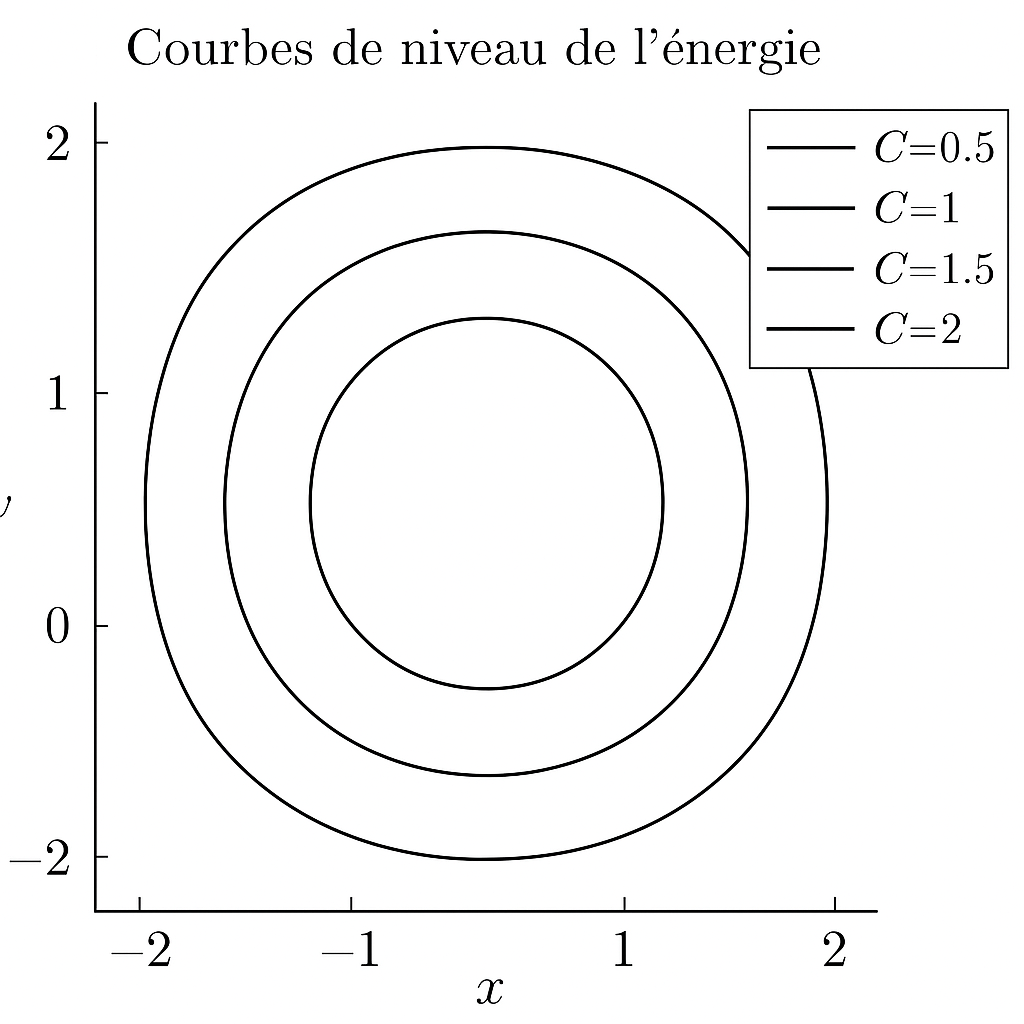
\includegraphics[scale=0.1]{./images/courbes_niveaux.png}
        \end{minipage}
        \hfill 
        \begin{minipage}{0.55\textwidth}
            Ces courbes permettent de représenter l'évolution du mouvement de l'oscillateur dans le plan. 
            Ici, plus l'énergie $C$ est élevée, plus le rayon des cercles en grand, 
            ce qui correspond à une plus grande amplitude. 

            On peut aussi les voir comme l'ensemble des orbites pour lesquelles l'énergie est égale à $C$. 
        \end{minipage}
    \end{center}
\end{example}

\begin{prop}[Orbites et Ensemble de Niveau]
    Toute orbite est incluse dans un ensemble de niveau. 
\end{prop}

Ainsi, les intégrales premières d'équations autonomes $(A)$ permettent de donner une idée de la forme des orbites formés
par les solutions de $(A)$. 

\subsubsection{Systèmes Hamiltoniens}

Il existe un cas particulier des équations autonomes appelés systèmes hamiltoniens. Ils offrent une approche plus 
simple pour l'étude des systèmes dynnamiques conservatifs, où certaines quantités sont conservées au cours du temps. 

\begin{definition}[Système Hamiltonien]
    Un système hamiltonien est une équation différentielle autonome (ou système d'équations différentielles autonomes associé) 
    pouvant être représentée par un fonction appelée \textbf{hamiltonien}. 
    Plus formellement, soit $(A) : y' = f(y)$ une équation autonome telle que $f : \Omega \longrightarrow \R^{2n}$. 
    On dit que $(A)$ est un système hamiltonien s'il existe une fonction : 
    \[ H : 
        \begin{cases}
            \Omega \overset{ \mathcal{C}^2}{\longrightarrow} \R \\ 
            (q,p) \longmapsto H(q,p) 
        \end{cases} 
        \quad \text{où } q,p \in \R^n \] 
    telle que $ \forall (q,p) \in \Omega$ on ait : 
        \[ \boxed{f(q,p) = \left( \frac{\partial H}{\partial p}, - \frac{\partial H}{\partial q} \right)  } \] 
    Cela revient donc à dire que $(A)$ peut s'écrire de la forme suivante : 
        \[ (A) : 
            \begin{cases}
                p'(t) = - \partial_q H(q,p) \\ 
                q'(t) = \partial_p H(q,p) 
            \end{cases} \] 
\end{definition}

\begin{remark}
    Tout système de dimension impaire n'est donc pas hamiltonien. 
\end{remark}

\begin{example}[Oscillateur Harmonique]
    Prenons comme exemple le cas classique d'un oscillateur harmonique gouverné par l'équation 
    différentielle : 
        \[ (A) : m x'' + kx = 0 \] 
    où : 
    \begin{itemize}
        \item $m$ est la masse de l'oscillateur 
        \item $k$ est la constante de raideur du ressort 
        \item $x(t)$ est la position de l'oscillateur à l'instant $t$. 
    \end{itemize}
    Représentons cette équation autonome sous la forme d'un système hamiltonien. 
    Posons $Y(t) = (x(t), y(t))$ on a alors $Y'(t) = (x'(t), y'(t))$. Soit la fonction suivante : 
    \[ f : 
        \begin{cases}
            \R^2 \longrightarrow \R^2 \\ 
            (x,y) \longmapsto (y, - \frac{k}{m}x)
        \end{cases} \] 
    Cela nous donne que : 
        \begin{align*}
            (A) \iff & Y'(t) = f(Y(t)) \\ 
            \iff & 
                \begin{cases}
                    x'(t) = y(t) \\ 
                    y'(t) = - \frac{k}{m} x 
                \end{cases} 
            \iff  
                \begin{cases}
                    x'(t) = \frac{1}{m} p(t) \\ 
                    p'(t) = -kx(t) 
                \end{cases}
        \end{align*}
        où $ p(t) = m x'(t)$ 
    
    Maintenant, posons : 
        \[ H : 
            \begin{cases}
                \R^2 \longrightarrow \R \\ 
                (x,p) \longmapsto \frac{p^2}{2m} + \frac{1}{2} k x^2 
            \end{cases} \] 
    $H$ est $ \mathcal{C}^\infty$ par composantes donc calculons ses dérivées partielles : 
        \[ \frac{\partial H}{\partial p} = \frac{p}{m} = x'(t) \quad \frac{\partial H}{\partial x} = k x(t) = - p'(t) \] 
    Donc $(A)$ est bien un système hamiltonien. 
\end{example}

\begin{prop}[Hamiltonien et intégrale première]
    Tout hamiltonien est une intégrale première. Autrement dit, un hamiltonien est un cas particulier d'intégrale première. 
\end{prop}

\begin{proposition}[Condition Nécessaire]
    Soit $(A) = y' = f(y)$ un système hamiltonien, alors $ \div f = 0 $. 
    En dimension 2, on a équivalence. 
\end{proposition}






    
\part[./images/probas_stats.png]{Probabilités et Statistiques}
\setcounter{chapter}{0}
% ==================================================================================================================================
% Probabilités et Statistiques

% - - - - - - - - - - - - - - - - - - - - - - - - - 
%                       TITLE
% - - - - - - - - - - - - - - - - - - - - - - - - - 


% - - - - - - - - - - - - - - - - - - - - - - - - - 
%               Chapters Inclusion
% - - - - - - - - - - - - - - - - - - - - - - - - - 

\chapter{Espaces Probabilités et Mesures}
% ==================================================================================================================================
% Introduction

\minitoc  % Affiche la table des matières pour ce chapitre




% ==================================================================================================================================
% Univers et Espace Probabilisé

\section{Univers et espace probabilisé}

Introduisons les concepts fondamentaux des probabilités, les univers et les espaces probabilisés. 

\begin{definition}[Univers]
    On appelle univers $\Omega$ pour une expérience aléatoire, l'ensemble de toutes les issues (situations finales) possibles 
    de cette expérience aléatoire. Chaque élément $ \omega \in \Omega$ représente une \textbf{issue} de cette expérience aléatoire.  
\end{definition}

\begin{example}
    \begin{itemize}
        \item Pour une expérience aléatoire de lancer de dé, il existe 6 issues possibles correspondant aux 6 faces du dé. 
        On a donc $\Omega = \{1, 2, 3, 4, 5, 6\}$. 
        \item Si on pioche un boule dans une urne contenant une boule rouge et deux boules noires, on a 
        $ \Omega = \{\text{rouge}, \text{noir}\}$. 
    \end{itemize}
\end{example}

A partir d'un univers, on peut définir la notion d'espace probabilisé. Plus complexe, la définition nécessaire les prérequis 
du cours d'intégration et de théorie de la mesure. 

\begin{definition}[Espace Probabilisé]
    Un espace probabilisé est un \textbf{triplet} $ (\Omega, \mathcal{F}, \myP)$ où :
    \begin{itemize}
        \item $\Omega$ est un univers. 
        \item $ \mathcal{F}$ est une tribu ($\sigma$-algèbre) sur $ \Omega$. 
        \item $ \myP$ est une mesure de probabilité sur $ \mathcal{F}$ (voir plus loin). 
    \end{itemize}
\end{definition}

% ==================================================================================================================================
% Évènements, Issues et Mesure de Probabilité 

\section{Évènements, Issues et Mesure de Probabilité }

\begin{definition}[Évènement]
    Soit $\Omega$ un univers. On définit un évènement de $\Omega$ comme un sous-ensemble $A \subseteq \Omega$. 
\end{definition}

\begin{remark}
    Comme définit au début, les \textbf{issues} $ \omega \in \Omega$ correspondent à des résultats élémentaires de l'expérience 
    aléatoire, à ne pas confondre avec les évènements. 
    Dans notre expérience de lancer de dé, $\{2\} \in \Omega$ est \textbf{l'issue} correspondant à "obtenir un 2" et 
    $A = \{1,2\} \subset \Omega$ est \textbf{l'évènement} correspondant à "le résultat est inférieur ou égal à 2". 
\end{remark}

Par construction, $ \mathcal{F}$ contient donc tous les évènements et issues possibles de l'expérience aléatoire. 
Elle est dont "plus complète" que $\Omega$. 

\begin{definition}[Mesure de Probabilité]
    Soit un espace probabilisé $(\Omega, \mathcal{F}, \myP)$. Une mesure de probabilité $ \myP$ 
    sur $ \mathcal{F}$ est une mesure (au sens de la théorie de la mesure) qui vérifie : 
    \begin{enumerate}
        \item $ \myP : \mathcal{F} \longrightarrow [0,1]$
        \item $ \myP(\Omega) = 1$ 
    \end{enumerate}
\end{definition}

% ==================================================================================================================================
% Variable Aléatoire

\section{Variable Aléatoire}

Pour pouvoir quantifier des calculs de probabilités ou ce que nous appellerons plus des lois, nous devons définir 
les variables aléatoires. 

\begin{definition}[Variable Aléatoire]
    Une variable aléatoire est une fonction mesurable qui associe une valeur numérique à chaque issue d'un espace probabilisé. 

    \vspace{0.5cm}

    Plus formellement, une variable aléatoire $X$ sur un espace probabilisé $(\Omega, \mathcal{F}, \myP)$ 
    est une fonction $ X : \Omega \longrightarrow \R$ telle que, pour tout ensemble $B \in \mathcal{B}_\R$ (tribu borélienne), 
    on ait $X^{-1} (B) \subset \mathcal{F}$. 
\end{definition}

La mesurabilité d'une variable aléatoire permet donc garantir que les évènements associés aux valeurs de la variable 
aléatoire sont bien mesurables par la mesure de probabilité. 

\begin{proposition}
    Maintetant que nous avons définit formellement le concept de variable aléatoire, on peut lier cette définition 
    à celle des évènements. En effet, une variable aléatoire est une fonction mesurable sur un espace probabilisé $(\Omega, \mathcal{F}, \myP)$
    telle que : 
        \[ X : \Omega \longrightarrow \R \quad \forall B \in \mathcal{B}_\R, X^{-1} (B) \subset \mathcal{F} \] 
    On peut alors caractériser un évènement $A$ comme la préimage d'un sous-ensemble de $\R$ par $X$ de la façon suivante. 
        \[ A = X^{-1}(B) \; \text{pour un certain} \; B \in \mathcal{B}_\R \] 
\end{proposition}











\chapter{Variables Aléatoires Réelles Discrètes}
% ==================================================================================================================================
% Introduction

\minitoc  % Affiche la table des matières pour ce chapitre


% ==================================================================================================================================
% Variable Aléatoire

\section{Variable Aléatoire}

\subsection{Univers et Evènement}

\begin{definition}[Univers]
    Soit $\Omega$ un ensemble. On dit que $\Omega$ est l'univers d'une expérience aléatoire s'il représente 
    l'ensemble des issues possibles pour cette expérience. 
\end{definition}

\begin{definition}[Variable Aléatoire]
    Soit $\Omega$ un univers d'une expérience aléatoire. Une variable aléatoire $X$ sur $\Omega$ 
    est une application $X : \Omega \longrightarrow \R$. On note $X(\Omega)$ l'ensemble des valeurs prises par $X$. 
\end{definition}

\begin{remark}
    Si $\Omega$ est un ensemble fini ou dénombrable, on dit que $X : \Omega \longrightarrow \R$ est une variable aléatoire réelle discrète. 
\end{remark}

\begin{example}
    Soit l'expérience aléatoire du lancer d'une pièce de monnaie non truquée. 
    On a alors $\Omega = \{\text{ Pile }, \text{ Face }\}$ et $X : \Omega \longrightarrow \R$. 
\end{example}

Une variable aléatoire associe donc des issues à des réels. Mais un événement d'une expérience aléatoire peut être 
caractérisée par plusieurs issues. Par exemple si on lance un dé à 6 faces, il y a 6 issues possibles correspondant 
à chaque face du dé. Mais on peut définir un événement telle que "le nombre obtenu est supérieur à 2". 
Dans ce cas ci, plusieurs issues de l'expérience aléatoire peuvent correspondre au même événement. 

\begin{definition}[Evènement d'une expérience aléatoire]
    Soit $X$ une variable aléatoire réelle définie sur un univers $\Omega$. 
    On appelle évènement $[X = x]$ de l'expérience aléatoire l'ensemble des issues possibles correspondant à cet évènement $x in \R$ . 
    Autrement dit :
        \[ [X = x] = \{w \in \Omega \; | \; X(\omega) = x\} = X^{-1}(x) \] 
\end{definition}

\begin{proposition}
    Soit $X$ une variable aléatoire réelle définie sur un univers $\Omega$. 
    L'ensemble des évènements possibles pour cette expérience aléatoire forme un système complet d'évènements. 
    Autrement dit : 
        \[ \sum_{x \in X(\Omega)} { \myP ([X = x])} = 1 \] 
\end{proposition}

\subsection{Loi d'une variable aléatoire}

\begin{definition}[Loi]
    Soit $X$ une variable aléatoire réelle. On appelle loi de $X$ la donnée de toutes les probabilités $ \myP(X = x)$ pour 
    tout $x \in X(\Omega)$.  
\end{definition}

Pour donner la loi d'une variable aléatoire, il faut d'abord déterminer le support de la variable aléatoire puis en suite 
calculer la probabilité de chaque issue. 
On note le résultat dans un tableau pour plus de praticité. 

\begin{example}
    Soit l'exprérience aléatoire du lancer d'un dé à 6 faces non truqué. On a :
        \[ \Omega = \{1,2,3,4,5,6\} \]
    Nous nous trouvons dans une situation d'équiprobabilité d'où :
        \[ \forall x \in X(\Omega), \quad \myP(X = x) = \frac{1}{6} \]
    D'où le tableau suivant :
    \begin{center}
        \begin{tabular}{c|c|c|c|c|c|c}
            $\Omega$ & 1 & 2 & 3 & 4 & 5 & 6 \\
            \hline 
            $ \myP(X = x)$ & $\frac{1}{6}$ & $\frac{1}{6}$ & $\frac{1}{6}$ & $\frac{1}{6}$ & $\frac{1}{6}$ & $\frac{1}{6}$ \\ 
        \end{tabular}
    \end{center}  
\end{example}

% ==================================================================================================================================
% Espérance, Variance et écart type 

\section{Espérance, Variance et écart-type}

\subsection{Espérance et propriétés}

\begin{definition}[Espérance]
    Soit $X : \Omega \longrightarrow \R$ une variable aléatoire. 
    On appelle espérance l'application $ \E : \mathcal{F}(\Omega) \longrightarrow \R $ qui calcule la moyenne de $X$ pondérée par les valeurs qu'elle prend. 
    Plus formellement :
        \[ \boxed { \E(X) = \sum_{x \in X(\Omega)} x \myP(X = x) }\] 
\end{definition}

\begin{prop}[Espérance]
    L'espérance est une fonction linéaire. Autrement dit, pour toutes variables aléatoires $X,Y$ sur  un univers $\Omega$, 
    et pour tout $a,b \in \R$, on a :
        \[ \E(X+Y) = \E(X) + \E(Y) \quad \E(aX + b) = a\E(X) + b \]
\end{prop}

Lors d'une expérience aléatoire, par exemple un jeu d'argent l'espérance représente le gain moyen d'un joueur par partie 
s'il joue un grand nombre de fois. Son signe permet de savoir si le jeu est dit équitable (autant de chances de gagner que 
de perdre). 

\vspace{0.3cm}

Il peut souvent arriver que l'on veuille appliquer une fonction à notre variable aléatoire. 
Un théorème nous permet alors simplement de calculer l'espérance de cette "nouvelle" variable aléatoire. 

\begin{theorem}[Transfert]
    Soit $X$ une variable aléatoire sur un univers $\Omega$ et $g : \R \longrightarrow \R$ une application. 
    L'espérance de la variable aléatoire $g(X) : \Omega \longrightarrow \R$ est l'application $ \E(g(X)) : \mathcal{F}(\Omega) \longrightarrow \R$ 
    telle que : 
        \[ \boxed{ \E(g(X)) = \sum_{x \in X(\Omega)} g(x) \myP(X = x) } \]  
\end{theorem}

\subsection{Variance et écart-type}

\begin{definition}[Variance et écart-type]
    Soit $X$ une variable aléatoire sur un univers $\Omega$. On appelle variance l'application 
    $\V : \mathcal{F}(\Omega) \longrightarrow \R$ telle que :
        \[ \boxed { \V(X) = \sum_{x \in X(\Omega)} (x - \E(X))^2 \myP(X = x) } \]
    De même, on appelle écart type l'application $ \sigma : \mathcal{F}(\Omega) \longrightarrow \R$ telle que : 
        \[ \boxed{ \sigma(X) = \sqrt{\V(X)} } \]  
\end{definition}

La variance permet de mesurer la dispersion de la variable aléatoire autour de son espérance. 

\begin{remark}
    Les notions d'espérance, variance et écart-type sont définies par des sommes potentiellement infinies. 
    Il se peut donc que dans le cas de variables aléatoires définies sur des univers infinies, leur espérance, 
    variance et écart-type n'existent pas. Une étude de convergence de la somme est donc judicieuse. 

    En revanche pour les variables aléatoires finies (definies sur un univers fini) ces notions sont toujours 
    bien définies. 
\end{remark}

\begin{theorem}[Formule de König-Huygens]
    Soit $X$ une variable aléatoire sur un univers $\Omega$ fini. On a alors : 
        \[ \boxed{ \V(X) = \E(X^2) - \E(X)^2 } \]
\end{theorem}

\begin{remark}
    Le calcul de la variance d'une variable aléatoire réelle finie est donc assez facile quand on le met en relation 
    avec la formule de König-Huygens et la formule du transfert...
\end{remark}

A partir de toutes ces formules, on peut en déduire quelques propriétés sympatiques sur la variance :

\begin{prop}[Variance]
    Soit $X$ une variable aléatoire finie et $a,b \in \R$, on a :
        \[ \V(aX+b) = a^2 \V(X) \quad \V(X + b) = \V(X) \]
    La variance est donc assez similaire à une forme quadratique et est invariante par translation. 
\end{prop}

\begin{theorem}[Inégalité de Markov]
    Si $X$ est une variable aléatoire réelle discrète \textbf{positive} ou nulle sur $\Omega$ d'espérance $\E(X)$, alors :
        \[ \forall a \in ]0, + \infty [ \quad P(X \geqslant a) \leqslant \dfrac{\E(X)}{a} \]
    En l'appliquant à la variable aléatoire $(X - \E(X))^2$ et en remarquant que son espérance vaut $\sigma^2$ et l'égalité des événements $|X - \E(X)| \geqslant \alpha$ et $(X - \E(X))^2 \geqslant \alpha^2 $ on obtient :
        \[ \forall \alpha > 0, \quad P(|X - \E(X)| \geqslant \alpha) \leqslant \dfrac{\sigma^2}{\alpha^2}\]
\end{theorem}

% ==================================================================================================================================
% Principales Lois

\section{Principales Lois}

Abordons en détail maintenant quelques lois usuelles à connaître sur le bout des doigts. 
Ces lois permettent de modéliser la plupart des expériences aléatoires. 

\subsection{Loi Uniforme}

\begin{definition}[Loi Uniforme]
    Soit $n \in \N^*$. On dit qu'un variable aléatoire $X$ suit une \textbf{loi uniforme} sur $ \llbracket 1, n \rrbracket $ 
    lorsque son support est $X(\Omega) = \llbracket 1, n \rrbracket $ et chaque issue a la même probabilité de se produire. 
    Autrement dit : 
        \[ \forall x \in \llbracket 1, n \rrbracket, \quad P(X = x) = \frac{1}{n} \]
    On note alors $X \sim \mathcal{U}(\llbracket 1, n \rrbracket)$. 
\end{definition}

\begin{proposition}
    Soit $X \sim \mathcal{U}(\llbracket 1, n \rrbracket)$ alors l'espérance et la variance de $X$ sont de la forme : 
        \[ \E(X) = \frac{n+1}{2} \quad \text{et} \quad \V(X) = \frac{n^2-1}{12}  \] 
\end{proposition}

\subsection{Loi de Bernouilli}

\begin{definition}[Loi de Bernouilli]
    Une variable aléatoire $X$ suit une \textbf{loi de Bernoulli} de paramètre $p \in ]0,1[$ si il n'existe que deux issues 
    possibles $X(\Omega) = \{ 0,1 \}$ telles que : 
        \[ \myP(X = 1) = p \quad \text{et} \quad \myP(X = 0) = 1 - p \] 
    On note alors $X \sim \mathcal{B}(p)$.  
\end{definition}

\begin{proposition}
    Soit $X \sim \mathcal{B}(p)$ alors l'espérance et la variance de $X$ sont de la forme :
        \[ \E(X) = p \quad \text{et} \quad \V(X) = p(1-p)  \] 
\end{proposition}

\subsection{Loi Binomiale}

L'expérience aléatoire consistant à répéter $n \in \N$ fois une expérience de Bernoulli de paramètre $ p \in ]0,1[$
de {manière indépendante} est appelée \textbf{schéma de Bernoulli} de paramètres $n$ et $p$. 

\begin{definition}[Loi Binomiale]
    La variable aléatoire $X$ égale au \textbf{nombre de succès} d'un schéma de Bernoulli suit une {loi binomiale} 
    de paramètres $n$ et $p$. 

    On note alors $X \sim \mathcal{B}(n,p)$. 
\end{definition}

\begin{proposition}
    Soit $X \sim \mathcal{B}(n,p)$. On a alors $X(\Omega) = \llbracket 0, n \rrbracket$ et pour tout $k \in \N$ tel que 
    $0 \leqslant k \leqslant n $, {la probabilité d'obtenir $k$ succès} est donnée par :
        \[ \myP(X = k) = \binom{k}{n} \times p^k \times (1-p)^{n-k}  \] 
\end{proposition}

\begin{proposition}
    Soit $X \sim \mathcal{B}(n,p)$ alors l'espérance et la variance de $X$ sont de la forme :
        \[ \E(X) = np \quad \text{et} \quad \V(X) = np(1-p)  \] 
\end{proposition}

\newpage
\subsection{Loi géométrique}

\begin{definition}[Loi géométrique]
    Une variable aléatoire $X$ suit une loi géométrique de paramètre $p \in ]0,1[$ lorsque $X(\Omega) = \N^*$ et que 
        \[ \forall k \in \N^*, \quad \myP(X = k) = p(1-p)^{k-1}  \] 
    On note alors $X \sim \mathcal{G}(p)$. 
\end{definition}

Une loi géométrique représente le temps d'attendre du premier succès d'un espérience de Bernoulli. 
Autrement dit X est le rang de l'épreuve ayant mené au premier succès. 

\begin{proposition}
    Soit $X \sim \mathcal{G}(p)$ où $p \in ]0,1[$ l'espérance et la variance de $X$ sont de la forme :
        \[ \E(X) = \frac{1}{p} \quad \text{et} \quad \V(X) = \frac{1-p}{p^2} \] 
\end{proposition}

\subsection{Loi de Poisson}

\begin{definition}[Loi de Poisson]
    Une variable aléatoire $X$ suit une loi de Poisson de paramètre $\lambda > 0$ lorsque $X(\Omega) = \N$ et 
        \[ \forall k \in \N, \quad P(X = k) = e^{- \lambda} \times \frac{\lambda^k}{k!} \]  
    On note alors $ X \sim \mathcal{P}(\lambda)$. 
\end{definition}

Une loi de poisson représente le nombre moyen d'évènements produits au cours d'un intervalle de temps donné ou d'une quantité 
donnée. Par exemple, elle peut modéliser le nombre moyen de voitures qui sont passées par un péage sur une journée ou le nombre 
moyen de fautes de frappes produits sur une page de texte. 

\begin{proposition}
    Soit $ X \sim \mathcal{P}(\lambda)$ alors l'espérance et la variance de $X$ sont de la forme :
        \[ \E(X) = \lambda \quad \text{et} \quad \V(X) = \lambda  \] 
\end{proposition}



\chapter{Variables Aléatoires Continues}
% ==================================================================================================================================
% Introduction

\minitoc  % Affiche la table des matières pour ce chapitre


On s'intéresse maintenant à des variables aléatoires qui prennent des valeurs réelles mais pas forcément en nombre fini ou dénombrable.
Il est donc nécessaire de definir une probabilité sur $\R$ telle que la probabilité des singletons soit nulle.

Pour cela, nous allons très fortement nous appuyer sur l'intégrale de Lebesgue et la théorie de la mesure. 

% ==================================================================================================================================
% Tribu Borélienne et Mesure 

\section{Tribu Borélienne et Mesure}

\subsection{Borélien vous dites ?}

\begin{definition}[Tribu]
    Soit $X$ un ensemble. Une tribu sur $X$ est une partie $ \mathcal{B} \subseteq \mathcal{P}(X)$ telle que :
    \begin{enumerate}[label=\roman*)]
        \item $\emptyset \in \mathcal{B}$ 
        \item $ \mathcal{B}$ est stable par complémentaire 
        \item $ \mathcal{B}$ est stable par union dénombrable
    \end{enumerate}
    Un élément de $ \mathcal{B}$ est appelé \textbf{partie mesurable}. 
    On appelle le couple $(X, \mathcal{B})$ un espace mesurable. 
\end{definition}

\begin{remark}
    Si on prend $X = \R$, on appelle alors sa tribu la \textbf{tribu borélienne}. 
    C'est la plus petite tribu contenant tous les ouverts de $\R$. 
    On la note $ \mathcal{B}_\R$. 
\end{remark}

\begin{proposition}
    Soit $A$ un ensemble et $X$ un ensemble de parties de $A$. Il existe une plus petite tribu sur 
    $A$ qui contienne $X$. On l'appelle \textbf{tribu engendrée} par $X$, notée $\sigma (C)$.

    On définit ainsi la \textbf{tribu borélienne} sur $\R$ la tribu engendrée par les intervalles ouverts de $\R$. 
    Les éléments de la tribu sont appelés les boréliens.
\end{proposition}

\newpage 
\subsection{Mesure}

\begin{definition}[Mesure]
    Soit $X$ un ensemble muni d'une tribu $ \mathcal{B}$. On appelle mesure sur $ \mathcal{B}$ toute application 
        \[ \mu : \mathcal{B} \longrightarrow \overline{R_+} \] 
    telle que : 
    \begin{enumerate}[label=\roman*)]
        \item $\mu (\emptyset) = 0 $
        \item $ \forall (A_n)_{n \in \N}$ suite de parties mesurables deux à deux disjointes :
            \[ \mu \left( \bigcup_{n \in \N} A_n \right) = \sum_{n \in N} \mu (A_n) \] 
    \end{enumerate}
    On appelle le triplet $(X, \mathcal{B}, \mu)$ un espace mesuré. 
\end{definition}

\begin{theorem}[Mesure de Lebesgue]
    Il existe une unique mesure $\lambda$ sur $(\R, \mathcal{B}_\R)$ appelée mesure de Lebesgue telle que : 
        \[ \lambda : 
            \begin{cases}
                \mathcal{B}_\R \longrightarrow \overline{\R_+} \\ 
                ]a,b] \longmapsto b-a 
            \end{cases}
        \] 
    On a $\lambda(\R) = \infty$. 
\end{theorem}

\subsection{Partie Négligeable et propriété vraie presque partout}

\begin{definition}[Partie Négligeable]
    Soit $(X, \mathcal{B},\mu)$ un espace mesuré. On appelle partie négligeable de $X$ toute partie $A$ mesurable telle que 
    $\mu(A) = 0$. 
\end{definition}

\begin{definition}[Propriété vraie presque partout]
    Soit $(X, \mathcal{B},\mu)$ un espace mesuré. Soient $A$ une partie mesurable de $X$ et $ \mathcal{P}(A)$ une propriété sur $A$. 
    On dit que $ \mathcal{P}(A)$ est vraie presque partout ssi :
        \[ \mu ( \{ x \in A \; | \; \lnot \mathcal{P}(A) \} ) = 0 \] 
    Autrement dit, une propriété sur une partie mesurable est vraie presque partout ssi l'ensemble des points où elle est fausse 
    est négligeable. 
\end{definition}

% ==================================================================================================================================
% Variables Aléatoires Continues

\section{Variables aléatoires continues}

\begin{definition}[Espace Probabilisé]
    Soit une expérience aléatoire. On appelle le triplet $(\Omega, \mathcal{F}, \myP)$ un espace probabilisé si :
    \begin{enumerate}[label=\roman*)]
        \item $\Omega$ est un ensemble d'évènements possibles 
        \item $ \mathcal{F}$ est une tribu des évènements mesurables. 
        \item $\myP : \mathcal{F} \longrightarrow [0,1]$ est une mesure définie sur l'espace mesurable $(\Omega, \mathcal{F})$. 
    \end{enumerate}
    On appelle $\myP$ une mesure de probabilité sur $(\Omega, \mathcal{F})$. 
\end{definition}

\begin{definition}[Variable Aléatoire]
    Soit $(\Omega, \mathcal{F}, \myP)$ un espace probabilisé et $(\R, \mathcal{B}_\R)$ un espace mesuable. 
    Une variable aléatoire de $\Omega$ vers $\R$ toute fonction mesurable $X : \Omega \longrightarrow \R$.  
\end{definition}

\begin{definition}[Loi de probabilité]
    Soit $(\Omega, \mathcal{F},\myP)$ un espace probabilisé et $X$ une variable aléatoire sur $\Omega$. 
    La loi de $X$ est la mesure image de $ \myP$ par X. Autrement dit :
        \[ \forall B \in \mathcal{F}, \quad \myP(X \in B) = \myP( \{ \omega \in \Omega \; | \; X(\omega) \in \Omega \} ) \] 
    
\end{definition}




















\vspace{5cm}

\begin{definition}[Fonction de répartition]
    On appelle fonction de répartition de la variable aléatoire $X$ la fonction 
    \[ F_X : 
        \begin{cases}
            \R &\longrightarrow [0, 1] \\
            a &\longmapsto P(X \in ]- \infty, a[)
        \end{cases}
    \]
    $F_X$ est une fonction croissante admettant la limite $0$ en $- \infty$ et la limite $1$ en $+ \infty$ et elle est continue à droite. 
\end{definition}

\begin{definition}[Continuité d'une variable aléatoire réelle]
Une variable aléatoire réelle $X$ est dite continue si il existe une fonction $F_X$ intégrable sur $\R$ positive ou nulle et continue par morceaux 
    et telle que :
    \[ \forall x \in \R, \quad \int_{- \infty}^{X} f_X(t) dt = F_X(X) \]
    $f_X$ est alors la \textbf{densité} de la variable $X$.
\end{definition}


\section*{Principales Lois}

\begin{definition}[Loi uniforme]
    La variable aléatoire $X$ continue dont la densité est constante sur un intervalle borné $I$ et nulle en dehors est appelée la loi uniforme sur l'intervalle $I$ notée $\mathcal{U}(I)$.
    Ainsi, on a :
        \[ I = [a, b] \subset \R, \quad f_X(t) = 
            \begin{cases}
                0 \text{ si } & \text{ t } \not \in [a, b] \\
                \dfrac{1}{b-a} & \text{ si } t \in [a, b]
            \end{cases}
            \; \text{ et } \; 
            F_X(x) = 
            \begin{cases}
                0 & \text{ si } x \leq a \\
                \dfrac{x - a}{b - b} & \text{ si } a \leq x \leq b \\
                1 & \text{ si } x \geq b 
            \end{cases}
        \]    
\end{definition}


\begin{definition}[Loi Normale]
    La loi normale (ou gaussienne ou de Laplace-Gauss) notée $\mathcal{N}(\mu, \sigma^2)$ de moyenne $\mu$ et d'écart-type $\sigma$ est la loi continue sur $\R$ de densité :
        \[ f_X(x) = \dfrac{1}{\sigma \sqrt{2 \pi}} e^{- \dfrac{(x - \mu)^2}{2 \sigma^2}}\]
    de fonction de répartition :
        \[ F_{\mu, \sigma^2}(a) = \int_{ -\infty}^{a} \dfrac{1}{\sigma \sqrt{2 \pi}} e^{- \dfrac{(x - \mu)^2}{2 \sigma^2}} \]
\end{definition}

\begin{definition}[Loi exponentielle]
    La loi exponentielle $\mathcal{E}(\lambda)$ de paramètre $\lambda > 0$ est la loi de densité nulle sur $\R_{-}$ et égale à $\lambda e^{-\lambda x}$ sur $\R_+$.
    Sa fonction de répartition est la suivante :
    \[ F(t) = 
        \begin{cases}
            0 \text{ si } t \leq 0 \\
            {0}^{t} \lambda e^{-\lambda x} dx = [- e^{- \lambda x} ]_0^t = 1 - e^{- \lambda t} \; \text{ si } t \geq 0
        \end{cases}
    \]
\end{definition}


\section*{Propriétés des variables aléatoires continues}

\begin{definition}[Espérance]
    Soit $X$ une variable aléatoire continue réelle absolument continue de densité $f_X$.
    On appelle espérance de $X$ le nombre 
        \[ E(X) = \int_{\R} t f_X(t) dt \]
    Si cette espérance n'est pas absolument convergente, on dit que $X$ n'a pas d'espérance.
\end{definition}

\begin{theorem}[Formule de Transfert]
    Soit $X$ est une variable aléatoire réelle absolument continue de densité $f_X$ et si $\varphi$ est une fonction $\mathcal{C}^1$, alors $\varphi(X)$ est une variable aléatoire réelle.
    Si elle admet un espérance, on a alors :
        \[ E(\varphi(X)) = \int_{\R} \varphi (t)f_X(t) dt\]
\end{theorem}

\begin{definition}[Variance]
    Soit $X$ une variable aléatoire admettant une espérance. La variance de $X$ est le nombre :
        \[ V(X) = E((E - E(X))^2) = \int_{\R} (t - E(X))^2 f(t) dt \]
    Toujours comme chez les variables aléatoires réelles discrètes, l'acrt type de $X$ est la racine carrée de $V(X)$ si $V(X)$ existe.
\end{definition}

% \begin{theorem}[Koenig-Huyghens]
%     \[ V(X) = E(X^2) - E(X)^2 \]
% \end{theorem}



\section*{Lois conjointes continues}

\begin{definition}[Vecteur Aléatoire]
    Une vecteur aléatoire à $n$ composantes est une al=pplication $V$ d'un espace probabilisé $(\Omega, \mathcal{A}, P)$ dans $\R^n$ telle que l'image réciproque $V^{-1}(B)$ de tout borélien de $\R^n$ soit un élément de la tribu de $\Omega$.
\end{definition}

\begin{theorem}[Fubini]
    Si $ f : \R^2 \rightarrow \R $ est intégrable sur $[a, b] \times [c, d]$ alors pour presque tout $x \in [a, b]$, la fonction partielle $ y \mapsto f(x, y)$ est intégrable sur $[c, d]$ et 
        \[ \iint_{[a, b] \times [c, d]} f(x, y) dx \; dy = \int_{a}^{b} \left( \int_{c}^{d} f(x, y) dy \right) dx \]
\end{theorem}

\begin{definition}[Densité Conjointe]
    Soit $ f : \R^2 \rightarrow \R $ une application intégrable telle que $f \geq 0$ et 
        \[ \iint_{\R^2} f(x, y) dx \; dy = 1 \]
    Alors la loi $\mathcal{L}(X, Y)$ du couple $(X, Y)$ est absolument continue de densité conjointe $f$ si, pour tout borélien $B$, on a :
        \[ P((X, Y) \in B) = \iint_B f(x, y) dx \; dy \]
\end{definition}











\section*{Démonstrations}

- intersection quelconque de tribu est une tribu
- limite et continuité de la fonction de répartition





\chapter{Vecteurs Aléatoires}
\input{subjects/Probas-Stats/chapitres/chapitre3_Vecteurs_Aléatoires.tex}

\chapter{Fonctions Génératrices}
% ==================================================================================================================================
% Introduction

\minitoc  % Affiche la table des matières pour ce chapitre

\section*{Définition Générale}

On considère une variable aléatoire discrète entière positive non nulle $X$ qui prend ses valeurs dans $\N$ et pour tout $n$ dans $\N$ on pose 
$p_n = P(X = n)$, on a donc, d'après la définition d'une probabilité $ \sum_{n=0}^{\infty} p_n = 1 $

\begin{definition}[Fonction Génératrice]
    On appelle fonction génératrice de $X$ la fonction :
        \[ \boxed{ g_X(z) = \sum_{n=0}^{\infty} P(X = n) z^n} \] 
    C'est une série entière de la variable $z \in \C$.    
\end{definition}

\begin{remark}
    Le rayon de convergence cette série est \underline{supérieur} à $1$.
\end{remark}

\section*{Propriétés}

\begin{itemize}
    \item $g_X$ est continue sur $ \overline{D(0, 1)}$ et $\mathcal{C}^\infty$ sur $D(0, 1)$.
    \item pour $|z| > 1$ on a $g_X(z) = E(z^X)$
    \item la fonction génératrice caractérise la loi 
        \[ \text{i.e. } g_X = g_Y \text{ sur un voisinnage de 0} \Longrightarrow \mathcal{L}(X = \mathcal{L}(Y) \] 
    \item si $E(X)$ existe alors $E(X) = g_X(1)$ 
    \item si $E(X^k), k \in \N$ existe alors $g_X^{(k)}(z) = E(X(X-1)(X-2) \dots (X - k + 1))$ 
        
        En particulier, si $E(X^2)$ existe, alors 
            \[ g_X^{\prime \prime}(1) = E(X(X-1)) = E(X^2) - E(X) \] 
        Donc $ V(X) = g_X^{\prime \prime}(1) + g_X^{\prime}(1) - (g_X^{\prime}(1))^2 $
\end{itemize}


\section*{Somme de variables aléatoires entières positives indépendantes}

\begin{theorem}
    Si $X$ et $Y$ sont indépendantes, alors 
        \[ g_{X + Y} = g_X g_Y \] 
\end{theorem}

\begin{proof}
    On a :
        \[ g_X(z) = \sum_{n\in \N} p_n z^n, \quad g_Y(z) = \sum_{n \in \N} q_n z^n, \quad g_{X+Y}(z) = \sum_{n \in \N} r_n z^n \] 
    D'après la formule des probabilités totales :
        \[ r_n = P(X + Y = n) = \sum_{k = 0}^{n} P(X = k) P(Y = n-k) = \sum_{k=0}^{n} p_k q_{n_k} \]
    et 
    \begin{align*}
        g_{X +Y}(z) &= \sum_{n = 0}^{\infty} \sum_{k = 0}^{n} p_k q_{n-k} z^n = \sum_{n = 0}^{\infty} \sum_{k = 0}^{n} p_k q_{n-k} z^k z^{n-k} \\
        &= \Biggl( \sum_{i = 0}^{\infty} p_i z^i \Biggr) \Biggl( \sum_{j = 0}^{\infty} q_j z^j \Biggr) \\
        &= g_X g_Y
    \end{align*}
   
\end{proof}


\chapter{Convergences}
% ==================================================================================================================================
% Introduction

\minitoc  % Affiche la table des matières pour ce chapitre

Soit $(X_n)_{n \in \N}$ une suite de variables aléatoires indépendantes suivant la même loi.
On considère $Y_n = \frac{1}{n} (\sum_{k=1}^{n} X_k)$. On suppose que $V(X_n)$ est finie.

    \[ E(Y_n) = \frac{1}{n} \sum_{k=1}^{n} E(X_k) = E(X_n) \] 
et 
    \[ 
        \begin{aligned}
            V(Y_n) &= V \left( \frac{1}{n} \sum_{k=1}^{n} X_k \right)  = \frac{1}{n^2} V \left( \sum_{k=1}^{n} X_k \right)  \\
            &= \frac{1}{n^2} \sum_{k=1}^{n} V(X_k) = \frac{1}{n} V(X_n)
        \end{aligned}
     \] 
on applique ensuite l'inégalité de Bienaymé-Tchebychev à $(Y_n)$
        \[ \boxed{ P(|Y_n - E(X_1) \geq b) \leq \frac{V(Y_n)}{b^2} = \frac{1}{n} \frac{V(X_0)}{b^2} \underset{n \to + \infty}{\longrightarrow} 0 } \] 



\section*{Convergence en probabilités}

Soit $(Z_n)_{n \in \N}$ une suite de variables aléatoires sur un même espace $\Omega$. Soit $Z_\infty$ une variable sur $\Omega$. 

\begin{definition}[Convergence en Probabilités]
    On dit que la suite $(Z_n)_{n \in \N}$ converge en probabilité vers $Z_\infty$ si 
        \[ \forall \varepsilon > 0, \quad \boxed{ P(|Z_n - Z_\infty| \geq \varepsilon) \underset{n \to + \infty}{\longrightarrow} 0} \]
    On notera : $ Z_n \stackrel{P}{\longrightarrow} Z_\infty $
\end{definition}

\begin{remark}
    La loi faible des grands nombres affirme que $(Y_n)_{n \in \N}$ converge en probabilité vers la loi quasi-certaine $E(X_1)$.
\end{remark}


\section*{Convergence presque-sûre}

Si on considère nos $Z_n$ comme des fonctions sur $\Omega$ à valeurs dans $\R$, on pourrait essayer de voir à quoi correspondrait la convergence simple.

\begin{comment}
    \begin{example}
        Soit $(\omega_k)_{k \in \N} \in \Omega = \{0, 1\}^\N$. Posons $X_n = \omega_n$.
        Sur $\Omega$ on a la probabilité "définie" par le fait que si 
            \[ A_{\{ \varepsilon_0, \dots , \varepsilon \}} = \Bigl\{ \omega \in \Omega, \omega_i = \varepsilon_i, \forall i \in \{0, 1, \dots, n\} \Bigl\} \]
        alors 
            \[ \forall \varepsilon \in \{0, 1\}, \Theta \in ]0, 1[,  \quad P(A) = \Theta ^{\sum_{i=0}^{n} \varepsilon i} \bigl( 1 - \Theta \bigr)^{\sum_{i=0}^{n} (1- \varepsilon_i)} \] 
        Donc 
    \end{example}
\end{comment}

\begin{definition}[Convergence presque-sûre]
    Soit $\Omega$ un espace probabilisé, soit $(Z_n)_{n \in \N}$ une suite de variables aléatoires sur $\Omega$.
    Soit $Z_\infty$ une variable aléatoire sur $\Omega$. On dit que $(Z_n)$ converge presque sûrement vers $Z_\infty$ si 
        \[ P(Z_n(\omega) \longrightarrow (Z_n(\omega))) = 1 \] 
    i.e. l'ensemble des $\omega \in \Omega$ pour lesquels il n'y a pas de convergence est un ensemble négligeable.    
\end{definition}

\begin{theorem}[Loi forte des grands nombres]
    Soient $(X_n)_{n \in \N}$ la suite de variables aléatoires réelles continues, indépendantes et suivant la même loi. 
    Supposons que nous connaissons son espérance $(E(X_i))$ et sa variance $V(X_1)$.
    Alors $Y_n = \frac{1}{n} \sum_{k=1}^{n} X_k$ converge presque sûrement vers la constante $E(X_1)$.    
\end{theorem}




\section*{Convergence en moyenne quadratique}

\begin{definition}
    Soit $(Z_n)_{n \in \N}$ une suite de variables aléatoires réelles sur un même espace probabilisé $\Omega$.
    Soit $Z_\infty$ une variable aléatoire réelle sur $\Omega$. On dit que $(Z_n)$ converge en moyenne quadratique vers $Z_\infty$ si 
        \[ E((Z_n - Z_\infty)^2) \underset{n \to \infty}{\longrightarrow} 0 \] 
    On note $Z_n \stackrel{mq}{\longrightarrow} Z_\infty $
\end{definition}

\begin{example}
    Dans le contexte de la loi des grands nombres on avait $E(Y_n) = E(X_1)$ et $V(Y_n) = \frac{1}{n} V(X_1) \underset{n \to + \infty}{\longrightarrow} 0$ donc on avait une convergence en moyenne quadratique.
\end{example}

\begin{remark}
    Sur l'ensemble des variables aléatoires sur $\Omega$, la variance est une forme quadratique positive dont la forme bilinéaire symétrique associée est la covariance.
    La convergence en moyenne quadratique esr la convergence pour cette "norme".
\end{remark}

\begin{proposition}
    Si la suite $(X_n)_{n \in \N}$ converge en moyenne cubique vers $X$ alors :
        \[  
            \left.
            \begin{aligned}
                \lim_{n \to \infty} E(X_n) &= E(X) \\
                \lim_{n \to + \infty} E({X_n}^2) &= E(X^2)
            \end{aligned}
            \right\}
            \Longrightarrow
            \lim_{n \to + \infty} V(X_n) = V(X)
        \]
\end{proposition}

\begin{proof}
    $X_n$ et $X$ admettent une variance et $E((X_n - X)^2) \underset{n \to \infty}{\longrightarrow} 0$, d'après la seconde inégalité triangulaire, on a
        \[ | \sqrt{E({X_n}^2)} - \sqrt{E(X^2)} | \leq \sqrt{E((X_n - X)^2)} \underset{n \to \infty}{\longrightarrow} 0 \] 
    pour la forme quadratique positive $(X, Y) \mapsto E(X, Y) = <X, Y> $. C'est une forme linéaire symétrique positive qui respecte l'inégalité triangulaire.
    D'où $\sqrt{E({X_n}^2) - E(X^2)} \underset{n \to \infty}{\longrightarrow} 0 $ donc $E({X_n}^2) \underset{n \to \infty}{\longrightarrow} E(X^2)$
\end{proof}

\begin{remark}[Variance et Cauchy-Schwarz]
    D'après l'inégalité de Cauchy-Schwarz :
    \[
        \begin{aligned}
            |E(X_n) - E(X)| &= |E(X_n - X)| = |<X_n -X, 1>| \\
            & \leq \sqrt{< X_n - X, X_n -X>} \sqrt{<1, 1>} \\
            &= \sqrt{E((X_n - X)^2)} \underset{n \to \infty}{\longrightarrow} 0 
        \end{aligned}
    \] 
    Donc $|E(X_n - E(X))| \underset{n \to \infty}{\longrightarrow} 0 $ par encadrement.
    Or $V(X_n) = E({X_n}^2) - E(X_n)^2$ donc $V(X_n) \underset{n \to \infty}{\longrightarrow} 0 $
\end{remark}

\begin{corollary}[Critère de convergence quadratique]
    $(X_n)_{n \in \N}$ converge en moyenne quadratique vers la variable certaine $a \in \R$ ssi
        \[ E(X_n) \underset{n \to \infty}{\longrightarrow} a \quad \text{et} \quad V(X_n) \underset{n \to \infty}{\longrightarrow} 0 \] 
\end{corollary}



\chapter{Lois Conjointes}
\input{subjects/Probas-Stats/chapitres/chapitre6_Lois_Conjointes.tex}

\chapter{Estimation Ponctuelle}
% ==================================================================================================================================
% Introduction

\minitoc  % Affiche la table des matières pour ce chapitre

\begin{quote}
    La statistique ou les statistiques1 est la discipline qui étudie des phénomènes à 
    travers la collecte de données, leur traitement, leur analyse, l'interprétation des 
    résultats et leur présentation afin de rendre ces données compréhensibles par tous. 
    C'est à la fois une branche des mathématiques appliquées2, une méthode et un ensemble de techniques. 

    \hfill --- \href{https://fr.wikipedia.org/wiki/Statistique}{Source : Wikipédia}
\end{quote}

En pratique, lorsque l'on essaye de déterminer des caractéristiques d'une population, 
on réunit celle-ci et on "compte" le nombre d'occurences des propriétés qui nous intéressent. 
Une fois fait, il suffit d'appliquer quelques formules pour déterminer quelques caractéristiques 
de la population. 

Cependant, lorsque l'on souhaite, par exemple savoir la proportion de Français droitier. Il faudrait donc 
mettre en place à très grande échelle un sondage pour que chaque Français dise s'il est droitier ou gaucher. 
Outre le fait que l'expérience n'ait aucun intérêt, elle semble très compliqué à mettre en place. 
Il faudrait donc sonder seulement une partir des Français (on appelera cela un échantillon) et à partir du 
résultat obtenu, en déduire le résultat pour l'ensemble des Français. On appelle ces processus l'échantillonnage 
et l'estimation d'un paramètre à partir d'un échantillon (ici une proportion). 

% ==================================================================================================================================
% Echantillonnage 

\section{Echantillonnage}

\subsection{Généralités et définitions}

La théorie de l'échantillonnage a pour but de déterminer la distribution d'une caractéristique $X$ dans une 
population $P$ à partir de l'étude d'un sous-ensemble de cette population. On appelle ce sous-ensemble un 
échantillon de la population. 

\begin{definition}[Echantillonnage Simple]
    On appelle échantillonnage simple le procédé qui consiste, à partir d'une population $P$ de 
    choisir au hasard $n$ individus de la population de manière aléatoire. 
    Ainsi chaque individu a la même probabilité d'être sélectionné pour l'échantillonnage. 
\end{definition}

Plus formellement, nous allons représenter un échantillon par des variables aléatoires suivant une 
loi prédéfinie $X$ correspondant au paramètre recherché. Ainsi, un échantillon de taille $n$ d'une population sera un $n$-uplet de variables aléatoires 
    \[ (X_1, \dots, X_n) \]
indépendantes et de même loi que $X$. 

\begin{definition}[Echantillon et réalisation]
    Soit $X$ une variable aléatoire sur un espace probabilisé $(\Omega, \mathcal{F}, \myP)$. 
    Un échantillon de $X$ de taille $n \in \N$ est une $n$-uplet de variables aléatoires 
    $(X_1, \dots, X_n)$ iid de même loi que $X$ de paramètre $\theta \in \R$. 

    \vspace{0.3cm}

    Une réalisation de cet échantillonage est un $n$-uplets de réel $(x_1, \dots, x_n)$ tels que 
    $ \forall i \in \llbracket 1, n \rrbracket, \; X_i(\omega) = x_i$ où $ \omega \in \Omega$. 
\end{definition}

\begin{remark}
    On appellera $X$ la \textbf{loi mère}. 
\end{remark}

\begin{example}
    Ici un exemple du cours
\end{example}

\subsection{Moyenne et Variance Empirique}

\begin{definition}[Statistique]
    Considérons un échantillon d'une population $(X_1, \dots, X_n)$ sur un espace probabilisé 
    $(\Omega, \myP )$ tels que: 
        \[ \forall i \in \llbracket 1, n \rrbracket, \quad X_i : \Omega \longrightarrow E \]
    où $E \subseteq \R$ généralement.  
    Une statistique est une fonction qui associe une valeur à chaque réalisation de l'échantillon telle que: 
        \[ T : E^n \longrightarrow Im(T) \subseteq \K \] 
\end{definition}

\subsection{Moyenne et loi normale}

\begin{definition}[Moyenne Empirique]
    Soit  $(X_1, \dots, X_n)$ un échantillon d'une population sur un espace probabilisé. 
    On appelle \textbf{moyenne empirique} de l'échantillon la moyenne arithmétique des variables de l'échantillon. 
    On la note $\overline{X}_n$ telle que: 
        \[ \overline{X}_n := \frac{1}{n} \sum_{i=0}^{n} X_i \]
\end{definition}

\begin{example}
    Pour un échantillon $(X_1, \dots, X_n)$, la moyenne empirique est une statistique de cet échantillon. 
\end{example}

\begin{proposition}
    Soit $X_1, \dots, X_n$ un échantillon élatoire de taille $n$ de variables iid tiré 
    d'une distribution $X$ d'espérance $\mu$ et de variance $\sigma^2$. On a les propriétés suivantes: 
        \[ \E(\overline{X}_n) = \mu \quad \V(\overline{X}_n) = \frac{\sigma^2}{n} \]  
\end{proposition}

\begin{itemize}
    \item L'espérance de la moyenne empirique reste égale à 
    l'espérance de la variable aléatoire sous-jacente, car chaque observation apporte une estimation de $\mu$.
    \item La variance de la moyenne empirique est plus petite que celle de la variable aléatoire initiale, 
    et elle diminue avec la taille de l'échantillon $n$. 
    Cela reflète le fait que la moyenne empirique devient plus précise quand on augmente le nombre d'observations. 
\end{itemize}

\newpage 

\begin{theorem}[Somme de Variables aléatoires et Loi Normale]
    Soient $X_1, \dots, X_n$ des variables aléatoires indépendantes suivant toute une loi normale: 
        \[ X_i \sim \mathcal{N}(\mu_i, \sigma_i^2) \] 
    Soit $S_n = X_1 + \dots + X_n$ la somme de ces variables aléatoires. Alors cette variable aléatoire suit 
    une loi normale: 
        \[ S_n \sim \mathcal{N}(\sum_{i=1}^{n} \mu_i, \sum_{i=1}^{n} \sigma_i^2) \] 
    \textbf{Cas Particulier :} si $X_1, \dots, X_n$ son iid, autrement dit que: 
        \[ \forall i \in \{1, \dots, n\} \; X_i \sim \mathcal{N}(\mu, \sigma^2) \] 
    Alors $S_n$ suit une loi normale: 
        \[ S_n \sim \mathcal{N}(n \times \mu, n \times \sigma^2) \]
\end{theorem}

\begin{prop}[Conséquences]
    Ce théorème induit quelques conséquences sur les variables aléatoires suivant une loi normale: 
    \begin{itemize}
        \item \textbf{Stabilité de la loi normale:} La somme de variables aléatoires suivant une loi 
            normale suit aussi une loi normale. 
        \item \textbf{Stabilité par combinaison linéaire: }Si $X_1, \dots, X_n$ sont indépendantes et suivent une loi normale, alors toute 
             combinaison linéaire des $X_i$ suit aussi une loi normale. 
        \item Même si les variables aléatoires ne suivent pas une loi normale initialement, 
            sous certaines conditions, leur somme (lorsque $n$ est grand) tend vers une distribution normale.
    \end{itemize}
\end{prop}

\subsection{Variance et fréquence}

\begin{definition}[Variance Empirique]
    Soit $(X_1, \dots, X_n)$ un échantillon aléatoire de taille $n$ d'une distribution $X$ dans une population. 
    La \textbf{variance empirique} de cet échantillon est une statistique notée $S_n^2$ définie par: 
        \[ \boxed{
            S_n^2 := \frac{1}{n} \sum_{i=1}^{n} (X_i - \overline{X}_n)^2 
        } \] 
    où $X_i$ est la ième observation de l'échantillon. 
\end{definition}

\begin{remark}[Interprétation]
    La variance empirique est une statistique qui quantifie la dispersion des observations
     autour de la moyenne empirique. Elle joue un rôle fondamental dans l'inférence statistique, 
     notamment dans les tests d'hypothèses et les intervalles de confiance.
\end{remark}

En statistiques, la fréquence mesure la proportion d'un paramètre donné dans une population. 

\newpage 

\begin{definition}[Fréquence Empirique]
    Soit $(X_1, \dots, X_n)$ une échantillon aléatoire et $x_i$ une valeur particulière observée. 
    La fréquence empirique $F_n(x_i)$ est définie telle que: 
        \[ F_n(x_i) := \frac{1}{n} \sum_{j=0}^{n} 1_{X_j = x_i} \] 
\end{definition}

La fréquence empirique $F_n(x_i)$ est une estimation empirique de la probabilité que la variable 
aléatoire prenne la valeur $x_i$. Pour un échantillon suffisamment grand, $F_n(X_i)$ converge vers 
la probabilité réelle $ \myP(X = x_i)$.  

% ==================================================================================================================================
% Estimation Paramétrique Ponctuelle

\section{Estimation Paramétrique Ponctuelle et Qualité}

\subsection{Contexte et définition}

L'estimation paramétrique ponctuelle est une branche fondamentale de la statistique qui consiste 
à utiliser un échantillon de données pour fournir une estimation unique (ou "ponctuelle") d'un 
paramètre inconnu d'une population (souvent une proportion, une moyenne, un écart-type). 

\vspace{0.3cm}

Plus formellement, soit une population décrite par une variable aléatoire $X$ ayant une distribution 
qui dépend d'un ou plusieurs paramètres inconnus $\theta$. L'objectif est d'estimer le paramètre $\theta$ 
à partir d'un échantillon aléatoire $X_1, \dots, X_n$. 

Pour cela, nous utiliserons des estimateurs. Un estimateur est une statistique utilisée pour approximer une 
caractéristique inconnue (ou paramètre) d'une population, en se basant sur un échantillon aléatoire.

\begin{definition}[Estimateur]
    Soit $(X_1, \dots, X_n)$ un échantillon aléatoire. Soit $f_X(x,\theta)$ une distribution de 
    probabilité sur la popualtion. Un estimateur de $\theta$, noté $\hat{\theta}$ est une fonction 
    mesurable de l'échantillon telle que: 
        \[ \hat{\theta} = g(X_1, \dots, X_n) \] 
    où $g$ est une fonction construite pour approximer $\theta$ et $\hat{\theta}$ est une variable aléatoire. 
\end{definition}

\begin{example}
    La moyenne empirique est un estimateur de l'espérance $\mu$: 
        \[ \hat{\mu} = \frac{1}{n} \sum_{i=0}^{n} X_i \] 
\end{example}

\subsection{Qualité d'un estimateur}

Une fois que l'on a construit un estimateur d'un paramètre $\theta$ en fonction d'un échantillon 
$(X_1, \dots, X_n)$, on souhaite estimer la qualité d'un estimateur. On voudrait savoir si celui-ci nous donne 
une "bonne" approximation du paramètre recherché. 
Pour cela, on définit plusieurs critères, le \textbf{biais}, la \textbf{variance}, la \textbf{consistance} et \textbf{l'efficacité} 
de cet estimateur. 

\newpage 

\begin{definition}[Biais d'un estimateur]
    Le biais $b_\theta$ d'un estimateur $\hat{\theta}$ mesure la différence entre l'espérance de l'estimateur 
    et la valeur exacte du paramètre recherché. 
        \[ \boxed{ b_\theta(\hat{\theta}) := \E(\hat{\theta}) - \theta } \] 
    On dit alors qu'un estimateur est non biaisé ssi $ \E(\hat{\theta}) = \theta$. 
    Dans le cas contraire ($\E(\hat{\theta}) \not = \theta)$, on dit qu'il est biaisé. 
\end{definition}

\begin{definition}[Variance d'un estimateur]
    La variance $\V(\hat{\theta})$ d'un estimateur $\hat{\theta}$ d'un paramètre $\theta$ mesure la dispersion 
    des valeurs possibles de l'estimateur autour de son espérance: 
        \[ \boxed{
            \V(\hat{\theta}) := \E((\hat{\theta} - \E(\hat{\theta}) )^2) 
        } \] 
    Une variance faible indique que l'estimateur est stable. Au contraire, une variance élevée indique que l'estimateur est 
    instable à la variantion des échantillons. 
\end{definition}

\begin{definition}[Consistance]
    Un estimateur $\hat{\theta}$ d'un paramètre $\theta$ est dit \textbf{consistant} si, lorsque la taille de l'échantillon 
    augmente, il converge vers le paramètre estimé. Autrement dit: 
        \[ \hat{\theta} \text{ est consistant } \iff \hat{\theta} \overset{P}{\underset{n \to \infty}{\longrightarrow}} \theta \] 
\end{definition}

\begin{proposition}
    Entre deux estimateurs d'un paramètre $\theta$ sur un échantillon $(X_1, \dots, X_n)$, on préfèrera 
    celui dont la variance est minimale. On parle \textbf{d'efficacité}. 
\end{proposition}

\begin{definition}[Erreur Quadratique Moyenne]
    Soit $\hat{\theta}$ un estimateur d'un paramètre $\theta$. L'erreur quadratique moyenne de $\hat{\theta}$ 
    permet d'évaluer la précision globale de l'estimateur en fonction de sa variance et son biais. 
    Elle est définit comme: 
        \begin{align*}
            EQM(\hat{\theta}) &:= \E((\hat{\theta} - \theta)^2) \\ 
            &= \V(\hat{\theta}) - b_\theta(\hat{\theta})^2
        \end{align*}
\end{definition}

\begin{remark}[Interprétation]
    L'estimateur d'un paramètre $\theta$ ayant la plus petite EQM est généralement considéré comme meilleur.
    L'EQM montre comment une réduction du biais peut être compensée par une augmentation de la variance, et inversement.
    Finalement, chercher à minimiser l'EQM revient à équilibrer biais et variance.
\end{remark}

\begin{comment}
    \begin{example}[Application]
        Soit $(X_1, \dots, X_n)$ un échantillon aléatoire d'une distribution $X$ d'un caractère dans une population. 
        On suppose que $X$ ait une moyenne $\mu$ et une variance $\sigma^2$. Nous souhaitons estimer la variance du caractère 
        définit par $X$ dans la population à partir de l'échantillon prélevé. 
    
    \end{example}
\end{comment}

\subsection{Estimation par la méthode du maximum de vraisemblance}

La méthode d'estimation par le maximum de vraisemblance est une technique statistique largement 
utilisée pour estimer les paramètres d'un modèle probabiliste, à partir d'un échantillon de données observées. 
Cette méthode consiste à trouver les valeurs des paramètres qui maximisent la fonction de vraisemblance, 
c'est-à-dire les paramètres qui rendent les données observées les plus probables.

\newpage 

\begin{definition}[Fonction de vraissemblance]
    Soit $(X_1, \dots, X_n)$ un échantillon de variables aléatoires iid de densité $f_X(x,\theta)$ 
    prenant ses valeurs sur $ \mathcal{X} \subset \R^n$ et de paramètre $\theta \in \R$. 
    La fonction de vraissemblance $L(x;\theta)$ donne la probabilité d'obtenir l'échantillon observé $\{x_1, \dots, X_n\} \in \mathcal{X}$
    étant donné un paramètre $\theta$. Elle est définie par: 
        \[ L : 
            \begin{cases}
                \mathcal{X} \times \R \longrightarrow \R^+ \\ 
                (x_1, \dots, x_n, \theta) \longmapsto L(x_1, \dots, x_n, \theta) 
            \end{cases} \] 
    où :
        \[ L(x_1, \dots, x_n, \theta) = \myP(X_1 = x_1, X_2 = x_2, \dots, X_n = x_n, \theta) = \prod_{i=1}^{n} f_X(x_i, \theta) \] 

    Dans le cas de données continues, on écrit la fonction de vraisemblance sous forme de produit des densités, 
    et pour des données discrètes, ce sera un produit de masses de probabilité. 
\end{definition}

\begin{remark}[Notations]
    En fonction du contexte et de ce qui est recherché, on notera la fonction de vraisemblance de plusieurs manières 
    tout en parlant du même objet :
    \begin{itemize}
        \item On peut se fixer une réalisation d'un échantillon $(x_1, \dots, x_n)$ on parlera alors : 
            \[ L : 
                \begin{cases}
                    \R \longrightarrow R^+ \\ 
                    \theta \longmapsto L_{(x_1, \dots, x_n)}(\theta)
                \end{cases}
            \] 
        \item Dans des recherches de résultats plus formels, on parlera de :
                \[ L(\theta | x_1, \dots, x_n) \] 
        \item Ou lors de calculs plus analytiques où l'on considèrera que les variables $\theta$ et $x_1, \dots, x_n$ 
        varient, on écrira :
                \[ L(x_1, \dots, x_n; \theta) \] 
    \end{itemize}
    On notera aussi parfois la fonction de vraisemblance en fonction de variables aléatoires $X_1, \dots, X_n$ ou en 
    fonction de réalisations de variables aléatoires $x_1, \dots, x_n$. 
    Cela dépend du contexte et de ce que l'on a besoin de quantifier. 
\end{remark}

\begin{proposition}
    Pour faciliter, les calculs, nous utiliserons souvent la log-vraissemblance définie par: 
        \[ l(\theta) = \log L(\theta) = \sum_{i=1}^{n} \log f_X(x_i, \theta) \] 
    où $f_X : \mathcal{F} \longrightarrow \R$ est la densité de $X$. 
\end{proposition}

\textbf{L'estimateur du maximum de vraissemblance} $\hat{\theta}$ est la valeur des paramètres $\theta \in \R$ qui maximisent 
log-vraisemblance $l(\theta)$, c'est-à-dire l'ensemble des paramètres qui rendent l'échantillon observé le plus probable.
Formellement, cela revient à résoudre le problème d'optimisation suivant :
    \[ \hat{\theta} = \arg \underset{\theta}{\max} (l(\theta)) = \arg \underset{\theta}{\max} \sum_{i=1}^{n} \log f_X(x_i, \theta) \] 
Cela se résout en déterminant les points critiques de $l(\theta)$. Autrement dit en résolvant l'équation: 
    \[ \frac{\partial l(\theta)}{\partial \theta} = 0 \quad \text{et} \quad \frac{\partial^2 l(\theta)}{\partial \theta^2} \leqslant 0 \] 
On peut aussi effectuer cette méthode avec la simple fonction de vraissemblance. 

\begin{remark}[Interprétation]
    La méthode du maximum de vraisemblance consiste à estimer les paramètres d'un modèle statistique 
    en choisissant ceux qui rendent les données observées les plus probables. 
    Cela repose sur une approche probabiliste où l'on cherche à maximiser la vraisemblance de l'échantillon 
    en fonction des paramètres du modèle.
\end{remark}

\begin{example}
    On souhaite exprimer le paramètre $\lambda \in \R$ d'une loi de Poisson à partir d'un échantillon $(X_1, \dots, X_n)$ 
    de taille $n$. On a alors par définition: 
        \[ P_\lambda (X = x) = f(x,\lambda) = e^{- \lambda} \frac{\lambda^x}{x!} \] 
    La fonction de vraissemblance est donc: 
        \[ L(\theta) = \prod_{i=1}^{n} e^{- \lambda} \frac{\lambda^{x_i}}{x_i!} \] 
    On peut utiliser la log-vraissemblance: 
        \begin{align*}
            l(\theta) = \log L(\theta) &= \ln e^{- \lambda n} + \ln \left( \prod_{i=1}^{n} \frac{\lambda^{x_i}}{x_i!} \right) \\ 
            &= - \lambda n + \sum_{i=1}^{n} \ln \left( \frac{\lambda^{x_i}}{x_i !} \right) \\ 
            &= - \lambda n + ln \lambda \sum_{i=1}^{n} x_i - \sum_{i=1}^{n} \ln (x_i !)
        \end{align*}
    On a alors: 
        \begin{align*}
            & \frac{\partial l(\theta)}{\partial \theta} = 0 \\
            \iff & -n + \frac{\sum_{i=1}^{n} x_i}{\lambda} = 0 \\
            \iff & \lambda = \frac{\sum_{i=1}^{n} x_i}{n}
        \end{align*}
    On a donc un estimateur $\hat{\lambda} = \frac{1}{n} \sum_{i=1}^{n} X_i = \overline{X}$. 
    Il est normal de tomber sur la moyenne empirique puisque $\lambda$ représente l'espérance de la loi de Poisson. 
\end{example}

% ==================================================================================================================================
% Information de Fisher

\section{Information de Fisher}

\subsection{En dimension 1}

On effectue un échantillonnage $(X_1, \dots, X_n)$ d'une population possédant un caractère répartit par une 
variable aléatoire $X$ pour déterminer un paramètre $\theta$ définissant cette répartition. 
On souhaiterai savoir à quel point notre échantillon est fiable pour déterminer avec précision le paramètre $\theta$. 
On voudrait quantifier la quantité d'information que contient l'échantillon $(X_1, \dots, X_n)$ sur le paramètre $\theta$. 
Pour cela, on utilise \textbf{l'information de Fisher}. 

\newpage 

\begin{definition}[Information de Fisher]
    Soit $(X_1, \dots, X_n)$ un échantillon d'une population possédant un caractère répartit par une variable aléatoire $X$ 
    de paramètre $\theta$. L'information de Fisher $I(\theta)$ est une mesure de la quantité d'information que contient 
    l'échantillon sur $\theta$. Elle est définie comme la variance de l'estimateur de ce paramètre. 
    Plus formellement: 
        \[ \boxed{ I(\theta) := - \E \left( \frac{\partial^2}{\partial \theta^2} l(\theta) \right) = \E \left[ \left( \frac{\partial l(\theta)}{\partial \theta}\right) ^2 \right] } \] 
    Elle est définie comme la variance de l'estimateur de ce paramètre, et elle est directement liée 
    à la courbure de la fonction de log-vraisemblance $l(\theta)$. 
\end{definition}

\begin{remark}[Interprétation]
    On peut voir différentes interprétations de l'information de Fisher d'un échantillon: 
    \begin{itemize}
        \item \textbf{Courbure de la log-vraissemblance: } L'information de Fisher mesure la courbure de la 
        fonction de log-vraisemblance $l(\theta)$ par rapport aux paramètres $\theta$. 
        Si la log-vraisemblance est fortement courbée autour de la valeur vraie de $\theta$, 
        l'information de Fisher sera grande, ce qui signifie que les paramètres sont bien estimés avec une faible incertitude. 
        Si la courbure est faible, l'incertitude sur l'estimation de $\theta$ est élevée.
        \item \textbf{Estimation Précise: } Une grande information de Fisher implique que l'échantillon 
        fournit beaucoup d'informations sur le paramètre, ce qui rend l'estimation plus précise. 
        À l'inverse, une faible information de Fisher suggère que l'échantillon contient peu d'informations 
        utiles sur le paramètre.
    \end{itemize}
\end{remark}

\begin{prop}[Information de Fisher]
    La quantité d'information de Fisher d'un échantillon est toujours \textbf{positive ou nulle}. 
\end{prop}

\subsection{En dimension d}

Depuis le début du chapitre, nous considérons un échantillon de variables iid distribué selon une loi paramétrée par 
un unique paramètre $\theta$. Considérons maintenant que notre distribution $X$ soit définie par $d \in \N$ paramètres 
$ \theta \in \R^d$. On notera $\Theta \subseteq \R^d$ l'ensemble de définition de ces paramètres. 
Définissons alors la matrice d'information de Fisher pour cet échantillon... 

\begin{definition}[Matrice d'information de Fisher]
    Soit $(X_1, \dots, X_n)$ un échantillon de variables iid distribué par un loi $X$ de 
    paramètres $\theta = \theta_1, \dots, \theta_d \in \Theta$. La matrice d'information de Fisher de cet échantillon est définie par: 
        \[  \boxed{ I(\theta) = I(\theta_1, \dots, \theta_n) := \E \left( \langle \nabla_\theta \log L_{(x_1, \dots, x_n)} (\theta) . 
            \; ^t \nabla_\theta \log L_{(x_1, \dots, x_n)} (\theta) \rangle \right)} \] 
        où: 
        \begin{itemize}
            \item $L_{(x_1, \dots, x_n)} (\theta)$ est la fonction de vraisemblance de l'échantillon. 
            \item $\nabla_\theta \log L_{(x_1, \dots, x_n)} (\theta)$ est le gradient de la log-vraissemblance par rapport à $\theta$. 
                \[ \nabla_\theta \log L_{(x_1, \dots, x_n)} (\theta) = 
                    \begin{pmatrix}
                        \frac{\partial l_{(x_1, \dots, x_n)}(\theta)}{\partial \theta_1} \\ 
                        \frac{\partial l_{(x_1, \dots, x_n)}(\theta)}{\partial \theta_2} \\ 
                        \vdots \\ 
                        \frac{\partial l_{(x_1, \dots, x_n)}(\theta)}{\partial \theta_d}
                    \end{pmatrix}
                \]
        \end{itemize}
\end{definition}

\begin{prop}[Matrice d'information de Fisher]
    La matrice d'information de Fisher pour une échantillon $(X_1, \dots, X_n)$  d'une distribution $X$ de paramètres 
    $(\theta_1, \dots, \theta_d) \in \Theta $ possède plusieurs propriétés: 
    \begin{itemize}
        \item \textbf{Symétrie :} $I_{i,j} (\theta) = I_{j,i}(\theta) \quad \forall i,j \in \llbracket 1, d \rrbracket $ 
        \item \textbf{Alternative : } Une autre façon de calculer cette matrice est de passer par les dérivées secondes 
        de la log-vraisemblance: 
            \[ I_{i,j}(\theta) = - \E \left( \frac{\partial^2 l(\theta)}{\partial \theta_i \partial \theta_j} \right) \quad \forall i,j \in \llbracket 1, d \rrbracket \] 
    \end{itemize}
\end{prop}

\begin{proposition}[CR]
    L'information de Fisher pour un échantillon $(X_1, \dots, X_n)$ n'existe que sous certaines conditions: 
    \begin{enumerate}
        \item La fonction de vraisemblance $L(\theta)$ doit être intégrable. Cela garantit que $f_\theta(X)$ soit 
            une densité de probabilité. 
        \item $\Theta$ (l'ensemble de définition des paramètres de l'échantillon) est un ouvert de $\R^n$. 
        \item L'application $\theta \mapsto L_{(x_1, \dots, x_n)}(\theta)$ doit être \textbf{différentiable} pour tout $x_i \in \mathcal{F}$ sur $\Theta$ 
    \end{enumerate}
\end{proposition}

\subsection{Cas particuliers et Exemples}

Sous certaines conditions, il peut y avoir égalité de la matrice d'information de Fisher vectorielle et scalaire. 

Pour que la matrice $I(\theta)$ en dimension $d > 1$ se réduise à une forme scalaire pour $d = 1$, il faut que :
\begin{itemize}
    \item Le vecteur paramètre $\theta \in \Theta \subseteq R^d$ puisse se réduire à un seul paramètre $\theta' \in \R$. 
    \item Ou si $\theta = (\theta_1, \dots, \theta_d)$ est un vecteur, il faut que la matrice d'information se réduise à 
        un scalaire. 
            \[ \text{i.e} \quad \forall i \not = j, \; \left\langle \frac{\partial l(\theta)}{\partial \theta_i} . \frac{\partial l(\theta)}{\partial \theta_j} \right\rangle = 0 \] 
        Cela implique que les composantes $\theta_i$ sont statistiquement indépendantes dans l'information fournie par les données. 
    \item La fonction de vraisemblance doit se factoriser de manière à dépendre liénairement d'un unique paramètre :
        \[ L_{(X_1, \dots, X_n)}(\theta) = g(X)h(\theta) \]  
\end{itemize}



















\chapter{Estimation par Intervalle de Confiance}
% ==================================================================================================================================
% Introduction

\minitoc  % Affiche la table des matières pour ce chapitre

Dans le chapitre précédent, nous avons étudié l'estimation ponctuelle, qui consiste à proposer une 
valeur unique pour un paramètre inconnu d'une population à partir d’un échantillon. 
Cependant, une estimation ponctuelle est sujette à une certaine incertitude, car elle dépend du 
choix de l’échantillon observé.

Pour quantifier cette incertitude, on introduit la notion d’intervalle de confiance. 
Contrairement aux estimateurs ponctuels, un intervalle de confiance ne donne pas une valeur unique 
du paramètre, mais une plage de valeurs dans laquelle le paramètre a une forte probabilité de se situer.

L’objectif de ce chapitre est d’étudier les principes fondamentaux des intervalles de confiance, 
leur construction et leur interprétation dans le cadre des statistiques inférentielles.


% ==================================================================================================================================
% Premières Définitions

\section{Premières Définitions}


Commençons par bien définir la notion d'intervalle de confiance... 

\begin{definition}[Intervalle de Confiance]
    Soit $\phi$ un paramètre inconnu d'une population (une moyenne, une proportion, etc..). 
    Un intervalle de confiance au niveau $1 - \alpha$ est un intervalle $[ L(X); U(X)]$ définit 
    à partir d'un échantillon $X = (X_1, \dots, X_n)$, tel que :
        \[ \myP(L(X) \leqslant \theta \leqslant U(X)) = 1 - \alpha \] 
    où $\alpha$ est le \textbf{risque} ou \textbf{niveau de signification} et $1-\alpha$ 
    est le \textbf{niveau de confiance} de l'intervalle. En général, on choisit $0.95$ ou $0.99$. 
\end{definition}

Cette notion de risque signifie que si l'on répétait l'échantillonnage un grand nombre de fois, 
alors dans $100(1 - \alpha) \%$ des cas, l'intervalle contiendrai la vraie valeur de $\theta$. 

\vspace{0.3cm}

En revanche, pour un intervalle donné, on ne peut pas affirmer que $\theta$ appartient à cet 
intervalle avec une probabilité $1 - \alpha$, car $\theta$ est une quantité fixe, non aléatoire. 
Ce point est fondamental dans l’interprétation des intervalles de confiance.


% ==================================================================================================================================
% Intervalles de confiance d'une moyenne 

\section{Intervalle de confiance d'une moyenne}

\subsection{Principe}

Soit $\mu$ la moyenne d'une population et une échantillon de cette population $X = (X_1, \dots, x_n)$ de 
taille $n \in \N$. 
Ici, l'objectif est de construire un intervalle $[L,U]$ tel que: 
    \[ \myP(L \leqslant \mu \leqslant U) = 1 - \alpha \] 

Pour construire cet intervalle, nous allons utiliser un estimateur ponctuel 
de la moyenne théorique, la moyenne empirique :
    \[ \overline{X} = \frac{1}{n} \left( \sum_{i=1}^{n} X_i \right) \] 

La dispersion des valeurs autour de $\mu$ est caractérisée par l'écart-type $\sigma$ et la taille de l'échantillon $n$. 
Grâce au théorème central limite, la distribution de $\overline{X}$ suit approximativement une loi normale si $n$ est 
suffisament grand. 

\subsection{Premier Cas : si l'écart-type est connu}

Si l'écart-type de la population $\sigma$ est connu, alors $\overline{X}$ suit une loi normale de moyenne $\mu$ et 
d'écart-type $\frac{\sigma}{\sqrt{n}}$. On a donc : 
    \[ \overline{X} \sim \mathcal{N}\left(\mu, \frac{\sigma}{\sqrt{n}}\right) \] 
On peut donc construire l'intervalle de confiance de $\mu$ suivant : 
    \[ \boxed{IC_\mu := \left[ \overline{X} \pm z_{\alpha/2} \frac{\sigma}{\sqrt{n}}\right]} \] 
où $ z_{\alpha/2}$ est le quantille de la loi normale tel que :
    \[ \myP(Z \leqslant z_{\alpha/2}) = 1 - \frac{\alpha}{2} \] 

\subsection{Second Cas : si l'écart-type est inconnu}

Si l'écart-type de la population $\sigma$ est connu, on doit l'estimer par l'écart-type 
empirique de l'échantillon :
    \[ S = \sqrt{\frac{1}{n-1} \sum_{i=1}^{n} (X_i - \overline{X})^2 } \] 

Dans ce cas, la statistique suivante suit une loi de Student à $n-1$ degrés de liberté : 
    \[ T = \frac{\overline{X}  \mu}{S/\sqrt{n}} \sim t_{n-1} \] 

On peut alors construire l'intervalle de confiance suivant pour $\mu$ : 
    \[ \boxed{ IC_\mu := \left[\overline{X} \pm t_{\frac{\alpha}{2},n-1} \frac{S}{\sqrt{n}}\right] } \] 
où $t_{\frac{\alpha}{2},n-1}$ est le quantille de la loi de Student à $n-1$ degrés de liberté. 

\subsection{Interprétation et tableau récapitulatif}

\begin{itemize}
    \item Si l'on répétait de nombreuses fois l'expérience d'échantillonnage, et que l'on construisait à chaque fois 
    l'intervalle alors dans $100 (1 - \alpha) \%$ des cas $\mu$ serait dans l'intervalle de confiance. 
    \item \textbf{Attention : } Cela ne veut pas dire que $\mu$ a une probabilité de $1 - \alpha$ d'être dans l'intervalle 
    puisque $\mu$ n'est pas une variable aléatoire, c'est une constante inconnue. 
    \item En étudiant la construction des intervalles, on peut remarquer que plus l'échantillon est grand, plus l'intervalle 
    est petit. En théorie, on peut donc encadrer $\mu$ de façon aussi fine que l'on souhaite. 
\end{itemize}


\begin{table}[h]
    \centering
    \renewcommand{\arraystretch}{2} % Augmente l'espacement vertical
    \setlength{\tabcolsep}{4pt} % Réduction de l'espacement des colonnes
    \begin{tabular}{|c|c|c|c|}
        \hline
        \textbf{Taille} & \textbf{$\sigma$ connu ?} & \textbf{Statistique} & \textbf{Distribution} \\
        \hline
        $n > 30$ & Oui & $\displaystyle Z = \frac{\bar{X} - \mu}{\sigma / \sqrt{n}}$ & Normale $\mathcal{N}(0,1)$ \\
        \hline
        $n > 30$ & Non & $\displaystyle T = \frac{\bar{X} - \mu}{S / \sqrt{n}}$ & Approximativement $\mathcal{N}(0,1)$ \\
        \hline
        $n < 30$ & Oui & $\displaystyle Z = \frac{\bar{X} - \mu}{\sigma / \sqrt{n}}$ & Normale $\mathcal{N}(0,1)$ \\
        \hline
        $n < 30$ & Non & $\displaystyle T = \frac{\bar{X} - \mu}{S / \sqrt{n}}$ & Student ($n-1$ ddl) \\
        \hline
    \end{tabular}
    \caption{Synthèse et conseils d'application pour l'IC de $\mu$}
    \label{tab:IC_synthese}
\end{table}

% ==================================================================================================================================
% Intervalle de confiance d'une proportion

\section{Intervalle de confiance d'une proportion}

On considère maintenant un échantillon $X = (X_1, \dots, X_n), n \in \N$ de fréquence $f$ d'un paramètre observé. 
On souhaite déterminer la proporition $p$ de ce même paramètre dans la population où l'échantillon a été prélevé. 
Pour cela, nous allons construire un intervalle de confiance pour obtenir un encadrement plus ou moins précis 
de la proportion (exacte) recherchée. 

\vspace{0.3cm}

On suppose ici que $n > 30$. Alors la distribution de la proportion observée $f$ peut être approchée par une loi normale 
d'après le théorème central limite. 

\vspace{0.3cm}

Ainsi l'intervalle de confiance pour $p$ à un niveau de confiance $1 - \alpha$ est donné par :
    \[ \boxed{IC_p := \left[ f \pm z_{\alpha/2} \sqrt{\frac{f(1-f)}{n}}\right]} \] 
où : 
\begin{itemize}
    \item $z_{\alpha/2}$ est le quantile de la loi normale standard. 
    \item $\sqrt{\frac{f(1-f)}{n}} $ représente l'écart-type de $f$. 
\end{itemize}

% ==================================================================================================================================
% Taille d'un échantillon 

\section{Taille d'un échantillon}

Depuis le début du chapitre, on construit des intervalles de confiance pour des moyennes et des proportions. 
Or on remarque bien que la précision de cet intervalle dépend énormément de la taille de l'échantillon prélevé 
dans la population. 
On pourrait alors se demander, si, en fonction des caractéristiques de la population et d'une précision voulue, 
on ne pourrait pas directement déterminer la taille minimale de l'échantillon à prélever. 

\subsection{Taille de l'échantillon pour estimer une moyenne}

Avant de réaliser l'échantillonnage, on va poser une précision $d \in \R$, telle que :
    \[ \mu = \overline{x} \pm d \] 

on a donc, d'après la formule de l'intervalle précédent : 
    \[ \boxed{ d = z_\alpha \frac{\sigma}{\sqrt{n}} \iff n = \left(z_\alpha \frac{\sigma}{d}\right)^2 } \] 


\subsection{Taille de l'échantillon pour estimer une proportion}

Avant de réaliser l'échantillonnage, on va poser une précision $d \in \R$ telle que 
    \[ p = f \pm d \] 

La taille de l'échantillon est donnée par : 
    \[ \boxed{n = z_\alpha^2 \frac{f(1-f)}{d^2}} \] 


\chapter{Test d'hypothèses}
% ==================================================================================================================================
% Introduction

\minitoc  % Affiche la table des matières pour ce chapitre




% ==================================================================================================================================
% Introduction Générale aux Test d'Hypothèses

\section{Introduction Générale aux Tests d'Hypothèses}

\subsection{Hypothèses nulle et alternative}

Avant tout test d'hypothèse, nous devons tous d'abord définir les hypothèses du test. 
Elles permettent de formaliser l'hypothèse à tester et dépendent du contexte. 

\newpage 

\begin{definition}[Hypothèse nulle et alternative]
    Soit $X = (X_1, \dots, X_n)$ un échantillon de taille $n \in \N$. On définit deux hypothèses pour tout test sur 
    l'échantillon : 
    \begin{itemize}
        \item \textbf{L'hypothèse nulle ($H_0$)} : on la considère a priori vraie. Il faut des observations sur $X$ très 
         éloignés de $H_0$ pour la rejeter. 
        \item \textbf{L'hypothèse alternative ($H_1$)} : c'est l'hypothèse complémentaire à $H_0$, celle que l'on 
        retient en cas de rejet de $H_0$. 
    \end{itemize}
\end{definition}

En général $H_0$ est l'hypothèse que l'on préfère considérer (égalité de moyennes, appartenance à une loi, etc...), 
l'objectif du test est de confirmer ou infirmer cette hypothèse. Dans le second cas, on dit "qu'on rejette $H_0$". 
Cependant, on "n'accepte" pas forcément $H_1$ qui est l'hypothèse par défaut. 

\begin{example}[Hypothèses nulles et alternative]
    Soient $X_1$ et $X_2$ deux échantillons de taux glycémie de deux populations. 
    L'échantillon 1 correspond à une population ayant pris des médicaments et l'échantillon 2 à la population ayant 
    pris des placebo. 

    On définit $\mu_1$ et $\mu_2$ les moyennes respectives des deux échantillons (moyennes empiriques). 
    On souhaite savoir si la prise du médicemant effecte \textbf{sensible} la glyécmie de la population. 
    Pour cela, nous allons faire un test d'égalité de moyennes (voir plus tard) dont les hypothèses sont : 
        \[ H_0 : \mu_1 = \mu_2 \quad H_1 : \mu_1 \not = \mu_2 \] 
    La description mathématique des hypothèses peut être biaisée, intuitivement, on comprendra plutôt :
    \begin{itemize}
        \item $H_0$ : il est crédible de penser que $\mu_1 = \mu_2$ 
        \item $H_1$ : $\mu_1$ est signficativement différente de $\mu_2$ 
    \end{itemize}
\end{example}

\begin{definition}[test bilatéral/unilatéral]
    En fonction de la formulation de l'hypothèse nulle, on définit deux types de test :
    \begin{itemize}
        \item $H_0 : \theta_1 \geqslant \theta_2$ : \textbf{Test unilatéral}
        \item $H_0 : \theta_1 \leqslant \theta_2$ : \textbf{Test unilatéral}
        \item $H_0 : \theta_1 = \theta_2$ : \textbf{Test bilatéral}
    \end{itemize}
\end{definition}


\subsection{Erreur de type I et erreur de type II}

Lors d'un test d'hypothèse, on fixe que ce l'on appelle un \textbf{seuil de signification $\alpha$}. 

\begin{definition}[Niveau de signification]
    Le niveau de signification d'un test d'hypothèse est un réel $ \alpha \in [0,1]$ qui correspond 
    à la probabilité de rejeter $H_0$ alors qu'elle est vraie. Il est en général exprimé sous forme de pourcentage. 
\end{definition}

Ce paramètre est très important puisqu'il permet de définir ce que l'on appelera la région d'acceptation du test 
d'hypothèse. 

\begin{definition}[Erreurs]
    Pour un test d'hypothèse, on définit plusieurs erreurs :
    \begin{itemize}
        \item \textbf{Erreur de type I} (faussement rejeter $H_0$) : lorsque l'on rejette $H_0$ et que l'on accepte 
        $H_1$ alors que $H_0$ est vraie. Cette probabilité est donnée par $\alpha$. 
        \item \textbf{Erreur de type II} (faussement accpeter $H_0$) : lors que l'on ne rejette pas $H_0$ alors 
        qu'elle est fausse. 
    \end{itemize}
\end{definition}

Les erreurs de type I et de type II permettent d'indentifier clairement le concept de "faux positif" ou "faux négatif". 
L'idéal serait de minimiser le risque de faire les deux erreurs mais cela entre parfois en contradiction. On va donc pour voir 
jouer sur la taille de \textbf{l'échantillon et le seuil} de \textbf{signification pour les minimiser}. 


\subsection{Statistique de test et région d'acceptation}

Lors d'un test d'hypothèse, en fonction des caractéristiques de l'échantillon (variance, écart-type, moyenne, etc...),
on définit une \textbf{statistique de test} souvent appelée \textbf{variable de décision}. 

\begin{definition}[Variable de décision]
    La variable de décision est une variable aléatoire dépendant de l'échantillon à tester qui 
    permet de quantifier l'écart entre les données observés et ce que l'on attend sous l'hypothèse $H_0$.  
\end{definition}

La statistique de test mesure donc l'écart entre les observations de l'échantillon et ce que l'on attend sous l'hypothèse nulle. 
Elle est comparée à une valeur seuil (ou à une distribution théorique) pour déterminer la décision du test.

\begin{definition}[Région d'acceptation]
    La région d'acceptation d'un test d'hypothèse est l'ensemble des valeurs possibles de la statistique de test 
    (variable de décision) pour lesquelles l'hypothèse nulle ($H_0$) ne sera pas rejeté. 
    Les bornes définissant la région d'acceptation sont appelées \textbf{valeurs critiques} il peut y en avoir une ou deux. 
\end{definition}

On appelle \textbf{région de rejet} le complémentaire de la région d'acceptation dans $\R$. 

La région d'acceptation se représente donc sous la forme d'un intervalle qui dépend de l'hypothèse nulle $H_0$ :
\begin{itemize}
    \item \textbf{Test bilatéral ($H_0 : \theta_1 = \theta_2$)} : la région d'acceptation est un 
    intervalle fermé de la forme $ [a,b] \subset \R$. 
    \item \textbf{Test unilatéral droit $(H_0 : \theta_1 \leqslant \theta_2$)} : la région d'acceptation 
     est de la forme : $] - \infty ; a ]$
    \item \textbf{Test unilatéral droit $(H_0 : \theta_1 \geqslant \theta_2$)} : la région d'acceptation 
    est de la forme : $[a; + \infty[$ 
\end{itemize}
Pour un test bilatéral, on a donc deux valeurs critiques et pour un test unilatéral, nous en avons qu'un seule. 

\subsection{Processus d'un test d'hypothèse}

A partir des définitions précedentes, on peut donc construire les tests d'hypothèses. 
En pratique un test d'hypothèses sur un échantillon $ X = (X_1, \dots, X_n)$ se fait en 5 étapes :
\begin{enumerate}
    \item \textbf{Formulation des hypothèses : } en fonction du contexte, on fixe $H_0$ et $H_1$.
    Leur forme définira la forme de la région d'acceptation. 
    \item \textbf{Définition du seuil de signification} : on choisit la valeur de $\alpha$ en fonction 
    de la rigueur que l'on veut apporter au test. 
    \item \textbf{Calcul de la variable de décision :} à partir des données de l'échantillon et des données 
    réelles (si on les connaît) on calcule la valeur de la variable de décision (VD). 
    \item \textbf{Calcul de la région d'acceptation :} les hypothèses du test permettent de définir 
    la forme de la région d'acceptation. Elle se calcule de la même façon qu'un intervalle de confiance. 
    \item \textbf{Conclusion :} en fonction de la valeur de la VD on peut observer plusieurs cas :
        \begin{itemize}
            \item si \textbf{$VD \in RA$} alors on \textbf{accepte} $H_0$
            \item si \textbf{$VD \not \in RA$} alors on \textbf{rejette} $H_0$
        \end{itemize}
        On conclut en fonction du contexte du test. 
\end{enumerate}

Définissons maintenant différents types de tests d'hypothèses sur des échantillons aléatoires. 

% ==================================================================================================================================
% Tests d'hypothèses pour une moyenne

\section{Tests d'hypothèses pour une moyenne}

Les tests d'hypothèses sur les moyennes permettent de vérifier la conformité de la moyenne d'un échantillon à une 
valeur théorique ou à la moyenne d'un autre échantillon indépendant. 

\subsection{Tests sur un échantillon unique}

Soit $X = (X_1, \dots, X_n)$ un échantillon aléatoire. On supppose que la distribution de $X$ suit une 
loi normale de moyenne $\mu_0$ et d'écart-type $\sigma$. On note $\overline{X} = \mu$ la moyenne de l'échantillon. 
L'hypothèse nulle est alors de la forme : 
    \[ H_0 : \mu = \mu_0 \] 

contre une \textbf{hypothèse alternative} de la forme :
\begin{itemize}
    \item \textbf{Bilatérale :} $H_1 : \mu \not = \mu_0 $ 
    \item \textbf{Unilatérale droite :} $H_1 : \mu > \mu_0 $ 
    \item \textbf{Unilatérale gauche :} $H_1 : \mu < \mu_0 $
\end{itemize}

Ensuite, nous devons déterminer la statistique de test (variable de décision). 
Elle dépend de la connaissance ou non de l'écart type théorique $\sigma$. 
\begin{itemize}
    \item \textbf{Si $\sigma$ est connu :} la statistique de test suit une \textbf{loi normale centrée réduite} :
        \[ VDR \sim \mathcal{N}(0,1) \quad \text{et} \quad VDR = \frac{\overline{X} - \mu}{\sigma / \sqrt{n}}\] 
    \item \textbf{Si $\sigma$ est inconnu :} nous devons le déterminer par l'estimateur $S$ correspondant à l'écart-type 
    de l'échantillon. La variable de décision suit alors une \textbf{loi de Student à $n-1$ degrés de liberté}. 
        \[ S = \sqrt{ \frac{1}{n} \sum_{i=1}^{n} (x_i - \overline{x})^2} \quad \text{et} \quad VDR = \frac{\overline{X} - \mu_0}{S = \sqrt{n}} \] 
\end{itemize}

Enfin, il reste à définir la \textbf{région d'acceptation}, qui dépend de la loi de la variable de décision réduite (VDR). 
\begin{itemize}
    \item Pour un \textbf{test bilatéral} de valeur critique $\alpha$ on a :
        \[ RA := [z_{\alpha/2} \; , \; z_{1 - \alpha/2}] \] 
    \item Pour un \textbf{test unilatéral droit} de valeur critique $\alpha$ on a :
        \[ RA := [- \infty \; , \; z_{1-\alpha}] \] 
    \item Pour un \textbf{test unilatéral gauche} de valeur critique $\alpha$ on a :
        \[ RA := [z_\alpha \; , \; + \infty ] \] 
\end{itemize}

\begin{remark}[Taille de l'échantillon]
    En fonction de la taille de l'échantillon, la variable de décision réduite peut être approchée par différentes lois :
    \begin{itemize}
        \item Si $n > 30$ alors $VDR \sim \mathcal{N}(0,1)$, on calcule donc la région d'acceptation avec la table de la loi normale. 
        \item Si $n <= 40$ alors VDR suit une loi de Student à $n-1$ degrés de liberté. On utilise donc la table de la loi de Student. 
    \end{itemize}
\end{remark}


\subsection{Test de comparaison de deux moyennes (deux échantillons)}

On cherche ici à déterminer si deux échantillons issus de deux populations ont sensiblement la même moyenne 
pour une erreur de $\alpha$. 
On considère deux échantillons des moyennes $\mu_1$ et $\mu_2$, d'écart-types $\sigma_1$ et $\sigma_2$ de taille $n_1$ et $n_2$. 

L'hypothèse nulle est alors de la forme : 
    \[ H_0 : \mu_1 = \mu_2 \] 

La statistique de test dépend de l'égalité ou non des écart-types des deux échantillons $\sigma_1$ et $\sigma_2$ :
\begin{itemize}
    \item Si les \textbf{écart-types sont différents}, alors on a la variable de décision suivante :
        \[ VDR = \frac{\mu_1 - \mu_2}{\sqrt{\frac{\sigma_1^2}{n_1} + \frac{\sigma_2^2}{n_2}}} \] 
    \item Si les \textbf{écart-types sont égaux}, la variance commune est définie par :
        \[ \hat{\sigma}^2 = \frac{\sum_{i=1}^{n} (x_i - \mu_1^2) + \sum_{i=1}^{n} (x_i - \mu_2^2)}{n_1 + n_2 - 2} \] 
    et la variable de décision réduite est définie par :
        \[ VDR = \frac{{\mu_1 - \mu_2}}{\sqrt{\hat{\sigma}^2 \left( \frac{1}{n_1} + \frac{1}{n_2}\right)}} \] 
\end{itemize}

Comme précédement, nous devons définir la région d'acceptation qui dépend toujours de $H_1$ : 
\begin{itemize}
    \item Pour un \textbf{test bilatéral} de valeur critique $\alpha$ on a :
        \[ RA := [z_{\alpha/2} \; , \; z_{1 - \alpha/2}] \] 
    \item Pour un \textbf{test unilatéral droit} de valeur critique $\alpha$ on a : 
        \[ RA := [- \infty \; , \; z_{1-\alpha}] \] 
    \item Pour un \textbf{test unilatéral gauche} de valeur critique $\alpha$ on a :
        \[ RA := [z_\alpha \; , \; + \infty ] \] 
\end{itemize}

\begin{remark}[Taille de l'échantillon]
    Comme précédement, la variable de décision suit une loi normale pour les échantillons supérieurs à 30 données. 
    Dans le cas contraire, elle suite une loi de Student à $n_1 + n_2 -2$ degrés de liberté. 
\end{remark}



\subsection{Test de comparaison des moyennes de deux échantillons appariés}

On considère maintenant deux échantillons $X = (X_1, \dots, X_n)$ et $Y = (Y_1, \dots, Y_n)$ de moyennes $\mu_1$ et $\mu_2$ et d'écart-type 
$\sigma_1$ et $\sigma_2$ où chaques valeurs des deux échantillons sont associées par paires. 
En pratique c'est le cas lorsque l'on soumet les mêmes individus d'une population à deux tests. 

On commence par calculer la différence des deux observations $d$ définie par : 
    \[ \forall i \in \llbracket 1, n \rrbracket, d_i = x_i - y_i \] 

La variable de décision correspond donc à la moyenne des différences : 
    \[ VD = \overline{d} \] 

Dans le cas où la distribution du caractère étudié suit une loi normale, la variable de décision est elle même 
normale. La variable de décision centrée réduite est donc :
    \[ VDR := \frac{\overline{d}}{\sigma_d / \sqrt{n}} \] 

Comme précédement dans le cas d'un échantillon grand ($ n \geqslant 30$) la VDR suit une loi normale centrée réduite 
($ \mathcal{N}(0,1)$). Dans le cas contraire ($ n < 30$), elle suit une loi de Student à $n -1$ degrés de liberté. 


\begin{example}
    Un ingénieur souhaite tester si la durée de vie moyenne d'une batterie est au moins de 500 heures.
    Il prélève un échantillon de $n = 20$ batteries et obtient les statistiques suivantes :
    \begin{itemize}
        \item Moyenne observée : $\overline{X} = 510$ heures.
        \item Écart-type empirique : $S = 15$ heures.
        \item Niveau de test : $\alpha = 5\%$.
    \end{itemize}
    Nous allons tester l'hypothèse suivante :
    \begin{align*}
        H_0 &: = 500 \\
        H_1 &: \mu > 500
    \end{align*}

    La statistique de test est donnée par :
        \[ T = \frac{\overline{X} - \mu_0}{S / \sqrt{n}} = \frac{510 - 500}{15 / \sqrt{20}} \approx 2.99 \] 

    La valeur critique de la loi de Student pour $n-1 = 19$ degrés de liberté et un seuil de $\alpha = 5\%$ est $ t_{0.05,19} \approx 1.73$

    Nous comparons :
    \begin{center}
        \begin{tabular}{ccc}
            \hline
            Condition & Résultat & Décision \\
            \hline
            $T > t_{0.05,19}$ & $2.99 > 1.73$ & Rejet de $H_0$ \\
            \hline
        \end{tabular}
    \end{center}

    Puisque $T = 2.99$ est supérieur à $t_{0.05,19} = 1.73$, nous rejetons l'hypothèse nulle $H_0$ au seuil de $5\%$.

    Il y a donc suffisamment d'évidence pour conclure que la durée de vie moyenne des batteries est significativement supérieure à 500 heures.
\end{example}



% ==================================================================================================================================
% Tests d'hypothèses pour une variance

\section{Tests d'hypothèses pour une variance}

De même que pour les moyennes, on cherche à étudier la conformité de la variance d'un échantillon par rapport à 
une valeur théorie ou d'autres échantillon. Pour cela, on utilise le même procédé. 

\subsection{Test de conformité d'une variance}

Soit $X = (X_1, \dots, X_n)$ un échantillon de taille $n$, de moyenne $\mu$ et de variance $\sigma^2$. 
On cherche à savoir si la variance de l'échantillon est sensiblement la même qu'un variance théorie $\sigma_0^2$ pour 
un seuil de signification $\alpha$. 

On pose alors l'hypothèse nulle suivante :
    \[ H_0 : \sigma^2 = \sigma_0^2 \] 

La variable de décision est donnée par : 
    \[ VD = \frac{(n-1) S^2}{\sigma_0^2} \quad \text{où} \quad S^2 = \frac{1}{n-1} \sum_{i=1}^{n} (x_i - \mu)^2 \] 

Cette statistique suit une loi de chi-deux à $n-1$ degrés de liberté sous $H_0$. 

On définit ensuite la région d'acceptation comme suit :
\begin{itemize}
    \item Pour un \textbf{test bilatéral} de valeur critique $\alpha$ on a :
        \[ RA := [\chi_{\alpha/2}^2 \; , \; \chi_{1 - \alpha/2}^2 ] \] 
    \item Pour un \textbf{test unilatéral droit} de valeur critique $\alpha$ on a : 
        \[ RA := [0 \; , \; \chi_{1 - \alpha}^2] \] 
    \item Pour un \textbf{test unilatéral gauche} de valeur critique $\alpha$ on a :
        \[ RA := [\chi_\alpha^2 \; , \; + \infty ] \] 
\end{itemize}



\subsection{Test de comparaison de deux variances (échantillons indépendants)}

On veut comparer la variance de deux échantillons indépendants $X_1$ et $X_2$ de variances respectives $\sigma_1^2$ et $\sigma_2^2$
et de tailles $n_1$ et $n_2$. 

On a alors l'hypothèse nulle suivante : 
    \[ H_0 : \sigma_1^2 = \sigma_2^2 \] 

La variable de décision du test correspond au rapport des deux variances observées des deux échantillons :
    \[ VD = \frac{\hat{\sigma_1}^2}{\hat{\sigma_2}^2} \] 
Par convention on choisit l'échantillon 2 comme celui avec la plus grande variance. 
Elle suit une loi de Fisher à $n_1 -1$ et $n_2 - 2$ degrés de liberté. 
On a tout le temps affaire à un test bilatéral d'où la région d'acceptation suivante :
        \[ RA := [F_{\alpha/2}\; , \; F_{1 - \alpha/2} ] \] 
   
% ==================================================================================================================================
% Tests d'hypothèses pour une proportion

\section{Tests d'hypothèses pour une proportion}

\subsection{Test de conformité d'une proportion}

Soit $X = (X_1, \dots, X_n)$ un échantillon de taille $n$, où chaque $X_i$ suit une loi de Bernoulli de paramètre $p$.
On cherche à vérifier si la proportion observée est compatible avec une valeur théorique $p_0$, 
avec un seuil de signification $\alpha$.

L'hypothèse nulle est donnée par :
\[
H_0 : p = p_0
\]

L'estimateur naturel de la proportion est :
\[
\hat{p} = \frac{1}{n} \sum_{i=1}^{n} X_i
\]

La statistique de test est :
\[
VD = \frac{\hat{p} - p_0}{\sqrt{\frac{p_0 (1 - p_0)}{n}}}
\]

Sous $H_0$, $VD$ suit asymptotiquement une loi normale centrée réduite 
$\mathcal{N}(0,1)$ si $n$ est suffisamment grand.

Les régions d'acceptation sont :
\begin{itemize}
    \item Test bilatéral de niveau $\alpha$ :
        \[
        RA := \left[ -z_{1-\alpha/2}, z_{1-\alpha/2} \right]
        \]
    \item Test unilatéral droit :
        \[
        RA := \left] -\infty, z_{1-\alpha} \right]
        \]
    \item Test unilatéral gauche :
        \[
        RA := \left[ -z_{1-\alpha}, +\infty \right[
        \]
\end{itemize}

\subsection{Test de comparaison de deux proportions}

Considérons deux échantillons indépendants de tailles $n_1$ et $n_2$,
suivant des lois de Bernoulli de paramètres respectifs $p_1$ et $p_2$.
On souhaite tester si ces proportions sont égales.

L'hypothèse nulle est :
\[
H_0 : p_1 = p_2
\]

On estime les proportions par :
\[
\hat{p}_1 = \frac{X_1}{n_1}, \quad \hat{p}_2 = \frac{X_2}{n_2}
\]

L'estimateur global sous $H_0$ est :
\[
\hat{p} = \frac{X_1 + X_2}{n_1 + n_2}
\]

La variable de décision est donnée par :
\[
VD = \frac{\hat{p}_1 - \hat{p}_2}{\sqrt{\hat{p}(1-\hat{p}) 
\left( \frac{1}{n_1} + \frac{1}{n_2} \right)}}
\]

Sous $H_0$, cette statistique suit asymptotiquement une loi normale 
centrée réduite.

Les régions d'acceptation sont définies comme suit :
\begin{itemize}
    \item Test bilatéral de niveau $\alpha$ :
        \[
        RA := \left[ -z_{1-\alpha/2}, z_{1-\alpha/2} \right]
        \]
    \item Test unilatéral droit :
        \[
        RA := \left] -\infty, z_{1-\alpha} \right]
        \]
    \item Test unilatéral gauche :
        \[
        RA := \left[ -z_{1-\alpha}, +\infty \right[
        \]
\end{itemize}

\begin{example}
    On souhaite comparer les taux de réussite à un examen entre deux groupes d'étudiants.
    Le premier groupe, de taille $n_1 = 200$, a $X_1 = 140$ étudiants ayant réussi.
    Le second groupe, de taille $n_2 = 250$, a $X_2 = 175$ étudiants ayant réussi.

    Nous voulons tester si la proportion de réussite est la même dans les deux groupes, 
    au seuil de signification $\alpha = 5\%$.

    \paragraph{Étape 1 : Hypothèses}  
    Les hypothèses sont les suivantes : 
        \[ H_0 : p_1 = p_2 \quad H_1 : p_1 \neq p_2 \]
    (ce qui correspond à un test bilatéral).

    \paragraph{Étape 2 : Estimation des proportions}  
    On estime les proportions observées :
        \[
            \hat{p}_1 = \frac{X_1}{n_1} = \frac{140}{200} = 0.7, \quad
            \hat{p}_2 = \frac{X_2}{n_2} = \frac{175}{250} = 0.7
        \]
    L'estimateur global sous $H_0$ est :
        \[
            \hat{p} = \frac{X_1 + X_2}{n_1 + n_2} = \frac{140 + 175}{200 + 250} = 0.7
        \]

    \paragraph{Étape 3 : Calcul de la statistique de test}  
    La variable de décision est donnée par :
        \[
            VD = \frac{\hat{p}_1 - \hat{p}_2}{\sqrt{\hat{p}(1-\hat{p}) \left( \frac{1}{n_1} + \frac{1}{n_2} \right)}}
            = \frac{0.7 - 0.7} {\sqrt{0.7(1-0.7) \left( \frac{1}{200} + \frac{1}{250} \right)}}
            = 0 
        \]

    \paragraph{Étape 4 : Détermination de la région d'acceptation}  
    Le test est bilatéral au seuil $\alpha = 5\%$, donc la région d'acceptation est :
        \[
            RA := \left[ -z_{1-\alpha/2}, z_{1-\alpha/2} \right] = [-1.96, 1.96]
        \]
    Avec $z_{1-\alpha/2} = 1.96$.

    \paragraph{Étape 5 : Conclusion}  
    Comme $VD = 0 \in RA$, on ne rejette pas $H_0$.
    On conclut qu'il n'y a pas de différence significative entre les deux proportions 
    au seuil de 5\%.
\end{example}


% ==================================================================================================================================
% Test de conformité à une loi

\section{Test de conformité à une loi}

Les tests de conformité d'un échantillon à une distribution théorique visent à 
déterminer si les données observées suivent une certaine distribution théorique.

Le test du Chi-carré est utilisé pour comparer la fréquence observée des événements avec la fréquence 
attendue selon une hypothèse nulle.

Ainsi, soit $X = (X_1, \dots, X_n)$ un échantillon aléatoire, on cherche à déterminer si il suit une loi 


% ==================================================================================================================================
% Tests d'indépendance

\section{Tests d'indépendances}




% ==================================================================================================================================
% Interprétation des résultats

\section{Interprétation des résultats}




\part[]{Annexe 1 - Graphes et Théorie des Langages}
\setcounter{chapter}{0}
% ==================================================================================================================================
% Théorie des Langages

% - - - - - - - - - - - - - - - - - - - - - - - - - 
%                       TITLE
% - - - - - - - - - - - - - - - - - - - - - - - - - 


% - - - - - - - - - - - - - - - - - - - - - - - - - 
%               Chapters Inclusion
% - - - - - - - - - - - - - - - - - - - - - - - - - 

\chapter{Théorie des Graphes}

\minitoc 

% ==================================================================================================================================
% Introduction

\emph{Fiche réalisée grâce au cours de Thierry Montaut et Laura Brillon.}

Dans ce cours, on note $G = (X,E)$ un graphe.

% ==================================================================================================================================
% Graphes, Représentations et Parcours

\section{Graphes, Représentations et Parcours}

\subsection{Définitions - Graphes Orientés et Non Orientés}

\subsubsection{Vocabulaire}

\begin{definition}[Graphe non orienté]
    On appelle graphe non orienté un couple d'ensembles finis $G = (X,E)$ où $X = \{1, \dots, n\}$ représente les sommets du graphe
    et $E = \{ (x_i, y_j), \dots \}, x_i, y_j \in X$ l'ensemble des arrêtes du graphe. Une arrête est une liaison entre deux sommets.

    Un graphe est dit \textbf{simple} s'il n'existe pas de double arrêtes entre deux sommets ou de bouble (i.e une arrête de la forme $(x,x)$).
    Autrement, on parle de \textbf{multigraphe.}
\end{definition}

\begin{definition}[Graphe Orienté]
    On appelle graphe orienté un couple d'ensembles finis $G = (X,E)$ où $X = \{1, \dots, n\}$ représente les sommets du graphe 
    et $E = \{ (x_i, y_j), \dots \}$, $ x_i, y_j \in X$ l'ensemble ordonné des arrêtes du graphe. 
    Pour un graphe orienté, les notions de graphe simple et multiraphe sont les même que pour le cas non orienté.
\end{definition}

\begin{example}[Graphes et leur représentation graphique]
    Soient $G_1$ et $G_2$ deux graphes, en voici une représentation :
    \begin{figure}[h]
        \centering
        \begin{minipage}{0.45\textwidth}  % Première image dans 45% de la largeur de la page
          \centering
          \begin{tikzpicture}[scale=1]
            % Déclaration des sommets avec des cercles
            \node[draw, circle] (1) at (0,0) {1};
            \node[draw, circle] (2) at (2,2) {2};
            \node[draw, circle] (3) at (4,0) {3};
            \node[draw, circle] (4) at (2,-2) {4};
            \node[draw, circle] (5) at (4,-2) {5};
      
            % Ajout des arêtes (non orientées)
            \draw (1) -- (2);
            \draw (1) -- (3);
            \draw (1) -- (4);
            \draw (4) -- (5);
            \draw (3) -- (4);
          \end{tikzpicture}
          \caption{Graphe non orienté}
          \label{fig:non-oriente}
        \end{minipage}%
        \hfill % Ajoute de l'espace flexible entre les deux images
        \begin{minipage}{0.45\textwidth}  % Deuxième image dans 45% de la largeur de la page
          \centering
          \begin{tikzpicture}[->,>=stealth',shorten >=1pt,auto,node distance=2cm,thick,scale=1]
            % Déclaration des sommets avec des cercles
            \node[draw, circle] (1) at (0,0) {1};
            \node[draw, circle] (2) at (2,2) {2};
            \node[draw, circle] (3) at (4,0) {3};
            \node[draw, circle] (4) at (2,-2) {4};
            \node[draw, circle] (5) at (4,-2) {5};
      
            % Ajout des arêtes orientées
            \draw[->] (1) -- (2);
            \draw[->] (1) -- (3);
            \draw[->] (4) -- (1);
            \draw[->] (2) -- (4);
            \draw[->] (3) -- (5);
          \end{tikzpicture}
          \caption{Graphe orienté}
          \label{fig:oriente}
        \end{minipage}
      \end{figure}
\end{example}

\begin{definition}[Planaire]
    Une graphe $G$ est dit planaire s'il existe une représentation de $G$ 
    en deux dimensions telle qu'aucun de ses sommets ne se croisent.
\end{definition}


\subsubsection{Voisinnage et degré}

\begin{definition}[Voisinnage]
    Le voisinnage d'un sommet $x$ de $G$ est l'ensemble des sommets $y$ de $G$ tels qu'il existe une arrête entre $x$ et $y$ dans $G$.
    On le note $V(x)$.
\end{definition}

\begin{remark}
    Si $x$ est dans le voisinnage de $y$, on dira que $x$ est adlascent à $y$ et inversement.
\end{remark}

\begin{definition}[Degré]
    Le degré d'un sommet $x$ de $G$ est le cardinal du voisinnage $x$. On le note $d(x)$.
    Un sommet de voisinnage nul est dit \textbf{isolé} et un sommet de voisinnage égal à 1 est dit \textbf{pendant}.
\end{definition}

\begin{definition}[Voisinnage entrant et sortant]
    Soit $G$ un graphe orienté et $x$ un sommet de $G$. On définit deux types de voisinnages :
    \begin{itemize}
        \item \textbf{Voisinnage entrant :} noté $V^-(X)$ est l'ensemble des prédécesseurs de $x$.
        \item \textbf{Voisinnage sortant :} noté $V^+(X)$ est l'ensemble des successeurs de $x$.
    \end{itemize}
    On définira comme précédemment le degré sortant et le degré entrant d'un sommet $x$.
\end{definition}


\subsubsection{Graphes Remarquables (non orientés)}

Dans cette sous-section, nous ne parlerons que de graphes non-orientés.

\begin{definition}[Graphe complet]
    On appelle graphe complet un graphe tel que pour tous sommets $x$ et $y$ de $G$ il existe une arrête entre $x$ et $y$ dans $G$.
    Les graphes complets $n$ sommets sont notés $K_n$
\end{definition}

\begin{remark}
    Autre définition de graphe complet et un petit peu d'histoire ne fera pas mal...
    \begin{itemize}
        \item On peut aussi définir un graphe complet comme étant un graphe dont tous ses sommets sont adjascents.
        \item  \emph{La notation $K$ pourrait avoir deux origines, la première étant en hommage à Kazimierz Kuratowski, 
        un éminent mathématiciens polonais ayant beaucoup contribué à la théorie des graphes. La seconde, plus simple, $K$
        proviendrait de sa traduction en Allemand komplett.}
    \end{itemize}
\end{remark}

\begin{example}
    Représentation des graphes complets $K_4$ et $K_5$ :
    \begin{figure}[h]
        \centering
        \begin{minipage}{0.45\textwidth}  % Première image dans 45% de la largeur de la page
            \centering
            \begin{tikzpicture}[scale=1]
                % Déclaration des sommets avec des entiers pour K4
                \node[draw, circle] (1) at (0, 0) {1};
                \node[draw, circle] (2) at (2, 2) {2};
                \node[draw, circle] (3) at (4, 0) {3};
                \node[draw, circle] (4) at (2, -2) {4};
            
                % Ajout des arêtes pour K4 (chaque sommet est connecté aux autres)
                \draw (1) -- (2);
                \draw (1) -- (3);
                \draw (1) -- (4);
                \draw (2) -- (3);
                \draw (2) -- (4);
                \draw (3) -- (4);
              \end{tikzpicture}
              \caption{Graphe complet \( K_4 \)}
              \label{fig:K4-entiers}
        \end{minipage}
        \hfill % Ajoute de l'espace flexible entre les deux images
        \begin{minipage} {0.45\textwidth}  % Deuxième image dans 45% de la largeur de la page
            \centering
            \begin{tikzpicture}[scale=1]
                % Déclaration des sommets avec des entiers pour K5
                \node[draw, circle] (1) at (0, 3.5) {1};
                \node[draw, circle] (2) at (2, 2.5) {2};
                \node[draw, circle] (3) at (1.5, 0) {3};
                \node[draw, circle] (4) at (-1.5, 0) {4};
                \node[draw, circle] (5) at (-2, 2.5) {5};

                % Ajout des arêtes pour K5 (chaque sommet est connecté aux autres)
                \draw (1) -- (2);
                \draw (1) -- (3);
                \draw (1) -- (4);
                \draw (1) -- (5);
                \draw (2) -- (3);
                \draw (2) -- (4);
                \draw (2) -- (5);
                \draw (3) -- (4);
                \draw (3) -- (5);
                \draw (4) -- (5);
            \end{tikzpicture}
            \caption{Graphe complet \( K_5 \)}
            \label{fig:K5-entiers}
        \end{minipage}
      \end{figure}
\end{example}

\begin{definition}[Bipartisme]
    Un graphe $G = (X,E)$ est dit biparti s'il existe une partition de $X$ en ensembles $X_1$ et $X_2$ non vides et disjoints tels que pour toute arrête $(x,y)$
    de $G$, $x$ et $y$ soient des ensembles différentes.
\end{definition}

\begin{remark}
    $G$ est dit $k$ parti, s'il existe une partition en $k$ ensembles de $X$ vérifiant la définition ci-dessus.
\end{remark}


\begin{example}
    Soit $G$ un graphe à 5 sommets biparti, alors :
    \begin{figure}[h]
        \centering
        \begin{tikzpicture}[scale=0.7]
            \node[draw, circle] (1) at (-2, 4) {1};
            \node[draw, circle] (2) at (2, 2.5) {2};
            \node[draw, circle] (3) at (-2, 0) {3};
            \node[draw, circle] (4) at (2, 1) {4};
            \node[draw, circle] (5) at (-2, 2.5) {5};

            \draw (1) -- (2);
            \draw (1) -- (4);
            \draw (4) -- (3);
            \draw (4) -- (5);
            \draw (5) -- (2);
        \end{tikzpicture}
        \caption{Graphe biparti}
        \label{fig:K5-entiers}
    \end{figure}
\end{example}

\begin{example}[Graphe de Petersen]
    Sans doute l'un des graphes les plus connus en théorie des graphes, 
    le graphe de Pertersen en hommage à Julius Petersen qui l'étudia en 1898, possédant 10 sommets et 15 arrêtes possède 
    beaucoup de propriétés interressantes (notamment la connexité que nous verrons par la suite).
    Il est un contre-exemple pour beaucoup de propriétés et est très utile pour vérifier un algorithme en cours de développement ou une intuition. 
    \begin{figure}[h]
        \centering
        \begin{tikzpicture}[scale=1.25]

            % Coordonnées des sommets extérieurs
            \foreach \i in {0,1,2,3,4} {
                \node[circle, draw, minimum size=8mm] (a\i) at (90-\i*72:3) {\i};
            }
            
            % Coordonnées des sommets intérieurs
            \foreach \i in {5,6,7,8,9} {
                \node[circle, draw, minimum size=8mm] (b\i) at (90-\i*72:1.5) {\i};
            }
            
            % Arêtes du pentagone extérieur
            \foreach \i [count=\j from 1] in {0,1,2,3,4} {
                \pgfmathtruncatemacro{\nexti}{mod(\i+1,5)}
                \draw (a\i) -- (a\nexti);
            }
            
            % Arêtes du pentagone intérieur
            \foreach \i [count=\j from 1] in {5,6,7,8,9} {
                \pgfmathtruncatemacro{\nexti}{mod(\i+2,5)+5}
                \draw (b\i) -- (b\nexti);
            }
            
            % Arêtes reliant les sommets intérieurs aux sommets extérieurs
            \foreach \i in {0,1,2,3,4} {
                \pgfmathtruncatemacro{\j}{\i+5}
                \draw (a\i) -- (b\j);
            }
            
            \end{tikzpicture}
            \caption{Graphe de Petersen}
            \label{fig:K5-entiers}
    \end{figure}
\end{example}


\subsubsection{Propriétés}

\begin{prop}
    Soit $G$ un graphe non orienté simple à $n$ sommets.
    \begin{itemize}
        \item Si $G$ est complet, il possède $m =\frac{n(n-1)}{2}$ arrêtes.
        \item $G$ vérifie donc toujours $ m \leq \frac{1}{2} n (n-1)$
        \item $\sum_{x \in X} d(x)$ est le nombre d'extrémités d'arrêtes, c'est aussi deux fois le nombre d'arrêtes.
        \item Il y a un nombre pair de sommets de degré impairs.
    \end{itemize}
\end{prop}


\subsubsection{Graphes partiels et sous-graphes}

\begin{definition}[Graphe partiel]
    Soit $G = (X,E)$ un graphe. Le graphe partiel $G' = (X,E')$ de $G$ est tel que $E' \subset E$.
    Autrement dit, le graphe partiel d'un graphe $G$ est le même graphe mais avec quelques arrêtes en moins.
\end{definition}

\begin{definition}[Sous-graphe]
    Soit $G = (X,E)$ un graphe. Le graphe $G' = (X',E')$ de $G$ est tel que $X' \subset X$ et $E' = \{(x,y) : x \in X', y \in X', (x,y) \in E\}$.
    Autrement dit, le sous-graphe d'un graphe $G$ est le même graphe mais avec quelques sommets en moins (et donc quelques arrêtes en moins aussi).
\end{definition}

\begin{definition}[$k$-clique]
    Soit $G$ un graphe. On appelle $k$-clique, $k \leq n$, un sous-graphe complet de $G$de taille $k$.
\end{definition}


\subsubsection{Chaines et Cycles d'un graphe non orienté}

\begin{definition}[Chaine]
    On appelle chaine de $G$ de longueur $n$ toute suite alternée de sommets et d'arrêtes de $G$ telle que :
        \[ c = (x_0, a_1, x_1, \dots, a_n, x_n), \text{  telle que } \forall i \in \llbracket 1, n \rrbracket, a_i = (x_{i-1}, x_i) \]
    Ici, $n$ représente le nombre d'arrêtes de la chaine. Dans le cas d'un graphe simple, on notera les chaines de la façon suivante :
        \[ c = (x_0, \dots, x_n) \quad \text{ou} \quad c = x_0 - x_1 - \dots - x_n \] 
\end{definition}

\begin{definition}[Accessibilité]
    Soit $G = (X,E)$ un graphe. On a :
    \begin{itemize}
        \item Soient $x$ et $y$ deux sommets de $G$. On dit que $y$ est accessible à partir de $x$ s'il existe une chaine joignant $x$ et $y$ dans $G$.
        \item $G$ est dit \textbf{connexe} ssi $ \forall x \in X, \forall y \in X$, $y$ est accessible à partir de $x$.
        \item L'accessibilité est un relation d'équivalence entre les sommets. 
        
        Ses classes d'équivalences sont les composantes connexes de $G$.
    \end{itemize}
\end{definition}

\begin{definition}[Chaîne Simple]
    Une chaine est \textbf{simple} si elle ne passe pas deux fois par le même arrête et elle est dite élémentaire si elle ne passe pas deux fois pas le même sommet.
    On remarquera facilement qu'une chaîne élémentaire est simple.
\end{definition}

\begin{definition}[Cycle]
    Un cycle de $G$ est une chaine simple dont le départ et l'arrivée sont le même sommet. Un cycle est donc de la forme :
        \[ c = x_0 - x_1 - \dots - x_{n-1} - x0 \] 
\end{definition}

\begin{theorem}[Propriétés des cycles et chaînes]
    Soit $G$ un graphe.
    \begin{itemize}
        \item Toute chaine élémentaire a une longueur inférieure à $n-1$
        \item Toute cycle élémentaire a une longueur inférieure à $n$
        \item De toute chaîne, on peut en extraire une chaîne élémentaire.
    \end{itemize}
\end{theorem}


\subsubsection{Chemins, circuits d'un graphe orienté et forte connexité}

On utilise la même définition de chemin et circuit. Seulement, si le graphe est simple, il sera inutile de préciser les arrêtes par lesquelles on passe.

\begin{definition}[Forte Connexité]
    Un graphe $G = (X,E)$ orienté est dit fortement connexe si pour tout somet $x$ et $y$ de $G$, $y$ est accessible à partir de $x$.
\end{definition}


\begin{definition}[Arbre]
    On appelle arbre un graphe non orienté, connexe et sans cycle. Un graphe non orienté et sans cycle, i.e une union d'arbres et appelé \textbf{forêt}.
\end{definition}

\begin{theorem}[Caractérisation d'un arbre]
    Soit $T$ un graphe à $n$ sommets et $m$ arrêtes. $T$ est un arbre ssi :
    \begin{itemize}
        \item[\empty] $T$ est sans cycle et $m = n-1$ 
        \item[$\Longleftrightarrow$] $T$ est connexe et $m = n-1$
        \item[$\Longleftrightarrow$] $T$ est sans cycle et maximal au sens des arrêtes
        \item[$\Longleftrightarrow$] $T$ est connexe et minimal au sens des arrêtes 
        \item[$\Longleftrightarrow$] Deux sommets quelconques de $T$ sont reliés par un unique chemin.  
    \end{itemize}
\end{theorem}

% ==================================================================================================================================
% Représentation d'un graphe

\subsection{Représentations d'un graphe}

\subsubsection{Représentation par liste d'arrêtes}

\begin{definition}[Liste d'arrêtes]
    On appelle liste d'arrêtes de $G$ la liste des couples $(x,y)$ avec $x \in X$ et $y \in X$ tels que $(x,y) \in E$
\end{definition}


\begin{example} Représentations par liste d'arrêtes/d'arcs
    \begin{itemize}
        \item Le graphe orienté $G_1$ est représenté par la liste d'arcs :
            \[ [[1, 5], [2, 1], [2, 4], [3, 2], [4, 3], [5, 2], [5, 4]] \]
        \item Le multigraphe non orienté $G_2$ est représente par la liste d'arrêtes :
            \[  [[1, 2], [1, 5], [1, 5], [2, 1], [2, 4], [2, 4], [2, 3], [3, 2], [3, 3], [3, 4], [4, 2], [4, 2], [4, 3], [4, 5], [5, 1], [5, 1], [5, 4]] \] 
    \end{itemize}
    \begin{figure}[h]
        \centering
        \begin{minipage}{0.45\textwidth}  % Première image dans 45% de la largeur de la page
            \centering
            \begin{tikzpicture}[->,>=stealth',shorten >=1pt,auto,node distance=2cm,thick,scale=0.7]
                % Déclaration des sommets avec des entiers pour K4
                \node[draw, circle] (1) at (-1, 2) {1};
                \node[draw, circle] (2) at (1, 2) {2};
                \node[draw, circle] (3) at (2.5, 1) {3};
                \node[draw, circle] (4) at (1, 0) {4};
                \node[draw, circle] (5) at (-1, 0) {5};
            
                % Ajout des arêtes pour K4 (chaque sommet est connecté aux autres)
                \draw[->] (2) -- (1);
                \draw[->] (1) -- (5);
                \draw[->] (5) -- (4);
                \draw[->] (5) -- (2);
                \draw[->] (2) -- (4);
                \draw[->] (4) -- (3);
                \draw[->] (3) -- (2);
              \end{tikzpicture}
              \caption{Graphe Orienté $G_1$}
              \label{fig:K4-entiers}
        \end{minipage}
        \hfill % Ajoute de l'espace flexible entre les deux images
        \begin{minipage} {0.45\textwidth}  % Deuxième image dans 45% de la largeur de la page
            \centering
            \begin{tikzpicture}[thick, scale=0.7]
                % Déclaration des sommets avec des entiers pour K5
                \node[draw, circle] (1) at (-1, 2) {1};
                \node[draw, circle] (2) at (1, 2) {2};
                \node[draw, circle] (3) at (2.5, 1) {3};
                \node[draw, circle] (4) at (1, 0) {4};
                \node[draw, circle] (5) at (-1, 0) {5};

                % Ajout des arêtes pour K5 (chaque sommet est connecté aux autres)
                \draw[bend left] (1) to (5);
                \draw[bend left] (5) to (1);
                \draw (5) -- (4);
                \draw (1) -- (2);
                \draw[bend right] (2) to (4);
                \draw (4) -- (2);
                \draw (4) -- (3);
                \draw (3) -- (2);
                \draw[loop right, -] (3) to ();
            \end{tikzpicture}
            \caption{Multigraphe non orienté $G_2$}
            \label{fig:K5-entiers}
        \end{minipage}
      \end{figure}
\end{example}

\subsubsection{Représentation Matricielle}

\begin{definition}[Matrice d'adjascence]
    On appelle matrice d'adjascence d'un graphe $G$ la matrice $A = (a_{ij})$ telle que 
    $\forall (i,j) \in X \times X$, on ait :
    \begin{itemize}
        \item Si $G$ est non orienté, $a_{ij}$ est égal à $1$ si $(i,j) \in E$ et $0$ sinon. La mrtice est donc symétrique.
        \item Si $G$ est orienté, $a_{ij}$ est égal à $1$ si $(i,j) \in E$
        \item Dans le cas d'un multigraphe, le coefficient $a_{ij}$ de la matrice d'adjascence de $G$ représente le nombre d'arrêtes entre les sommets $i$ et $j$ de $G$.
                Les coefficients diagonaux de la matrice représentent donc les boucles de $G$.
    \end{itemize}
\end{definition}


\begin{prop}
    Soit $G$ un graphe non orienté, et $A$ sa matrice d'adjascence.
    \begin{itemize}
        \item Puisque $G$ est non orienté, alors $A \in \mathcal{S}_n(\N)$ i.e $A$ est symétrique.
        \item La somme des éléments de la ligne $i$ est dégale à $d^-(i)$
        \item La somme des éléments de la colonne $i$ esy égale à $d^+(i)$
    \end{itemize}
\end{prop}

\begin{example}[Matrices d'adjascences]
    \begin{multicols}{2}
        La matrice d'adjascence de $G_1$ :
        \[ M_1 = 
        \begin{pmatrix}
            0 & 0 & 0 & 0 & 1 \\
            1 & 0 & 0 & 1 & 0 \\
            0 & 1 & 0 & 0 & 0 \\
            0 & 0 & 1 & 0 & 0 \\
            0 & 1 & 0 & 1 & 0 
        \end{pmatrix} \] 
        \vfill % Remplit l'espace verticalement pour ajuster la hauteur
        \columnbreak % Barre de séparation entre des deux colonnes
        La matrice d'adjascence de $G_2$ :
        \[ M_2 = 
        \begin{pmatrix}
            0 & 1 & 0 & 0 & 2 \\
            1 & 0 & 1 & 2 & 0 \\
            0 & 1 & 1 & 1 & 0 \\
            0 & 2 & 1 & 1 & 1 \\
            2 & 0 & 0 & 1 & 0
        \end{pmatrix} \] 
    \end{multicols}
\end{example}

\begin{remark}[Algèbre Linéaire]
    Comme dans toutes les représentations matricielles de concepts (que ce soit des applications ou des graphes),
    elles nous permettent d'invoquer facilement tous les résultats d'algèbre linéaires tels que la réduction,
    les noyaux, rangs, la composition...tout en préservant les propriétés des objets étudiés.
\end{remark}

\begin{prop}
    Soit $A^k, k \in \N$ où $A$ est la matrice d'adjascence d'un graphe $G$.
    Alors le coefficient d'indice $(x,y)$ de $A^k$ est le nomdre de chemins de longueur $k$ entre les sommets $x$ et $y$.
\end{prop}

\begin{remark}
    Toutefois, la représentation matricielle d'un graphe n'est pas optimale pour parcourir ces derniers puisque, ainsi, 
    les algorithmes de parcours auront forcément une complexité temporielle/spatiale en $\Theta(n^2)$.
\end{remark}

\subsubsection{Représentation par liste d'adjascence}

\begin{definition}[Liste d'adjascence]
    La liste d'adjascence d'un graphe $G$ est un vecteur $L$ indexé par $X$ tel que pour tout sommet $x \in X$,
    $L[x]$ est la liste des successeurs de $x$ dans $G$.
\end{definition}

\begin{example}
    Reprenons les graphes $G_1$ et $G_2$ représentés plus haut. On a alors :
    \begin{itemize}
        \item $G_1 = \{1 : [5],2 : [1,4],3 : [2],4 : [3],5 : [2,4]\}$
        \item $ G_1 = \{1 : [2,5,5],2 : [1,3,4,4],3 : [2,3,4],4 : [2,2,3,5],5 : [1,1,4]\}$
    \end{itemize}
\end{example}

\begin{remark}
    On remarque vite que cette représentation sera plus optinale. Premièrement, le parcours d'un graphe se fera en $\Theta(n)$ 
    et pour chaque sommet, on obtiendra sa liste de successeurs en $\Theta(1)$, si on représente une liste d'adjascence sous forme de dictionnaire en Python.
\end{remark}

\begin{prop}
    Pour chaque graphe à $n$ sommets et $m$ arcs, l'espace mémoire utilisé est un $\Theta(n+m) = \Theta (\max \{n,m\})$.
\end{prop}


\subsection{Parcours d'un graphe}

\subsubsection{Parcours en profondeur (Depth First Search)}

Le parcours en profondeur est à voir comme le parcours d'un chien fou dans un labyrinthe.
Celui-ci va partir dans un couloir et à chaque intersection va aller sur le chemin le plus proche jusqu'à arriver à une impasse.
A chaque impasse, il va revenir sur ses pas pour parcourir les autre chemins les plus proches. Le tout jusqu'à parcourir tout le labyrinthe.

Ainsi, cet algorithme de parcours se concevra de manière récurisive où chaque appel récurisif représentera l'envoi du chien fou dans un chemin (ici une arrête).
D'où l'algorithme suivant :

\lstset{
    basicstyle=\ttfamily\small,
    commentstyle=\color{green},
    keywordstyle=\color{blue},
    numbers=left,
    stepnumber=1,
    frame=single,
    breaklines=true
}
\begin{lstlisting}
Visite est initialise a l'ensemble vide 
Profond (G,x) :
    x est visite
    {Traiter x en premiere visite}
    Pour chaque voisin y de x faire :
        Si y n'est pas visite, alors :
            Profond(G,y)
        {Sinon on detecte une revisite de y}
    {Traiter x en derniere visite}
\end{lstlisting}


A partir du parcours en profondeur, on peut définir un ordre de parcours qui sera représenté par une liste de sommets.
Nous avons donc l'ordre de parcours en première visite (que l'on mettra à jour ligne 3 de l'algorithme)
et l'ordre de parcours en derniere visite (mis à jour ligne 9).

Pour un graphe $G$ non connexe ou non fortement connexe, le parcours en profondeur lancé à partir d'un unique sommet ne 
permettra pas d'accéder à tous ses sommets. D'où le parcours dit généralisé où l'on itère sur tous les sommets de $G$ et s'il n'est 
pas visité, on lance un parcours en profondeur à partir de celui-ci.

Ainsi, le parcours en profondeur généralisé d'un graphe $G$ permet de définir une arborescence de parcours.

\begin{definition}[Arborescence de parcours - profondeur]
    L'arborescence de parcours en profondeur de $G$ à partir d'un sommet $x \in X$ est une arbre $A$ enraciné en $x$, orienté, tel qu'il existe un arc $(x,y)$ dans $A$ 
    ssi l'appel à profond(G,x) a engendré récurisivement un appel à profond(G,y).
\end{definition}

A la fin d'un parcours en profondeur généralisé d'un graphe $G$, on obtient donc une forêt de visite contenant tous les sommets de $G$, i.e tous les sommets de $G$ ont étés visités.

\subsubsection{Parcours en largeur (Breadth First Search)}

Le parcours en largeur est fondamentalement différent de celui en profondeur. 
Tout d'abord, nous pouvons reprendre la comparaison avec le parcours d'un labyrinthe par un chien. 
Ici, notre chien sera vieux et plus malin. Pour chaque intersection (sommet), il va se rappeler de tous les chemins
à proximité (sommets voisins). Il se dirigera donc vers l'intersection (sommet) la plus ancienne qu'il ait retenue pour ensuite lister toutes
ses voisinnes, et ainsi de suite.
Pour ne pas tourner en rond, à chaque fois qu'il voit une intersection (sommet) voisinne, il vérifie qu'il ne l'aie pas visitée avant de la retenir.
Le vieux chien d'arrête donc dès qu'il n'a plus d'intersection (sommet) à visiter en mémoire.

On peut donc implémenter cette algorithme de façons itérative où un ensemble représentera les sommets déjà visités
et une file d'attente les sommets à visiter. Le premier sommet de file sera donc le prochain sommet à visiter.

\begin{lstlisting}
Visite est initilise a l'ensemble vide 
Largeur(G,x):
    F = [X]
    Visite[x] = vrai 
    Tant que F n'est pas vide, faire :
        Considerer la tete y de F et l'enlever de F 
        {Traiter y}
        Pour chaque successeur z de y, faire :
            Si z n'est pas visite, alors 
                z est visite 
                ajouter z a la fin de la file F 
\end{lstlisting}

De même que le parcours en profondeur, on peut définir un ordre de parcours, en première ou derniere visite.
Comme le parcours en profondeur, parfois nous auront besoin de lancer un parcours généralisé à tout le graphe pour parcourir tous ses sommets.

\begin{definition}[Arborescence de parcours - largeur]
    L’arborescence de parcours en largeur de $G$ à partir du sommet x est un arbre $A$  enraciné en x, orienté 
    tel qu’il existe un arc $(y,z)$ dans $A$ ssi le traitement de $y$ ajoute le sommet $z$ dans la liste d’attente $F$.
\end{definition}

La tableau Visite est intilisé en $\Theta(n)$. Le parcours est appelé exactement une seule fois pour chaque sommet $x$ de $G$ 
et a pour complexité $\Theta(1)$ pour le traitement de $x$ et $\Theta(d(x))$ pour l'exploration des successeurs de $x$.
La complexité des deux parcours est donc : 
\begin{align*}
    C(n) &= \Theta(n) + \sum_{x=1}^{n} (d(x) + \Theta(1)) \\ 
            &= \Theta(N) +  \sum_{x=1}^{n} d(x) \\
            &= \Theta(n) + \Theta(m) \\
            &= \Theta (\max \{n,m\})
\end{align*}


Maintenant que l'on sait parcourir un graphe, on peut étudier ses propriétés plus facilement.
Voici quelques exemples d'applications interressantes :

\subsubsection{Classification des arcs}

Une fois le parcours réalisé, on remarque que la forêt de parcours est composée de différents types d'arcs.
Soit $(x,y)$ un arc de $G$, il est dit...
\begin{itemize}
    \item \textbf{Couvrant} ssi $(x,y)$ est un arbre de la forêt de visite.
    \item \textbf{En avant} ssi il existe un chemin de $x$ à $y$ dans la forêt de visite de $G$.
    \item \textbf{En arrière} ssi il est chemin de $y$ à $x$ dans la forêt de visite.
    \item \textbf{Transverse} ssi ce n'est pas un arc ci-dessus.
\end{itemize}
La présence de cycle dans un graphe se manifestera par un arc arrière dans l'arbre de visite et un arc avant peut être vu comme un raccourci dans $G$.
Notons que pour chaque parcours, certains arcs sont présents et d'autres non.

\subsubsection{Existence de chemins et connexité}

Les deux parcours d'un graphe à partir d'un sommet $x$ nous permettent de trouver tous les sommets accessibles à partir de $x$.
Donc on peut facilement adapter un algorithme pour déterminer s'il existe un chemin entre deux sommets $x$ et $y$ de $G$, et même en trouver.

Dans le cas d'un graphe \textbf{non orienté}, si le parcours à partir d'un sommet $x$ atteint tous les autres sommets $y$ de $G$, alors $G$ est connexe et réciproquement.


\vspace{3cm}


\begin{quote}
    \centering
    \emph{"A partir d'ici, vous ne vous perdez plus dans les labyrinthes."} Thierry Montaut
    \justify
\end{quote}


% ==================================================================================================================================
% Modélisation et Graphes

\section{Modélisation et Graphes}

\subsection{Chemins et circuits Eulérien}

\subsubsection{Les 7 ponts de Königsberg}

Le problème des 7 ponts de Königsberg consiste à savoir s'il est possible de déterminer une promenade passant par tous les 
ponts de la ville de Königsberg en passant une et une seule fois par chaque ponts de la ville et en revenant à son point de départ. 
Ce problème est sûrement le plus connu de l'histoire de la théorie des graphes et fut résolut par \textbf{Leonhard Euler} en 1735. 
Il explique que le problème n'est pas résoluble pour la ville de Königsberg et établit ainsi l'un des tout premiers théorèmes 
de théorie des graphes. 

La démonstration mathématique du théorème d'Euler ne fut énoncée qu'en 1873 par Carl Hierholzer. 

Des problèmes similaires existent tels que celui du facteur chinois qui cherche à effectuer sa tournée de distribution en 
passant une et une seule fois par chaque rue et en revenant à son point de départ (Mai-Ko-Kwan, 1962).


\begin{definition}[Graphe Eulérien/Circuit Eulérien]
    Soit $G = (X,E)$ un graphe non orienté, un circuit eulérien dans $G$ est un circuit passant une et une seule 
    fois par chaque arrête et revenant au sommet de départ. 

    Un graphe est dit eulérien ssi il possède un circuit eulérien. 
\end{definition}

\subsubsection{Théorème d'Euler}

\begin{theorem}[Théorème d'Euler]
    Soit $G$ un graphe non orienté \textbf{connexe}. 
    \begin{itemize}
        \item $G$ admet un circuit eulérien ssi tous ses sommets sont de degré pair. 
        \item $G$ admet un circuit eulérien ssi tous ses sommets ont un degré pair seuf deux sommets $a$ et $b$
        alors, tous les circuits eulériens de $G$ on a/b comme sommet de départ et b/a comme sommet d'arrivée.  
    \end{itemize}
\end{theorem}

\subsubsection{Algorithme de recherche de circuits eulérien}

L'objectif de l'algorithme est de construire un circuit eulérien dans un graphe en considérant un graphe partiel
du graphe initial. A chaque étape, on cherche un chemin maximal partant du premier sommet non saturé du chemin précédent
et qui revient à ce sommet. Puisque il existe un nombre pair de sommets de degré impair il existe un tel sommet à chaque itération. 

A la fin de l'algorithme on "recolle" tous les chemins bout à bout en un seul chemin simple non extensible passant par toutes 
les arrêtes, créant ainsi un circuit eulérien. 

L'idée est de créer une "copie" du graphe et, lors de la création d'un chemin à une certaine étape, d'enlever les arrêtes concernées
par le chemin pour éviter qu'elles ne soient réutilisées. 


\subsection{Problème de coloration}

Les problèmes de colorations de graphes, en plus d'êtres difficiles à résoudre, sont, cependant, très facile à imaginer. 
L'exemple le plus typique est celui de la coloration d'une carte géographique. En essayant de colorier une carte de l'Europe
d'une telle façon que deux pays limitrophes n'aient pas la même couleur, on s'apperçoit vite que cela peut être compliqué, 
surtout si on essaye d'utiliser le moins de couleurs possibles.

C'est exactement ce que modélisent les problèmes de coloration de graphes. On essaye d'attribuer à chaque sommet une couleur
de telle sorte que tous ses voisins n'aient pas la même couleur que lui en utilisant le moins de couleurs possibles. 

\begin{definition}[$k$-coloration]
    Soit $G$ un graphe non orienté. On dit que $G$ admet une $k$-coloration s'il existe $k$ couleurs différentes 
    telles que deux sommets adjacents de $G$ n'aient pas la même couleur. 
\end{definition}

\begin{prop}[Propriétés des colorations]
    \begin{itemize}
        \item Si $G$ est $k$-parti alors $G$ est $k$-colorable. 
        \item Si $G$ est un graphe complet de taille $n$ alors $G$ ne peut pas être colorié avec moins de $n$ couleurs. 
        \item Si $G$ admet une $k$-clique, alors $G$ ne peut pas être colorié avec moins de $k$ couleurs.
    \end{itemize}
\end{prop}

\begin{definition}[Nombre Chromatique]
    On appelle nombre chromatique $\gamma(G) = k$ d'un graphe $G$ le plus petit entier positif tel que $G$ admette une $k$-coloration.
\end{definition}

\subsubsection{Coloration Naïve}

Premier algorithme de coloration de graphe, il est très facile à comprendre et à mettre en oeuvre mais 
est particulièrement gourmand en couleurs. 

L'idée est de parcourir le graphe dans l'ordre naturel des sommets et d'attribuer à chaque sommet 
la plus petite couleur non attribuée à ses voisins. 

Il faut donc une fonction permettant de parcourir le graphe et une autre déterminant 
la plus petite couleur non attribuée aux voisins d'un sommet. 
La coloration est représentée par un dictionnaire dont les clés sont les sommets 
du graphe et les valeurs, les couleurs attibuées aux sommets. 

C'est un algorithme très peut coûteux d'une complexité en $\Theta(m)$ mais pas très optimal, 
puisque en fonction de l'ordre de visite des sommets, le nombre de couleurs utilisées peut 
varier. Il est très peu efficace pour de gros graphes. 

\subsubsection{Coloration Gloutonne}

Prenez vos crayons de couleurs préférés et essayer de colorier un graphe. 
Vous alez d'abord colorier tous les sommets possibles avec un certaine couleurs. 
Puis une fois que vous ne pouvez plus colorier de sommets de cette couleur tel qu'aucun 
de ses voisins n'est déjà colorié vous prenez une autre couleur et refaites de même. 
Le tout jusqu'à ce que tous les commets soient coloriés. 

C'est le principe de l'algorithme de coloration Gloutonne. A chaque étape, on choisit une 
couleur et on essaye de colorier le maximum de sommets non adjacents avec cette même couleur. 
Pour cela, nous allons considérer le noyau d'une graphe. 

\begin{definition}[Noyau]
    Soit $G = (X,E)$ un graphe. On appelle noyau de G un ensemble maximal de sommets 
    non adjacents deux à deux. 
\end{definition}

On va donc déterminer tous les noyaux de G en détruisant petit à petit le graphe. 
Et, pour chaque noyau de trouvé, on colorie tous les sommets du noyau avec la même couleur. 


\subsection{Ordonnancement}

Ici, un graphe représente un système de dépendances entre différentes tâches d'un même projet. 
Chaque sommet repésente une tâche à effectuer et une arrête d'un sommet $x$ vers un sommet $y$ indique que 
la tâche $y$ doit attendre que la tâche $x$ est terminée avant d'être commencée. 

On va donc essayer d'établir un graphe d'ordonnancement des tâches visant à indiquer dans quel ordre les différentes 
tâche devront être traitées. Mais pour cela, il faut définir certaines conditions sur le graphe de dépendances. 

\begin{proposition}
    Soit $G = (X,E)$ un graphe. 
    \begin{itemize}
        \item Si G est sans circuit, alors tous ses sous-graphes sont sans circuits. 
        \item Si G est sans circuit, le graphe inverse de G est sans circuit. 
        \item G est sans circuit ssi tous ses chemins sont élémentaires. 
    \end{itemize}
\end{proposition}

\begin{definition}[Sommets remarquables d'un graphe sans circuit]
    Soit $G = (X,E)$ un graphe orienté sans circuit. On définit :
    \begin{itemize}
        \item une \textbf{source} comme étant un sommet dont le degré entrant est nul. 
        \item un \textbf{puit} comme étant un sommet dont le degré sortant est nul. 
    \end{itemize}
\end{definition}

\begin{theorem}[Fondamental de l'ordonnancement]
    Tou graphe sans circuit possède une source et un puit. 
\end{theorem}

\subsubsection{Tri Topologique - Ordonnancement séquentiel}

\begin{definition}[Tri Topologique]
    On appelle tri topologique d'un graphe orienté une numérotation des des sommets respectant l'ordre des arcs. 
\end{definition}

\begin{theorem}[Condition d'existence d'un tri topologique]
    Soit $G = (X,E)$ un graphe orienté. G admet un tri topologique ssi il est sans circuit. 
\end{theorem}

Le principe de l'algorithme de tri topologique est \textbf{itératif}. 
Il repose sur le fait que tout graphe sans circuit \textbf{possède une source}. 
On va donc, à chaque étape, chercher une source du graphe et l'insérer dans notre tri topologique. 
L'étape suivante, on \textbf{considère le sous-graphe} du graphe initial auquel on a enlevé la source et tous les 
arcs sortants. 

Si on ne souhaite pas détruire le graphe, on va considérer les \textbf{degrés entrants} de chaque sommets dans un \textbf{dictionnaire} des degrés.

\lstset{
    basicstyle=\ttfamily\small,
    commentstyle=\color{green},
    keywordstyle=\color{blue},
    numbers=left,
    stepnumber=1,
    frame=single,
    breaklines=true
}
\begin{lstlisting}
S:=[];T:=[];
Pour x de 1 a n faire
    Degre[x]:=d^-(x) dans G;
    Si Degre[x]=0 alors ajouter x a S;
{S contient alors toutes les sources de G}

Tant que S<>[] faire
    x:=enleverTete(S);
    ajouterFin(x,T)

    {Mettre a jour les degres}
    Pour chaque successeur y de x dans G faire
        Degre[y]:=Degre[y]-1;
        si Degre[y] = 0 alors ajouterFin(y,S)
\end{lstlisting}

L'algorithme repose donc sur un \textbf{parcours en largeur}. On utilise une \textbf{file} pour stocker les 
sommets de degré entrant nul (i.e les sources). A chaque itération, on décrémente tous les degrés entrants des fils de la source, 
puis on ajoute la source à la liste représentant le tri topologique. 


\subsubsection{Tri par Niveaux - Ordonnancement en parallèle}

Ici, comparé à un tri topologique, on va construire un graphe d'ordonnancement en considérant que l'on peut effectuer plusieurs 
tâches en même temps. 

\begin{definition}[Tri par niveaux]
    Soit $G = (X,E)$ un graphe orienté, sans circuit. 
    Un tri par niveaux de G est une partition de G en niveaux tels que pour chaque sommet d'un même niveaux, 
    son exécution n'est pas dépendante d'un sommet du même niveau ou d'un niveau suivant. 
\end{definition}

L'algorithme est sensiblement le même que le tri topologique. Il suffit juste de l'adapter 
pour \textbf{traiter en même temps} toutes les sources de G. 
On définit alors \textbf{deux listes N1 et N2} représentant deux niveaux successifs. 
Le traitement des sources de N1 permet de déterminer les sources de N2. 

\begin{lstlisting}
N1:=[];T:=[];
Pour x de 1 a n faire
    Degre[x]:=d^-(x) dans G;
    Si Degre[x]=0 alors ajouter x a N1;
{S contient alors toutes les sources de G}

tant que N1<>[] faire
    ajouterFin(N1,T);
    N2:=[];
    pour tout x dans N1 faire
        {Mettre a jour les degres des successeurs de x et calcul}
        Pour chaque successeur y de x dans G faire
        Degre[y]:=Degre[y]-1;
        si Degre[y] = 0 alors ajouterFin(y,N2)
    N1:=N2;
\end{lstlisting}


\subsection{Arbre couvrant de poids minimum}

Ici, on considère un \textbf{graphe non orienté valué }pour lequel on va chercher un sous-arbre couvrant de poids minimal. 
Cela peut éventuellement modéliser le problème d'un électricien qui doit relier différentes pièces par un câble 
et cherche à utiliser le moins de câble électrique possible. 

\begin{definition}[Valuation]
    Soit $G = (X,E)$ un graphe non orienté. Une valuation est une fonction 
    \[ p : E \longrightarrow \R \] 
    qui, à chaque arrête lui associe une valeur appelée poids. 

    Un graphe muni qu'un valuation est appelé graphe valué. 
\end{definition}

Pour \textbf{représenter} un graphe valué, nous allons toujours utiliser une liste d'adjacence. 
Mais nous allons rajouter une matrice de poids représentée par un dictionnaire dont les clés sont les arrêtes (couple)
et la valeur, le poids de l'arrête correspondante. 

On pourra aussi représenter un graphe valué par une liste d'arrêtes composée de triplet représentant les deux sommets de l'extrémité 
de l'arrête et le poids de l'arrête. 

\begin{definition}[Arbres couvrant]
    Soit $G = (X,E)$ un arbre graphe non orienté valué. 
    Un arbre couvrant de G est un graphe partiel de G, $A = (X,E')$ qui soit un arbre. 
\end{definition}

\begin{theorem}[Condition d'existence]
    Soit $G = (X,E)$ un graphe non orienté valué. G admet un arbre couvrant ssi il est connexe. 
\end{theorem}


\subsubsection{Algorithme de Kruskal}

L'algorithme de Kruskal construit de \textbf{manière itérative} un arbre couvrant de poids minimal. 
Pour cela, on va considérer les arrêtes par ordre de poids croissant. A chaque itération, on va essayer d'ajouter 
\textbf{la plus petite arrête ne créant pas de cycle} à l'arbre couvrant. 

On s'arrête lorsque l'on a ajouté $n-1$ arrêtes. 

\begin{remark} (Condition d'arrêt et vérification)
    \begin{itemize}
        \item A chaque itération, il faut vérifier que le graphe construit de possède pas de cycle, il faut donc effectuer 
            un \textbf{parcours en largeur}. 
        \item Si à une itération, on ne trouve pas d'arrête qui convienne, c'est que le graphe n'était initialement pas connexe. 
    \end{itemize}
\end{remark}

\subsubsection{Algorithme de Prim}

L'algorithme de Prim cherche, contrairement à Kruskal, à \textbf{conserver la connexité à moindre coût}. 

On va donc considérer deux ensembles :
\begin{itemize}
    \item C : l'ensemble des arrêtes de T (arbre couvrant)
    \item M : le complémentaire de C dans X 
\end{itemize}

A chaque étape, on va donc chercher une arrête \textbf{joignant un sommet de C à un sommet de M dans G. }
Un arrête joignant deux composantes connexe ne pouvant pas créer de cycle, le graphe T reste bien un arbre. 

On s'arrête lorsque \textbf{T contient tous les sommets de G}. 

% \subsubsection{Implémentation}

\begin{comment}
    \begin{lstlisting}
    {Initialisations}
    T:=[];m:=0;
    M:=[];
    connexe:=vrai
    Pour i de 1 à n faire
        DIST[i]:=p(x,i); {S’il n’y a pas d’arete (x,i) p(x,i) renv
        MIN[i]:=x
        Si i<>x alors ajouterfin(i,M)

    Tant que connexe et m<n-1 faire
        {(1) chercher l’arête (y,z) de poids minimal telle que y soit dans C et z dans M}
        z:=min(DIST); {pas la valeur mais l’indice}
        si z=0 {toutes les valeurs de DIST sont infinies} alors c
        Debut
        enlever(z,M);
        y:=MIN[z];
        u:=(yz);
        Ajouterfin(u,T);
        m:=m+1;
    \end{lstlisting}
\end{comment}


\subsection{Plus courts chemins dans un graphe valué}

On considère ici un \textbf{graphe orienté valué}. 
L'objectif est de trouver un chemins entre deux sommets $x$ et $y$ dans G de poids minimal. 
On retrouve le même problème pour le routage de paquets dans un réseau. En effet, lors de l'établissement 
des tables de routage, on va chercher le chemin le plus court (au sens de la durée de transfert) entre deux noeuds. 


\begin{definition}[Cycle Absorbant]
    Dans le cas d'un graphe orienté, valué à \textbf{poids négatifs}, on appelle cycle absorbant 
    un cycle de coût total négatif. 
\end{definition}

\begin{remark}
    Le passage par un cycle absorbant dans un tel graphe fait diminuer le coût du chemin de poids minimal. 
    On comprend alors vite qu'un graphe avec un circuit absorbant ne possède pas de chemin de poids minimal. 
\end{remark}

\begin{theorem}[Condition d'existence]
    Soit $G = (X,E)$ un grapge orienté valué. Soient $x$ et $y$ deux sommets de G. 
    Alors il existe un chemin de poids minimal entre $x$ et $y$ ssi 
    \begin{itemize}
        \item $y$ est accessible à partir de $x$ 
        \item G ne possède pas de circuit absorbant
    \end{itemize}
\end{theorem}


\subsubsection{Algorithme de Dijkstra}

L'algorithme de Dijkstra 1 se base sur un \textbf{parcours en largeur} du graphe. 
On cherche tous les plus courts chemins d'un sommet s vers les autres sommets du graphe. 
Pour cela on dispose d'un \textbf{dictionnaire des poids}, et d'un \textbf{dictionnaire des pères}. 


A l'initialisation, on commence par parcourir tous les sommets du graphe à la recherche d'arrêtes partant de s. 
On va construire pas à pas un plus court chemin vers chaque sommet. A chaque étape, on considère tous les "nouveaux"
chemins vers les sommets du voisinnage du sommet traité. Si on trouve un chemin plus court, on remplace le chemin actuel et on remet le sommet dans la file. 
Dans le cas contraire, on ne fait rien. 

\begin{lstlisting}
M:={s};
{Initialisation}
Pour i de 1 a n faire
    Si (s,i) est une arete alors
        D[i]:=cout(s,i);
        P[i]:=s;
        ajouter(i,M);
    Sinon D[i]:=infini;

{Algorithme}
Tant que M<>{} faire
    x:=enleveTete(M);
    Pour tout successeur y de x faire
        d:=D[x]+cout(x,y);
        si d<D[y] alors
            D[y]:=d;
            P[y]:=x;
            ajouter(y,M)
\end{lstlisting}

L'algorithme de Dijkstra possède quand même quelques inconvénients. 
Un même sommet peut se retrouver plusieurs fois dans la file et on visite donc tous ses voisins plusieurs fois. 
Dans le cas \textbf{d'arrêtes à poids tous positifs}, on peut éviter tous ces parcours inutiles choisissant à chaque étape le sommet
dont le chemin depuis s est de coût minimal.

\subsubsection{Dijkstra Opt}

A chaque fois que l'on récupérer un sommet dans la file, on va \textbf{récupérer le sommet de poids minimal.} 
Pour cela, on va \textbf{garder la file triée selon le poids des sommets}. Il faut donc implémenter un fonction 
\texttt{insere} qui ajoute un sommet dans la file en fonction de son degré d'accessibilité. 

\begin{lstlisting}
{Initialisations}
M:={};
Pour i de 1 a n faire
    Si (s,i) est une arete alors
        D[i]:=cout(s,i);
        P[i]:=s;    
        ajouter(i,M);
    Sinon D[i]:=infini;

{Algorithme}
Tant que M<>{} faire
    x:=choisir_min(M,d);
    enlever(x,M);
    Pour tout successeur y de x faire
        Si y est dans M alors
            d:=D[x]+cout(x,y);
            si d<D[y] alors
                D[y]:=d;
                P[y]:=x;
                ajouter(y,M)
\end{lstlisting}

La \textbf{complexité} de l'algorithme de Dijkstra est donc en $$ \boxed{ \Theta(n^2) + \Theta(m) = \Theta(n^2) }$$

\subsubsection{Algorithme de Floyd}

Cet algorithme permet de calculer \textbf{tous les plus courts chemins} de tous les sommets vers tous les autres. 
Il a un \textbf{complexité} en $\Theta(n^3)$, donc il reste très efficace. 

L'algorithme repose sur une \textbf{idée itérative}. On commence donc par calculer tous les plus courts chemins de i vers j (deux voisins)
sans intermédiaires. 
Puis on calcule tous les plus courts chemins avec \textbf{un intermédiaire.}
$$ \dots$$ 
Arrivé à la n-ième itération, on a tous les plus courts chemins du graphe. 

Par \textbf{récurence}, pour passer de l'étape k à l'étape k+1 :
    \[ \forall (i,j) \in \{1,n\}^2, \quad d = pcc[(i,k)] + pcc[(k,j)] \] 
    \[ \text{si } d < pcc[(i,j)]: \] 
    \[ \quad pcc[(i,j)] = d \] 

On utilise une \textbf{matrice de poids} (pcc) et un \textbf{dictionnaire des pères} P. 


\subsubsection{Algorithme de Bellman (poids quelconques)}

Ici, on cherche les plus courts chemins d'un graphe orienté valué avec potentiellement des poids négatifs. 

L'idée est que si on connaît tous les plus courts chemins d'un sommet s vers tous les prédécesseurs d'un sommet y de G, 
alors, le plus court chemin de s vers y est : 
    \[ min (\{d_i + p_i, \quad  i \in \{i,n\}\})=: d_{i0} + p{i0}\]
et le prédécesseur de y dans le plus court chemin sera $x_{i0}$. 

A \textbf{l'initialisation}, on connaît tous les plus courts chemins de $s$ vers lui-même. 
On considère donc $G'$ le \textbf{sous-graphe} de G constitué des sommets dont one ne connaît pas encore de plus courts chemins. 
$G'$ est un sous-graphe d'un graphe sans cycle donc il admet toujours des \textbf{sources}. 
Une source de $G'$ est un sommets de $G'$ dont on connaît tous les prédécesseurs. On peut donc calculer son plus courts 
chemin comme vu précédement et il sort de $G'$. 

On va construire un \textbf{dictionnaire des distances} \texttt{Dist} et un \textbf{dictionnaire des pères} dans le plus court chemin \texttt{Pred}. 
Pour l'algorithme, on utilise un dictionnaire représentant le nombre de prédécesseurs inconnus d'un sommet. 

\begin{lstlisting}
# Sort de G'
Pour x dans G[y] faire :
    Deg[x] -= 1
    si Deg[x] == 0 :
        ajouter(x,S)
\end{lstlisting}

\begin{lstlisting}
# calcul du pcc vers y
{Soit H la liste des predecesseurs dans G}
Pour x dans H[y] faire :
    si Dist[x] + P[(x,y)] < D[y] faire :
        D[y] = Dist[x] + P[(x,y)]
        Pred[y] = x 
\end{lstlisting}

Pour représenter le graphe on a donc besoin :
\begin{itemize}
    \item La liste d'adjacence de G.
    \item Le dictionnaire des pères.
    \item La matrice de poids représentée par un dictionnaire. 
\end{itemize}

L'algorithme se base donc sur un \textbf{parcours en  largeur}, d'où :

\begin{lstlisting}
{Initialisation}
...
{Algorithme}
Tant que S<>[] faire :
    y = tete de S 
    # calcul pcc vers y 
    # y sort de G'
\end{lstlisting}

Cet algorithme a donc un \textbf{complexité} en : 
    $$ \Theta(m + n) $$



\chapter{Mots et Langages}
\minitoc % Ajoute le sommaire local ici

% ==================================================================================================================================
% Introduction 

Si on connaît plusieurs langages de programmation, on remarque que chaque langage, ou plutôt chaque paradigme de 
langage est spécialisé pour la résolution d'une carégorie dde problèmes. 
On pourrait se demander s'il est possible de créer un langage permettant de résoudre tous les problèmes. 
Pour cela, il nous faudrait d'abord être capable de définir formellement un langage, des mots, etc... 

% ==================================================================================================================================
% Alphabets et Mots 

\section{Alphabets et Mots}

\subsection{Premières Définitions}

Commençons tout d'abord par redéfinir correctement la notion d'alphabet et de mot. 

\begin{definition}[Alphabet]
    Un alphabet est simplement un ensemble fini, noté $\Sigma$.
    On nomme "lettre" ou "symbole" les éléments d'un alphabet.  
\end{definition}

\begin{example}
    Quelques exemples d'alphabets :
    \begin{itemize}
        \item $\Sigma = \{a,b\}$ 
        \item $\Sigma = \{a,b,\dots,\text{\%},\text{\$}\}$
    \end{itemize}
\end{example}

\begin{definition}[Mot]
    Un mot est une suite finie de lettres d'un alphabet. 
\end{definition}

\begin{proposition}
    Le mot vide est noté $\varepsilon$. On note l'ensemble des mots d'un alphabet $\Sigma^*$. 
\end{proposition}

\begin{definition}[Longueur d'un mot]
    On note $|w|$ la longueur d'un mot $w \in \Sigma^*$ qui correspond au nombre de lettres, avec répétition du mot $w$. 
\end{definition}

\begin{definition}[Egalité de mots]
    On dit que deux mots $u,v \in \Sigma^*$ son égaux ssi :
    \begin{itemize}
        \item $|v| = |u|$ 
        \item $\forall i \in \llbracket 1, |v| \rrbracket, \quad u[i] = v[i]$ où $u[i]$ est la ième lettre du mot $u$. 
    \end{itemize}
    \emph{Deux mot sont égaux ssi ils sont de même longueur et sont composés des mêmes lettres dans le même ordre.}
\end{definition}

\subsection{Opérations sur les mots}

Sur les mots, on ne définit qu'une seule opération, la \textbf{concaténation}. 

\begin{definition}[Concaténation]
    Soient $u,v \in \Sigma^*$ deux mots définis sur un même alphabet. On appelle la concaténation l'application :
    \[
        \begin{cases}
            \Sigma^* \times \Sigma^* \longrightarrow \Sigma^* \\ 
            (u,v) \longmapsto w = u.v
        \end{cases}
    \]
    Elle est définie telle que $ \forall u,v \in \Sigma^*$ de longueur $n,p \in \N$, on ait :
    \begin{itemize}
        \item $ |u.v| = |u| + |v| = n + p $
        \item $ \forall i \in \llbracket 1, n \rrbracket u.v[i] = u[i] $ et $ \forall i \in \llbracket 1,p \rrbracket, u.v[n+i] = v[i] $  
    \end{itemize}
    On parlera identiquement de concaténation ou de produit. 
\end{definition}

\begin{remark}
    Cette définition reprend bien la caractérisation de deux mots égaux. 
\end{remark}

\begin{proposition}[Propriétés de la concaténation]
    La concaténation est une application :
    \begin{itemize}
        \item \textbf{Associative : } $\forall u,v,w \in \Sigma^*, \quad w.(u.v) = (w.u).v$ 
        \item \textbf{Pas commutative} pour un alphabet de plus d'une lettre. 
        \item admet pour \textbf{élément neutre} le mot vide $\varepsilon$. 
    \end{itemize}
\end{proposition}

\subsection{Puissance d'un mot}

Une fois la concaténation définie pour un mot, on peut alors parler de puissance de mot. 
Définissons celle-ci par récurrence. 

\begin{definition}[Puissance d'un mot]
    Soit $\Sigma$ un alphabet et $ u \in \Sigma^*$, on a :
    \begin{itemize}
        \item $u^0 = \varepsilon $
        \item $u^1 = u$ 
        \item $ \forall n \in \N, u^{n+1} = u^n.u$ 
    \end{itemize}
\end{definition}

\begin{example}
    $(ba)^3 = bababa $
\end{example}

\begin{proposition}
    Soient $u \in \Sigma^*$ on peut appliquer les règles "connues" des puissances d'où : $$ \forall n,p \in \N, \quad  u^{n+p} = u^n . u^p = u^p . u^n $$ 
\end{proposition}

On remarque que l'on peut effectuer des simplifications sur les égalités de mots. 

\begin{prop}[Simplifications]
    L'ensemble $\Sigma^*$ est simplifiable à gauche et à droite. 
    \begin{itemize}
        \item $\forall u,v,w \in \Sigma^*, \quad u.w = v.w \Longrightarrow u = v $
        \item $\forall u,v,w \in \Sigma^*, \quad w.u = w.v \Longrightarrow u = v $
    \end{itemize}
\end{prop}

Ici, pas besoin d'inverse, la démonstration repose sur la définition de l'égalité entre deux mots. 

% ==================================================================================================================================
% Ordre

\newpage 

\section{Relations d'Ordre}

Dans l'alphabet dit "classique" on possède un ordre lexicographique des mots permettant de les classer 
en fonction de leurs lettres et de la position de leurs lettres. 
Ici, nous allons définir deux types de relations d'ordre sur les mots. 

Commençons par rappeler la définition de relation d'ordre. 

\begin{definition}[Relation d'Ordre]
    Soit $\lhd $ une relation sur un ensemble $E$. On dit que $\lhd$ est une \textbf{relation d'ordre} ssi 
    pour tout $x,y,z \in E$, $\lhd$ est :
    \begin{itemize}
        \item \textbf{Réflexive : } $ x \lhd x $ 
        \item \textbf{Anti-Symétrique : } $ x \lhd y \text{ et } y \lhd x \Longrightarrow x = y $ 
        \item \textbf{Transitive : } $x \lhd z \text{ et } z \lhd y \Longrightarrow x \lhd y $ 
    \end{itemize}
\end{definition}

\subsection{Ordre Préfixe}

Naturellement, on munit$ \Sigma^*$ d'un ordre préfixe permettant de classer les mots en fonction de leur préfixe. 
Cette relation peut être vue comme un forme d'inclusion de mots. 

\begin{definition}[Ordre Préfixe]
    Soient $u,w \in \Sigma^*$, on définit la relation d'ordre préfixe $\sqsubseteq$ telle que :
        \[ \boxed{u \sqsubseteq w \iff \exists v \in \Sigma^*, w = u.v} \] 
    Autrement dit, $u$ est un préfixe de $w$ ssi il existe un mot $v$ tel que $w$ soit composé de 
    la concaténation de $u$ et $v$. 
\end{definition}

\begin{remark}
    L'ordre préfixe ne nécessite pas de relation d'ordre directement sur l'alphabet $\Sigma$. 
\end{remark}

\begin{prop}[Ordre Préfixe et égalité]
    Soient $u,v \in \Sigma^*$ on a : 
        \[ u \sqsubseteq v \text{ et } v \sqsubseteq u \Longrightarrow u = v \] 
\end{prop}

\begin{quote}
    \begin{footnotesize}
        \begin{proof}
            Soient $u,v \in \Sigma^*$ tels que $ \exists x,y \in \Sigma^*$ tels que 
                \[ u = v.x \quad \text{ et } \quad v = u.y \] 
            On a alors que :
                \[
                    \begin{cases}
                        v = v.y.x \\ 
                        yx = \varepsilon 
                    \end{cases}
                    \; \Longrightarrow 
                    \begin{cases}
                        y = \varepsilon \\ 
                        x = \varepsilon 
                    \end{cases}
                    \; \Longrightarrow u = v 
                \]
        \end{proof}
    \end{footnotesize}
\end{quote}

\begin{remark}
    \textbf{Attention : } l'ordre préfixe est une relation d'ordre partielle. 
    Autrement dit, tous les éléments d'un même alphabet de sont pas comparables. 
\end{remark}

\subsection{Ordre Lexicographique}

\begin{definition}[Ordre Lexicographique]
    Soit $\Sigma$ un alphabet que l'on muni d'une relation d'ordre $\leqslant$. 
    L'ordre lexicographique $\leqslant$ est une relation d'ordre totale sur $\Sigma^*$. 
\end{definition}

\begin{remark}
    Ici, nous avons bien besoin de définir au préalable un ordre sur notre alphabet $\Sigma$. 
\end{remark}

\begin{prop}[Compatibilité]
    L'ordre lexicographique est compatible avec l'ordre préfixe. Plus formellement, 
        \[ \forall u,v \in \Sigma^*, \quad u \sqsubseteq v \Longrightarrow u \leqslant v \] 
\end{prop}



% ==================================================================================================================================
% Langage

\section{Langage}

Maintenant que nous sommes au clair sur la définition de lettre et de mot, on peut enfin définir l'objet 
principal de ce chapitre, les langages. 

\subsection{Definition}

\begin{definition}[Langage]
    Soit $\Sigma$ un alphabet, on appelle langage sur $\Sigma$ toute partie 
    de $\Sigma^*$. 
\end{definition}

\begin{remark}
    L'ensemble de tous les langages d'un alphabet $\Sigma$ est donc $\mathcal{P}(\Sigma^*)$, 
    l'ensemble de toutes les parties de $\Sigma^*$. 
\end{remark}

\begin{definition}[Complémentaire]
    Soit $L$ un langage sur $\Sigma$. On définit le complémentaire de $L$ dans $\Sigma^*$ le langage :
        \[ \overline{L} = \{w, \; w \not \in L\} \] 
\end{definition}

\subsection{Opérations}

De même que pour les alphabets et les mots, on peut définir des opérations sur les langages. 

\begin{definition}[Opérations sur les langages]
    Soit $\Sigma$ un alphabet et $L_1, L_2 \subseteq \Sigma^*$ deux langages de $\Sigma$. 
    On définit 4 principales opérations sur des langages :
    \begin{itemize}
        \item \textbf{Somme : } notée $+$, la somme de deux langages d'apparente à l'union des ensembles. 
            \[ \boxed{ L_1 + L_2 = \{w, \; w \in L_1 \text{ ou } w \in L_2\} }\] 
        C'est une opération :
            \begin{itemize}
                \item Commutative 
                \item Associative 
                \item dont $\emptyset$ est le neutre. 
            \end{itemize}
        \item \textbf{Intersection : } de même que pour les ensembles :
            \[ \boxed{ L_1 \cap L_2 = \{w, \; w \in L_1 \text{ et } w \in L_2\} }\] 
            C'est une opération : 
            \begin{itemize}
                \item Commutative 
                \item Associative 
                \item dont $\Sigma^*$ est le neutre
            \end{itemize}
        \item \textbf{Différence : } comme les ensembles, on définit la différence de langages :
            \[ \boxed{ L_1 / L_2 = \{w, \; w \in L_1 \text{ et } w \not \in L_2\} = L_1 \cap \overline{L_2} }\] 
        \item \textbf{Produit de concaténation : } de même que pour les mots, on peut généraliser le produit de concaténation 
        aux langages :
            \[ \boxed{L_1 . L_2 = \{ u.v, \; u \in L_1, v \in L_2\} }\] 
        C'est une opération :
        \begin{itemize}
            \item Associative 
            \item Distributive par rapport à l'union 
            \item D'élément neutre $\{\varepsilon\}$. 
        \end{itemize}
    \end{itemize}
\end{definition}

\begin{definition}[Puissance de langage]
    Soit L un langage, on définit \textbf{par récurrence} la puissance de L par :
    \begin{itemize}
        \item $L^0 = \{\varepsilon\}$ 
        \item $L^1 = L$
        \item $\forall n \in \N^*, \; L^n = L^{n-1}.L $
    \end{itemize}
\end{definition}

Une fois définies des opérations "simples" sur les langages, on peut en définir des plus complexes, permettant de "générer" un langage infini
à partir d'un langage fini ou infini. 

\begin{definition}[Langage plus et étoile]
    Soit L un langage sur un alphabet $\Sigma$. On définit le langage plus de L comme le langage :
        \[ L^+ = L^1 + L^2 + \dots \] 
    De même le langage étoile de $L$ est défini par :
        \[ L^* = \{\varepsilon\} + L^1 + L^2 + \dots \]
\end{definition}

\subsection{Propriétés}

Voyons quelques propriétés des langages... 

\begin{proposition}
    Soient $L_1$ et $L_2$ deux langages sur un alphabet $\Sigma$, on a les propriétés suivantes :
    \begin{itemize}
        \item $ \forall p \in \N,$ on a : 
            \[ \quad (L_1)^p . (L_2)^p \subseteq (L_1)^* . (L_2)^* \] 
        \item L'opération étoile est idempotente : 
            \[ (L^*)^* = L^* \] 
        \item $L^* = \{\varepsilon\} + L^+$ 
        \item $\varepsilon \in L \iff L^+ = L^* $ 
    \end{itemize}
\end{proposition}

\subsection{Expressions Régulières}

Lorsque l'on manipule des langages infinis, il serait appréciable d'avoir une expression pratique pour un langage 
permettant de directement voir la forme des mots qu'il contient. On définit ainsi les expressions régulières. 

\begin{definition}[Expression Régulière]
    On définit récurisevement une expression régulière sur un alphabet $\Sigma$ :
    \begin{itemize}
        \item $\varepsilon$ est une expression régulière. 
        \item $ \forall w \in \Sigma$ est une expression régulière. 
        \item Si E est un expression régulière alors $(E)$ l'est aussi. 
        \item Si $E_1$ et $E_2$ sont des expressions régulières, alors $E_1 + E_2$ l'est aussi. 
        \item Si $E_1$ et $E_2$ sont des expressions régulières, alors $E_1.E_2$ l'est aussi.
        \item Si $E$ est une expression régulière, alors $E^*$ l'est aussi. 
    \end{itemize}
\end{definition}

\begin{example}
    Voyons quelques exemples d'expressions régulières sur un alphabet $\Sigma = \{a,b\}$ :
    \[ a^*b, \quad (a+b)^*, \quad (a+b)^*ba(a+b)^* \] 
\end{example}

\begin{definition}[Langage Régulier]
    On dit qu'un langage est régulier si il peut s'écrire sous la forme d'une expression régulière. 
\end{definition}

Il sera donc préférable de travailler avec des langages réguliers. 

% ==================================================================================================================================
% Langage Décidable 

\section{Langage Décidable}

L'objectif de ce cours est bien entendu de comprendre comment fonctionne un compilateur, pour pouvoir en créer un par nous même. 
Pour rappel, on doit d'abord bien comprendre les notions de langage et de mot pour pouvoir ensuite déterminer si un ensemble de 
mots est syntaxiquement corrects lors de la compilation. 

Lors de la compilation, il faut d'abord commencer par savoir si un mot traité appartient au langage défini ou pas. 
Pour des langages finis, l'opération n'est pas compliquée, pour chaque mot il suffit de vérifier si il appartient à un ensemble fini. 
Pour des langages infinis, l'opération semble plus complexe, il va falloir trouver une manière systématique et efficace de 
définir si un mot appartient au langage ou pas. 

On appelle ce genre de problème un problème de \textbf{décision}. 

\begin{definition}[Langage Décidable]
    Un langage L est dit décidable si il existe un algorithme permettant de dire si un mot $w$ appartient 
    ou pas au langage L. 
\end{definition}

\begin{theorem}[Nombre de Langages Décidables]
    Il existe un nombre fini de langages décidables. 
\end{theorem}

Autrement dit, il existe un nombre infini de langages non décidables...



\chapter{Automates (AFD, AFN, AF$\varepsilon$)}
\minitoc % Ajoute le sommaire local ici

% ==================================================================================================================================
% Introduction 

Comme abordé dans le chapitre précédent, on cherche une méthode pratique et efficace pour déterminer si un mot appartient 
à un langage ou pas. On veut donc un modèle qui soit d'une part très pratique mathématiquement pour nous permettre de 
démontrer des choses dessus mais aussi facilemet implémentable algorithmiquement. 

Alerte Spoiler : de solides connaissances en théorie des graphes seront plus qu'utiles...

% ==================================================================================================================================
% Automates fini déterministes

\section{Automates fini déterministes}

\subsection{Définition et représentation}

\begin{definition}[Automate fini déterministe]
    Un Automate Fini Déterministe est un quintuplet :
        \[ \boxed{ \mathcal{A} = (\Sigma, Q, T, q_0, A) } \] 
    où :
    \begin{itemize}
        \item $\Sigma$ est un alphabet 
        \item $Q$ est un ensemble fini d'états (souvent une partie finie de $\N$)
        \item $T : Q \times \Sigma \longrightarrow Q$ est une application qui, à un état et une lettre associe un autre état. 
        \item $q_0$ un état initial
        \item $A \subseteq Q$ les états acceptants
    \end{itemize}
\end{definition}

On représentera ainsi un automate fini déterministe de plusieurs façons en fonction de son utilisation :
\begin{itemize}
    \item \textbf{Mathématique : } $\mathcal{A} = (\Sigma, Q, T, q_0, A) $
    \item \textbf{Table de Transition : } Elle va permettre de trouver rapidement les différents types d'états. 
    \item \textbf{Sagitale : } Sous forme de graphe 
    \item \textbf{En Python : } Nous représenterons les automates finis déterministes sous la forme de quintuplet aussi. 
\end{itemize}

Regardons en détail ces différentes représentations au travers d'un exemple. 

\begin{example}
    Soit $\mathcal{A} = (\Sigma, Q, T, q_0, A)$ un automate fini déterministe. 

    \textbf{Mathématiquement} nous avons :
    \begin{itemize}
        \item $Q = \{1,2,3\}$ 
        \item $\Sigma = \{a,b\}$ 
        \item $q_0 = 1$ 
        \item $A = \{3\}$ 
    \end{itemize}
    
    La représentation \textbf{sagitale}  de notre automate sera :
        
        \begin{center}
            \begin{figure}[h]
                \centering
                \begin{tikzpicture}[shorten >=1pt, node distance=2cm, on grid, auto]
    
                    % Définitions des styles d'états
                    \node[state, initial] (1) {1};
                    \node[state, right=of 1] (2) {2};
                    \node[state, accepting, right=of 2] (3) {3};
                
                    % Définition des transitions
                    \path[->]
                    (1) edge[above] node{a} (2)
                    (2) edge[above] node{b} (3)
                    (2) edge[loop above] node{a} ()
                    (1) edge[loop above] node{b} ()
                    (3) edge[loop above] node{a} ()
                    (3) edge[loop below] node{b} ();
                
                \end{tikzpicture}
            \end{figure}
        \end{center}

    On représente de façon doublement cerclée les états acceptants. Les états sont les sommets du graphe. 
    Les arcs valués sont les antécédants/images de la fonction $T$. 

    Enfin, la \textbf{table de transition} de l'automate est représentée par le tableau suivant :
    \begin{multicols}{2}
        \begin{center}
            \begin{tabular}{c|c|c}
                Q/$\Sigma$ & a & b \\ \hline 
                1 & 2 & 3 \\ \hline 
                2 & 2 & 3 \\ \hline 
                \textbf{3} & 3 & 3 
            \end{tabular}
        \end{center}

        La première ligne présente les lettres de l'alphabet et la première colonne les différents états. 
        Pour chaque état, le tableau donne l'état obtenu en fonction de la lettre suivante lue. 
    \end{multicols}
\end{example}

\subsection{Mot et Langage Automatique}

\subsubsection{Lecture d'un mot}

\begin{definition}[Lecture d'un mot]
    Soit $\Sigma$ un dictionnaire, $l \in \Sigma$ et $\mathcal{A}$ un automate. 
    On lit la lettre $l$ en dérivant d'un état $q \in Q$ vers un état $q' \in Q$ et si $T(q,l) = q'$. 
    On notera la lecture d'un mot de longueur $p$ par la lecture successive de ses lettres :
        \[ q_1 \;  \overset{l_1}{\longrightarrow} \; q_2 \; \dots \; q_{p-1} \; \overset{l_p}{\longrightarrow} \; q_p \] 
\end{definition}

Concrètement, pour la lecture d'un mot, on va partir de l'état initial et en fonction des valeurs de l'état courant et de 
la lettre lue, on va "bouger" d'un état (sommet) à un autre.

\begin{definition}[Mot refusé]
    Un mot $w \in \Sigma^*$ est dit refusé par un automate $\mathcal{A}$ si sa lecture à partir de l'état initial 
    se termine sur un état refusant ou ne se termine pas. Dans le cas contraire, $w$ est dit accepté. 
\end{definition}

\begin{definition}[Langage d'un Automate]
    Le langage d'un automate $\mathcal{A}$ est l'ensemble des mots acceptés par l'automate. 
    On le note $L(\mathcal{A})$. 
\end{definition}

On parle de \textbf{langage automatique} si il est reconnaissable par un automate. 
Deux automates sont dits \textbf{équivalents} si ils reconnaissent le même langage. 

\subsubsection{Automate Complet}

\begin{definition}[Automate Complet]
    Un automate $\mathcal{A}$ est dit complet si 
        \[ \forall i \in Q, \forall l \in \Sigma, \quad T(i,l) \text{ est défini} \] 
    Autrement dit, un automate est dit complet si pour toute lettre et pour tout état fixés, il est possible de 
    changer d'état dans l'automate.  
\end{definition} 

\begin{definition}[Puit]
    Un état $q \in Q$ est un puit ssi 
        \[ \forall l \in \Sigma, \quad T(q,l) = q \]
    Un puit est un état duquel on ne peut sortir. 
\end{definition}

On définit aussi la notion de piège comme un puit refusant (i.e un puit dont l'état est refusant). 

\subsubsection{Complémentaire}

Puisque la notion de complémentaire existe pour les langages et que les automates semblent très étroitement liés 
aux langages, on peut se demander si un automate peut admettre un complémentaire... 

Soit $\mathcal{A}$ un automate associé à un langage L. On cherche $\mathcal{A}' = \overline{\mathcal{A}}$. 
    \[ w \in \overline{\mathcal{A}} \iff w \not \in L \iff w \not \in L(\mathcal{A}) \] 
Il semble falloir que $\mathcal{A}$ soit complet. Si c'est le cas, on pourrait inverser $\mathcal{A}$ en inversant 
les sommets accpetants/refusants. 

\begin{proposition}
    Tout automate fini peut être complété par des puits refusants en un automate complet. 
\end{proposition}

\begin{theorem}[Complémentarité]
    L'ensemble des automates est stable par complémentarité. 
\end{theorem}

% ==================================================================================================================================
% Automates fini non déterministes

\section{Automates fini non déterministes}

Dans la section précédente nous avons vu un modèle très efficace pour vérifier l'appartenance d'un mot à un langage. 
En plus d'être facilement représentable en mémoire (i.e Python), il est facile à utiliser à la main et 
hérite de toute la théorie des graphes vue précédement ce qui en fait un très beau modèle mathématiquement parlant. 

Malgré tout cela, nous ne savons pas comment, à partir de plusieurs langages simples, constituer un automate 
reconnaissant la somme de ces langages. Nous n'avons pas défini de somme/union d'automate et celles-ci semblent 
assez difficiles vu la rigidité de notre modèle. 

Nous allons donc construire un modèle d'automate, appelé non déterministe, nous permettant de faire ces opérations 
d'union (que nous appelerons juxtaposition). Elles nous permettrons de construire des automates complexes à partir de 
somme de langages. 


\subsection{Généralités}

\begin{definition}[AFN]
    Un automate fini non déterministe $ \mathcal{A}$ est un quintuplet : 
        \[ \mathcal{A} := (Q,\Sigma, T,I,A) \] 
    tel que :
    \begin{itemize}
        \item $Q$ est l'ensemble des états de l'automate 
        \item $\Sigma$ est un alphabet 
        \item $T : Q \times \Sigma \longrightarrow \mathcal{P}(Q)$ est une application 
        \item $I \subseteq Q$ est l'ensemble des états initiaux 
        \item $A \subseteq Q$ est l'ensemble des états acceptants. 
    \end{itemize}
\end{definition}

\begin{remark}
    Plusieurs remarques concernant ce nouveau modèle. Premièrement, on remarque que l'on peut maintenant définir 
    des transitions multiples entre les états de l'automate. Deuxièmement, il existe plusieurs états initiaux. 
\end{remark}

\subsubsection{Lecture d'un mot}

\begin{definition}[Arbre de lecture]
    Soient $w \in \Sigma^*$, $L$ un langage sur $\Sigma$ et $ \mathcal{A}$ un automate reconnaissant $L$.
    L'arbre de lecture de $w$ par $ \mathcal{A}$ est l'arbre résultat du parcours de $ \mathcal{A}$ en fonction 
    des lettres de $w$. 
    
    Autrement dit dans l'arbre de lecture G de $w$, un noeud $a$ est le fils d'un 
    noeud $b$ si il existe une lettre $l$ de $w$ telle que $T(b,l) = a$. Une feuille de cet arbre est un état acceptant 
    ou refusant de l'automate. 
\end{definition}

\begin{definition}[Lecture acceptante]
    Soient $w \in \Sigma^*$, $L$ un langage sur $\Sigma$ et $ \mathcal{A}$ un automate reconnaissant $L$. 
    Une lecture de $w$ par $ \mathcal{A}$ est dite acceptante si \underline{il existe} un chemin 
    d'un état initial vers un état acceptant dans l'arbre de lecture de $w$ par $ \mathcal{A}$. 
\end{definition}

\begin{proposition}
    On peut dire plusieurs choses de la lecture d'un mot $w \in \Sigma^*$ par un automate $ \mathcal{A}$ :
    \begin{itemize}
        \item Si l'automate possède plusieurs états initiaux, la lecture produit un arbre de lecture pour chaque 
        état initial, nous auront donc une \underline{forêt d'arbres de lecture}. 
        \item Une lecture sera donc acceptante ssi il existe un arbre de la forêt dont au moins une des feuilles
        est un état acceptant. 
    \end{itemize}
\end{proposition}

\begin{example}
    Voyons tout cela sur un exemple. Soit $ \mathcal{A} := (Q,\Sigma, T,I,A)$ un automate fini non déterministe $ \mathcal{A}$
    sur l'alphabet $\Sigma : \{a,b\}$. Représentons notre automate sous forme de graphe orienté valué et sa table de transition :
    \begin{center}
        \begin{minipage}{0.45\textwidth} % Colonne pour le dessin
            \begin{tikzpicture}[shorten >=1pt, node distance=3cm, on grid, auto]
    
                % Définitions des styles d'états
                \node[state, initial] (1) {1};
                \node[state, accepting, right=of 1] (2) {2};
                \node[state, below=of 1] (3) {3};
                \node[state, initial, right=of 3] (4) {4};
            
                % Définition des transitions
                \path[->]
                (1) edge[above] node{$a$} (2)
                (1) edge[left] node{$a$} (3)
                (2) edge[right] node{$a$} (4)
                (3) edge[below] node{$b$} (4)
                (4) edge[sloped, below left] node{$b$} (1)
                (4) edge[loop below] node{$b$} (4);
            
            \end{tikzpicture}
        \end{minipage}%
        \hfill 
        \begin{minipage}{0.45\textwidth} % Colonne pour le tableau
            \begin{tabular}{c|c|c}
                T & a & b \\ \hline 
                $1$ & $\{2,3\}$ & X \\ \hline 
                \textcircled{2} & $4$ & X \\ \hline 
                $3$ & X & $4$ \\ \hline 
                $4$ & X & $\{1,4\}$ 
            \end{tabular}
        \end{minipage}
    \end{center}
    C'est un automate non déterministe puisqu'il contient deux transitions mutliples et deux états initiaux. 

    Posons $w := abba$, déterminons si ce mot appartient au langage $L( \mathcal{A})$. Nous allons construire 
    un seul arbre permettant d'avoir une condition suffisante de validation du mot. 

    \begin{center}
        \begin{minipage}{0.45\textwidth}
            \begin{tikzpicture}[scale=0.8, transform shape, shorten >=1pt, node distance=3cm, on grid, auto]
                
                % Racine
                \node[state, initial] (1) {1};
    
                % 1er niveau
                \node[state] (2) [below right=2cm and 2cm of 1] {2};
                \node[state] (3) [below left=2cm and 2cm of 1] {3};
    
                % 2nd niveau
                \node[state] (x1) [below=2cm of 2] {X};
                \node[state] (4) [below=2cm of 3] {4};
                
                % 3eme niveau 
                \node[state] (42) [below left=2cm and 2cm of 4] {4};
                \node[state] (12) [below right=2cm and 2cm of 4] {1};
    
                % 4 eme niveau 
                \node[state] (22) [below right=2cm and 2cm of 12] {2};
                \node[state] (32) [below left=2cm and 2cm of 12] {3};
                \node[state] (x2) [below=2cm of 42] {X}; 
    
                % Branches
                \path[->]
                (1) edge[left] node{a} (2)
                (1) edge[left] node{a} (3)
                (2) edge[left] node{b} (x1)
                (3) edge[left] node{b} (4)
                (4) edge[left] node{b} (12)
                (4) edge[left] node{b} (42)
                (12) edge[left] node{a} (22)
                (12) edge[left] node{a} (32)
                (42) edge[left] node{a} (x2);
    
            \end{tikzpicture}
        \end{minipage}
        \hfill 
        \begin{minipage}{0.45\textwidth}
            L'arbre de lecture du mot $abba$ contient un état acceptant comme feuille. 

            \vspace{1cm}

            Autrement dit, il existe un chemin menant d'un état initial à un état acceptant dans la forêt de lecture 
            de $abba$. Donc $abba \in L( \mathcal{A})$. 
        \end{minipage}        
    \end{center}
\end{example}

\subsection{Juxtaposition et construction d'un AFD}

\subsubsection{Juxtaposition}

Rappelons la problématique principale du chapitre. On cherche un modèle dérivant des AFD nous permettant de définir 
des opérations dessus et qui puisse être convertit algorithmiquement vers un AFD pour construire des automates 
d'un langage complexe à partir de langages plus simple. 

Autrement dit, on veut pouvoir appliquer l'opération de somme de langages sur les automates fini déterministes. 

\begin{definition}[Juxtaposition d'AFN]
    Soient $L_1$ et $L_2$ deux langages reconnus par deux automates $ \mathcal{A}_1$ et $ \mathcal{A}_2$. 
    Le langage $L_1 + L_2$ est reconnu par la \textbf{juxtaposition disjointe} de $ \mathcal{A}_1$ et $ \mathcal{A}_2$. 
\end{definition}

\begin{theorem}[Langages automatiques et stabilité]
    L'ensemble des langages automatiques est stable par somme. 
\end{theorem}

On peut maintenant, à partir de deux langages automatiques, définir le nouveau langage résultant de 
la somme des deux qui sera lui aussi automatique. Il suffit de faire la juxtaposition disjointe des deux automates
de départ. 

\subsubsection{Déterminisation}

\begin{theorem}[Existence et équivalence]
    Pour tout automate fini non déterministe, il existe un automate déterministe équivalent. 
\end{theorem}

Ce théorème est peut être un peu obscur mais permet de dire qu'il est toujours possible de passer d'un 
automate fini non déterministe (obtenu par exemple par juxtaposition) à un automate fini déterministe
qui reconnaisse le même langage. En tout cas, il nous dit qu'il en existe un...


L'intérêt de vouloir repasser chez les automates fini déterministes vient du fait que la lecture d'un mot par 
un AFN est de complexité exponentielle alors que la lecture d'un mot par un AFD est polynômiale... 
Lors de la vérification syntaxique de très long mots pour des langages très complexes, cela fait une différence 
cruciale pour la compilation. 

Ce processus est appelé \textbf{déterminisation} d'un AFN. 

\begin{proposition}
    Soit $ \mathcal{A} = (Q, \Sigma, T, I, A)$ un AFN. On cherche à construire un AFD $ \mathcal{A}'$ équivalent à $ \mathcal{A}$. 
    L'idée est de raisonner sur l'application $T : Q \times \Sigma \longrightarrow \Q$. Dans un AFN, cette application 
    n'est pas injective, on va donc poser une nouvelle application dans l'espace quotient de $Q \times \Sigma$ par le noyau de $T$. 
    Nous obtiendrons donc une application injective et donc un AFD. 
\end{proposition}


\begin{example}[Déterminisation]
    Soit $ \mathcal{A}$ l'automate défini sur l'alphabet $\Sigma = \{ a,b \}$ non déterministe et sa table 
    de transition suivants : 

    \begin{center}
        \begin{minipage}{0.45\textwidth} % Colonne pour le dessin
            \begin{tikzpicture}[shorten >=1pt, node distance=3cm, on grid, auto]
    
                % Définitions des styles d'états
                \node[state, initial] (1) {1};
                \node[state, accepting, right=of 1] (2) {2};
                \node[state, initial, below=of 1] (3) {3};
                \node[state, right=of 3] (4) {4};
            
                % Définition des transitions
                \path[->]
                (1) edge[above] node{$a$} (2)
                (1) edge[left] node{$a$} (3)
                (2) edge[right] node{$a$} (4)
                (3) edge[below] node{$b$} (4)
                (4) edge[sloped, below left] node{$b$} (1)
                (4) edge[loop below] node{$b$} (4)
                (2) edge[loop above] node{$b$} (2)
                (3) edge[loop below] node{$a$} (3);
            
            \end{tikzpicture}
        \end{minipage}%
        \hfill 
        \begin{minipage}{0.45\textwidth} % Colonne pour le tableau
            \begin{tabular}{c|c|c}
                T & a & b \\ \hline 
                $1$ & $\{2,3\}$ & X \\ \hline 
                \textcircled{2} & $4$ & $2$ \\ \hline 
                $3$ & $3$ & $4$ \\ \hline 
                $4$ & X & $\{1,4\}$ 
            \end{tabular}
        \end{minipage}
    \end{center}

    Déterminisons cet automate. Pour cela, nous allons renommer tous les états de l'automate en prenant en 
    compte les ensembles. 
    L'algorithme consiste donc à construire la table de transition du nouvel automate. 
    Pour chaque itération (i.e ajout d'une ligne dans la table), on effectue un parcours en largeur du nouvel automate 
    pour "découvrir" de nouveau état. On créé ainsi un "automate des parties". 

    \begin{figure}[h]
    \begin{center}
        \begin{minipage}{0.45\textwidth}
            \begin{tabular}{c|c|c}
                & a & b \\ \hline 
                $I = \{1,3\}$ & $II$ & $III$ \\ 
                $II = \{2,3\}$ & $IV$ & $V$ \\ 
                $III = \{4\}$ & - & $VI$ \\ 
                $IV = \{3,4\}$ & $VII$ & $VI$ \\ 
                $V = \{2,4\}$ & $III$ & $ VIII$ \\ 
                $VI = \{1,4\}$ & $ II$ & $VI$ \\ 
                $VII = \{3\}$ & $VII$ & $III$ \\ 
                $VIII = \{1,2,4\}$ & $IX$ & $VIII$ \\ 
                $IX = \{2,3,4\}$ & $IV$ & $VIII$ 
            \end{tabular}
            \caption{Table de l'AFD}
        \end{minipage}
        \hfill 
        \begin{minipage}{0.45\textwidth}
            \begin{tikzpicture}[scale=0.8, transform shape, shorten >=1pt, node distance=3cm, on grid, auto]
                % 1er niveau
                \node[state] (I) {I};

                % 2nd niveau
                \node[state] (II) [below left=2cm and 2cm of I] {II};
                \node[state] (III) [below right=2cm and 2cm of I] {III};

                % 3eme niveau
                \node[state] (IV) [below left=2cm and 2cm of II] {IV};
                \node[state] (V) [below right=2cm and 2cm of II] {V};
                \node[state] (VI) [below=2cm of III] {VI};

                % 4eme niveau
                \node[state] (VII) [below=2cm of IV] {VII};
                \node[state] (VIII) [below=2cm of V] {VIII}; 

                % 5eme niveau
                \node[state] (IX) [below=2cm of VIII] {IX};
                
                % Branches 
                \path[-]
                (I) edge[left] node{a} (II)
                (I) edge[left] node{b} (III)
                (II) edge[left] node{a} (IV)
                (II) edge[left] node{b} (V)
                (III) edge[left] node{b} (VI)
                (IV) edge[left] node{} (VII)
                (V) edge[left] node{} (VIII)
                (VIII) edge[left] node{} (IX);
            \end{tikzpicture}
            \caption{Automate des parties}
        \end{minipage}
    \end{center} 
    \end{figure}
\end{example}

% ==================================================================================================================================
% Automates fini à espilon transitions

\section{Automates fini à $\varepsilon$-transitions}

Définissons un nouveau type d'automates non déterministes. Les automates non déterministes à $\varepsilon$-transition. 
Il diffèrent des premiers puisque l'on va permettre le changement d'état sans lecture de lettres lors 
de la lecture d'un mot. Pour cela, nous allons définir une transition $\varepsilon$. 
Cela peut se voir comme une transition via le mot vide. 

\subsection{Généralités}

\begin{definition}[Automate Fini à $\varepsilon$-transitions (AFN$\varepsilon$)]
    Un automate fini à $\varepsilon$-transitions est un quintuplet: 
        \[ \mathcal{A} = (Q,\Sigma, T, I, A) \] 
    définit de la même façon que les automates précédents mais où: 
        \[ T : Q \times \Sigma \cup \{\varepsilon\} \longrightarrow \mathcal{P}(Q) \] 
\end{definition}

Ici, le changement spontané d'état sans lecture de lettre sera donc caractérisé par une nouvelle 
entrée dans la table de transition $\varepsilon$. 

\begin{example}
    Soit le langage $L := a^*b^*$. Un automate reconnaissant ce langage peut être écrit avec une 
    $\varepsilon$-transition. Ecrivons aussi sa table de transition: 
    \begin{center}
        \begin{minipage}{0.45\textwidth} % Colonne pour le dessin
            \begin{tikzpicture}[shorten >=1pt, node distance=3cm, on grid, auto]
    
                % Définitions des styles d'états
                \node[state, initial] (1) {1};
                \node[state, accepting, right=of 1] (2) {2};
            
                % Définition des transitions
                \path[->]
                (1) edge[above] node{$\varepsilon$} (2)
                (1) edge[loop below] node{$a$} (1)
                (2) edge[loop below] node{$b$} (2); 

            \end{tikzpicture}
        \end{minipage}%
        \hfill 
        \begin{minipage}{0.45\textwidth} % Colonne pour le tableau
            \begin{tabular}{c|c|c|c}
                T & a & b & $\varepsilon$ \\ \hline 
                1 & 1 & - & 2 \\ \hline 
                \textcircled{2} & - & 2 & - \\ \hline 
            \end{tabular}
        \end{minipage}
    \end{center}
\end{example}

Lors de la lecture d'un mot, les transitions peuvent être très aléatoires en fonction du nombre 
d'$\varepsilon$-transitions possibles de l'état courant. Un tel automate est donc hautement non déterministe. 


\begin{definition}[Lecture d'un mot]
    Soit $w = l_1 l_2 \dots l_n $ un mot sur $\Sigma$. 
    Soit $w' = a_1 a_2 \dots a_p$ le mot $w$ $\varepsilon$-complété (rembourré par des $\varepsilon$) tel que :
    \begin{itemize}
        \item $p \geqslant n$ 
        \item $ \forall i \in \llbracket 1, n \rrbracket, \; a_i \in \{l_1, \dots, l_n\} \cup \{\varepsilon\}$ 
        \item $l_1 l_2 \dots l_n = a_1 a_2 \dots a_p$ (du point de vue du produit de concaténation)
    \end{itemize}
    Une lecture du mot $w$ par $ \mathcal{A}$ est une lecture par $ \mathcal{A}$ de n'importe quel $w'$, 
    un $\varepsilon$-complété de $w$. 
\end{definition}

\begin{remark}
    Tout comme pour les automates précédants, un mot appartient au langage d'un automate ssi 
    la lecture de ce mot par celui-ci se finit sur au moins un état acceptant de l'automate. 

    \vspace{0.3cm}

    La lecture d'un mot par un AFN$\varepsilon$ conduira donc à la construction d'une forêt de lecture de ce mot 
    par l'automate. 
\end{remark}

\begin{example}[Lecture d'un mot]
    Soit l'automate fini non déterministe à $\varepsilon$-transitions précédent. 
    Soit le mot $abb$. Construisons la forêt de lecture de $abb$ par $ \mathcal{A}$. 

    \begin{center}
        \begin{tikzpicture}[shorten >=1pt, node distance=3cm, on grid, auto, scale=0.7]
    
            % Définitions des styles d'états
            \node[state, initial] (1) {1};
            \node[state, accepting, below=of 1] (2) {2};
            \node[state, right=of 1] (11) {1};
            \node[state, right=of 2, xshift=-1.1cm] (X1) {X};
            \node[state, right=of 11] (X2) {X};
            \node[state, below=of 11] (22) {2};
            \node[state, right=of 22] (222) {2};
            \node[state, accepting, right=of 222] (2222) {2};
        
            % Définition des transitions
            \path[->]
            (1) edge[above] node{$a$} (11)
            (1) edge[right] node{$\varepsilon$} (2)
            (2) edge[above] node{} (X1)
            (11) edge[above] node{} (X2)
            (11) edge[right] node{$\varepsilon$} (22)
            (22) edge[above] node{$b$} (222)
            (222) edge[above] node{$b$} (2222);
    
        \end{tikzpicture}
    \end{center}

    Il existe un chemin d'un racine vers une feuille acceptante dans la forêt de lecture: 
        \[ 1 \overset{a}{\longrightarrow} 1 \overset{\varepsilon}{\longrightarrow} 2 \overset{b}{\longrightarrow} 2 \overset{b}{\longrightarrow} 2 \] 
    Donc par définition, $abb \in L( \mathcal{A} )$. 
\end{example}

\subsection{Déterministation}

Dans le chapitre précédent, un théorème nous permet de dire que pour tout automate fini non déterministe, 
il existe un automate fini déterministe équivalent. Ainsi, à chaque fois que l'on considère un AFN$\varepsilon$, 
on est sûr qu'il existe un AFD équivalent. 

Pour la déterminisation d'un AFN$\varepsilon$, nous allons avoir besoin d'une définition supplémentaire... 

\begin{definition}[Clôture]
    Soit $\mathcal{A} = (Q,\Sigma, T, I, A)$ un AFN$\varepsilon$. 
    Pour tout $q \in Q$, on appelle clôture de $q$ l'ensemble des états accessibles à partir de $q$ sans lecture de 
    lettre lors de la lecture d'un mot dans l'automate. 

    Autrement dit, la clôture de $q$ est l'ensemble des états accessibles depuis $q$ dans le sous-graphe de $ \mathcal{A}$
    restreint aux $\varepsilon$-transitions. 
    
    On note $cl(q)$ la clôture de $q$. 
\end{definition}


L'idée de la déterministation d'un AFN$\varepsilon$ est, non plus de regrouper des états, mais d'étendre les transitions 
de l'automate à tous les états accessibles par $\varepsilon$-transitions. 

De plus, si un état acceptant est accessible uniquement par $\varepsilon$-transtion depuis un état, alors celui-ci 
hérite du caractère acceptant de l'état atteint. 

\begin{proposition}[Algorithme de Déterministation]
    Soit $\mathcal{A} = (Q,\Sigma, T, I, A)$ un AFN$\varepsilon$. On construit l'automate fini déterministe $ \mathcal{A}'$ 
    équivalent à $ \mathcal{A}$ en :
    \begin{enumerate}
        \item Calculer les clôtures de $ \mathcal{A}$ 
        \item Héritage : Tous les états dont la clôture contient un état acceptant sont acceptants. 
        \item Calculer les transitions étendues 
        \item Déterminisation de $ \mathcal{A'}$ par l'automate des parties (voir chap précédent)
    \end{enumerate}
\end{proposition}

\begin{example}[Déterminisation]
    Soit $ \mathcal{A}$ l'AFN$\varepsilon$ suivant : 
    
    \begin{center}
        \begin{minipage}{0.7\textwidth} % Colonne pour le dessin
            \begin{tikzpicture}[shorten >=1pt, node distance=3cm, on grid, auto]
    
                % Définitions des styles d'états
                \node[state, initial] (1) {1};
                \node[state, right=of 1] (2) {2};
                \node[state, accepting, above right=of 2] (3) {3}; 
                \node[state, below=of 3] (4) {4};
                
                % Définition des transitions
                \path[->]
                (1) edge[above] node{$a$} (2)
                (2) edge[bend left, above] node{$\varepsilon$} (3)
                (3) edge[bend left, above] node{$b$} (2) 
                (3) edge[right] node{$\varepsilon$} (4) 
                (4) edge[above] node{$a$} (2) 
                (4) edge[loop below] node{$b$} (4);

            \end{tikzpicture}
        \end{minipage}%
        \hfill 
        \begin{minipage}{0.25\textwidth} % Colonne pour le tableau
            \begin{tabular}{c|c|c|c}
                T & a & b & $\varepsilon$ \\ \hline 
                1 & 2 & - & - \\ \hline 
                2 & - & - & 3 \\ \hline 
                \textcircled{3} & - & 2 & 4 \\ \hline 
                4 & 2 & 4 & - 
            \end{tabular}
        \end{minipage}
    \end{center}

    \begin{enumerate}
        \item \textbf{Calcul des clôtures et héritage} 
            \begin{center}
                \begin{tabular}{c|c|c|c|c}
                    T & a & b & $\varepsilon$ & $cl(q)$ \\ \hline 
                    1 & 2 & - & - & $\{1\}$ \\ \hline 
                    \textcircled{2} & - & - & 3 & $\{2,3,4\} $ \\ \hline 
                    \textcircled{3} & - & 2 & 4 & $\{3,4\}$ \\ \hline 
                    4 & 2 & 4 & - & $\{4\}$
                \end{tabular}
            \end{center}
        \item \textbf{Calcul des transitions étendues}
            \begin{center}
                \begin{tabular}{c|c|c|c}
                    $\overset{\sim}{T}$ & a & b & $cl(q)$ \\ \hline 
                    1 & 2 & - & \\ \hline 
                    \textcircled{2} & 2 & $\{2,4\}$ & $\{2,3,4\}$ \\ \hline 
                    \textcircled{3} & 2 & $\{2,4\}$ & $\{3,4\}$ \\ \hline 
                    4 & 2 & 4 & \\
                \end{tabular}
            \end{center}
        \item \textbf{Déterminisation par l'automate des parties}
            \begin{center}
                \begin{minipage}{0.45\textwidth}
                    \begin{tabular}{c|c|c}
                        & a & b \\ \hline 
                        I $= \{1\}$ & II & X \\ \hline 
                        II $= \{2\}$ & II & III \\ \hline 
                        III $= \{2,4\}$ & II & III 
                    \end{tabular}
                \end{minipage}
                \hfill 
                \begin{minipage}{0.45\textwidth} % Colonne pour le dessin
                    \begin{tikzpicture}[shorten >=1pt, node distance=2cm, on grid, auto]
            
                        % Définitions des styles d'états
                        \node[state, initial] (1) {1};
                        \node[state, accepting, right=of 1] (2) {2};
                        \node[state, accepting, below=of 2] (3) {3}; 
                        
                        % Définition des transitions
                        \path[->]
                        (1) edge[above] node{$a$} (2)
                        (2) edge[loop above] node{$a$} (2) 
                        (2) edge[bend left, left] node{$b$} (3)
                        (3) edge[bend left, left] node{$a$} (2) 
                        (3) edge[loop below] node{$b$} (3);
        
                    \end{tikzpicture}
                \end{minipage}
            \end{center}
    \end{enumerate}
\end{example}

La déterminisation d'un AFN$\varepsilon$ nous permet donc de passer de la lecture d'un mot de complexité 
exponentielle (voire infinie) à un automate permettant de lire tous les mots avec une complexité linéaire. 



\chapter{Lemme d'Arden et Systèmes d'équations aux langages}


\minitoc % Ajoute le sommaire local ici


% ==================================================================================================================================
% Introduction 

Ce chapitre est dédié à l'étude du \emph{Lemme d'Arden}. Ce lemme nous permettra de 
construire un automate déterministe à partir d'une expression régulière mais aussi à déterminer 
le langage d'un automate déterministe.  Nous finirons par énoncer le théorème de Kleene 
caractérisant les langages automatiques. Il nous permettra de faire le lien entre langages automatiques 
et langages réguliers. 

% ==================================================================================================================================
% Lemme d'Arden

\section{Lemme d'Arden}

Le lemme d'Arden est présenté en 1961 par Dean N. Arden. En voici une de ces formes : 

\begin{lemma}[Arden]
    Soient $A$ et $B$ deux langages. Le langage $L = A^*B$ est le plus petit langage (pour l'inclusion ensembliste) 
    solution de l'équation :
        \[ (E) : X = (AX) \cup B  \] 
    De plus, si $A$ ne contient pas le mot vide $\varepsilon$, $A^*B$ est l'unique solution de cette équation. 
    Que l'on peut dériver en deux formes différentes : pour tout langage $L \in \Sigma^*$ et $a,b \in  \Sigma$ tel que 
    $ \varepsilon \not \in a$ on a :

    \begin{center}
        \begin{minipage}{0.45\textwidth}
            \centering 
            \textbf{Version Gauche : }
                \[
                    \boxed{L = aL + b \quad \Longleftrightarrow \quad L = a^{*}b}
                \]
        \end{minipage}
        \hfill 
        \begin{minipage}{0.45\textwidth}
            \centering 
            \textbf{Version Droite : }
                \[
                    \boxed{L = La + b \quad \Longleftrightarrow \quad L = ba^{*}}
                \]
        \end{minipage}
    \end{center}
\end{lemma}



% ==================================================================================================================================
% Applications

\section{Applications}

\subsection{Langage d'un automate fini}

Maintenant que nous savons bien manipuler les automates fini déterministes et non déterministes, il serait utile, 
à partir d'un automate de pouvoir déterminer le langage qu'il reconnaît. Pour cela nous avons besoin de définir 
les systèmes d'équations au langages.


\begin{definition}[Langage d'arrivée]
    Soit $ \mathcal{A} = \{Q, \Sigma, T, q_0, A\}$ un automate fini. On définit le langage d'arrivée à l'état $ q \in Q$, 
    noté $ L_q$ l'ensemble des mots de $ \Sigma^*$ dont la lecture par $ \mathcal{A}$ débute par $q_0$ et finit en $q$. 
\end{definition}

\begin{proposition}
    Soit $ \mathcal{A} = \{Q, \Sigma, T, q_0, A\}$ un automate fini. Soit $\{L_q \; | \; i \in A \}$ 
    l'ensemble des langages d'arrivés aux états acceptants de l'automate $ \mathcal{A}$. On a alors l'égalité suivante : 
        \[ L( \mathcal{A}) = \sum_{q \in A} L_q \]
    Autrement dit, le langage de $ \mathcal{A}$ est la somme de tous ses langages d'arrivé aux états acceptants. 
\end{proposition}

\begin{definition}[Système d'équations aux langages]
    Soient un ensemble $X_1, \dots, X_n$ de langages sur un même alphabet $\Sigma$. 
    Un système d'équations aux langages est un ensemble d'équations de la forme : 
        \[ X_i = \sum_{j=1}^{n} a_{ij} X_j + b_j \quad \forall i \in \llbracket 1, n \rrbracket \] 
    où $ \forall i,j \in \llbracket 1, n \rrbracket, a_{ij} \in \Sigma, b_i \in \Sigma^*$
\end{definition}

\begin{proposition}
    Soit $ \mathcal{A} = \{Q, \Sigma, T, q_0, A\}$ un automate fini.
    À partir des définitions, on peut donc représenter le langage d'un automate par un système d'équations aux langages. 
    Elles associent à chaque $L_q$ une équation de langages dérivant de l'automate. 
    
    \vspace{0.2cm}
    
    Ainsi si un état $q$ a des transitions vers d'autres états selon les lettres $a \in \Sigma$ et si $q$ est un état 
    acceptant alors l'équation associée à $L_q$ est de la forme 
        \[ 
            \begin{cases}
                L_q = \sum_{(q,a,q') \in T} a L_{q'} + \{\varepsilon\}  \quad \text{si q est un état initial} \\ 
                L_q = \sum_{(q,a,q') \in T} a L_{q'} \quad \text{sinon}
            \end{cases}
        \] 
\end{proposition}

Il nous faut maintenant être capable de résoudre ces équations pour déterminer les $L_q$ et ainsi le langage de l'automate. 
Équations que l'on peut maintenant résoudre grâce au lemme d'Arden. 

\begin{example}

    Déterminons le langage de l'automate suivant :

    \begin{center}
        \begin{tikzpicture}[shorten >=1pt, node distance=3cm, on grid, auto]
            \node[state, initial] (1) {$1$};
            \node[state, accepting, right of=1] (2) {$1$};
            \node[state, accepting, right of=2] (3) {$3$};

            \path[->]
            (1) edge[loop below] node{$a$} (1)
            (1) edge[above] node{$b$} (2)
            (2) edge[loop below] node{$a$} (2) 
            (2) edge[above] node{$b$} (3) 
            (3) edge[loop below] node{$a$} (3);
        \end{tikzpicture}
    \end{center}

    Les langages d'arrivés vérifient donc le système d'équations aux langages suivant :
    \[ 
        \begin{cases}
            L_1 = L_1 a + \varepsilon \\ 
            L_2 = L_1 b + L_2 a \\ 
            L_3 = L_2 b + L_3 b 
        \end{cases}
    \] 
    Que l'on résout progressivement grâce au Lemme d'Arden : 
    \[ 
        \begin{cases}
            L_1 = \varepsilon a^* = a^* \\ 
            L_2 = L_2 a + a^* b \\ 
            L_3 = L_3 a + L_2 b 
        \end{cases}
        \quad \iff \quad 
        \begin{cases}
            L_1 = a^* \\ 
            L_2 = a^*ba^* \\ 
            L_3 = L_3a + a^*ba^* 
        \end{cases} 
    \quad \iff \quad 
        \begin{cases}
            L_1 = a^* \\ 
            L_2 = a^*ba^* \\ 
            L_3 = a^*ba^* b a^* \\ 
        \end{cases}
    \]

    D'où : 
        \begin{align*}
            L( \mathcal{A}) &= a^*ba^* + a^*ba^* b a^* \\ 
            &= a^*ba^*(\varepsilon + ba^*) 
        \end{align*}
    Donc $ \mathcal{A}$ reconnaît les mots qui contiennent 1 ou 2 b. 
\end{example}

Cet algorithme de résolution est très utile en terme pratique mais il apporte aussi une précisions supplémentaire sur 
les langages automatiques. En effet, à partir d'un automate (i.e langage automatique), on peut écrire le langage 
reconnu comme une expression régulière. D'où le résultat suivant : 

\begin{prop}[Langages Automatiques]
    Tout langage automatique peut être décrit par une expression régulière. 
\end{prop}

On en déduit donc le théorème de Kleene établissant définitivement le lien entre les langages réguliers et automatique : 

\begin{theorem}[Kleene]
    Les langages réguliers sont les mêmes que les langages automatiques. 
\end{theorem}


\subsection{Construction d'un automate déterministe}

Le lemme d'Arden et le théorème de Kleene nous permettent maintetant d'affirmer que toute expression régulière 
peut être exprimée comme un automate déterministe équivalent. 
Nous allons ici voir, autour de plusieurs exemples, comment construire un tel automate. Pour cela, nous aurons 
besoin de la version gauche du lemme d'Arden. 

\begin{remark}[Principe]
    L'idée de l'algorithme est de partir d'une expression régulière $E$ et de la développer sous la forme : 
        \[ E = x_1 L_1 + x_2 L_2 + \dots + x_n L_n \] 
    où $x_1, \dots, x_n \in \Sigma$ et $L_1, \dots, L_n \in  \Sigma^*$. 
    Ensuite, on appelique récursivement cette opération sur tout les $L_i$ pour obtenir une forme propice à appliquer Arden : 
        \[ L_i =A^*B \iff L_i = A L_i + B \] 
    Enfin, chaque $L_i$ représente un état de l'automate et tous les $L_i$ composés d'un $ \varepsilon$ 
    correspondent à un état acceptant. 
\end{remark}

\begin{example}
    Soit $ \Sigma = \{a,b\}$ et le langage $L$ décrit par l'expression régulière $a.(a+b)^*$. 
    Déterminons l'automate de $ \mathcal{A}$ reconnaîssant $L$ : 
    \begin{align*}
        L_0 &= a.(a + b)^* \\ 
        &= a.L_1 
    \end{align*}  
    \begin{align*}
        L_1 &= (a + b)^* . \lambda \\ 
        &= (a + b) L_1 + \lambda \\ 
        &= a.L_1 + bL_1 + \lambda
    \end{align*}  
    On a donc l'automate suivant : 
    \begin{center}
        \begin{tikzpicture}[shorten >=1pt, node distance=3cm, on grid, auto]
            \node[state, initial] (0) {$q_0$};
            \node[state, right of=1, accepting] (1) {$q_1$}; 
            
            \path[->]
            (0) edge[above] node{$a$} (1)
            (1) edge[loop above] node{$a$} (1)
            (1) edge[loop below] node{$b$} (1); 
        \end{tikzpicture}
    \end{center}
\end{example}

\begin{example}
    Soit $ \Sigma = \{a,b\}$ et le langage $L$ décrit par l'expression régulière $ab^* + (a + b)c^*$. 
    Déterminons l'automate de $ \mathcal{A}$ reconnaîssant $L$ : 

    \begin{center}
        \begin{minipage}{0.45\textwidth}
            \begin{align*}
                L_0 &= ab^* + (a+b)c^* \\ 
                &= ab^* + ac^* + bc^* \\ 
                &= a(b^* + c^*) + bc^* \\ 
                &= aL_1 + bL_2 
            \end{align*}  
            \begin{align*}
                L_1 &= b b^* + \lambda + c c^* + \lambda \\ 
                &= bL_3 + c_L2 \\ 
            \end{align*}  
        \end{minipage}
        \hfill 
        \begin{minipage}{0.45\textwidth}
            \[ L_2 = c^* \iff L_2 = cL_2 + \lambda \] 
            \[ L_3 = b^* if L_3 = bL_3 + \lambda \]
            \[ 
                \begin{cases}
                    L_0 = aL_1 + bL_2 \\ 
                    L_1 = bL_3 + cL_2 + \lambda \\ 
                    L_2 = cL_2 + \lambda \\ 
                    L_3 = bL_3 + \lambda 
                \end{cases}
            \] 
        \end{minipage}
    \end{center}
   
    On a donc l'automate suivant : 
    \begin{center}
        \begin{tikzpicture}[shorten >=1pt, node distance=3cm, on grid, auto]
            \node[state, initial] (0) {$q_0$};
            \node[state, right of=1, accepting] (1) {$q_1$}; 
            \node[state, below of=1, accepting] (2) {$q_2$}; 
            \node[state, right of=1, accepting] (3) {$q_3$}; 
            
            \path[->]
            (0) edge[above] node{$a$} (1)
            (0) edge[above] node{$b$} (2)
            (2) edge[loop below] node{$c$} (2)
            (1) edge[right] node{$c$} (2)
            (1) edge[above] node{$b$} (3)
            (3) edge[loop below] node{$b$} (3); 
        \end{tikzpicture}
    \end{center}
\end{example}


\chapter{Langages Algébriques}


\minitoc % Ajoute le sommaire local ici


% ==================================================================================================================================
% Introduction 

Précédement, nous avons vu que les langages automatiques sont de très bonnes propriétés. Ils sont stables 
pour la plupart des opérations définies sur les langages. De plus, le théorème de Kleene nous a permis d'établir 
le lien direct entre langages automatiques et langages réguliers. 
La simplicité de la représentation sagitale des automates permet de les implémenter facilement algorithmiquement. 
Il sont, de plus, facile à manipuler à la main et permettent de rapidement "voir" les langages reconnus. 

Cependant, cette simplicité a un certain coût, celui de ne pas pouvoir reconnaître des langages "compliqués", notamment
ceux où il faut "compter" les lettres. Un automate fini déterministe ne peut donc pas reconnaître le langage composé 
d'autant de $a$ que de $b$. 
On va donc chercher à indroduire une nouvelle théorie, celle des \textbf{grammaires formelles} qui nous permettra
de reconnaître de tels langages. 


% ==================================================================================================================================
% Grammaires Formelles

\section{Grammaires Algébriques}

\subsection{Contexte et définition}

Les grammaires formelles ont initialement été développés par des linguistes, notamment Noam Chomsky en 1955. 
L'objectif était de développer un méthode systématique de traduction entre différentes langues. 
Ils se sont alors heurtés au problème des mêmes mots qui admettent plusieurs traductions en fonction du contexte de la 
phrase et n'ont pas pu aboutir leur oeuvre. 

\vspace{0.3cm}

Or en informatique, pour l'étude de la syntaxe de langages de programmation, le problème du contexte ne se pose pas. 
Leur théorie a donc été récupérée pour la vérification syntaxique. 

\vspace{0.3cm}

L'idée est donc de représenter un langage \emph{récursivement} par un ensemble de règles de production composées 
d'un axiome de départ et de différentes règles de productions ou de réécriture. 

Nous utilisons souvent cette approche pour la gestion de types en Caml en définissant tes types récurisivement. 

\begin{definition}[Grammaire Algébrique]
    Une grammaire formelle est un quadruplet 
        \[ G = (\Sigma, V, S, P) \] 
    où 
    \begin{itemize}
        \item $\Sigma$ est un \emph{alphabet terminal} dont chaque élément ne peut se réécrire plus simplement. 
        \item $V$ est \emph{l'alphabet auxiliaire} (disjoint de $\Sigma$) composé de variables, qui ne 
        peuvent pas non plus se réécrire. 
        \item $S$ est la variable de départ, appelé axiome. 
        \item $P$ est un ensemble de règles dites \emph{de production} ou de réécriture du type 
            \[ X \longrightarrow w \quad X \in V \text{ et } w \in \left( V \cup \Sigma \right)^* \] 
    \end{itemize}
\end{definition}

Par convention, on notera toujours les variables en majuscule et les éléments terminaux en minuscules. 
En pratique, on regroupera plusieurs réécritures d'une même variable sur la même ligne en les séparant par 
des barres verticales de la forme :
    \[ X \longrightarrow w_1 | w_2 | \dots | w_p \iff 
        \begin{cases}
            X \longrightarrow w_1 \\ 
            X \longrightarrow w_2 \\ 
            \vdots \\ 
            W \longrightarrow w_p 
        \end{cases}
    \] 


\subsection{Réécriture d'un mot et langages algébriques}

L'objectif d'une grammaire algébrique, vous l'aurez compris, est de réécrire un mot récursivement jusqu'à arriver à des 
éléments terminaux. 

\begin{definition}[Réécriture d'un mot]
    Soit $ G = (\Sigma, V, S, P)$ une grammaire formelle. Soient $u,v \in \left( V \cup \Sigma \right)^*$ deux mots. 
    On dit que \emph{$u$ peut se réécrire en $v$ en une étape} et on note :
        \[ u \vdash v \] 
    si il existe des décompositions de $u$ et $v$ en 
        \[ u = u_1 X u_2 \text{ et } v = u_1 w u_2 \] 
    et que $G$ contient la règle de production :
        \[ X \longrightarrow w \] 
\end{definition}

Plus généralement, on peut définir la réécriture en plusieurs étapes de la forme : 

\begin{definition}[Réécriture (2)]
    Soit $ G = (\Sigma, V, S, P)$ une grammaire algébrique. Soient $u,v \in \left( V \cup \Sigma \right)^*$ deux mots.
    On dit que \emph{$u$ peut se réécrire en $v$} ou que \emph{$v$ dérive en $u$} en un nombre quelconque de fois si 
    il existe $u_1, \dots, u_p \in \left( V \cup \Sigma \right)^*$ tels que 
        \[ u \vdash u_1 \vdash u_2 \vdash \dots \vdash u_p \vdash v \] 
    On note alors 
        \[ u \overset{*}{\vdash} v \] 
\end{definition}

On peut maintenant définir les langages engendrés par des grammaires et les langages algébriques, le coeur de ce 
chapitre. 

\begin{definition}[Langage Engendré]
    La \emph{langage engendré} par une grammaire algébrique $ G = (\Sigma, V, S, P)$ est l'ensemble des mots de $\Sigma^*$ 
    qui dérivent de l'axiome $S$ en un nombre quelconque d'étapes. On le note, comme pour les automates, $L(G)$. 
\end{definition}

\begin{definition}[Langage Algébrique]
    Un langage engendré par une grammaire est appelé \emph{langage algébrique}
    (d'où l'appelation de \emph{grammaire algébrique}).
\end{definition}


\subsection{Arbre de dérivation d'un mot}

\begin{definition}[Arbre de dérivation d'un mot]
    Soit $ G = (\Sigma, V, S, P)$ une grammaire algébrique. On appelle l'arbre de dérivation de $w \in Sigma^*$ l'arbre dont :
    \begin{itemize}
        \item La racine est $S$ 
        \item Tous les sommets intérieurs appartiennent à $V$ 
        \item Toutes les feuilles appartiennent à $\Sigma \cup \{\varepsilon\}$ 
        \item Si un sommet intérieur $X$ a pour fils $X_1, \dots, X_p$ alors la règle 
            \[ X \longrightarrow X_1 | \dots | X_p \in P \] 
        \item Le mot obtenu en visitant les feuilles de l'arbre par un parcours profondeur préfixe de l'arbre 
            est un mot de $L(G)$
    \end{itemize}
\end{definition}

\begin{definition}[Grammaire Ambiguë]
    Soit $G$ une grammaire. On dit que $G$ est ambiguë s'il existe un mot $w_ \in L(G)$ possédant
    deux arbres de dérivation différents. 
\end{definition}

En pratique une telle grammaire est pas très utilisée. En effet, en informatique, il ne serait pas très pratique 
de pouvoir compiler un code en deux expressions différentes d'un autre langage. On ne saurait pas laquelle choisir. 
Il faut que la dérivation puisse se faire de façon unique.

\begin{example}[Grammaire et Arbre de dérivation]
    Soit $ \Sigma = \{a,b\}$ . 
    Soit la grammaire algébrique $G$ définie par les règles suivantes telles que $ V = \{S\}$ : 
        \[  P : 
            \begin{cases}
                S \longrightarrow aSa \\ 
                S \longrightarrow SbS \\ 
                S \longrightarrow \varepsilon
            \end{cases}
            \iff 
            \begin{cases}
                S \longrightarrow aSa \; | \; bSb \; | \;  \varepsilon
            \end{cases}
        \] 
    Soit $abaaba \in G$ on a alors l'arbre de dérivation suivant pour ce mot : 
    \begin{center}
        \begin{forest}
            [S
                [a]
                [S 
                    [b]
                    [S 
                        [a]
                        [S [$\varepsilon$]]
                        [a]
                    ]
                    [b]
                ]
                [a]
            ]
            \end{forest}
    \end{center}
    Cette grammaire reconnaît bien les palindrômes pairs. 
\end{example}

\begin{remark}
    Lors de la dérivations de mots par une grammaire, on remarque qu'il est plus facile que les règles de dérivation 
    possèdent des traces initiales ou finales uniques telles que les $a$ et les $b$. 
    Elles permettent d'identifier plus facilement les règles à utiliser pour les dérivations. 
\end{remark}


\subsection{Grammaires Régulières}

Nous allons ici faire le lien entre les deux modèles présentés précedement, les automates fini et les grammaires. 
Nous allons ainsi définir les \emph{grammaires régulières} qui permettent de représenter les automates fini déterministes sous 
la forme que nous venons d'introduire. 

\begin{prop}[Représentation d'un langage automatique]
    Soit $ \mathcal{A} = (Q, \Sigma, T, q_0, A)$ un automate fini déterministe. 
    Le langage $L$ reconnu par cet automate peur être engendré par la grammaire : 
        \[ G = (Q, \Sigma, q_0, P) \] 
    dont les variables auxiliaires sont les états de l'automate et où $P$ est l'ensemble 
    des productions de la forme :
        \[ q \longrightarrow x. T(q,x) \quad \text{où } q \in Q \text{ et } x \in \Sigma \] 
        \[ q \longrightarrow \varepsilon \quad \text{ si } q \in A \] 
\end{prop}

On peut donc représenter facilement n'importe quel langage automatique par une grammaire. 
D'où le théorème suivant. 

\begin{theorem}[Langage Automatique et Grammaire]
    Tout langage automatique (i.e reconnaissable par un automate fini) est algébrique (i.e reconnaissable par une grammaire formelle). 
    
    \vspace{0.2cm}

    L'ensemble des langages automatiques est même strictement inclus dans l'ensemble des langages algébriques. 
    Autrement dit, certains langages sont reconnaissables par une grammaire formelle mais pas par un automate. 
\end{theorem}

On définit ainsi les grammaires régulières. 

\begin{definition}[Grammaire Régulière]
    Une \emph{grammaire régulière} est une grammaire formelle dont toutes les règles de production de $P$ sont de la forme :
        \[ X \longrightarrow a.Y \quad \text{ou } X \longrightarrow \varepsilon \]
    où $X,Y \in V$ et $a \in \Sigma$.  
\end{definition}

Une grammaire régulière est donc conçue de façon à "laisser des traces" explicites de la structure des 
mots pour faciliter les dérivations. De même que précédement, on peut passer d'une grammaire régulière à un automate 
fini déterministe. 

\begin{proposition}[Représentation d'une grammaire régulière]
    Soit $G$ une grammaire régulière. Soit $L$ le langage reconnu par $G$.
    L'automate fini déterministe reconnaissante aussi $L$ est : 
        \[ \mathcal{A} = (V,\Sigma, T, q_0 = S, A) \] 
    dont les états sont les variables auxiliaires de $G$ et dont les transitions sont définies par : 
        \[ q' = T(q,x) \quad \text{si} \quad q \longrightarrow x q' \in P \] 
    et dont les états acceptants sont définis par :
        \[ q \in A \quad \text{si} \quad q \longrightarrow \varepsilon \in P \]  
\end{proposition}

\begin{remark}
    Grâce à cette propriété, les langages automatiques (réguliers) sont donc exactement les langages reconnus par des grammaires régulières. 
    D'où le nom...
\end{remark}

\begin{example}[Construction d'une grammaire régulière]
    Définissons le langage $L$ reconnaissant les mots contenant un nombre pair de $a$ et impair de $b$. 
    Alors ce langage est reconnu par l'AFn suivant : 
    \begin{center}
        \begin{tikzpicture}[shorten >=1pt, node distance=3cm, on grid, auto]
            \node[state, initial] (1) {$1$};
            \node[state, accepting, right of=1] (2) {$2$};
            \node[state, below of=1] (3) {$3$};
            \node[state, below of=2] (4) {$4$};

            \path[->]
            (1) edge[above, bend right] node{$b$} (2)
            (2) edge[above, bend right] node{$b$} (1)
            (2) edge[right, bend right] node{$a$} (4) 
            (4) edge[right, bend right] node{$a$} (2) 
            (1) edge[right, bend right] node{$a$} (3)
            (3) edge[right, bend right] node{$a$} (1)
            (3) edge[above, bend right] node{$b$} (4)
            (4) edge[above, bend right] node{$b$} (3);
        \end{tikzpicture}
    \end{center}
    
    D'après la propriété précédente, $L$ est reconnu par la grammaire régulière $G = (\Sigma, V, S, P)$
    où $V = \{S,A,B,C\}$ et les états sont représentés par :
        \[ 
            \begin{cases}
                1 \longrightarrow S \\ 
                2 \longrightarrow A \\ 
                3 \longrightarrow B \\ 
                4 \longrightarrow C
            \end{cases} \] 
    On peut ensuite déterminer les règles de production à partir du voisinnage sortant 
    de chaque état de l'automate. De plus, puisque $A$ est un état acceptant, on y rajouter $\varepsilon$. 
    \[ P : 
            \begin{cases}
                S \longrightarrow bA \; | \; aB \\ 
                A \longrightarrow bS \; | \; aC \; | \; \varepsilon \\ 
                B \longrightarrow aS \; | \; cB \\ 
                C \longrightarrow aA \; | \; bB 
            \end{cases} \] 
\end{example}


% ==================================================================================================================================
% Forme Normale de Chomsky 

\section{Forme Normale de Chomsky}

Tout comme les automates, on va chercher à simplifier les grammaires. 
Or ici, pour un langage donné il n'existe pas de forme minimale de grammaire qui l'engendre.

On va donc chercher à simplifier les grammaires dans le but d'obtenir des formes dites normales 
pour réduire le nombre de dérivations à faire pour un mot donné. L'idée est de ramener les arbres de dérivation 
à des arbres binaires donc ekes dérivations sont seulement de deux formes. 
On pourra donc calculer directement la profondeur de l'arbre de dérivation de n'importe quel mot du langage
engendré en fonction de son nombre de caractères. 

Pour cela, il faut définir un certain nombre de règles qui serviront à cette simplification. 
Commençons par un règle très simple : 

\begin{definition}[Règle 0]
    On peut toujours éliminer une règle de la forme $ X \longrightarrow X$. 
\end{definition}

\subsection{Règle 1 : Suppression des epsilon-productions}

On va chercher ici à supprimer toutes les $\varepsilon$ productions qui ne produisent rien dans la 
dérivation d'un mot et prennent beaucoup de temps et de place à exécuter. 

\begin{definition}[Règle 1 : Suppression des espilon-productions]
    Soit $G$ une grammaire formelle. On définit l'algorithme suivant pour 
    supprimer toutes les $\varepsilon$-productions de $ G$ en une grammaire équivalente : 
    \begin{enumerate}
        \item On cherche récursivement toutes les variables dont $\varepsilon$ dérive
        (i.e toutes les variables qui peuvent nous donner $\varepsilon$ à la fin). 
        \item On supprimer toutes les règles de la forme $X \longrightarrow \varepsilon$. 
        \item Pour toutes les variables $X$ de la forme $X \longrightarrow w$ 
        on rajoute toutes les productions $X \longrightarrow u$ avec $ u \not = u$ et $u$ est 
        obtenu à partir de $w$ en remplaçant une ou plusieurs variables indentifiées en 1. 
    \end{enumerate}
\end{definition}

\begin{example}
    Soit $G$ une grammaire d'alphabet $\Sigma = \{a,b\}$ et $V = \{S,A,B\}$ tel que :
        \[ P : 
            \begin{cases}
                S \longrightarrow AB | aS | A \\ 
                A \longrightarrow Ab | \varepsilon \\ 
                B \longrightarrow B | AS 
            \end{cases}
        \] 
    On cherche $G'$ telle sans $\varepsilon$-productions telle que :
        \[ L(G') \cup \{\varepsilon\} = L(G) \] 
    D'après la règle 1, toutes les variables produisent une $\varepsilon$-production. 
    On obtient donc la grammaire équivalente à $\varepsilon$-production près :
        \[ P' : 
            \begin{cases}
                S \longrightarrow AB | A | B | aS | a \\ 
                A \longrightarrow Ab | b \\ 
                B \longrightarrow AS | A | S 
            \end{cases} \] 
\end{example}

\subsection{Règle 2 : Élimination des cycles}

Dans les arbres de dérivation, les cycles peuveut conduire à des dérivations infinies. 
On va donc chercher à les supprimer. 

\newpage 

\begin{definition}[Règle 2 : Élimination des cycles]
    Soit $G$ une grammaire formelle. On définit l'algorithme suivant pour 
    supprimer tous les cycles de $ G$ en une grammaire équivalente. 
    Soit un cycle de la forme : 
        \[ X_1 \longrightarrow X_{n-1} \longrightarrow X_1 \] 
    Alors on remplace dans $P$ toutes les variables $X_i \forall i \in \llbracket 1, n-1 \rrbracket$ 
    par $X_1$. 
\end{definition}

\begin{example}
    En reprennant l'exemple précédent : 
    \[ P' : 
            \begin{cases}
                S \longrightarrow AB | A | B | aS | a \\ 
                A \longrightarrow Ab | b \\ 
                B \longrightarrow AS | A | S 
            \end{cases} \] 
    On détecte un seul cycle : $ S \longrightarrow B \longrightarrow S$. 
    On applique donc l'algorithme pour obtenir : 
    \[ P'' : 
            \begin{cases}
                S \longrightarrow AS | A | aS | a \\ 
                A \longrightarrow Ab | b \\ 
            \end{cases} \] 
\end{example}

\subsection{Règle 3 : Suppression des changements de variable}

Les changement de variable dans les arbres de dérivation font perdre du temps. 
En effet, ils augmentent la profondeur de l'arbre de dérivation sans produire de lettre. 
On va donc chercher à les supprimer avec la règle 3. 

\begin{definition}[Règle 3 : Suppression des changements de variable]
    Soit $G$ une grammaire formelle. Soit une dérivation de la forme $ A \longrightarrow B \longrightarrow C$. 
    Alors on peut la remplacer en $A \longrightarrow C$. 
\end{definition}

\begin{example}
    En reprenant l'exemple précédent, on peut supprimer les changements de variable : 
    \[ P'' : 
            \begin{cases}
                S \longrightarrow AS | A | aS | a \\ 
                A \longrightarrow Ab | b \\ 
            \end{cases} \] 
    On a donc les règles de productions suivantes en remplaçant :
    \[ P''' : 
            \begin{cases}
                S \longrightarrow AS | Ab | b | aS | a \\ 
                A \longrightarrow Ab | b 
            \end{cases} \] 
\end{example}


\subsection{Forme Normale de Chomsky}

Pour l'instant, on ne peut pas encore déterminer la profondeur de l'arbre de dérivation d'un mot. 
Il faut donc définir une forme, dite Normale de Chomsky, qui va permettre cette estimation. 

\begin{definition}[Forme Normale de Chomsky]
    Soit $ G = (\Sigma, V, S, P)$ une grammaire formelle. 
    Supposons que $G$ ne contienne ni $\varepsilon$-production, si changements de variables, 
    ni cycles. On définit alors la forme normale de Chomsky de ses règles de production $P$ comme ses 
    mêmes règles de production où seules deux formes sont autorisées : 
    \begin{itemize}
        \item Les productions de lettres de la forme $ X \longrightarrow a$ 
        \item Les dédoublements de variables de la forme $ X \longrightarrow AB$ 
    \end{itemize}
\end{definition}

\begin{example}
    En reprenant l'exemplement précédent, on obtient la forme normale de Chomsky suivante : 
    \[ \overset{\sim}{P} : 
        \begin{cases}
            S \longrightarrow AS | AY | b | XS | a \\ 
            A \longrightarrow AY | b \\ 
            X \longrightarrow a \\ 
            Y \longrightarrow b 
        \end{cases} \] 
\end{example}

On en déduit donc le théorème suivant :

\begin{theorem}[Majoration de la profondeur]
    Soit $w \in L(G)$ où $G$ est une grammaire formelle sous forme normale de Chomsky. 
    Notons $p$ la profondeur de l'arbre de dérivation de $w$ dans cette grammaire $g$. 
    On a alors l'inégalité suivante : 
        \[ \boxed{p \leqslant 2 |w| -1 } \] 
\end{theorem}


\chapter{Automates à piles}


% ==================================================================================================================================
% Automates à piles 


Au début de ce cours, nous avons vu que l'ensemble des langages régulier est strictement inclus 
dans l'ensemble des langages algébriques. Il existe donc des langages reconnaissables par une grammaire 
mais pas par un automate... 
Or les automates sont des outils très pratiques pour l'analyse syntaxique d'un mot, en effet, ils permettent 
de vérifier rapidement et à moindre coût l'appartenance d'un mot à un alphabet. 
Nous allons ici définir un nouveau type d'automates réglant définitivement ce problème : les \emph{automates à piles}. 





% - - - - - - - - - - - - - - - - - - - - - - - - - 
%                       Bib 
% - - - - - - - - - - - - - - - - - - - - - - - - - 

% https://fr.wikipedia.org/wiki/Analyseur_LR
% https://www.thomaspietrzak.com/teaching/languagetheory/episode6.pdf
% https://chatgpt.com

\end{document}
